%% ============================================================================
%%  theory-nvidia.tex  --  NVIDIA Compiler Verification Intern: 1-Day Prep Manual
%%  Compile:  pdflatex theory-nvidia.tex   (run twice for the table of contents)
%%            or: latexmk -pdf theory-nvidia.tex
%%  Needs only standard TeX Live packages (tcolorbox, listings, tikz, hyperref).
%% ============================================================================
\documentclass[10pt,a4paper,openany,oneside]{report}

\usepackage[T1]{fontenc}
\usepackage[utf8]{inputenc}
\usepackage{lmodern}
\usepackage{microtype}
\DisableLigatures{encoding=T1,family=tt*}
\usepackage[a4paper,margin=1.9cm,top=2.2cm,bottom=2.1cm,headheight=14pt]{geometry}
\usepackage{amsmath,amssymb}
\usepackage[dvipsnames,svgnames,table]{xcolor}
\usepackage{booktabs,array,tabularx,longtable,multicol,makecell}
\usepackage{enumitem}
\usepackage{pifont}
\usepackage{textcomp}
\usepackage{upquote}
\usepackage{listings}
\usepackage[most]{tcolorbox}
\usepackage{tikz}
\usetikzlibrary{arrows.meta,positioning,shapes.geometric,shapes.misc,automata,calc,fit,backgrounds}
\usepackage{fancyhdr}
\usepackage{titlesec}
\usepackage{caption}
\usepackage{needspace}
\usepackage{etoolbox}
\usepackage{chngcntr}
\usepackage[colorlinks=true,linkcolor=nvdark,urlcolor=blue!55!black,citecolor=nvdark,
            pdftitle={NVIDIA Compiler Verification Intern - 1-Day Preparation Manual},
            pdfsubject={Compilers, C/C++, Python, CUDA/PTX, ML, Aptitude},
            bookmarksnumbered=true]{hyperref}
\usepackage{xurl}

% ---------------------------------------------------------------- colours ---
\definecolor{nvgreen}{HTML}{76B900}
\definecolor{nvdark}{HTML}{2D4A00}
\definecolor{codebg}{HTML}{F6F8FA}
\definecolor{codeframe}{HTML}{C9D1D9}
\definecolor{outbg}{HTML}{FFF8E1}
\definecolor{outframe}{HTML}{E6C86E}
\definecolor{kwcolor}{HTML}{0B5394}
\definecolor{cmcolor}{HTML}{2E7D32}
\definecolor{strcolor}{HTML}{B3261E}
\definecolor{gold}{HTML}{E0A800}
\definecolor{ansgreen}{HTML}{1B7F3B}
\definecolor{trapred}{HTML}{B3261E}
\definecolor{srcorange}{HTML}{C45A00}
\definecolor{exteal}{HTML}{00695C}
\definecolor{qviolet}{HTML}{5E35B1}

% ------------------------------------------------------------ page layout ---
\setlength{\parindent}{0pt}
\setlength{\parskip}{3.5pt plus 1pt minus 1pt}
\setlength{\emergencystretch}{2em}
\raggedbottom
\renewcommand{\arraystretch}{1.18}
\setcounter{secnumdepth}{2}
\setcounter{tocdepth}{1}
\setlist{itemsep=1.5pt,topsep=3pt,parsep=1pt,partopsep=0pt,leftmargin=*}
\captionsetup{font=small,labelfont=bf}

\pagestyle{fancy}
\fancyhf{}
\renewcommand{\chaptermark}[1]{\markboth{\thechapter.\ #1}{}}
\fancyhead[L]{\small\textcolor{nvdark}{\textbf{\nouppercase{\leftmark}}}}
\fancyhead[R]{\small Compiler Verification Intern -- 1-Day Prep}
\fancyfoot[C]{\small\thepage}
\renewcommand{\headrulewidth}{0.4pt}
\renewcommand{\headrule}{\hbox to\headwidth{\color{nvgreen}\leaders\hrule height \headrulewidth\hfill}}
\fancypagestyle{plain}{\fancyhf{}\fancyfoot[C]{\small\thepage}\renewcommand{\headrulewidth}{0pt}}

\titleformat{\part}[display]{\normalfont\Huge\bfseries\color{nvdark}}{\partname\ \thepart}{8pt}{\Huge}
\titleformat{\chapter}[block]{\normalfont\huge\bfseries\color{nvdark}}{\thechapter.}{0.45em}{}[{\color{nvgreen}\titlerule[2pt]}]
\titlespacing*{\chapter}{0pt}{-14pt}{12pt}
\titleformat{\section}{\normalfont\Large\bfseries\color{nvdark}}{\thesection}{0.55em}{}[{\color{nvgreen}\titlerule[0.5pt]}]
\titlespacing*{\section}{0pt}{12pt plus 3pt minus 2pt}{5pt plus 1pt}
\titleformat{\subsection}{\normalfont\large\bfseries\color{black!85}}{\thesubsection}{0.55em}{}
\titlespacing*{\subsection}{0pt}{9pt plus 2pt minus 2pt}{3pt plus 1pt}
\titleformat{\subsubsection}{\normalfont\normalsize\bfseries\color{black!70}}{\thesubsubsection}{0.55em}{}
\titlespacing*{\subsubsection}{0pt}{6pt plus 2pt minus 1pt}{2pt}
\pretocmd{\section}{\needspace{9\baselineskip}}{}{}
\pretocmd{\subsection}{\needspace{6\baselineskip}}{}{}

% ------------------------------------------------------------ small macros ---
\newcommand{\cd}[1]{\texttt{\detokenize{#1}}}          % inline code (no # or % inside!)
\newcommand{\Oh}[1]{\ensuremath{\mathcal{O}(#1)}}
\newcommand{\prio}[1]{\texorpdfstring{\ifcase#1\or{\color{gold}\ding{72}}\or{\color{gold}\ding{72}\ding{72}}\or{\color{gold}\ding{72}\ding{72}\ding{72}}\fi}{}}
\newcommand{\chk}{$\square$\ }
\newcommand{\ok}{{\color{ansgreen}\ding{51}}}
\newcommand{\no}{{\color{trapred}\ding{55}}}
\newcommand{\hash}{\texttt{\#}}
\newcommand{\ra}{$\rightarrow$}
\newcommand{\la}{$\leftarrow$}
\newcommand{\lra}{$\leftrightarrow$}
\newcommand{\src}[2]{\href{#1}{\textcolor{srcorange}{\underline{#2}}}}   % source link
\newcolumntype{L}[1]{>{\raggedright\arraybackslash}p{#1}}
\newcolumntype{C}[1]{>{\centering\arraybackslash}p{#1}}
\newcolumntype{Y}{>{\raggedright\arraybackslash}X}

% -------------------------------------------------------- Q&A environments ---
\newcounter{qcount}
\counterwithin{qcount}{chapter}
\newenvironment{qn}{\par\medskip\needspace{4\baselineskip}\refstepcounter{qcount}\noindent\textbf{\color{qviolet}Q\thechapter.\arabic{qcount}}\hspace{4pt}}{\par}
\newenvironment{ans}{\par\noindent\textbf{\color{ansgreen}Answer:}\hspace{3pt}}{\par\smallskip}

% ----------------------------------------------------------------- boxes ---
\tcbset{nvbox/.style={enhanced,breakable,arc=1.2pt,boxrule=0.5pt,left=5pt,right=5pt,top=3pt,bottom=3pt,
  before skip=7pt,after skip=7pt,fonttitle=\bfseries\small,coltitle=white,toptitle=1.2pt,bottomtitle=1.2pt}}
\newtcolorbox{mustbox}[1][Must know]{nvbox,colback=nvgreen!7,colframe=nvdark,title={#1}}
\newtcolorbox{tipbox}[1][Exam tip]{nvbox,colback=blue!4,colframe=blue!55!black,title={#1}}
\newtcolorbox{trapbox}[1][Trap]{nvbox,colback=red!4,colframe=trapred,title={#1}}
\newtcolorbox{srcbox}[1][Reported by candidates]{nvbox,colback=orange!6,colframe=srcorange,title={#1}}
\newtcolorbox{defbox}[1][Definition]{nvbox,colback=black!4,colframe=black!65,title={#1}}
\newtcolorbox{exbox}[1][Worked example]{nvbox,colback=teal!4,colframe=exteal,title={#1}}
\newtcolorbox{chapbox}[1][In this chapter]{nvbox,colback=nvgreen!10,colframe=nvdark,title={#1}}

% --------------------------------------------------------------- listings ---
\lstdefinelanguage{LLVMIR}{
  morekeywords={define,declare,ret,br,switch,unreachable,add,sub,mul,sdiv,udiv,srem,urem,fadd,fsub,fmul,fdiv,frem,
    shl,lshr,ashr,and,or,xor,alloca,load,store,getelementptr,icmp,fcmp,phi,select,call,tail,to,label,trunc,zext,sext,
    bitcast,ptrtoint,inttoptr,fptosi,fptoui,sitofp,uitofp,fpext,fptrunc,extractelement,insertelement,shufflevector,
    atomicrmw,cmpxchg,fence,target,datalayout,triple,attributes,global,constant,private,internal,external,
    nsw,nuw,inbounds,align,eq,ne,sgt,sge,slt,sle,ugt,uge,ult,ule,oeq,olt,ogt,ole,oge,une,fast,contract,
    i1,i8,i16,i32,i64,float,double,void,ptr,undef,poison,null,true,false,noundef,nocapture,readonly,nounwind,freeze},
  morecomment=[l]{;}, morestring=[b]", sensitive=true}
\lstdefinelanguage{PTX}{
  morekeywords={},
  morecomment=[l]{//}, morecomment=[s]{/*}{*/}, sensitive=true}
\lstdefinelanguage{CUDA}[11]{C++}{
  morekeywords={__global__,__device__,__host__,__shared__,__constant__,__syncthreads,__syncwarp,__restrict__,
    __launch_bounds__,threadIdx,blockIdx,blockDim,gridDim,warpSize,__shfl_down_sync,__shfl_sync,__ballot_sync,
    atomicAdd,atomicCAS,atomicMax,atomicMin,atomicExch,dim3,cudaMalloc,cudaMemcpy,cudaFree,cudaDeviceSynchronize}}
\lstset{
  basicstyle=\ttfamily\footnotesize, columns=flexible, keepspaces=true, breaklines=true,
  breakatwhitespace=false, showstringspaces=false, tabsize=4, upquote=true,
  frame=single, rulecolor=\color{codeframe}, backgroundcolor=\color{codebg}, framerule=0.4pt,
  xleftmargin=2pt, xrightmargin=2pt, framexleftmargin=3pt, framexrightmargin=3pt,
  aboveskip=5pt, belowskip=5pt, captionpos=t,
  commentstyle=\color{cmcolor}\itshape, keywordstyle=\color{kwcolor}\bfseries, stringstyle=\color{strcolor},
  extendedchars=false, numbers=none}
\lstdefinestyle{out}{backgroundcolor=\color{outbg}, rulecolor=\color{outframe}, commentstyle=, keywordstyle=,
  stringstyle=, basicstyle=\ttfamily\footnotesize, language={}}
\lstdefinestyle{shcmd}{backgroundcolor=\color{black!5}, rulecolor=\color{black!30}, language=bash,
  commentstyle=\color{cmcolor}\itshape, keywordstyle=, stringstyle=}
\lstdefinestyle{small}{basicstyle=\ttfamily\scriptsize}
\lstdefinestyle{tiny}{basicstyle=\ttfamily\fontsize{6.5}{7.8}\selectfont}

\begin{document}
% ===== 00-front.tex.in =====
\begin{titlepage}
\thispagestyle{empty}
\vspace*{0.6cm}
\begin{tcolorbox}[enhanced,colback=nvdark,colframe=nvdark,sharp corners,left=16pt,right=16pt,top=18pt,bottom=18pt]
{\color{nvgreen}\bfseries\large THE 1-DAY PREPARATION MANUAL}\\[8pt]
{\color{white}\bfseries\fontsize{31}{36}\selectfont Compiler Verification\\Software Engineering Intern}\\[10pt]
{\color{white}\Large Campus Online Assessment \& Interviews}\\[4pt]
{\color{white!85!black}\normalsize Theory \,$\cdot$\, Worked examples \,$\cdot$\, Candidate-reported questions \,$\cdot$\, Practice with answers}
\end{tcolorbox}

\vspace{0.5cm}
{\large\bfseries\color{nvdark} Role snapshot (from the campus notice)}\par\smallskip
\begin{tabularx}{\textwidth}{@{}>{\bfseries}L{4.4cm}Y@{}}
\toprule
Team \& role & Software Engineering Intern, \textbf{compiler verification} team (GPU and embedded compilers)\\
Internship stipend & INR 100,000 per month\\
Work location & Pune \& Bengaluru\\
Assessment type \& platform & Mix of \textbf{Aptitude} and \textbf{Technical} (online) on \textbf{HackerRank}\\
Skills to be assessed & \textbf{C++/C, Python, ML exposure, Compiler}\\
Eligibility & Final-year B.Tech / M.Tech in CS, Electrical, Electronics or IT (winter intern \& full-time roles)\\
\bottomrule
\end{tabularx}

\vspace{0.5cm}
{\large\bfseries\color{nvdark} What is inside}\par\smallskip
\begin{tabularx}{\textwidth}{@{}>{\bfseries}L{3.1cm}Y@{}}
Part I & Role decoder, \emph{what candidates actually reported}, and a 24-hour battle plan\\
Part II & C, C++, Python and the coding-round toolkit (DSA)\\
Part III & Compiler theory: lexing, parsing, IR/SSA, optimisation, code generation, linking\\
Part IV & LLVM IR, FileCheck/lit, the NVIDIA toolchain (NVVM, PTX, SASS), CUDA, parallel programming\\
Part V & Compiler verification methodology (fuzzing, differential/metamorphic testing, reduction) and a Python automation lab\\
Part VI & ML exposure, OS/computer-architecture/number systems, aptitude \& puzzles\\
Part VII & Question bank (reported vs.\ practice), mock OA, interview flashcards, cheat sheets\\
\end{tabularx}

\vfill
\begin{tcolorbox}[enhanced,colback=black!4,colframe=black!40,boxrule=0.4pt,left=8pt,right=8pt,top=5pt,bottom=5pt]
\small\textbf{Unofficial study material.} Not affiliated with, endorsed by, or written by NVIDIA. The role text and assessment
details are taken from the campus notice supplied by the student; \emph{interview and OA details are anecdotes from public
candidate reports (links given in Chapter~\ref{ch:intel}) and may differ for your drive.} Always follow the instructions in your
official invitation. Compiled October 2026 for the 2026--27 campus cycle.
\end{tcolorbox}
\end{titlepage}

\chapter*{How to use this manual}
\addcontentsline{toc}{chapter}{How to use this manual}
\markboth{How to use this manual}{How to use this manual}

\begin{mustbox}[The one-paragraph version]
You have about one day. Do \textbf{not} read this front to back. Read Part~I (35 minutes), then follow the hour-by-hour plan in
Chapter~\ref{ch:plan}. Every section carries a priority mark: \prio{3} = must master, \prio{2} = should know, \prio{1} = skim if time
remains. The three-star material alone is a complete, passable preparation.
\end{mustbox}

\section*{Conventions used in the book}
\begin{center}
\small
\begin{tabularx}{\textwidth}{@{}L{3.3cm}Y@{}}
\toprule
\textbf{Element} & \textbf{Meaning}\\
\midrule
\prio{3}\ \prio{2}\ \prio{1} & Priority for your OA/interview (three stars = highest)\\
\textcolor{nvdark}{\textbf{Green box}} & Must-know facts and definitions\\
\textcolor{trapred}{\textbf{Red box}} & Traps: the options and mistakes that examiners love\\
\textcolor{blue!55!black}{\textbf{Blue box}} & Exam tips and shortcuts\\
\textcolor{srcorange}{\textbf{Orange box}} & \emph{Reported by candidates}: a question or topic that a real candidate reported publicly (with link)\\
\textcolor{exteal}{\textbf{Teal box}} & Worked examples\\
Code on grey background & Code in the book; for C, C++ and Python it was \emph{compiled and executed while this document was built}\\
Code on yellow background & \textbf{Real captured output} of the code above it (GCC 13, Clang/LLVM 18, Python 3.13 on Linux x86-64) --- never typed by hand\\
\texttt{Q}$n.m$ / \textbf{Answer:} & Practice questions with answers directly below; cover the answer and try first\\
\bottomrule
\end{tabularx}
\end{center}

\begin{trapbox}[Honest limits of this material]
\begin{itemize}
\item \textbf{Previous-year questions:} NVIDIA does not publish its OA. What exists are candidate write-ups (GeeksforGeeks, Glassdoor,
Jointaro, LeetCode Discuss, placement blogs). Chapter~\ref{ch:intel} lists what they report and Chapter~\ref{ch:qbank} turns it into
practice. Anything in this book that is \emph{not} labelled ``reported'' is my own practice material written to cover the same topics;
it is \emph{not} a claim about what will appear.
\item Formats change by team, location and year. Confirm duration, sections, language list and negative marking from your invitation.
\item Specific GPU architecture numbers (registers, shared-memory sizes, sm\_XX features) change with every generation. Where a number
matters, it is stated for a named architecture; do not memorise them as universal.
\end{itemize}
\end{trapbox}

\tableofcontents
\clearpage

\part{Orientation}


% ===== 01-role.tex.in =====
\chapter{Role Decoder: What You Are Really Being Hired For}
\label{ch:role}

\begin{chapbox}
\textbf{Read time: 15 min.} After this chapter you can explain, in two sentences, what the compiler-verification team does, which line of the
job description maps to which topic, and why the OA mixes C/C++, Python, ML and compilers.
\end{chapbox}

\section{The job in plain words \prio{3}}
A compiler verification engineer does \textbf{not} write the compiler. They write the \emph{programs and tools that try to break it}.
Reading the role description line by line:

\begin{itemize}
\item \textbf{``Implement programs or GPU code in PTX, CUDA, C/C++, or a GPU assembly language to verify NVIDIA GPU / embedded compilers.''}
 You write \emph{test programs} whose purpose is to expose a wrong result, a crash or a rejected-valid/accepted-invalid program in a compiler.
 PTX is NVIDIA's virtual assembly language (Chapter~\ref{ch:ptx}); CUDA is the C++ dialect for GPUs (Chapter~\ref{ch:cuda}).
\item \textbf{``Design and implement tools, libraries, and/or automation to support \ldots compiler development and verification.''}
 Test generators, runners, result parsers, triage and reduction scripts, dashboards. This is where \textbf{Python} lives
 (Chapters~\ref{ch:python} and~\ref{ch:lab}).
\item \textbf{``Collaborate with compiler and hardware teams to create scalable verification infrastructure for NVIDIA embedded platforms, ensuring robustness and reliability across compiler releases.''}
 Every nightly or release build of the compiler must be re-tested automatically on many targets (GPU architectures, embedded boards). Regression
 testing, CI and bug triage (Chapter~\ref{ch:verif}).
\end{itemize}

\begin{defbox}[Verification vs.\ validation vs.\ testing (vocabulary you should use)]
\textbf{Testing} runs programs and checks results. \textbf{Verification} asks ``did we build the compiler \emph{right}'' (does it conform to the
language/ISA specification?). \textbf{Validation} asks ``did we build the \emph{right} compiler'' (does it serve users' needs?). In industry
usage, ``compiler verification'' mostly means: systematic testing plus tooling, sometimes plus formal methods, aimed at proving the
compiler's output preserves the meaning of the source program.
\end{defbox}

\section{Job-description line to syllabus map \prio{3}}
\begin{center}
\small
\begin{tabularx}{\textwidth}{@{}L{4.6cm}Y L{2.4cm}@{}}
\toprule
\textbf{JD / assessment line} & \textbf{What it implies you must be able to do} & \textbf{Chapters}\\
\midrule
PTX, CUDA, C/C++, GPU assembly & Read/write simple PTX and CUDA kernels; know the GPU execution model; recognise SASS & \ref{ch:ptx}, \ref{ch:cuda}, \ref{ch:c}, \ref{ch:cpp}\\
Verify GPU / embedded compilers & Compiler testing theory: oracles, differential and metamorphic testing, fuzzing, reduction; cross-compilation basics & \ref{ch:verif}, \ref{ch:ptx}\\
Tools, libraries, automation & Python scripting, subprocess, parsing, concurrency, report generation & \ref{ch:python}, \ref{ch:lab}\\
Scalable verification infrastructure & CI, sharding, timeouts, flaky-test handling, triage and bisection & \ref{ch:verif}\\
Strong academic background & DSA, OS, computer architecture, discrete maths & \ref{ch:dsa}, \ref{ch:cs}\\
Understanding of programming languages \emph{and their specification} & Undefined/unspecified behaviour, sequence points, ODR; grammars and parsing & \ref{ch:c}, \ref{ch:cpp}, \ref{ch:parsing}\\
Strong C/C++ \& Python & Output prediction, memory model, STL, data model & \ref{ch:c}--\ref{ch:dsa}\\
Stand out: compilers \& machine learning & Phases, IR/SSA, optimisations, LLVM; ML basics and ML compilers & \ref{ch:front}--\ref{ch:llvm}, \ref{ch:ml}\\
Stand out: parallel programming, automation & CUDA/OpenMP/threads; automation lab & \ref{ch:cuda}, \ref{ch:par}, \ref{ch:lab}\\
\textbf{OA:} Aptitude & Quant, logical reasoning, probability, puzzles & \ref{ch:apt}\\
\textbf{OA:} ML exposure & Supervised learning, metrics, neural-network basics, ML compilers & \ref{ch:ml}\\
\bottomrule
\end{tabularx}
\end{center}

\section{Where the compiler stack sits \prio{3}}
A GPU compiler is a \emph{pipeline}. Each arrow below is a place where a bug can hide, and the verification team attacks every stage:

\begin{center}
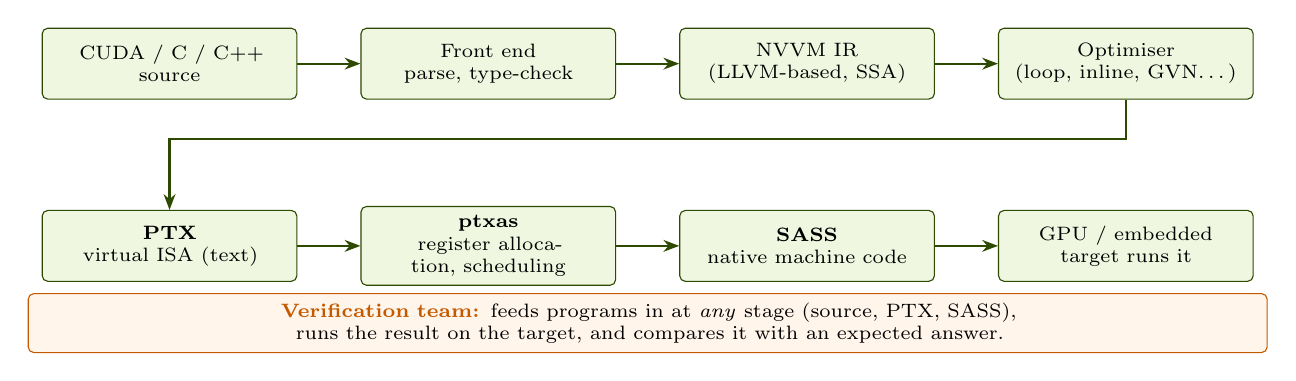
\begin{tikzpicture}[node distance=7mm and 8mm,every node/.style={font=\scriptsize},
 box/.style={draw=nvdark,fill=nvgreen!12,rounded corners=2pt,minimum height=9mm,align=center,text width=3.0cm},
 arr/.style={-{Stealth[length=2mm]},thick,nvdark}]
\node[box] (src) {CUDA / C / C++\\ source};
\node[box,right=of src] (fe) {Front end\\ parse, type-check};
\node[box,right=of fe] (ir) {NVVM IR\\ (LLVM-based, SSA)};
\node[box,right=of ir] (opt) {Optimiser\\ (loop, inline, GVN\ldots)};
\node[box,below=14mm of src] (ptx) {\textbf{PTX}\\ virtual ISA (text)};
\node[box,right=of ptx] (ptxas) {\textbf{ptxas}\\ register allocation, scheduling};
\node[box,right=of ptxas] (sass) {\textbf{SASS}\\ native machine code};
\node[box,right=of sass] (gpu) {GPU / embedded\\ target runs it};
\draw[arr] (src)--(fe); \draw[arr] (fe)--(ir); \draw[arr] (ir)--(opt);
\draw[arr] (opt.south) -- ++(0,-5mm) -| (ptx.north);
\draw[arr] (ptx)--(ptxas); \draw[arr] (ptxas)--(sass); \draw[arr] (sass)--(gpu);
\node[draw=srcorange,fill=orange!8,rounded corners=2pt,align=center,text width=15.5cm,below=6mm of $(ptxas)!0.5!(sass)$]
 {\textcolor{srcorange}{\textbf{Verification team:}} feeds programs in at \emph{any} stage (source, PTX, SASS), runs the result on the target, and compares it with an expected answer.};
\end{tikzpicture}
\end{center}

Two ideas to keep in your head for the whole day:
\begin{enumerate}
\item \textbf{PTX is a virtual ISA; SASS is the real machine code.} The same PTX text can be assembled (by \texttt{ptxas}) for different GPU
 generations, or JIT-compiled by the driver at run time. Writing tests directly in PTX lets the team test the back end without any
 front-end noise.
\item \textbf{``Embedded'' compilers} target NVIDIA's Arm-based SoC platforms and the small processors inside GPUs. NVIDIA publicly states
 that its GPU microcontrollers moved from the proprietary Falcon design to RISC-V
 (\src{https://tomshardware.com/pc-components/gpus/nvidia-to-ship-a-billion-of-risc-v-cores-in-2024}{Tom's Hardware}). Embedded
 verification adds cross-compilation, simulators/boards, code-size limits and sometimes \textbf{functional-safety} rules such as ISO~26262
 (one senior compiler-verification posting asks for it; Chapter~\ref{ch:verif}).
\end{enumerate}

\begin{trapbox}[Do not confuse the two ``verification'' jobs]
NVIDIA also hires \emph{chip design-verification} interns (SystemVerilog/UVM, FIFO-depth maths, FSMs, muxes). Several Glassdoor reports that you
will find when you search ``NVIDIA verification intern interview'' are \textbf{that} job (for example the 2020 and 2025 Santa Clara reports with
FIFO-depth questions). Your role is \emph{software} compiler verification: C/C++, Python, PTX/CUDA, compilers. Ignore RTL/UVM material unless your
invitation says otherwise.
\end{trapbox}

\section{A typical week (inferred from public job postings) \prio{2}}
\begin{enumerate}
\item \textbf{Read the spec.} A new PTX instruction or a C++ feature lands. You read the ISA/standard text and list its corner cases.
\item \textbf{Write tests.} Hand-written directed tests for each corner case, plus \emph{generated} tests: parameterised PTX templates, random program
 generators (Csmith-style), combinatorial sweeps over types, modifiers and rounding modes.
\item \textbf{Run at scale.} A Python runner compiles each test at several optimisation levels/targets, runs it (on a GPU, a simulator or an
 embedded board), enforces timeouts, and stores results.
\item \textbf{Compare.} Results are compared with an \emph{oracle}: another compiler, a CPU reference, the unoptimised build, or a self-checking assertion.
\item \textbf{Triage.} Failures are de-duplicated, minimised (delta-debugging), bisected to the compiler change that introduced them, and filed with a
 small reproducer.
\item \textbf{Close the loop.} The reproducer becomes a permanent regression test; metrics (pass rate, crash rate, coverage) are reported to compiler and
 hardware teams.
\end{enumerate}

\begin{mustbox}[Five habits interviewers want to hear]
\begin{enumerate}[nosep]
\item \textbf{The specification is the law.} Know the difference between undefined, unspecified and implementation-defined behaviour; a ``failing'' test that relies on UB is a bad test, not a compiler bug.
\item \textbf{Tests must be deterministic and self-checking} (fixed seeds, no uninitialised reads, no data races, tolerance for floating-point).
\item \textbf{Minimise before you report} (a 3-line reproducer beats a 3000-line one).
\item \textbf{Automate everything repeatable} (if you did it twice, script it).
\item \textbf{Measure} (coverage, pass rate, time-to-triage); claims without numbers are weak.
\end{enumerate}
\end{mustbox}

\section{The bug zoo \prio{3}}
\begin{center}
\small
\begin{tabularx}{\textwidth}{@{}L{3.1cm}Y@{}}
\toprule
\textbf{Failure class} & \textbf{What it looks like}\\
\midrule
ICE / crash & Compiler aborts or segfaults (``internal compiler error''), even on valid input\\
Hang / timeout & Compiler or compiled program never terminates (often a pass in an infinite loop)\\
\textbf{Miscompilation} & Compiles fine, produces the \emph{wrong result}; usually the most severe class (silent wrong code)\\
Accepts invalid / rejects valid & Front-end bug: a program that violates the spec compiles, or a legal program is refused\\
Wrong diagnostics & Missing or misleading error/warning message\\
Performance regression & Optimised code slower (or larger) than the previous release or than a competitor\\
Debug-info / ABI bug & Debugger shows wrong values; calling convention or struct layout mismatch between modules\\
Non-determinism & Different output on different runs of the same build (data race, uninitialised memory, iteration order)\\
\bottomrule
\end{tabularx}
\end{center}

\begin{tipbox}[Exam tip -- yaad rakho]
If an MCQ says ``which of the following is the most dangerous compiler bug'', the expected answer is almost always \emph{miscompilation (silent wrong code)}.
\end{tipbox}


% ===== 02-intel.tex.in =====
\chapter{Exam Intelligence: What Candidates Actually Reported}
\label{ch:intel}

\begin{chapbox}
\textbf{Read time: 20 min.} This chapter collects what public candidate reports say about NVIDIA's compiler-intern and software-intern
OA/interviews, then turns it into a study-weight table. It is the evidence behind the priorities in the rest of the book.
\end{chapbox}

\begin{trapbox}[How this evidence was gathered -- read this first]
\begin{itemize}
\item The reports were found with web search (GeeksforGeeks, Jointaro, Glassdoor, LeetCode Discuss, placement blogs, job boards). The
research sandbox could \emph{not} open those sites directly (network policy), so the details below come from \textbf{search-engine
summaries of the pages}, not from the pages themselves. Open the numbered links in Section~\ref{tab:sources} to read the originals.
\item Reddit threads could not be retrieved at all (the search tool does not index Reddit); if you have time, search
\emph{``NVIDIA intern OA''} on r/developersIndia and r/Btechtards yourself.
\item All reports are anonymous, small-sample anecdotes spread over 2016--2026, for different teams and cities. \textbf{Nothing here is
official NVIDIA information.} Where two summaries of the same source disagreed, this chapter says so instead of picking one.
\end{itemize}
\end{trapbox}

\section{Reports specific to compiler roles \prio{3}}
{\small\setlength{\tabcolsep}{3pt}
\begin{longtable}{@{}>{\raggedright\arraybackslash}p{2.1cm}>{\raggedright\arraybackslash}p{3.1cm}p{10.6cm}@{}}
\toprule
\rowcolor{orange!22}\textbf{Source} & \textbf{Role / place / year} & \textbf{Reported by candidates: compiler-role interviews and OAs}\\
\midrule
\endfirsthead
\toprule
\rowcolor{orange!22}\textbf{Source} & \textbf{Role / place / year} & \textbf{(continued)}\\
\midrule
\endhead
\textbf{[S1]} GfG & Compiler intern (6 months); page updated Jul 2025 &
 \textbf{R1 online test:} 21 MCQs on C/C++, programming, data structures and \emph{compiler output}, plus one coding question; ``fairly
 straightforward if C/C++ and DS fundamentals are solid''; about 25 candidates reached interviews.
 \textbf{R2 live ``bug hunt'':} a $\sim$250-line C program (binary tree $\to$ doubly linked list in spiral order); 5--10 minutes to find bugs. The
 candidate spotted missing overflow/underflow checks in the stack code but \textbf{missed a call-by-value bug}; follow-up questions on memory allocation.\\
\textbf{[S2]} GfG & LLVM compiler intern, Fall 2025 &
 Four rounds. OA on HackerEarth (core CS fundamentals). Technical rounds: C++ output and recurrences; a chessboard DSA problem (king from
 $(1,1)$ to $(8,8)$: all paths and the shortest); how virtual memory maps to physical memory; analysing a code snippet for variable values and
 memory locations; basic compiler optimisations. Managerial round: motivation, project challenges, \textbf{phases of a compiler, code-generation
 stages, optimisation stages}.\\
\textbf{[S3]} GfG & LLVM compiler intern (6M, spring) &
 OA on C/C++, data structures and compiler design; technical rounds on code output and cycle detection in a linked list.\\
\textbf{[S4]} Jointaro / Glassdoor & Compiler intern, Pittsburgh, Nov 2024 &
 Round 1 (senior manager): topological sort, which turned into \textbf{automatic differentiation and data-flow analysis}; ``why do compilers do
 loop unrolling?''; mostly theoretical. Round 2: \textbf{pointer analysis, dependence analysis}, architectural considerations behind optimisations.\\
\textbf{[S5]} Jointaro / Glassdoor & Compiler intern, Austin, Apr 2025 &
 45-minute virtual round: projects (C++ and GPU), then a short C++ class: \textbf{which constructors and destructors run at each step, and what
 memory-management problems exist}. Verbal reasoning; no live coding.\\
\textbf{[S6]} Jointaro / Glassdoor & Compiler intern, Shanghai, Mar 2024 &
 OA plus technical interview. ``Program \textbf{matrix multiplication} and describe \textbf{all} applicable optimisations (they mean all)''; ``program
 \textbf{graph colouring}''.\\
\textbf{[S7]} Glassdoor & Compiler intern, Bengaluru, Nov 2023 (accepted; applied via university) &
 DSA-centred: a \textbf{2-D knapsack} DP problem, stack operations, and compiler-related questions. Process took about two months.\\
\textbf{[S8]} Glassdoor & Compiler engineer (full-time) &
 ``\textbf{Loop unrolling}''; given a concrete IR example: how would the compiler perform the \emph{most aggressive optimisation}, and what are the trade-offs?\\
\textbf{[S9]} LeetCode Discuss & Compiler engineer, Pune, Sep 2021 (reject) &
 Only a fragment was visible: first round cancelled, coding interviewers gave no hints. (Open the thread for details.)\\
\textbf{[S10]} ProgramHelp & NVIDIA intern virtual onsite (\textbf{low confidence}) &
 Reported topics: constant substitution, loop unrolling, function inlining, code reordering, the \emph{motivation} for unrolling and inlining, and the LLVM IR
 \texttt{getelementptr} instruction with the \texttt{inbounds} flag. A second search could not re-confirm this; treat as plausible topics, not as fact.\\
\bottomrule
\end{longtable}}

\section{Reports on the online assessment format \prio{3}}
{\small\setlength{\tabcolsep}{3pt}
\begin{longtable}{@{}>{\raggedright\arraybackslash}p{2.1cm}>{\raggedright\arraybackslash}p{3.1cm}p{10.6cm}@{}}
\toprule
\rowcolor{orange!22}\textbf{Source} & \textbf{Role / place / year} & \textbf{Reported by candidates: OA format (software roles; mostly India)}\\
\midrule
\endfirsthead
\toprule
\rowcolor{orange!22}\textbf{Source} & \textbf{Role / place / year} & \textbf{(continued)}\\
\midrule
\endhead
\textbf{[S11]} GfG & System software intern, on-campus drive, Mar 2025 &
 HackerRank, about 60 minutes, proctored in college labs: roughly \textbf{28 MCQs + 2 coding problems} on aptitude, data structures, algorithms
 and OS. About 700--800 applicants, about 500 shortlisted for the OA.\\
\textbf{[S12]} GfG & System software intern, on-campus 2024 &
 HackerRank, 50 minutes: aptitude, maths and C MCQs. Another summary of the same site says $\sim$25 MCQs on C/C++, OS, DSA and probability, and that
 the follow-up interview \emph{reused questions from the OA}. One summary mentions \textbf{negative marking}; others say none (varies by drive).\\
\textbf{[S13]} GfG / LeetCode & SDE intern (6 months), on-campus, Feb 2024 &
 OA: 2 CP/DSA problems + aptitude, ``medium to hard''; result in 2--3 days. Interview~1: a \textbf{Trie} problem and a DP problem
 (partition an array to minimise the sum difference), both LeetCode-hard-like.\\
\textbf{[S14]} Glassdoor (Pune) & System software, Pune, 2025 &
 60-minute HackerRank with \textbf{2 coding questions plus C++/Python, Linux and analytical questions}.\\
\textbf{[S15]} Jointaro & Software intern, New Delhi, Oct 2025 &
 Topics listed: \textbf{COA, OS, DSA, puzzles, DBMS}; online coding assessments followed by several technical interviews.\\
\textbf{[S16]} Jointaro / Glassdoor & Hardware interns, India, 2021--2025 &
 Digital-design MCQs then two HackerRank C/C++ problems in one hour (camera-proctored, easy--medium; one was ``find the missing element in an array'').
 Another: \textbf{15 questions in 50 minutes}, including a probability question about three vehicles. Another: 60 minutes of digital electronics, aptitude,
 puzzles and computer architecture.\\
\textbf{[S17]} Jointaro (older) & Bengaluru CAD/ASIC and systems software, 2016--2020 &
 OA with MCQs and two C questions; a HackerRank round on \textbf{bit-shifting of characters}; an interview round on ``C only: memory allocation and bits''.\\
\textbf{[S18]} University / blog pages & General NVIDIA SWE &
 75-minute HackerRank screen with at least two DSA problems plus MCQs; another source: 3 coding questions in 90 minutes; ``format depends on the team'':
 one team reportedly \textbf{C only}, another 7 questions in 50 minutes, another 1 question in 25 minutes. Placement blogs quote 2--3 coding questions,
 15--20 technical MCQs and 10--15 aptitude questions, clear rate 10--15\% (SEO-style pages; weakest evidence).\\
\textbf{[S19]} Glassdoor & Software (Yokneam), Nov 2025 &
 Take-home HackerRank with three coding problems; reported items: palindrome check, \textbf{shuffle a playlist so same-artist songs are not adjacent};
 verbal: a data structure with \textbf{O(1) init / get / set / reset}.\\
\textbf{[S20]} GfG (old) & On-campus, c.\ 2018 &
 40-question written test, no negative marking (C/C++ output, OS, aptitude); technical: pair-sum in C (first $O(n^2)$, then optimised);
 final round: C++ and puzzles.\\
\textbf{[S21]} GfG (tag index) & On-campus, c.\ 2022 &
 Test covered aptitude, C fundamentals, OOP, code snippets, programming, and ``\textbf{AI or statistics}'' -- the only hint of ML-flavoured MCQs.\\
\textbf{[S22]} LeetCode Discuss & SWE, off-campus 2023 &
 A hard \textbf{pointer-output} question; ``\textbf{is the compiler little- or big-endian?}''; where each variable is stored (static / local / global / dynamic);
 templates and inline functions.\\
\textbf{[S23]} GfG & Bengaluru infrastructure team, on-campus &
 Written test: \textbf{C++ concepts, virtual functions, abstract classes, output programs, extern variables, compilation errors}.\\
\textbf{[S24]} Glassdoor (C++ roles) & C++ developer / first rounds &
 Write a C++ class with \textbf{operator overloading and a copy constructor}; deep vs.\ shallow copy; stack vs.\ heap; \textbf{RAII}.\\
\textbf{[S25]} Exponent & SWE &
 \textbf{memcpy / memmove from scratch}; design an \textbf{LRU cache}.\\
\bottomrule
\end{longtable}}

\section{Job-posting evidence \prio{2}}
\begin{itemize}
\item \textbf{Intern posting} (Built~In, ``Compiler Verification Intern -- Fall 2025'', [J1]): build verification infrastructure for NVIDIA embedded platforms; requires strong
 C/C++ \& Python; stand-out: compilers \& ML projects, parallel programming or automation. This is the same text as your role description.
\item \textbf{Pune listing} ([J4], a third-party notice for ``Compiler Verification Intern -- Fall 2026, Pune'') says B.Tech/M.Tech CS, Electrical, Electronics or IT students may apply
 and that duration/stipend are not stated in the posting itself.
\item \textbf{Senior postings} ([J2], [J3]): additionally list \emph{machine learning, formal verification and fuzzing} to automate compiler verification,
 scripting in Python/shell/Perl, compiler front-end or LLVM experience as a plus, and (in one posting only) ISO~26262 functional-safety verification.
\item \textbf{Related compiler postings} ([J6]): ``LLVM and MLIR compiler engineer'' expects loop, inter-procedural and global optimisations and strong C++.
\end{itemize}

\section{What the evidence says \prio{3}}
\begin{center}
\small
\begin{tabularx}{\textwidth}{@{}L{4.4cm}C{1.9cm}Y@{}}
\toprule
\textbf{Topic} & \textbf{Reports mentioning it (of 25)} & \textbf{What to take from it}\\
\midrule
C/C++ output \& memory (ctor/dtor, pointers, endianness, storage, call-by-value, virtual) & $\approx$9 & The most consistent theme. Practise \emph{predicting output} of tricky snippets and \emph{finding bugs} in a page of C.\\
DSA coding (trees, linked lists, DP, graphs, Trie, heap, bit tricks) & $\approx$12 & Expect 1--3 problems of easy--medium level; for the interview, medium--hard in the style of LeetCode.\\
Compiler optimisation \emph{concepts} (loop unrolling, inlining, data-flow, pointer/dependence analysis, graph colouring, matrix-multiply optimisations) & $\approx$6 & Interview favourite. Know \emph{why} each optimisation helps, when it hurts, and how the compiler decides.\\
Compiler basics (phases, code generation, optimisation stages) & $\approx$3 & Easy marks in MCQs and the managerial round.\\
OS / computer architecture (virtual memory, scheduling, caches) & $\approx$5 & Appears in OA MCQs and in compiler interviews (virtual$\to$physical memory).\\
Aptitude, probability, puzzles & $\approx$6 & Light but present; do not skip the probability and permutation basics.\\
ML / statistics & $\approx$1 & Your OA table lists ``ML exposure'', so expect a few conceptual MCQs; breadth over depth.\\
GPU/CUDA/PTX specifics & few & Not reported for \emph{intern} OAs, but the JD names PTX/CUDA; interviewers may ask conceptual questions (warps, divergence, memory spaces).\\
\bottomrule
\end{tabularx}
\end{center}

\begin{mustbox}[Study weights this book uses (derived from the reports above)]
\begin{enumerate}[nosep]
\item \textbf{C/C++ output prediction, memory, UB} (largest, because it is simultaneously OA, interview and the job).
\item \textbf{DSA coding} with fast, bug-free C++/Python templates.
\item \textbf{Compiler theory}: phases, parsing tables, IR/SSA, data-flow, \emph{loop optimisations}, register allocation (graph colouring), linking.
\item \textbf{Aptitude \& probability} (cheap marks; short formulas).
\item \textbf{OS/COA essentials} (virtual memory, scheduling, caches, number representation).
\item \textbf{ML basics} (metrics, bias--variance, neural-net basics, ML compilers).
\item \textbf{LLVM/PTX/CUDA concepts} (differentiators in the interview; know the vocabulary).
\item \textbf{Verification methodology} (differential testing, fuzzing, reduction): the \emph{job itself}; interviewers love candidates who can speak about it.
\end{enumerate}
\end{mustbox}

\section{Your probable OA, reconstructed \prio{3}}
Putting the reports together, the most probable shape (to be confirmed by your invitation) is a single HackerRank session of roughly 60--90 minutes:
\begin{center}
\small
\begin{tabularx}{\textwidth}{@{}L{3.2cm}L{2.7cm}Y@{}}
\toprule
\textbf{Section} & \textbf{Likely size} & \textbf{Content}\\
\midrule
Aptitude & 10--15 MCQs & Percentages, ratios, time--work, probability, permutations, series, logical reasoning, a puzzle or two\\
Technical MCQs & 15--25 MCQs & C/C++ output and concepts; Python snippets; data structures; OS/COA; compiler theory (parsing, optimisation, phases); a few ML questions\\
Coding & 1--3 problems & Array/string/bit manipulation, hashing, sorting, linked list/tree, DP; usually C/C++ or Python (check the language list; one report says a team accepted C only)\\
\bottomrule
\end{tabularx}
\end{center}

\begin{tipbox}[Time budget for a 75-minute paper (adapt to yours)]
Spend about 12 minutes on aptitude, 25 minutes on technical MCQs (30 seconds per MCQ you know; skip anything slower than 2 minutes), and 35 minutes on coding
(easy problem first). Reserve the last 3 minutes to re-check edge cases and remove debug prints. Details in Chapter~\ref{ch:plan}.
\end{tipbox}

\section{Interview style, as reported \prio{2}}
\begin{itemize}
\item \textbf{Format:} one or two technical rounds (30--60 minutes), then a managerial/HR round; some compiler loops are \emph{entirely verbal} (no coding).
\item \textbf{Code reading beats code writing:} ``find the bugs in this C program'', ``which constructors run'', ``what is the output'' (S1, S3, S5).
\item \textbf{Theory with trade-offs:} ``why unroll loops?'', ``what is the downside of aggressive optimisation?'' (S4, S8). Always answer in the pattern
 \emph{benefit $\to$ cost $\to$ when the compiler decides to do it}.
\item \textbf{Projects matter:} Austin and Pune reports start with projects (C++/GPU/compilers). Prepare a 2-minute story per project (Chapter~\ref{ch:flash}).
\item \textbf{The OA is reused:} one report says interview questions repeated OA questions; keep a list of every OA question you remember afterwards.
\end{itemize}

\section{Source list}
\label{tab:sources}
\footnotesize
\setlength{\parskip}{1pt}
\textbf{Candidate reports}\par
\begin{description}[leftmargin=1.2cm,labelwidth=1cm,itemsep=0.5pt,topsep=1pt,font=\bfseries\footnotesize]
\item[S1] \url{https://www.geeksforgeeks.org/interview-experiences/nvidia-interview-experience-for-compiler-intern-6-months/}
\item[S2] \url{https://www.geeksforgeeks.org/interview-experiences/nvidia-llvm-compiler-engineer-internship-fall-2025/}
\item[S3] \url{https://www.geeksforgeeks.org/interview-experiences/nvidia-interview-experience-llvm-compiler-engineer-6m-spring-internship/}
\item[S4] \url{https://www.jointaro.com/interviews/companies/nvidia/experiences/compiler-engineer-intern-pittsburgh-pa-november-1-2024-no-offer-neutral-cb716c3f/}
\item[S5] \url{https://www.jointaro.com/interviews/companies/nvidia/experiences/compiler-engineer-intern-austin-tx-april-1-2025-no-offer-positive-1674ddef/}
\item[S6] \url{https://www.jointaro.com/interviews/companies/nvidia/experiences/compiler-engineer-intern-shanghai-shanghai-march-1-2024-no-offer-neutral-199e988d/}
\item[S7] \url{https://www.glassdoor.co.in/Interview/NVIDIA-Compiler-Engineer-Intern-Interview-Questions-EI_IE7633.0,6_KO7,31.htm}
\item[S8] \url{https://www.glassdoor.com/Interview/NVIDIA-Compiler-Engineer-Interview-Questions-EI_IE7633.0,6_KO7,24.htm}
\item[S9] \url{https://leetcode.com/discuss/interview-experience/1517813/nvidia-compiler-engineer-pune-india-sep-2021-reject/}
\item[S10] \url{https://programhelp.net/en/vo/nvidia-intern-real-interview-experience/}
\item[S11] \url{https://www.geeksforgeeks.org/interview-experiences/nvidia-system-software-engineer-intern-on-campus-drive-experience/}
\item[S12] \url{https://www.geeksforgeeks.org/interview-experiences/nvidia-interview-experience-for-system-software-engineer-internshipon-campus/}
\item[S13] \url{https://www.geeksforgeeks.org/interview-experiences/nvidia-interview-experience-for-sde-internship-on-campus-2024/} and \url{https://leetcode.com/discuss/interview-experience/4730338/}
\item[S14] \url{https://static.glassdoor.com.ar/Interview/NVIDIA-Interview-Questions-E7633_P51.htm} (Glassdoor listing page)
\item[S15] \url{https://www.jointaro.com/interviews/companies/nvidia/experiences/software-engineer-intern-new-delhi-delhi-october-1-2025-no-offer-positive-9bdac977/}
\item[S16] \url{https://www.jointaro.com/interviews/companies/nvidia/experiences/hardware-intern-india-october-1-2024-no-offer-positive-22ba4975/}, \url{https://www.jointaro.com/interviews/companies/nvidia/experiences/hardware-internship-india-january-8-2025-no-offer-positive-bc6c3d7a/}, \url{https://www.jointaro.com/interviews/companies/nvidia/experiences/hardware-internship-india-march-17-2021-no-offer-positive-36f589b3/}
\item[S17] \url{https://www.jointaro.com/interviews/companies/nvidia/work-experiences/software-systems-engineer-bengaluru-february-5-2020-4-1a44b6c8/}, \url{https://www.jointaro.com/interviews/companies/nvidia/work-experiences/cad-engineer-asic-bengaluru-november-29-2016-1-3da7b8ff/}
\item[S18] \url{https://career.online.ou.edu/blog/2025/02/25/get-a-job-at-nvidia-interview-process-and-top-questions/}, \url{https://www.linkjob.ai/interview-questions/nvidia-hackerrank-test/}, \url{https://www.lodely.com/companies/nvidia/online-assessment}, \url{https://placementpapers.app/nvidia/}
\item[S19] \url{https://www.glassdoor.ie/Interview/NVIDIA-Interview-E7633-RVW101986297.htm}, \url{https://www.glassdoor.sg/Interview/NVIDIA-Interview-E7633-RVW104894219.htm}
\item[S20] \url{https://www.geeksforgeeks.org/?p=228100}
\item[S21] \url{https://geeksforgeeks.org/tag/nvidia}
\item[S22] \url{https://leetcode.com/discuss/post/4032849/nvidia-interview-off-campus-2023}
\item[S23] \url{https://www.geeksforgeeks.org/?p=132922}
\item[S24] \url{https://www.glassdoor.sg/Interview/NVIDIA-Interview-E7633-RVW15149051.htm}, \url{https://www.glassdoor.co.in/Interview/NVIDIA-Interview-E7633-RVW23765350.htm}, \url{https://www.glassdoor.co.uk/Interview/NVIDIA-Interview-E7633-RVW9395333.htm}
\item[S25] \url{https://www.tryexponent.com/experiences/nvidia-software-engineer-interview-90647e}
\end{description}
\textbf{Job postings and context}\par
\begin{description}[leftmargin=1.2cm,labelwidth=1cm,itemsep=0.5pt,topsep=1pt,font=\bfseries\footnotesize]
\item[J1] \url{https://builtin.com/job/compiler-verification-intern-fall-2025/6273014}
\item[J2] \url{https://jointaro.com/jobs/nvidia/compiler-verification-software-developer}
\item[J3] \url{https://builtinbengaluru.in/job/senior-compiler-verification-software-developer/3285594}
\item[J4] \url{https://campusreality.in/notification/nvidia-compiler-verification-intern-fall-2026-pune/}
\item[J5] \url{https://www.nvidia.com/en-eu/about-nvidia/careers/university-recruiting-new/}
\item[J6] \url{https://frontlinesmedia.in/nvidia-is-hiring-llvm-and-mlir-compiler-engineer/}
\end{description}
\normalsize


% ===== 03-plan.tex.in =====
\chapter{The 24-Hour Battle Plan and OA Tactics}
\label{ch:plan}

\begin{chapbox}
\textbf{Read time: 15 min.} A time-boxed schedule (with a 6-hour and a 12-hour cut), exam-day tactics, and HackerRank mechanics with templates that
were compiled and run while building this book.
\end{chapbox}

\section{Choose your budget \prio{3}}
\begin{center}
\small
\begin{tabularx}{\textwidth}{@{}L{2.5cm}L{2.2cm}Y@{}}
\toprule
\textbf{Budget} & \textbf{Study hours} & \textbf{What to do}\\
\midrule
\textbf{P1: panic} & 6 h & Only three-star sections. C/C++ output traps (Ch.\,\ref{ch:c}, \ref{ch:cpp}), compiler theory essentials (Ch.\,\ref{ch:front}--\ref{ch:opt}: phases, FIRST/FOLLOW, LR basics, optimisations, data-flow), two timed coding problems (Ch.\,\ref{ch:dsa}), aptitude formula sheet (Ch.\,\ref{ch:apt}), one 45-minute mini-mock.\\
\textbf{P2: normal} & 12 h & P1 \emph{plus}: Python gotchas (Ch.\,\ref{ch:python}), OS/COA essentials (Ch.\,\ref{ch:cs}), ML quick pass (Ch.\,\ref{ch:ml}), LLVM/PTX/CUDA vocabulary (Ch.\,\ref{ch:llvm}--\ref{ch:cuda}), verification vocabulary (Ch.\,\ref{ch:verif}), full mock OA.\\
\textbf{P3: full} & $\sim$14 h & Everything below, including the automation lab (Ch.\,\ref{ch:lab}), interview flashcards (Ch.\,\ref{ch:flash}) and a second set of timed coding problems.\\
\bottomrule
\end{tabularx}
\end{center}

\section{Hour-by-hour plan (P3, adjust to your OA time) \prio{3}}
Hours are counted from the moment you start. About 14 hours of focused work plus meals/breaks plus 7 hours of sleep fits inside 24 hours; if the OA is in the
morning, put the sleep \emph{before} the last two blocks and do those after waking.

{\small
\setlength{\tabcolsep}{3pt}
\begin{longtable}{@{}L{1.9cm}L{3.4cm}L{2.0cm}p{8.1cm}@{}}
\toprule
\textbf{Time (H+)} & \textbf{Block} & \textbf{Chapters} & \textbf{Done when \ldots}\\
\midrule
\endhead
0:00--0:30 & Orientation & 1, 2, 3 & You can state the OA shape, the priorities, and today's schedule. Install/open a local C++ and Python environment.\\
0:30--2:30 & \textbf{C and C++} (output traps, UB, memory, OOP, STL) & 4, 5 & $\ge$80\% on the output-prediction drills; every miss logged with the rule behind it.\\
2:30--2:45 & Break & & Water, walk, no phone.\\
2:45--4:15 & \textbf{Compilers I}: phases, lexing, parsing (FIRST/FOLLOW, LL(1), LR/SLR) & 8, 9 & You can compute FIRST/FOLLOW, an LL(1) table and an LR(0) automaton on paper.\\
4:15--5:45 & \textbf{Compilers II}: semantic analysis, IR/SSA, runtime, \textbf{optimisation}, data-flow, code generation, linking & 10, 11 & You can run reaching-definitions by hand, explain six loop optimisations, and colour a small interference graph.\\
5:45--6:15 & Meal & & \\
6:15--7:30 & \textbf{LLVM, PTX, CUDA}: IR reading, FileCheck, vecadd PTX line by line, warps/divergence/memory spaces & 12--16 & You can read the vecadd PTX aloud and explain every instruction.\\
7:30--8:30 & \textbf{Verification methodology + automation lab} & 17, 18 & You can explain differential testing, EMI, fuzzing, delta debugging; you ran the lab scripts.\\
8:30--9:15 & Python data model and gotchas & 6 & 100\% on the Python drills.\\
9:15--9:45 & Dinner break & & \\
9:45--10:30 & ML quick pass (metrics, bias--variance, neural nets, ML compilers) & 19 & You can compute precision/recall/F1 and explain backprop in four sentences.\\
10:30--11:30 & \textbf{Aptitude} (formulas + 30 timed questions) & 21 & 30 questions in 40 minutes, $\ge$75\% correct.\\
\multicolumn{4}{c}{\textcolor{nvdark}{\textbf{--- Sleep 7 hours (do not skip; recall and focus beat one more chapter) ---}}}\\
+0:00--1:30 & \textbf{Coding practice} (timed) & 7 & Two reported problems solved in $\le$25 min each in C++ \emph{and} one in Python.\\
+1:30--2:15 & OS, computer architecture, number systems & 20 & Virtual memory, scheduling, caches, IEEE-754 reviewed.\\
+2:15--3:30 & \textbf{Mock OA} (full length, strict timing) & 22 & Score logged; every error classified (concept / careless / time).\\
+3:30--4:00 & Interview flashcards, project stories & 23 & Two-minute story for each project; ten rapid-fire answers out loud.\\
+4:00--4:20 & Final 20 minutes: ``Top-40 card'' & App.\,\ref{app:top40} & Re-read, then stop. Check logistics.\\
\bottomrule
\end{longtable}}

\begin{tipbox}[How to study so that it sticks -- active recall]
\begin{enumerate}[nosep]
\item \textbf{Cover the answer, attempt, then read.} For every \texttt{Q}$n.m$ write your answer first (even a guess).
\item \textbf{Keep an error log} (one line per miss: topic, wrong belief, correct rule). Re-read the log, not the chapters, in the last hour.
\item \textbf{Type, do not just read.} Compile every output-prediction snippet you got wrong; the compiler is the examiner you can interrogate.
\item \textbf{50/10 rhythm:} 50 minutes focus, 10 minutes off. Meals and sleep are part of the plan.
\end{enumerate}
\end{tipbox}

\section{Tactics inside the OA \prio{3}}
\begin{enumerate}
\item \textbf{Spend the first 2 minutes reading the whole paper.} Note section sizes, any section-level time limits, whether you can go back, and the
 language list for coding questions.
\item \textbf{Attack order:} fastest marks first. Usually aptitude and short MCQs, then the \emph{easier} coding problem, then harder MCQs, then the other coding problem.
 If sections are individually timed and locked, follow the lock order instead.
\item \textbf{MCQ discipline:} at most 90 seconds per MCQ; mark and move. For code-output MCQs: first look for \emph{traps} (UB, integer promotion, operator precedence,
 off-by-one, uninitialised variable, missing \texttt{break}, macro side effects, \texttt{sizeof} of a pointer) before computing anything.
\item \textbf{Coding: get partial credit early.} HackerRank scores by test case. Submit a correct brute force quickly, then optimise. Read the constraints first
 (Chapter~\ref{ch:dsa}, complexity table).
\item \textbf{Never leave the last 3 minutes unused:} re-run samples, check edge cases ($n=0$, $n=1$, all equal, negatives, maximum size), delete debug output.
\end{enumerate}

\begin{defbox}[Negative marking: when is guessing correct?]
Suppose a correct answer gives $+1$ and a wrong answer gives $-p$, with $k$ equally likely options after elimination. A blind guess among $k$ options has expected score
\[
E = \frac{1}{k}\cdot 1 - \frac{k-1}{k}\,p .
\]
$E>0 \iff p < \tfrac{1}{k-1}$. For 4 options and the common penalty $p=\tfrac14$: blind guess $E=\tfrac14-\tfrac34\cdot\tfrac14=+\tfrac1{16}>0$;
after eliminating one option ($k=3$) $E=\tfrac13-\tfrac23\cdot\tfrac14=+\tfrac16$. \textbf{Rule:} with no penalty always guess; with $p\le\tfrac13$ guessing is never harmful in
expectation; with a harsher penalty guess only after eliminating options. (Reports differ: some NVIDIA drives had negative marking, some did not --
[S12], [S20]. Check your instructions.)
\end{defbox}

\section{HackerRank mechanics \prio{3}}
\begin{itemize}
\item \textbf{Languages:} pick the one in which you are fastest \emph{and} least likely to overflow. C++ for speed/STL; Python for string/array manipulation and big integers.
 Check the exact language versions in the editor drop-down (they change).
\item \textbf{Run vs.\ Submit:} \emph{Run Code} tests your custom input; \emph{Submit} runs all hidden tests. Many OAs allow limited submissions per question; sample-passing is not full marks.
\item \textbf{Errors:} \emph{Wrong Answer} (logic or format), \emph{Runtime Error} (segfault, exception, \texttt{exit code != 0}, array out of range, divide by zero),
 \emph{Time Limit Exceeded} (complexity), \emph{Compilation Error} (wrong language version or a missing header).
\item \textbf{Proctoring:} reports mention camera-proctored tests (S11, S16, S18). Close other tabs/apps, keep ID ready, avoid leaving full-screen, use a charged laptop and stable network.
\end{itemize}

\subsection{Fast I/O templates (compiled and run)}
\needspace{5\baselineskip}
\begin{lstlisting}[language={[11]C++},title={C++ template: fast input, 64-bit sum}]
#include <bits/stdc++.h>
using namespace std;

int main() {
    ios::sync_with_stdio(false);   // do not mix C stdio and iostream afterwards
    cin.tie(nullptr);              // do not flush cout before every cin
    int n;
    cin >> n;
    vector<long long> a(n);
    for (auto &x : a) cin >> x;
    long long sum = accumulate(a.begin(), a.end(), 0LL);   // 0LL, not 0: avoids int accumulation
    cout << sum << "\n";           // "\n" is faster than endl (no flush)
    return 0;
}
\end{lstlisting}
\begin{lstlisting}[style=out]
6
\end{lstlisting}
\needspace{5\baselineskip}
\begin{lstlisting}[language={Python},title={Python template: read everything at once}]
import sys

def main():
    data = sys.stdin.read().split()          # fastest way to read many numbers
    n = int(data[0])
    a = list(map(int, data[1:1 + n]))
    print(sum(a))

main()
\end{lstlisting}
\begin{lstlisting}[style=out]
6
\end{lstlisting}

\subsection{The silent killers}
\needspace{5\baselineskip}
\begin{lstlisting}[language={C},title={Integer overflow: the classic wrong answer}]
#include <stdio.h>
int main(void) {
    int a = 100000;
    int  bad  = a * a;              /* signed overflow: undefined behaviour (typically wraps) */
    long long good = (long long)a * a;   /* widen BEFORE multiplying */
    printf("%d %lld\n", bad, good);
    return 0;
}
\end{lstlisting}
\begin{lstlisting}[style=out]
1410065408 10000000000
\end{lstlisting}
\begin{trapbox}[Pitfall checklist]
\begin{itemize}[nosep]
\item $10^5\times10^5$ overflows 32-bit \texttt{int}; sums of $10^5$ numbers of size $10^9$ need 64 bits. Cast \emph{before} multiplying: \texttt{(long long)a*b}.
\item C++: \texttt{vector<int> v(n)} then reading \texttt{n} numbers is fine, but \texttt{v.size()-1} on an empty vector underflows (\texttt{size\_t} is unsigned).
\item Python: recursion limit is about 1000 by default; use iteration or \texttt{sys.setrecursionlimit}. Avoid \texttt{input()} in loops of $10^5$ lines.
\item Output format: trailing spaces are usually tolerated, but a missing newline or extra text is not. Print only what is asked.
\item Floating point: print with fixed precision (\texttt{cout<<fixed<<setprecision(6)}) when requested; never compare doubles with \texttt{==}.
\end{itemize}
\end{trapbox}

\section{Test-day checklist \prio{2}}
\begin{itemize}[label=$\square$]
\item Invitation email re-read: date/time zone, duration, sections, languages, negative marking, proctoring rules.
\item Laptop charged and plugged in; browser updated; camera/mic permissions tested in the HackerRank system check; stable network (mobile hotspot as a backup).
\item Government ID and college ID on the desk; quiet room; water; paper and pen for rough work (confirm that paper is allowed).
\item A local C++/Python environment ready only for \emph{warm-up} (not during the test unless allowed).
\item Sleep $\ge$7 hours, a light meal, and a 30-minute warm-up of three easy problems before the test starts.
\end{itemize}


% ===== 04a-c-core.tex.in =====
\part{Programming Foundations}

\chapter{C Programming: Output Traps, Memory and UB}
\label{ch:c}

\begin{chapbox}
\textbf{Priority \prio{3}. Time: 75 min (C) + drills.} C questions are the most consistently reported topic (S1, S3, S12, S17, S20, S22): \emph{predict the output}, \emph{find the bug},
\emph{where does this variable live}, \emph{is the machine little-endian}. And they are the job: a compiler verifier must write C that has \textbf{no undefined behaviour} so that a
wrong result can only be the compiler's fault. All outputs in yellow boxes were produced by compiling and running the code (GCC 13, x86-64 Linux, \texttt{-O0} unless stated).
\end{chapbox}

\section{Memory layout and storage classes \prio{3}}
\begin{defbox}[Where things live in a C program]
\begin{center}\small
\begin{tabularx}{\textwidth}{@{}L{3.1cm}L{4.4cm}Y@{}}
\toprule
\textbf{Segment} & \textbf{Holds} & \textbf{Notes}\\
\midrule
\texttt{.text} & machine code & read-only, executable\\
\texttt{.rodata} & string literals, \texttt{const} globals & read-only; writing is undefined behaviour (usually SIGSEGV)\\
\texttt{.data} & initialised globals and \texttt{static}s & copied from the executable image\\
\texttt{.bss} & zero-initialised (or uninitialised) globals/statics & occupies no space in the file; zeroed by the loader\\
\textbf{heap} & \texttt{malloc}/\texttt{calloc}/\texttt{realloc} memory & grows upward; you must \texttt{free} it; fragmentation possible\\
\textbf{stack} & locals, parameters, return addresses & grows downward on x86-64; automatic lifetime; limited (about 8\,MB default on Linux)\\
\bottomrule
\end{tabularx}
\end{center}
\end{defbox}

The linker's symbol table shows the section class of each global. In \texttt{nm} output: \texttt{T} = text, \texttt{D}/\texttt{d} = initialised data (global/static), \texttt{B} = bss, \texttt{R} = read-only data, \texttt{U} = undefined (resolved at link time).
\begin{lstlisting}[language={C}]
#include <stdlib.h>
int g_init = 5;                 /* initialised global      -> .data (D) */
int g_zero;                     /* uninitialised global    -> .bss  (B) */
const int g_const = 9;          /* const global            -> .rodata (R) */
static int g_static = 7;        /* file-local initialised  -> .data (d) */
const char *msg = "hi";         /* pointer in .data (D); the literal "hi" is in .rodata */
int main(void) {
    int local = 1;              /* stack */
    int *h = malloc(4);         /* h itself on the stack; the 4 bytes on the heap */
    free(h);
    return local + g_init;
}
\end{lstlisting}
\begin{lstlisting}[style=shcmd]
$ gcc -c mem.c -o mem.o && nm mem.o
\end{lstlisting}
\begin{lstlisting}[style=out]
                 U free
0000000000000000 R g_const
0000000000000000 D g_init
0000000000000004 d g_static
0000000000000000 B g_zero
0000000000000000 T main
                 U malloc
0000000000000000 D msg
\end{lstlisting}

\begin{center}\small
\begin{tabularx}{\textwidth}{@{}L{2.2cm}L{3.3cm}L{3.3cm}L{3.0cm}Y@{}}
\toprule
\textbf{Class} & \textbf{Scope} & \textbf{Lifetime} & \textbf{Linkage} & \textbf{Default init}\\
\midrule
\texttt{auto} (default for locals) & block & the block execution & none & indeterminate (garbage)\\
\texttt{register} & block & the block & none & indeterminate; cannot take address in C\\
\texttt{static} (local) & block & whole program & none & zero\\
\texttt{static} (global/function) & file & whole program & \textbf{internal} & zero\\
\texttt{extern} / plain global & file or program & whole program & \textbf{external} & zero\\
\bottomrule
\end{tabularx}
\end{center}

\begin{qn}What does this print?\end{qn}
\begin{lstlisting}[language={C}]
#include <stdio.h>
void counter(void) {
    static int n = 0;      /* initialised once, persists across calls */
    int m = 0;             /* re-created at every call */
    n++; m++;
    printf("%d,%d ", n, m);
}
int main(void) {
    for (int i = 0; i < 3; i++) counter();
    printf("\n");
    return 0;
}
\end{lstlisting}
\needspace{5\baselineskip}
\begin{lstlisting}[style=out,title={Answer: captured output}]
1,1 2,1 3,1 
\end{lstlisting}
The \texttt{static} local keeps its value (1, 2, 3) while the automatic \texttt{m} restarts at 1 each time.

\section{Types, sizes, promotions and conversions \prio{3}}
\subsection{Sizes (LP64: Linux/macOS 64-bit) -- know these cold}
\needspace{5\baselineskip}
\begin{lstlisting}[language={C},title={sizeof on x86-64 Linux (LP64)}]
#include <stdio.h>
#include <stdint.h>
int main(void) {
    printf("char=%zu short=%zu int=%zu long=%zu long long=%zu\n",
           sizeof(char), sizeof(short), sizeof(int), sizeof(long), sizeof(long long));
    printf("float=%zu double=%zu long double=%zu pointer=%zu size_t=%zu\n",
           sizeof(float), sizeof(double), sizeof(long double), sizeof(void *), sizeof(size_t));
    printf("int32_t=%zu int64_t=%zu\n", sizeof(int32_t), sizeof(int64_t));
    return 0;
}
\end{lstlisting}
\begin{lstlisting}[style=out]
char=1 short=2 int=4 long=8 long long=8
float=4 double=8 long double=16 pointer=8 size_t=8
int32_t=4 int64_t=8
\end{lstlisting}
\begin{trapbox}[Platform differences]
On 64-bit \textbf{Windows} (LLP64) \texttt{long} is 4 bytes; on 32-bit systems pointers are 4 bytes. If a question does not name the platform, assume the common LP64 sizes above and
say so. \texttt{sizeof} yields \texttt{size\_t} (unsigned): print it with \texttt{\%zu}.
\end{trapbox}

\subsection{Integer promotions and the usual arithmetic conversions}
\begin{mustbox}
\begin{enumerate}[nosep]
\item Any operand narrower than \texttt{int} (\texttt{char}, \texttt{short}, \texttt{bool}) is first promoted to \texttt{int}.
\item If both operands then have the same signedness, the narrower converts to the wider.
\item If the unsigned operand has rank $\ge$ the signed one, the \textbf{signed operand becomes unsigned}. (So $-1 < 1u$ is false: $-1$ becomes $4294967295$.)
\item Integer division truncates toward zero; \texttt{a\%b} has the sign of \texttt{a} (C99 and later).
\end{enumerate}
\end{mustbox}
\needspace{5\baselineskip}
\begin{lstlisting}[language={C},title={Signed/unsigned traps}]
#include <stdio.h>
int main(void) {
    unsigned int u = 1;
    int i = -1;
    printf("i < u            : %d\n", i < u);          /* -1 converted to unsigned: huge */
    printf("sizeof(int) > -1 : %d\n", sizeof(int) > -1);/* -1 converted to size_t */
    unsigned char c = 200;
    printf("c + c            : %d\n", c + c);           /* promoted to int: 400, not 144 */
    printf("(unsigned char)(c + c): %d\n", (unsigned char)(c + c));
    char s = (char)200;                                   /* implementation-defined: usually -56 */
    printf("(char)200        : %d\n", s);
    printf("-7/2=%d  -7%%2=%d  7/-2=%d  7%%-2=%d\n", -7/2, -7%2, 7/-2, 7%-2);
    printf("sizeof('a')=%zu  sizeof(1 ? 1 : 2.0)=%zu\n", sizeof('a'), sizeof(1 ? 1 : 2.0));
    return 0;
}
\end{lstlisting}
\begin{lstlisting}[style=out]
i < u            : 0
sizeof(int) > -1 : 0
c + c            : 400
(unsigned char)(c + c): 144
(char)200        : -56
-7/2=-3  -7%2=-1  7/-2=-3  7%-2=1
sizeof('a')=4  sizeof(1 ? 1 : 2.0)=8
\end{lstlisting}
\begin{tipbox}[C vs.\ C++ difference worth a mark]
A character constant such as \texttt{'a'} has type \textbf{\texttt{int}} in C (so \texttt{sizeof('a')} is 4) but type \texttt{char} in C++ (so 1). The same one-line program prints 4 compiled as C and 1 compiled as C++ (verified while building this book).
\end{tipbox}

\section{Pointers and arrays \prio{3}}
\begin{mustbox}[Rules that decide most pointer MCQs]
\begin{itemize}[nosep]
\item \texttt{a[i]} is defined as \texttt{*(a+i)}; therefore \texttt{i[a]} is legal and equal. Pointer arithmetic is \textbf{scaled by the pointee size}: \texttt{p+1} advances \texttt{sizeof(*p)} bytes.
\item An array name \emph{decays} to a pointer to its first element in most expressions, \textbf{except} as the operand of \texttt{sizeof}, \texttt{\&}, and a string-literal initialiser.
\item A function parameter declared \texttt{int a[10]} is really \texttt{int *a}: \texttt{sizeof a} inside the function is the pointer size.
\item \texttt{p-q} (same array) has type \texttt{ptrdiff\_t} and counts \emph{elements}. Comparing/subtracting pointers into different objects is undefined.
\item Precedence: postfix \texttt{++ -- () []} $>$ prefix \texttt{++ -- * \& sizeof (cast)} $>$ \texttt{* / \%} \ldots Hence \texttt{*p++} is \texttt{*(p++)}, while \texttt{(*p)++} increments the pointee.
\end{itemize}
\end{mustbox}
\needspace{5\baselineskip}
\begin{lstlisting}[language={C},title={Array vs pointer, decay, and *p++ variants}]
#include <stdio.h>
void f(int a[10]) { printf("inside f: sizeof a = %zu\n", sizeof a); }   /* a is int* */
int main(void) {
    int arr[10] = {0};
    printf("sizeof arr = %zu, elements = %zu\n", sizeof arr, sizeof arr / sizeof arr[0]);
    f(arr);
    printf("sizeof(arr+1) = %zu\n", sizeof(arr + 1));           /* decayed to pointer */

    int a[] = {10, 20, 30};
    int *p = a;
    int x = *p++;           /* x = 10, then p -> a[1] */
    printf("*p++ : x=%d, now *p=%d\n", x, *p);
    int y = (*p)++;         /* y = 20, a[1] becomes 21 */
    printf("(*p)++ : y=%d, a[1]=%d\n", y, a[1]);
    int z = *++p;           /* p -> a[2], z = 30 */
    printf("*++p : z=%d\n", z);
    printf("2[a] = %d, &a[2]-&a[0] = %td\n", 2[a], &a[2] - &a[0]);
    return 0;
}
\end{lstlisting}
\begin{lstlisting}[style=out]
sizeof arr = 40, elements = 10
inside f: sizeof a = 8
sizeof(arr+1) = 8
*p++ : x=10, now *p=20
(*p)++ : y=20, a[1]=21
*++p : z=30
2[a] = 30, &a[2]-&a[0] = 2
\end{lstlisting}
\needspace{5\baselineskip}
\begin{lstlisting}[language={C},title={2-D arrays and pointer-to-array}]
#include <stdio.h>
int main(void) {
    int m[2][3] = {{1, 2, 3}, {4, 5, 6}};
    printf("sizeof m=%zu  sizeof m[0]=%zu  sizeof *m=%zu\n", sizeof m, sizeof m[0], sizeof *m);
    printf("*(*(m+1)+2)=%d  **m=%d  *(m[0]+1)=%d\n", *(*(m + 1) + 2), **m, *(m[0] + 1));
    int (*pa)[3] = m;                 /* pointer to an array of 3 ints */
    printf("pa[1][2]=%d  (pa+1) advances %td bytes\n", pa[1][2], (char *)(pa + 1) - (char *)pa);
    int *ap[2] = {m[0], m[1]};        /* array of 2 pointers */
    printf("ap[1][0]=%d  sizeof ap=%zu\n", ap[1][0], sizeof ap);
    return 0;
}
\end{lstlisting}
\begin{lstlisting}[style=out]
sizeof m=24  sizeof m[0]=12  sizeof *m=12
*(*(m+1)+2)=6  **m=1  *(m[0]+1)=2
pa[1][2]=6  (pa+1) advances 12 bytes
ap[1][0]=4  sizeof ap=16
\end{lstlisting}
\begin{trapbox}[Strings: array vs.\ pointer to literal]
\texttt{char s1[] = "abc";} creates a \emph{modifiable copy} (4 bytes including the NUL). \texttt{char *s2 = "abc";} points to a literal in read-only memory: \texttt{s2[0]='X';} is \textbf{undefined} (typically a crash). \texttt{sizeof s1} is 4, \texttt{sizeof s2} is 8.
\end{trapbox}
\needspace{5\baselineskip}
\begin{lstlisting}[language={C},title={Writing to a string literal crashes (SIGSEGV = signal 11)}]
#include <stdio.h>
int main(void) {
    char *s2 = "abc";
    printf("before\n");
    fflush(stdout);
    s2[0] = 'X';          /* undefined behaviour: literal is in .rodata */
    printf("after\n");
    return 0;
}
\end{lstlisting}
\begin{lstlisting}[style=out]
before
[killed by signal 11]
\end{lstlisting}

\subsection{The const reading rule and function pointers}
Read declarations \textbf{right to left}: \texttt{const int *p} = ``p is a pointer to const int'' (cannot change \texttt{*p}); \texttt{int *const p} = ``p is a const pointer to int'' (cannot change \texttt{p}); \texttt{const int *const p}: neither.
\needspace{5\baselineskip}
\begin{lstlisting}[language={C},title={Modifying through a pointer-to-const does not compile}]
int main(void) {
    int v = 1;
    const int *p = &v;
    *p = 2;          /* error: assignment of read-only location */
    return 0;
}
\end{lstlisting}
\begin{lstlisting}[style=out]
prog.c: In function 'main':
prog.c:4:8: error: assignment of read-only location '*p'
    4 |     *p = 2;          /* error: assignment of read-only location */
      |        ^
\end{lstlisting}

\needspace{5\baselineskip}
\begin{lstlisting}[language={C},title={Function pointers and qsort (comparator must not overflow)}]
#include <stdio.h>
#include <stdlib.h>
static int cmp_asc(const void *a, const void *b) {
    int x = *(const int *)a, y = *(const int *)b;
    return (x > y) - (x < y);      /* NOT x - y: that can overflow for large values */
}
int apply(int (*op)(int, int), int a, int b) { return op(a, b); }
static int add(int a, int b) { return a + b; }
static int mul(int a, int b) { return a * b; }
int main(void) {
    int v[] = {5, -2, 9, 0, 3};
    qsort(v, 5, sizeof v[0], cmp_asc);
    for (int i = 0; i < 5; i++) printf("%d ", v[i]);
    printf("\n%d %d\n", apply(add, 3, 4), apply(mul, 3, 4));
    int (*table[2])(int, int) = {add, mul};    /* array of function pointers */
    printf("%d\n", table[1](5, 6));
    return 0;
}
\end{lstlisting}
\begin{lstlisting}[style=out]
-2 0 3 5 9 
7 12
30
\end{lstlisting}

\section{Undefined, unspecified and implementation-defined behaviour \prio{3}}
\label{sec:ub}
This is the single most important idea for a compiler verifier.

\begin{defbox}[The three kinds of ``unportable'' behaviour]
\begin{description}[leftmargin=0pt,labelindent=0pt,itemsep=1pt]
\item[Undefined behaviour (UB):] the standard imposes \emph{no requirements}. The program may crash, print anything, appear to work, or be optimised into something surprising \textbf{because compilers assume UB never happens}.
\item[Unspecified behaviour:] several outcomes are allowed, none required to be documented (e.g.\ evaluation order of function arguments).
\item[Implementation-defined behaviour:] the implementation must document its choice (e.g.\ \texttt{sizeof(int)}, signedness of plain \texttt{char}, right shift of a negative number).
\end{description}
\end{defbox}

\begin{center}\small
\begin{tabularx}{\textwidth}{@{}L{5.6cm}Y@{}}
\toprule
\textbf{Common undefined behaviour in C} & \textbf{Why a compiler may exploit it}\\
\midrule
Signed integer overflow (\texttt{INT\_MAX+1}) & Lets the optimiser assume \texttt{x+1>x} is always true, widen loop counters, etc.\\
Shift by a negative amount or by $\ge$ the width; left-shifting a 1 into the sign bit & Hardware shifts differ; compilers fold freely\\
Division by zero; \texttt{INT\_MIN / -1} & Traps on x86 (SIGFPE); folded arbitrarily otherwise\\
Out-of-bounds array access, null or dangling dereference, use-after-free, double free & Memory is assumed to be well-formed; optimisers reorder/eliminate accesses\\
Reading an uninitialised automatic variable (in most cases) & Value may differ at each use\\
Modifying a variable twice between sequence points (\texttt{i = i++ + ++i}) & Order of side effects is not fixed\\
Strict-aliasing violation (reading a \texttt{float} through an \texttt{int*}) & Loads/stores of different types are assumed not to alias\\
Modifying a string literal or a \texttt{const} object & Placed in read-only memory\\
Data race on non-atomic objects (C11/C++11) & Memory model assumes race freedom\\
\texttt{printf} with a wrong format specifier / wrong argument count & Varargs ABI mismatch\\
\bottomrule
\end{tabularx}
\end{center}

\subsection{Live demonstration: three compilers, three answers}
\needspace{5\baselineskip}
\begin{lstlisting}[language={C},title={ub1.c: signed overflow hidden in x + 1 > x}]
#include <stdio.h>
#include <limits.h>
int f(int x) { return x + 1 > x; }      /* true for all x --- unless x + 1 overflows (UB) */
int main(void) { printf("%d\n", f(INT_MAX)); return 0; }
\end{lstlisting}
\begin{lstlisting}[style=shcmd]
$ for cc in gcc clang; do for o in -O0 -O2; do echo "$cc $o -> $($cc $o -w ub1.c -o ub1 && ./ub1)"; done; done
\end{lstlisting}
\begin{lstlisting}[style=out]
gcc -O0 -> 1
gcc -O2 -> 1
clang -O0 -> 0
clang -O2 -> 1
\end{lstlisting}
\begin{trapbox}[What that table means]
The same \emph{valid-looking} program prints 1 or 0 depending on compiler and optimisation level (GCC folds the comparison even at \texttt{-O0}; Clang \texttt{-O0} actually wraps).
Neither compiler is wrong, because the program has undefined behaviour. \textbf{If a verification test contains UB, a mismatch between two compilers proves nothing.}
This is why random-program generators such as Csmith are designed around UB avoidance (Chapter~\ref{ch:verif}).
\end{trapbox}
\needspace{5\baselineskip}
\begin{lstlisting}[language={C},title={ub2.c: unspecified evaluation order of function arguments}]
#include <stdio.h>
int main(void) {
    int j = 1;
    printf("%d %d\n", j++, j++);   /* modifies j twice without sequencing: UB (and order is unspecified) */
    return 0;
}
\end{lstlisting}
\begin{lstlisting}[style=shcmd]
$ for cc in gcc clang; do $cc -w ub2.c -o ub2 && echo "$cc: $(./ub2)"; done
\end{lstlisting}
\begin{lstlisting}[style=out]
gcc: 2 1
clang: 1 2
\end{lstlisting}
GCC evaluates the arguments right-to-left here and Clang left-to-right. A correct program must not depend on either order.

\begin{tipbox}[Tools that find UB]
\texttt{gcc/clang -fsanitize=undefined} (UBSan: signed overflow, bad shifts, null/misaligned access), \texttt{-fsanitize=address} (ASan: heap/stack buffer overflow, use-after-free, leaks),
\texttt{-fsanitize=thread}, \texttt{-fsanitize=memory} (Clang), \texttt{-Wall -Wextra}, and \texttt{valgrind}. Example, UBSan output for \texttt{INT\_MAX + 1} on a volatile variable:
\end{tipbox}

\begin{lstlisting}[style=shcmd]
$ gcc -fsanitize=undefined ubsan.c -o ubsan && ./ubsan 2>&1 | sed 's/^[^:]*:/prog.c:/'
\end{lstlisting}
\begin{lstlisting}[style=out]
prog.c:3:48: runtime error: signed integer overflow: 2147483647 + 1 cannot be represented in type 'int'
-2147483648
\end{lstlisting}

\subsection{Well-defined ways to do what people try with UB}
\needspace{5\baselineskip}
\begin{lstlisting}[language={C},title={Type punning: union (legal in C) or memcpy (legal in C and C++)}]
#include <stdio.h>
#include <string.h>
#include <stdint.h>
int main(void) {
    float f = 1.0f;
    union { float f; uint32_t u; } pun = { .f = f };
    uint32_t viaMemcpy;
    memcpy(&viaMemcpy, &f, sizeof f);
    printf("1.0f bits: union=0x%08x memcpy=0x%08x\n", pun.u, viaMemcpy);
    /* uint32_t bad = *(uint32_t *)&f;   <- strict-aliasing violation: undefined */
    unsigned x = 1u << 31;                     /* fine: unsigned */
    printf("1u<<31 = %u\n", x);
    printf("1.0/0 = %f, -1.0/0 = %f\n", 1.0 / 0, -1.0 / 0);   /* IEEE: inf, not UB on IEEE targets */
    return 0;
}
\end{lstlisting}
\begin{lstlisting}[style=out]
1.0f bits: union=0x3f800000 memcpy=0x3f800000
1u<<31 = 2147483648
1.0/0 = inf, -1.0/0 = -inf
\end{lstlisting}

\section{The preprocessor \prio{3}}
\needspace{5\baselineskip}
\begin{lstlisting}[language={C},title={Macro traps: precedence and double evaluation}]
#include <stdio.h>
#define SQ_BAD(x)   x * x
#define SQ_OK(x)    ((x) * (x))
#define MAX(a, b)   ((a) > (b) ? (a) : (b))
#define STR(x)      #x                 /* stringize */
#define CAT(a, b)   a##b               /* token pasting */
int main(void) {
    printf("SQ_BAD(2+3)   = %d   (expands to 2+3 * 2+3)\n", SQ_BAD(2 + 3));
    printf("SQ_OK(2+3)    = %d\n", SQ_OK(2 + 3));
    printf("100/SQ_BAD(5) = %d   (expands to 100/5 * 5)\n", 100 / SQ_BAD(5));
    int a = 3, b = 7;
    int m = MAX(a++, b++);               /* b++ is evaluated twice when b is chosen */
    printf("MAX(a++,b++)  = %d, a=%d, b=%d\n", m, a, b);
    printf("%s, %d\n", STR(hello world), CAT(1, 2) + 1);
    printf("line %d in %s\n", __LINE__, "prog.c");
    return 0;
}
\end{lstlisting}
\begin{lstlisting}[style=out]
SQ_BAD(2+3)   = 11   (expands to 2+3 * 2+3)
SQ_OK(2+3)    = 25
100/SQ_BAD(5) = 100   (expands to 100/5 * 5)
MAX(a++,b++)  = 8, a=4, b=9
hello world, 13
line 15 in prog.c
\end{lstlisting}
\begin{mustbox}[Preprocessor facts]
\begin{itemize}[nosep]
\item Macros are \textbf{textual substitution before parsing}: no types, no scope, no evaluation. Parenthesise every parameter and the whole body.
\item \texttt{\#x} stringizes the argument; \texttt{a\#\#b} pastes tokens; \texttt{\_\_VA\_ARGS\_\_} for variadic macros; \texttt{\_\_LINE\_\_}, \texttt{\_\_FILE\_\_}, \texttt{\_\_func\_\_} (the last is a C99 identifier, not a macro).
\item Multi-statement macros: \texttt{do \{ ... \} while (0)} so they behave as one statement (works with \texttt{if/else}).
\item Include guards (\texttt{\#ifndef X / \#define X / \#endif}) or \texttt{\#pragma once} prevent double inclusion; the preprocessor's output is what the compiler sees (\texttt{gcc -E}).
\item Prefer \texttt{static inline} functions (C) or \texttt{constexpr} functions (C++): typed, debuggable, no double evaluation.
\end{itemize}
\end{mustbox}

\section{Bit manipulation \prio{3}}
Bit tricks appear in OAs (S17: ``bit-shifting operations on characters''), in coding questions, and in every compiler (strength reduction, instruction selection).
\begin{center}\small
\begin{tabularx}{\textwidth}{@{}L{5.6cm}Y@{}}
\toprule
\textbf{Goal} & \textbf{Expression (unsigned \texttt{x}, bit index \texttt{k})}\\
\midrule
Set / clear / toggle / test bit $k$ & \texttt{x | (1u<<k)} \quad \texttt{x \& \textasciitilde{}(1u<<k)} \quad \texttt{x \textasciicircum{} (1u<<k)} \quad \texttt{(x>>k) \& 1u}\\
Lowest set bit (isolate) & \texttt{x \& -x}\quad (two's complement: $-x=\sim x+1$)\\
Clear lowest set bit & \texttt{x \& (x-1)}\quad (Kernighan's popcount loops on this)\\
Is a power of two? & \texttt{x \&\& !(x \& (x-1))}\\
Low $k$ bits mask / extract bits $[i..j]$ & \texttt{(1u<<k)-1} \quad \texttt{(x>>i) \& ((1u<<(j-i+1))-1)}\\
Swap without a temporary & \texttt{a\textasciicircum{}=b; b\textasciicircum{}=a; a\textasciicircum{}=b;} (only for distinct objects; do not write it as one expression)\\
Unique element when all others appear twice & XOR all elements ($a\oplus a=0$, $a\oplus0=a$)\\
Count trailing / leading zeros, popcount (GCC/Clang) & \texttt{\_\_builtin\_ctz(x)}, \texttt{\_\_builtin\_clz(x)}, \texttt{\_\_builtin\_popcount(x)}\\
Round up to the next power of two (32-bit) & \texttt{x--; x|=x>>1; x|=x>>2; x|=x>>4; x|=x>>8; x|=x>>16; x++;}\\
\bottomrule
\end{tabularx}
\end{center}
\needspace{5\baselineskip}
\begin{lstlisting}[language={C},title={Bit tricks on x = 0b10110100 (180)}]
#include <stdio.h>
#include <stdint.h>
static int popcount_kernighan(unsigned x) { int c = 0; while (x) { x &= x - 1; c++; } return c; }
int main(void) {
    unsigned x = 0xB4;   /* 1011 0100 */
    printf("x=%u  lowest set bit: x&-x = %u  clear it: x&(x-1) = %u\n", x, x & -x, x & (x - 1));
    printf("popcount=%d (Kernighan %d)  ctz=%d  clz(32-bit)=%d\n",
           __builtin_popcount(x), popcount_kernighan(x), __builtin_ctz(x), __builtin_clz(x));
    printf("is_pow2(64)=%d is_pow2(65)=%d\n", (64 && !(64 & 63)), (65 && !(65 & 64)));
    int a = 6, b = 9;
    a ^= b; b ^= a; a ^= b;
    printf("after xor-swap: a=%d b=%d\n", a, b);
    int arr[] = {4, 7, 4, 9, 7};          /* 9 is the unique one */
    int u = 0; for (int i = 0; i < 5; i++) u ^= arr[i];
    printf("unique = %d\n", u);
    printf("-x == ~x+1 ? %d\n", -(int)x == ~(int)x + 1);
    printf("-16 >> 2 = %d (arithmetic shift on this ABI; implementation-defined)\n", -16 >> 2);
    printf("~5=%d  5<<2=%d  5&3=%d 5|3=%d 5^3=%d\n", ~5, 5 << 2, 5 & 3, 5 | 3, 5 ^ 3);
    return 0;
}
\end{lstlisting}
\begin{lstlisting}[style=out]
x=180  lowest set bit: x&-x = 4  clear it: x&(x-1) = 176
popcount=4 (Kernighan 4)  ctz=2  clz(32-bit)=24
is_pow2(64)=1 is_pow2(65)=0
after xor-swap: a=9 b=6
unique = 9
-x == ~x+1 ? 1
-16 >> 2 = -4 (arithmetic shift on this ABI; implementation-defined)
~5=-6  5<<2=20  5&3=1 5|3=7 5^3=6
\end{lstlisting}
\subsubsection*{Shifting characters (the S17-style trap)}
\needspace{5\baselineskip}
\begin{lstlisting}[language={C},title={Char shifts: promotion to int, truncation on store, and 8-bit rotate}]
#include <stdio.h>
int main(void) {
    unsigned char c = 0x81;                 /* 1000 0001 */
    printf("c << 1            = 0x%x  (promoted to int, NOT truncated)\n", c << 1);
    unsigned char d = c << 1;               /* truncated when stored back */
    printf("(unsigned char)   = 0x%x\n", d);
    signed char s = (signed char)0x81;      /* -127 */
    printf("s >> 1            = %d (sign-extended; implementation-defined)\n", s >> 1);
    unsigned char r = (unsigned char)((c << 1) | (c >> 7));   /* rotate left by 1 */
    printf("rotl8(0x81, 1)    = 0x%x\n", r);
    return 0;
}
\end{lstlisting}
\begin{lstlisting}[style=out]
c << 1            = 0x102  (promoted to int, NOT truncated)
(unsigned char)   = 0x2
s >> 1            = -64 (sign-extended; implementation-defined)
rotl8(0x81, 1)    = 0x3
\end{lstlisting}
\subsubsection*{Endianness check (reported in S22)}
\needspace{5\baselineskip}
\begin{lstlisting}[language={C},title={Is this machine little-endian?}]
#include <stdio.h>
#include <stdint.h>
int main(void) {
    uint32_t v = 0x01020304;
    unsigned char *p = (unsigned char *)&v;     /* char access is always allowed */
    printf("first byte in memory: 0x%02x -> %s-endian\n", p[0], p[0] == 0x04 ? "little" : "big");
    return 0;
}
\end{lstlisting}
\begin{lstlisting}[style=out]
first byte in memory: 0x04 -> little-endian
\end{lstlisting}


% ===== 04b-c-more.tex.in =====
\section{Structs, unions, padding, bit-fields \prio{2}}
\begin{mustbox}[Layout rules]
Each member is placed at an offset that is a multiple of its \emph{alignment} (for scalars: its size). The struct's alignment is the largest member alignment, and its total size is rounded up to a multiple of that.
\textbf{Declare members from largest to smallest to minimise padding.} A \texttt{union}'s size is its largest member's size (rounded up to its alignment); all members share the same bytes. Bit-field ordering and packing are implementation-defined.
\end{mustbox}
\needspace{5\baselineskip}
\begin{lstlisting}[language={C},title={Padding, offsetof, unions, bit-fields}]
#include <stdio.h>
#include <stddef.h>
struct A { char c; int i; char d; };                      /* 1 + 3 pad + 4 + 1 + 3 pad */
struct B { int i; char c; char d; };                      /* 4 + 1 + 1 + 2 pad */
struct __attribute__((packed)) P { char c; int i; char d; };   /* GCC/Clang extension */
struct C { char c; double d; char e; };                   /* double needs 8-byte alignment */
union  U { int i; char c[8]; double d; };
struct BF { unsigned a : 3; unsigned b : 5; unsigned c : 8; };
int main(void) {
    printf("A=%zu (offsets %zu %zu %zu)\n", sizeof(struct A), offsetof(struct A, c), offsetof(struct A, i), offsetof(struct A, d));
    printf("B=%zu (offsets %zu %zu %zu)\n", sizeof(struct B), offsetof(struct B, i), offsetof(struct B, c), offsetof(struct B, d));
    printf("P=%zu  C=%zu  U=%zu  BF=%zu\n", sizeof(struct P), sizeof(struct C), sizeof(union U), sizeof(struct BF));
    return 0;
}
\end{lstlisting}
\begin{lstlisting}[style=out]
A=12 (offsets 0 4 8)
B=8 (offsets 0 4 5)
P=6  C=24  U=8  BF=4
\end{lstlisting}
\begin{tipbox}[Why this matters to a compiler team]
Struct layout is part of the \textbf{ABI}: if two compilers disagree on padding or bit-field placement, code compiled by one cannot call code compiled by the other. ABI/layout tests are a classic verification area.
\end{tipbox}

\section{Dynamic memory \prio{3}}
\begin{mustbox}
\begin{itemize}[nosep]
\item \texttt{malloc(n)}: uninitialised bytes; \texttt{calloc(k,n)}: zeroed, checks \texttt{k*n} overflow; \texttt{realloc(p,n)}: may move the block; on failure returns NULL \emph{and the old block is still valid}, so never write \texttt{p = realloc(p, n)} (leak on failure); \texttt{free(NULL)} is a no-op; \texttt{free} twice is undefined.
\item Idiom: \texttt{T *p = malloc(count * sizeof *p);}\ (type-safe: survives a change of \texttt{T}). Always test for NULL.
\item \textbf{Memory leak} = allocated block unreachable and never freed. \textbf{Dangling pointer} = pointer to freed/expired storage. \textbf{Buffer overflow} = access past the allocation (the root of most security bugs).
\item Allocators (glibc \texttt{malloc}) manage free lists in the heap (\texttt{brk}) and use \texttt{mmap} for large blocks; fragmentation and alignment (16 bytes on x86-64) matter.
\end{itemize}
\end{mustbox}
\needspace{5\baselineskip}
\begin{lstlisting}[language={C},title={2-D array on the heap, safe realloc, then correct cleanup}]
#include <stdio.h>
#include <stdlib.h>
int main(void) {
    int rows = 3, cols = 4;
    int **m = malloc(rows * sizeof *m);
    if (!m) return 1;
    for (int i = 0; i < rows; i++) {
        m[i] = calloc(cols, sizeof **m);          /* zero-initialised row */
        if (!m[i]) return 1;
        for (int j = 0; j < cols; j++) m[i][j] = i * j;
    }
    for (int i = 0; i < rows; i++) { for (int j = 0; j < cols; j++) printf("%d ", m[i][j]); printf("\n"); }
    for (int i = 0; i < rows; i++) free(m[i]);   /* free rows first ... */
    free(m);                                      /* ... then the pointer array */

    int *v = malloc(2 * sizeof *v), cap = 2, n = 0;
    for (int x = 1; x <= 5; x++) {
        if (n == cap) {                           /* amortised O(1) append: double the capacity */
            int *tmp = realloc(v, 2 * cap * sizeof *v);
            if (!tmp) { free(v); return 1; }      /* old block still valid if realloc failed */
            v = tmp; cap *= 2;
        }
        v[n++] = x * x;
    }
    printf("n=%d cap=%d last=%d\n", n, cap, v[n - 1]);
    free(v);
    return 0;
}
\end{lstlisting}
\begin{lstlisting}[style=out]
0 0 0 0 
0 1 2 3 
0 2 4 6 
n=5 cap=8 last=25
\end{lstlisting}
Sanitizers turn silent memory bugs into precise reports. The three classic bugs, each compiled with \texttt{-fsanitize=address} (addresses and process ids removed from the output):



\begin{lstlisting}[style=shcmd]
$ gcc -g -fsanitize=address X.c -o X && ./X     # for X in oob, uaf, leak
\end{lstlisting}
\begin{lstlisting}[style=out]
[oob]
ERROR: AddressSanitizer: heap-buffer-overflow
SUMMARY: AddressSanitizer: heap-buffer-overflow oob.c:2 in main
[uaf]
ERROR: AddressSanitizer: heap-use-after-free
SUMMARY: AddressSanitizer: heap-use-after-free uaf.c:2 in main
[leak]
ERROR: LeakSanitizer: detected memory leaks
SUMMARY: AddressSanitizer: 16 byte(s) leaked in 1 allocation(s).
\end{lstlisting}

\section{Functions, call-by-value and the calling convention \prio{3}}
C passes \textbf{everything by value}: the callee gets a copy of each argument. ``Pass by reference'' means passing a pointer \emph{by value}. This is exactly the bug the S1 candidate missed in a 250-line program.
\needspace{5\baselineskip}
\begin{lstlisting}[language={C},title={Call-by-value: why the head of a linked list is not updated}]
#include <stdio.h>
#include <stdlib.h>
typedef struct Node { int val; struct Node *next; } Node;

void push_bad(Node *head, int v) {          /* head is a COPY of the caller's pointer */
    Node *n = malloc(sizeof *n);
    n->val = v; n->next = head;
    head = n;                               /* updates only the local copy; n leaks */
}
void push_good(Node **head, int v) {        /* pointer to the caller's pointer */
    Node *n = malloc(sizeof *n);
    n->val = v; n->next = *head;
    *head = n;
}
void print_list(const Node *h) { for (; h; h = h->next) printf("%d ", h->val); printf("<end>\n"); }
void swap_val(int a, int b) { int t = a; a = b; b = t; }          /* no effect on the caller */
void swap_ptr(int *a, int *b) { int t = *a; *a = *b; *b = t; }
int main(void) {
    Node *head = NULL;
    push_bad(head, 1); push_bad(head, 2);
    print_list(head);                       /* list is still empty */
    push_good(&head, 1); push_good(&head, 2);
    print_list(head);
    int x = 1, y = 2;
    swap_val(x, y); printf("after swap_val: %d %d\n", x, y);
    swap_ptr(&x, &y); printf("after swap_ptr: %d %d\n", x, y);
    return 0;
}
\end{lstlisting}
\begin{lstlisting}[style=out]
<end>
2 1 <end>
after swap_val: 1 2
after swap_ptr: 2 1
\end{lstlisting}
\subsection{Recursion, stack frames and the System~V AMD64 calling convention}
\begin{mustbox}[x86-64 System V ABI (Linux/macOS) in six lines]
\begin{itemize}[nosep]
\item Integer/pointer arguments: \texttt{rdi, rsi, rdx, rcx, r8, r9}, then the stack (right to left). Floating-point: \texttt{xmm0--xmm7}. Return value: \texttt{rax} (or \texttt{rdx:rax}, \texttt{xmm0}).
\item \textbf{Callee-saved:} \texttt{rbx, rbp, r12--r15} (a function that uses them must restore them). \textbf{Caller-saved:} everything else (\texttt{rax, rcx, rdx, rsi, rdi, r8--r11}, \texttt{xmm}).
\item The stack pointer must be 16-byte aligned at a \texttt{call}; the 128 bytes below \texttt{rsp} (the ``red zone'') may be used by leaf functions without adjusting \texttt{rsp}.
\item A \textbf{stack frame} holds the return address, saved registers, locals and spilled temporaries; deep recursion exhausts the (about 8\,MB) stack: stack overflow.
\end{itemize}
\end{mustbox}
\begin{lstlisting}[language={C}]
int add3(int a, int b, int c) { return a + b + c; }
\end{lstlisting}
\begin{lstlisting}[style=shcmd]
$ gcc -O1 -S -masm=intel add3.c
\end{lstlisting}
\begin{lstlisting}[style=out]
add3:
    add    edi, esi
    lea    eax, [rdi+rdx]
    ret
\end{lstlisting}
The three arguments arrive in \texttt{edi, esi, edx} (the 32-bit halves of \texttt{rdi, rsi, rdx}) and the result leaves in \texttt{eax}: the compiler turned \texttt{a+b+c} into one \texttt{add} and one \texttt{lea} (a 3-operand add in disguise).

\subsection{Variadic functions}
\needspace{5\baselineskip}
\begin{lstlisting}[language={C},title={stdarg: default argument promotions}]
#include <stdio.h>
#include <stdarg.h>
int sum(int n, ...) {
    va_list ap; va_start(ap, n);
    int s = 0;
    for (int i = 0; i < n; i++) s += va_arg(ap, int);   /* char/short arrive as int */
    va_end(ap);
    return s;
}
double avg(int n, ...) {
    va_list ap; va_start(ap, n);
    double s = 0;
    for (int i = 0; i < n; i++) s += va_arg(ap, double); /* float arrives as double: never va_arg(ap, float) */
    va_end(ap);
    return s / n;
}
int main(void) {
    printf("%d %.2f\n", sum(4, 1, 2, 3, 4), avg(3, 1.0, 2.0f, 6.0));
    return 0;
}
\end{lstlisting}
\begin{lstlisting}[style=out]
10 3.00
\end{lstlisting}

\section{Qualifiers: \texttt{volatile}, \texttt{restrict}, \texttt{inline}, \texttt{static} \prio{2}}
\begin{itemize}
\item \textbf{\texttt{volatile}}: every access in the source must be performed (no caching in a register, no elimination). Use for memory-mapped I/O and variables changed by signal handlers. It is \emph{not} atomic and gives no inter-thread ordering.
\item \textbf{\texttt{restrict}} (C99): a promise that, during the pointer's lifetime, the object it points to is accessed only through it (or pointers derived from it). It lets the compiler vectorise; if the promise is false the behaviour is undefined.
\item \textbf{\texttt{inline}}: a hint plus linkage rules. In C99/C11 a plain \texttt{inline} function needs one external definition; \texttt{static inline} avoids that problem.
\item \textbf{\texttt{static}} on a function or global gives it internal linkage (invisible to other translation units).
\end{itemize}
The effect of \texttt{volatile} is visible in the generated code:
\begin{lstlisting}[language={C}]
int flag;                 /* plain */
volatile int vflag;       /* volatile */
void wait_plain(void)    { while (!flag)  { } }
void wait_volatile(void) { while (!vflag) { } }
\end{lstlisting}
\begin{lstlisting}[style=shcmd]
$ gcc -O2 -S -masm=intel vol.c
\end{lstlisting}
\begin{lstlisting}[style=out]
wait_plain:
    mov    eax, DWORD PTR flag[rip]
    test    eax, eax
    jne    .L1
.L3:
    jmp    .L3
.L1:
    ret
wait_volatile:
.L6:
    mov    eax, DWORD PTR vflag[rip]
    test    eax, eax
    je    .L6
    ret
\end{lstlisting}
\begin{trapbox}[Read that assembly]
\texttt{wait\_plain} loads \texttt{flag} \textbf{once}, and if it was 0 jumps to \texttt{.L3: jmp .L3}, an infinite loop: the compiler proved nothing in the loop changes \texttt{flag}. \texttt{wait\_volatile} re-loads \texttt{vflag} on every iteration. This is a legal optimisation, not a compiler bug; correct code needs \texttt{volatile} (or, for threads, \texttt{atomic}).
\end{trapbox}

\section{Standard-library essentials and pitfalls \prio{2}}
\needspace{5\baselineskip}
\begin{lstlisting}[language={C},title={printf format cheat sheet (every specifier here is a classic MCQ)}]
#include <stdio.h>
int main(void) {
    printf("[%5d] [%-5d] [%05d] [%+d] [%*d]\n", 42, 42, 42, 42, 6, 42);
    printf("[%x] [%X] [%#x] [%o] [%#o]\n", 255, 255, 255, 8, 8);
    printf("[%e] [%g] [%g] [%.3f] [%10.2f] [%-10.2f]\n", 1234.5678, 1234.5678, 0.00001234, 3.14159, 3.14159, 3.14159);
    printf("[%c] [%s] [%.3s] [%10s] [%-10s] [%%]\n", 'x', "hello", "hello", "hi", "hi");
    printf("[%zu] [%lld] [%u] [%hhd] [%ld]\n", sizeof(int), 1LL << 40, 4000000000u, (signed char)200, -5L);
    int n = printf("abc\n");                       /* printf returns the number of characters written */
    printf("returned %d\n", n);
    return 0;
}
\end{lstlisting}
\begin{lstlisting}[style=out]
[   42] [42   ] [00042] [+42] [    42]
[ff] [FF] [0xff] [10] [010]
[1.234568e+03] [1234.57] [1.234e-05] [3.142] [      3.14] [3.14      ]
[x] [hello] [hel] [        hi] [hi        ] [%]
[4] [1099511627776] [4000000000] [-56] [-5]
abc
returned 4
\end{lstlisting}
\needspace{5\baselineskip}
\begin{lstlisting}[language={C},title={scanf family and string-function pitfalls}]
#include <stdio.h>
#include <string.h>
int main(void) {
    int a = 0, b = 0;
    int n = sscanf("12 abc", "%d %d", &a, &b);          /* returns the number of items converted */
    printf("sscanf returned %d, a=%d\n", n, a);
    char w[8];
    sscanf("hello world", "%7s", w);                    /* always give %s a width: no bound = overflow */
    printf("[%s]\n", w);

    char buf[4];
    strncpy(buf, "abcdef", sizeof buf);                 /* source too long: NOT null-terminated! */
    buf[sizeof buf - 1] = '\0';                         /* so terminate it yourself */
    printf("%s\n", buf);

    printf("%d %d %d\n", strcmp("a", "b") < 0, strcmp("b", "a") > 0, strcmp("a", "a"));
    char s[] = "a,b,,c"; char *t = strtok(s, ",");      /* strtok modifies its input, merges delimiters, is not re-entrant */
    while (t) { printf("%s|", t); t = strtok(NULL, ","); }
    printf("\n");

    char m[] = "abcdef";
    memmove(m + 2, m, 4);                               /* overlapping copy: only memmove is safe */
    printf("%s\n", m);
    return 0;
}
\end{lstlisting}
\begin{lstlisting}[style=out]
sscanf returned 1, a=12
[hello]
abc
1 1 0
a|b|c|
ababcd
\end{lstlisting}
\begin{trapbox}[Library traps examiners like]
\texttt{gets} was removed in C11 (use \texttt{fgets}, which keeps the newline). \texttt{strcpy/strcat/sprintf} do not check bounds. \texttt{strlen} is $O(n)$, so a loop \texttt{for(i=0;i<strlen(s);i++)} is quadratic. \texttt{memset} sets \emph{bytes} (\texttt{memset(a,1,n)} on ints writes 0x01010101). \texttt{rand()\%n} is biased and not secure. \texttt{atoi} cannot report errors (use \texttt{strtol}). \texttt{printf("\%s", NULL)} is undefined.
\end{trapbox}

\section{Reimplement the library: strlen, strcmp, memcpy, memmove, atoi \prio{3}}
Reported in S25 (``memcpy / memmove from scratch'') and a staple of C interviews. The key insight for \texttt{memmove}: if the destination starts \emph{after} the source and the ranges overlap, copy \textbf{backwards}.
\needspace{5\baselineskip}
\begin{lstlisting}[language={C},title={Library functions from scratch, with tests}]
#include <stdio.h>
#include <string.h>
#include <ctype.h>
#include <limits.h>
#include <assert.h>

size_t my_strlen(const char *s) { const char *p = s; while (*p) p++; return (size_t)(p - s); }
char *my_strcpy(char *d, const char *s) { char *r = d; while ((*d++ = *s++)) ; return r; }
int my_strcmp(const char *a, const char *b) {
    while (*a && *a == *b) { a++; b++; }
    return (unsigned char)*a - (unsigned char)*b;            /* compare as unsigned char, like the standard */
}
void *my_memcpy(void *d, const void *s, size_t n) {          /* regions must NOT overlap */
    unsigned char *dp = d; const unsigned char *sp = s;
    while (n--) *dp++ = *sp++;
    return d;
}
void *my_memmove(void *d, const void *s, size_t n) {
    unsigned char *dp = d; const unsigned char *sp = s;
    if (dp == sp || n == 0) return d;
    if (dp < sp) { while (n--) *dp++ = *sp++; }              /* forward copy is safe */
    else { dp += n; sp += n; while (n--) *--dp = *--sp; }    /* dest after src: copy backwards */
    return d;
}
int my_atoi(const char *s) {
    while (isspace((unsigned char)*s)) s++;
    int sign = 1;
    if (*s == '+' || *s == '-') { if (*s == '-') sign = -1; s++; }
    long long v = 0;
    while (isdigit((unsigned char)*s)) {
        v = v * 10 + (*s - '0');
        if (sign * v > INT_MAX) return INT_MAX;               /* clamp instead of overflowing */
        if (sign * v < INT_MIN) return INT_MIN;
        s++;
    }
    return (int)(sign * v);
}
int main(void) {
    char a[16];
    assert(my_strlen("hello") == 5 && my_strlen("") == 0);
    assert(strcmp(my_strcpy(a, "copy"), "copy") == 0);
    assert(my_strcmp("abc", "abd") < 0 && my_strcmp("b", "a") > 0 && my_strcmp("x", "x") == 0);
    char f[] = "abcdef"; my_memmove(f + 2, f, 4);  printf("memmove forward overlap : %s\n", f);  /* ababcd */
    char g[] = "abcdef"; my_memmove(g, g + 2, 4);  printf("memmove backward overlap: %s\n", g);  /* cdefef */
    printf("atoi: %d %d %d %d\n", my_atoi("  -42abc"), my_atoi("+7"), my_atoi("99999999999"), my_atoi("-99999999999"));
    char h[8]; my_memcpy(h, "xyz", 4); printf("memcpy: %s\n", h);
    puts("all asserts passed");
    return 0;
}
\end{lstlisting}
\begin{lstlisting}[style=out]
memmove forward overlap : ababcd
memmove backward overlap: cdefef
atoi: -42 7 2147483647 -2147483648
memcpy: xyz
all asserts passed
\end{lstlisting}

\section{Find the bugs: the ``bug-hunt'' round \prio{3}}
The S1 interview gave a candidate a 250-line C program and 5--10 minutes to find bugs. The program below is deliberately wrong in at least ten ways. \textbf{Try to list them before reading the answers.}
\begin{lstlisting}[language={C},numbers=left,numberstyle=\tiny\color{gray},stepnumber=1,numbersep=5pt,xleftmargin=16pt]
#include <stdio.h>
#include <stdlib.h>
#include <string.h>

#define CAP 4
typedef struct { int data[CAP]; int top; } Stack;

void push(Stack *s, int v) { s->data[s->top++] = v; }
int  pop(Stack *s)         { return s->data[--s->top]; }

typedef struct Node { char *name; struct Node *next; } Node;

void add_name(Node *head, const char *name) {
    Node *n = malloc(sizeof(Node));
    n->name = malloc(strlen(name));
    strcpy(n->name, name);
    n->next = head;
    head = n;
}

int sum(const int *a, int n) {
    int s;
    for (int i = 0; i <= n; i++) s += a[i];
    return s;
}

int main(void) {
    Stack st = { .top = 0 };
    for (int i = 0; i < 6; i++) push(&st, i);
    const char *msg = "done";
    if (msg == "done") puts("equal");
    int *buf = malloc(10 * sizeof(int));
    free(buf);
    buf[0] = 1;
    printf("%d %d\n", sum(buf, 3), pop(&st));
    return 0;
}
\end{lstlisting}
\begin{exbox}[Answer key (line numbers refer to the listing)]
\begin{enumerate}[nosep]
\item \textbf{L8 \texttt{push}:} no capacity check: buffer overflow when \texttt{top == CAP} (L29 pushes 6 items into 4 slots).
\item \textbf{L9 \texttt{pop}:} no empty check: reads \texttt{data[-1]} on an empty stack (underflow).
\item \textbf{L13--L19 \texttt{add\_name}:} \texttt{head} is a copy; the assignment on L18 is lost (needs \texttt{Node **head}), so the new node leaks and the list never grows. Nothing ever frees \texttt{n} or \texttt{n->name}.
\item \textbf{L14--L15:} \texttt{malloc} results are never checked for NULL.
\item \textbf{L15--L16:} \texttt{malloc(strlen(name))} misses the \texttt{+1} for the terminating NUL; \texttt{strcpy} then writes one byte past the block.
\item \textbf{L22:} \texttt{s} is uninitialised (should be 0).
\item \textbf{L23:} off-by-one: \texttt{i <= n} reads \texttt{a[n]}.
\item \textbf{L31:} \texttt{msg == "done"} compares pointers, not contents (use \texttt{strcmp}); result is unspecified.
\item \textbf{L32--L34:} \texttt{malloc}'d memory is never initialised, and \textbf{L34 writes through a freed pointer} (use-after-free); L35 then passes the freed pointer to \texttt{sum}.
\item \textbf{L28--L29 / L35:} the caller trusts \texttt{push} blindly; \texttt{pop} is called after an overflow already corrupted \texttt{top} (it is stored right after \texttt{data}).
\end{enumerate}
\end{exbox}
What a compiler and a sanitizer can find automatically (real output):
\begin{lstlisting}[style=shcmd]
$ gcc -O2 -Wall -Wextra -c bug.c
\end{lstlisting}
\begin{lstlisting}[style=out]
line 8: warning: iteration 4 invokes undefined behavior [-Waggressive-loop-optimizations]
line 9: warning: array subscript 5 is above array bounds of 'int[4]' [-Warray-bounds=]
line 16: warning: '__builtin___strcpy_chk' writing one too many bytes into a region of a size that depends on 'strlen' [-Wstringop-overflow=]
line 22: warning: 's' is used uninitialized [-Wuninitialized]
line 23: warning: 's' may be used uninitialized [-Wmaybe-uninitialized]
line 23: warning: pointer 'buf' may be used after 'free' [-Wuse-after-free]
line 31: warning: comparison with string literal results in unspecified behavior [-Waddress]
line 34: warning: pointer 'buf' used after 'free' [-Wuse-after-free]
line 35: warning: pointer 'buf' used after 'free' [-Wuse-after-free]
\end{lstlisting}
\begin{lstlisting}[style=shcmd]
$ gcc -g -fsanitize=address,undefined bug.c -o bug && ./bug
\end{lstlisting}
\begin{lstlisting}[style=out]
bug.c:8:37: runtime error: index 4 out of bounds for type 'int [4]'
ERROR: AddressSanitizer: heap-use-after-free
SUMMARY: AddressSanitizer: heap-use-after-free bug.c:34 in main
\end{lstlisting}
\begin{tipbox}[Bug-hunt method]
Read in this order: (1) \textbf{signatures} (call-by-value? missing \texttt{const}? wrong return type), (2) \textbf{every allocation} (size, NULL check, matching \texttt{free}, one owner), (3) \textbf{every loop bound} (\texttt{<} vs.\ \texttt{<=}, empty input, one element), (4) \textbf{every comparison} (\texttt{==} on strings/floats, signed vs.\ unsigned), (5) \textbf{uninitialised or stale values}, (6) \textbf{overflow} of counters and indices. Say the check out loud: interviewers score the method as much as the findings.
\end{tipbox}

\section{Output-prediction drills (22 questions) \prio{3}}
Try each before looking at the captured output. All behaviours are well-defined unless stated.

\begin{qn}What is printed?\end{qn}
\begin{lstlisting}[language={C}]
#include <stdio.h>
int main(void) { printf("%d\n", printf("Hi")); return 0; }
\end{lstlisting}
\needspace{5\baselineskip}
\begin{lstlisting}[style=out,title={Answer: captured output}]
Hi2
\end{lstlisting}
\textbf{Why:} the inner \texttt{printf} prints \texttt{Hi} and returns the number of characters written (2), which the outer one prints.

\begin{qn}What are \texttt{x}, \texttt{y}, \texttt{z}?\end{qn}
\begin{lstlisting}[language={C}]
#include <stdio.h>
int main(void) { int x = 5; int y = x++ + 10; int z = ++x + 10; printf("%d %d %d\n", x, y, z); return 0; }
\end{lstlisting}
\needspace{5\baselineskip}
\begin{lstlisting}[style=out,title={Answer: captured output}]
7 15 17
\end{lstlisting}
\textbf{Why:} \texttt{x++} yields 5 then increments (y = 15, x = 6); \texttt{++x} increments first (x = 7, z = 17).

\begin{qn}Precedence of \texttt{\&} versus \texttt{==}.\end{qn}
\begin{lstlisting}[language={C}]
#include <stdio.h>
int main(void) { int a = 2, b = 3; printf("%d %d\n", a & b == 3, (a & b) == 2); return 0; }
\end{lstlisting}
\needspace{5\baselineskip}
\begin{lstlisting}[style=out,title={Answer: captured output}]
0 1
\end{lstlisting}
\textbf{Why:} \texttt{==} binds tighter than \texttt{\&}: \texttt{a \& (b==3)} = \texttt{2 \& 1} = 0. With parentheses \texttt{(2\&3)==2} is 1. (The precedence order bitwise-vs-equality is a C historical wart.)

\begin{qn}Switch without \texttt{break}.\end{qn}
\begin{lstlisting}[language={C}]
#include <stdio.h>
int main(void) {
    switch (2) { case 1: printf("1"); case 2: printf("2"); case 3: printf("3"); break; default: printf("d"); }
    printf("\n"); return 0;
}
\end{lstlisting}
\needspace{5\baselineskip}
\begin{lstlisting}[style=out,title={Answer: captured output}]
23
\end{lstlisting}
\textbf{Why:} execution enters at \texttt{case 2} and \emph{falls through} until the \texttt{break}.

\begin{qn}Comma operator and assignment.\end{qn}
\begin{lstlisting}[language={C}]
#include <stdio.h>
int main(void) { int x = (1, 2, 3); int y; y = 1, 2; printf("%d %d\n", x, y); return 0; }
\end{lstlisting}
\needspace{5\baselineskip}
\begin{lstlisting}[style=out,title={Answer: captured output}]
3 1
\end{lstlisting}
\textbf{Why:} the comma operator yields its last operand (x = 3). In \texttt{y = 1, 2} the assignment has higher precedence than the comma, so y = 1 and the 2 is discarded.

\begin{qn}Short-circuit evaluation.\end{qn}
\begin{lstlisting}[language={C}]
#include <stdio.h>
int main(void) {
    int i = 0, j = 0;
    if (i++ || i++) { }      /* first operand 0 -> evaluate the second */
    if (j++ && j++) { }      /* first operand 0 -> second NOT evaluated */
    printf("%d %d\n", i, j); return 0;
}
\end{lstlisting}
\needspace{5\baselineskip}
\begin{lstlisting}[style=out,title={Answer: captured output}]
2 1
\end{lstlisting}
\textbf{Why:} \texttt{||} evaluates the right side only if the left is false; \texttt{\&\&} only if the left is true. There is a sequence point after the left operand, so this is well defined.

\begin{qn}Floating-point equality.\end{qn}
\begin{lstlisting}[language={C}]
#include <stdio.h>
int main(void) {
    float f = 0.1f; double d = 0.1;
    printf("%d %d %d\n", f == d, 0.1 + 0.2 == 0.3, (float)0.1 == f);
    return 0;
}
\end{lstlisting}
\needspace{5\baselineskip}
\begin{lstlisting}[style=out,title={Answer: captured output}]
0 0 1
\end{lstlisting}
\textbf{Why:} \texttt{0.1f} is the nearest \emph{float} to 0.1, which differs from the nearest \emph{double}, so \texttt{f == d} is false; \texttt{0.1+0.2} is not exactly \texttt{0.3} in binary; converting the double to float gives the same float, so the last is true.

\begin{qn}Character arithmetic.\end{qn}
\begin{lstlisting}[language={C}]
#include <stdio.h>
int main(void) { char c = 'A'; c += 2; printf("%c %d %d\n", c, c, 'a' - 'A'); return 0; }
\end{lstlisting}
\needspace{5\baselineskip}
\begin{lstlisting}[style=out,title={Answer: captured output}]
C 67 32
\end{lstlisting}
\textbf{Why:} chars are small integers (ASCII 'A' = 65). The difference between lower and upper case letters is 32 (a single bit, 0x20).

\begin{qn}Partial array initialisation and \texttt{sizeof}.\end{qn}
\begin{lstlisting}[language={C}]
#include <stdio.h>
int main(void) { int a[5] = {1, 2}; int s = 0; for (int i = 0; i < 5; i++) s += a[i]; printf("%d %zu\n", s, sizeof a); return 0; }
\end{lstlisting}
\needspace{5\baselineskip}
\begin{lstlisting}[style=out,title={Answer: captured output}]
3 20
\end{lstlisting}
\textbf{Why:} the remaining elements are zero-initialised; \texttt{sizeof a} is 5 $\times$ 4 bytes.

\begin{qn}Strings, \texttt{sizeof}, \texttt{strlen}.\end{qn}
\begin{lstlisting}[language={C}]
#include <stdio.h>
#include <string.h>
int main(void) {
    char s[] = "hello"; char *p = s; p[0] = 'J';
    char t[] = "ab\0cd";
    printf("%s %zu %zu %zu | %zu %zu\n", s, sizeof s, sizeof p, strlen(s), strlen(t), sizeof t);
    return 0;
}
\end{lstlisting}
\needspace{5\baselineskip}
\begin{lstlisting}[style=out,title={Answer: captured output}]
Jello 6 8 5 | 2 6
\end{lstlisting}
\textbf{Why:} \texttt{sizeof s} counts the NUL (6); \texttt{sizeof p} is a pointer (8); \texttt{strlen} stops at the first NUL, so \texttt{"ab\textbackslash0cd"} has length 2 but occupies 6 bytes.

\begin{qn}Call-by-value.\end{qn}
\begin{lstlisting}[language={C}]
#include <stdio.h>
void inc(int x) { x++; }
void inc2(int *x) { (*x)++; }
int main(void) { int a = 1; inc(a); inc2(&a); printf("%d\n", a); return 0; }
\end{lstlisting}
\needspace{5\baselineskip}
\begin{lstlisting}[style=out,title={Answer: captured output}]
2
\end{lstlisting}
\textbf{Why:} \texttt{inc} changes a copy; \texttt{inc2} changes the original.

\begin{qn}Recursion order.\end{qn}
\begin{lstlisting}[language={C}]
#include <stdio.h>
void f(int n) { if (n == 0) return; printf("%d ", n); f(n - 1); printf("%d ", n); }
int main(void) { f(3); printf("\n"); return 0; }
\end{lstlisting}
\needspace{5\baselineskip}
\begin{lstlisting}[style=out,title={Answer: captured output}]
3 2 1 1 2 3 
\end{lstlisting}
\textbf{Why:} the first \texttt{printf} runs on the way down (3 2 1), the second on the way back up (1 2 3). A frame per call, so depth = $n$.

\begin{qn}Struct padding.\end{qn}
\begin{lstlisting}[language={C}]
#include <stdio.h>
struct S { char a; int b; char c; };
int main(void) { printf("%zu\n", sizeof(struct S)); return 0; }
\end{lstlisting}
\needspace{5\baselineskip}
\begin{lstlisting}[style=out,title={Answer: captured output}]
12
\end{lstlisting}
\textbf{Why:} \texttt{a} at 0, 3 bytes padding, \texttt{b} at 4, \texttt{c} at 8, 3 bytes tail padding so the size is a multiple of 4. Reordering to \texttt{int b; char a, c;} gives 8.

\begin{qn}Reading an \texttt{int} array through a \texttt{char*}.\end{qn}
\begin{lstlisting}[language={C}]
#include <stdio.h>
int main(void) { int a[4] = {1, 2, 3, 4}; char *c = (char *)a; printf("%d %d\n", *(c + 4), *(int *)(c + 8)); return 0; }
\end{lstlisting}
\needspace{5\baselineskip}
\begin{lstlisting}[style=out,title={Answer: captured output}]
2 3
\end{lstlisting}
\textbf{Why:} on a little-endian machine the first byte of \texttt{a[1]} is 2; \texttt{c+8} is the start of \texttt{a[2]}. (Character-type access is allowed by the aliasing rules.)

\begin{qn}Static storage duration is zero-initialised.\end{qn}
\begin{lstlisting}[language={C}]
#include <stdio.h>
static int s;
int main(void) { static int t; printf("%d %d\n", s, t); return 0; }
\end{lstlisting}
\needspace{5\baselineskip}
\begin{lstlisting}[style=out,title={Answer: captured output}]
0 0
\end{lstlisting}
\textbf{Why:} objects with static storage duration are zeroed before the program starts, unlike automatic variables.

\begin{qn}Nested conditional operator.\end{qn}
\begin{lstlisting}[language={C}]
#include <stdio.h>
int main(void) { int a = 5; printf("%d\n", a > 3 ? a < 10 ? 1 : 2 : 3); return 0; }
\end{lstlisting}
\needspace{5\baselineskip}
\begin{lstlisting}[style=out,title={Answer: captured output}]
1
\end{lstlisting}
\textbf{Why:} \texttt{?:} is right-associative: \texttt{a>3 ? (a<10 ? 1 : 2) : 3}.

\begin{qn}Unsigned wrap-around.\end{qn}
\begin{lstlisting}[language={C}]
#include <stdio.h>
int main(void) { unsigned int u = 0; u--; printf("%u %d\n", u, u == 4294967295u); return 0; }
\end{lstlisting}
\needspace{5\baselineskip}
\begin{lstlisting}[style=out,title={Answer: captured output}]
4294967295 1
\end{lstlisting}
\textbf{Why:} unsigned arithmetic is defined modulo $2^{32}$ (unlike signed overflow, which is undefined).

\begin{qn}Integer vs.\ floating division and casts.\end{qn}
\begin{lstlisting}[language={C}]
#include <stdio.h>
int main(void) { printf("%d %f %d\n", 5 / 2, 5 / 2.0, (int)2.9 + (int)-2.9); return 0; }
\end{lstlisting}
\needspace{5\baselineskip}
\begin{lstlisting}[style=out,title={Answer: captured output}]
2 2.500000 0
\end{lstlisting}
\textbf{Why:} integer division truncates; \texttt{(int)} truncates toward zero, so $2 + (-2) = 0$.

\begin{qn}Octal and hexadecimal literals.\end{qn}
\begin{lstlisting}[language={C}]
#include <stdio.h>
int main(void) { printf("%d %d %d\n", 010, 0x1F, 010 + 0x10); return 0; }
\end{lstlisting}
\needspace{5\baselineskip}
\begin{lstlisting}[style=out,title={Answer: captured output}]
8 31 24
\end{lstlisting}
\textbf{Why:} a leading 0 means octal (010 = 8); \texttt{0x1F} = 31.

\begin{qn}Swapping pointers.\end{qn}
\begin{lstlisting}[language={C}]
#include <stdio.h>
void swap_ptr(int **a, int **b) { int *t = *a; *a = *b; *b = t; }
int main(void) { int x = 1, y = 2; int *p = &x, *q = &y; swap_ptr(&p, &q); printf("%d %d %d %d\n", *p, *q, x, y); return 0; }
\end{lstlisting}
\needspace{5\baselineskip}
\begin{lstlisting}[style=out,title={Answer: captured output}]
2 1 1 2
\end{lstlisting}
\textbf{Why:} only the pointers were swapped; \texttt{x} and \texttt{y} keep their values.

\begin{qn}\texttt{sizeof} does not evaluate its operand.\end{qn}
\begin{lstlisting}[language={C}]
#include <stdio.h>
int main(void) { int i = 5; printf("%zu %d\n", sizeof(i++), i); return 0; }
\end{lstlisting}
\needspace{5\baselineskip}
\begin{lstlisting}[style=out,title={Answer: captured output}]
4 5
\end{lstlisting}
\textbf{Why:} \texttt{sizeof} is resolved at compile time from the type; \texttt{i++} is never executed.

\begin{qn}A stray semicolon.\end{qn}
\begin{lstlisting}[language={C}]
#include <stdio.h>
int main(void) { int i; for (i = 0; i < 3; i++); printf("%d\n", i); return 0; }
\end{lstlisting}
\needspace{5\baselineskip}
\begin{lstlisting}[style=out,title={Answer: captured output}]
3
\end{lstlisting}
\textbf{Why:} the \texttt{;} is the loop body (empty); \texttt{printf} runs once after the loop, with \texttt{i == 3}.

\begin{qn}Signed vs.\ unsigned comparison inside a loop (the classic hang).\end{qn}
\begin{lstlisting}[language={C}]
#include <stdio.h>
int main(void) {
    unsigned n = 3, count = 0;
    for (int i = -1; i < n; i++) count++;     /* i is converted to unsigned for the comparison */
    printf("%u\n", count);
    return 0;
}
\end{lstlisting}
\needspace{5\baselineskip}
\begin{lstlisting}[style=out,title={Answer: captured output}]
0
\end{lstlisting}
\textbf{Why:} \texttt{-1} converts to 4294967295 which is \emph{not} less than 3, so the loop body never runs. The usual symptom of mixing \texttt{int} and \texttt{size\_t}.


% ===== 05a-cpp-object.tex.in =====
\chapter{C++: Object Model, Move Semantics and Resource Management}
\label{ch:cpp}

\begin{chapbox}
\textbf{Priority \prio{3}. Time: 90 min across both C++ chapters.} Reported C++ topics: constructors/destructors and memory management (S5), virtual functions and abstract classes (S23), copy constructor and operator overloading, deep vs.\ shallow copy,
RAII (S24), templates and inline functions (S22). As in the C chapter, every output below is real (g++ 13, \texttt{-std=c++20}, \texttt{-O0}).
\end{chapbox}

\section{What C++ adds to C (one-minute map) \prio{2}}
\begin{center}\small
\begin{tabularx}{\textwidth}{@{}L{3.6cm}Y@{}}
\toprule
\textbf{Feature} & \textbf{Key point}\\
\midrule
Classes, access control & \texttt{struct} = default \emph{public}; \texttt{class} = default \emph{private}; otherwise identical\\
References \texttt{T\&} & Alias, must be bound at initialisation, cannot be reseated, cannot be null\\
\texttt{new}/\texttt{delete} & \texttt{new} = allocate + \emph{construct}; \texttt{delete} = \emph{destruct} + free; pair \texttt{new[]} with \texttt{delete[]}\\
Overloading, default args & Overloads resolved at compile time; \textbf{default arguments are bound statically}\\
Templates & Compile-time generics; instantiated per type; the basis of the STL\\
RAII & Resources are owned by objects; destructors release them, even during exception unwinding\\
\texttt{nullptr}, \texttt{enum class}, \texttt{auto}, \texttt{constexpr} & Modern replacements for \texttt{NULL}, plain \texttt{enum}, verbose types, and macros\\
\bottomrule
\end{tabularx}
\end{center}

\section{Object lifetime: which constructors and destructors run? \prio{3}}
S5 reports: \emph{``Here is a short C++ class; which constructors and destructors run at each step, and what memory-management problems exist?''} Practise on this tracer class.
\begin{lstlisting}[language={[11]C++},numbers=left,numberstyle=\tiny\color{gray},stepnumber=1,numbersep=5pt,xleftmargin=16pt]
#include <iostream>
#include <string>
#include <utility>
struct T {
    std::string n;
    T(std::string s) : n(std::move(s)) { std::cout << "ctor " << n << "\n"; }
    T(const T& o) : n(o.n + "'") { std::cout << "copy " << o.n << " -> " << n << "\n"; }
    T(T&& o) noexcept : n(o.n + "&&") { std::cout << "move " << o.n << " -> " << n << "\n"; }
    ~T() { std::cout << "dtor " << n << "\n"; }
};
T make()  { T t("local"); return t; }        // named return value: NRVO may apply
T make2() { return T("temp"); }              // prvalue: guaranteed elision since C++17
void by_value(T x) { std::cout << "in by_value(" << x.n << ")\n"; }
int main() {
    std::cout << "--- A\n"; T a("a");
    std::cout << "--- B\n"; T b = a;              // copy
    std::cout << "--- C\n"; T c = std::move(a);    // move (a is left valid but unspecified)
    std::cout << "--- D\n"; by_value(b);           // parameter is copy-constructed from b
    std::cout << "--- E\n"; T d = make();
    std::cout << "--- F\n"; T e = make2();
    std::cout << "--- end\n";
}
\end{lstlisting}
\begin{lstlisting}[style=shcmd]
$ g++ -std=c++20 life.cpp && ./a.out
\end{lstlisting}
\begin{lstlisting}[style=out]
--- A
ctor a
--- B
copy a -> a'
--- C
move a -> a&&
--- D
copy a' -> a''
in by_value(a'')
dtor a''
--- E
ctor local
--- F
ctor temp
--- end
dtor temp
dtor local
dtor a&&
dtor a'
dtor a
\end{lstlisting}
\begin{exbox}[Reading the trace]
\begin{enumerate}[nosep]
\item \textbf{A} constructs \texttt{a}. \textbf{B} calls the \emph{copy} constructor (name becomes \texttt{a'}). \textbf{C} calls the \emph{move} constructor (\texttt{a\&\&}).
\item \textbf{D}: pass-by-value \emph{copy-constructs the parameter} (\texttt{a''}); it is destroyed when \texttt{by\_value} returns. Pass by \texttt{const T\&} to avoid the copy.
\item \textbf{E, F:} \emph{no} copy or move is printed. \texttt{make2} returns a prvalue: since C++17 the object is constructed directly in the caller (\emph{guaranteed copy elision}). \texttt{make} returns a named local: compilers \emph{may} elide (NRVO; GCC does even at \texttt{-O0}), but the standard does not require it.
\item \textbf{End of main:} locals are destroyed in \textbf{reverse order of construction}: \texttt{e (temp), d (local), c (a\&\&), b (a'), a}.
\end{enumerate}
\end{exbox}
For contrast, forbid elision (allowed to be disabled for returns of named locals; in C++14 mode it also shows the conceptual moves of the prvalue):
\begin{lstlisting}[style=shcmd]
$ g++ -std=c++14 -fno-elide-constructors life.cpp && ./a.out   # sections E and F only
\end{lstlisting}
\begin{lstlisting}[style=out]
--- E
ctor local
move local -> local&&
dtor local
move local&& -> local&&&&
dtor local&&
--- F
ctor temp
move temp -> temp&&
dtor temp
move temp&& -> temp&&&&
dtor temp&&
--- end
\end{lstlisting}

\subsection{Construction and destruction order with inheritance and members}
\begin{mustbox}[The order rules (memorise)]
\begin{enumerate}[nosep]
\item Construction: \textbf{base classes} (in declaration order; virtual bases first), then \textbf{data members in the order they are declared in the class} (\emph{not} the order in the constructor's initialiser list), then the constructor body.
\item Destruction: exactly the reverse: destructor body, members in reverse declaration order, then base classes in reverse.
\item While a base-class constructor runs, the object's dynamic type is \emph{the base}: \textbf{a virtual call inside a constructor or destructor does not reach the derived override.}
\item Deleting a derived object through a base pointer is undefined behaviour unless the base destructor is \texttt{virtual}.
\end{enumerate}
\end{mustbox}
\needspace{5\baselineskip}
\begin{lstlisting}[language={[11]C++},title={Order of construction/destruction; virtual call in a constructor}]
#include <iostream>
struct Base {
    Base()  { std::cout << "Base() "; init(); }                 // virtual call during construction
    virtual void init() { std::cout << "Base::init "; }
    virtual ~Base() { std::cout << "~Base "; }
};
struct Member {
    const char* n;
    Member(const char* n) : n(n) { std::cout << "Member(" << n << ") "; }
    ~Member() { std::cout << "~Member(" << n << ") "; }
};
struct Derived : Base {
    Member m1{"m1"}; Member m2{"m2"};
    Derived() { std::cout << "Derived() "; }
    void init() override { std::cout << "Derived::init "; }
    ~Derived() override { std::cout << "~Derived "; }
};
struct P { Member a, b; P() : b("b"), a("a") {} };      // initialiser list order is IGNORED: a then b
int main() {
    { Derived d; }              std::cout << "\n";
    Base* p = new Derived; delete p;  std::cout << "\n";   // OK because ~Base is virtual
    { P p2; }                    std::cout << "\n";
}
\end{lstlisting}
\needspace{5\baselineskip}
\begin{lstlisting}[style=out,title={Answer: captured output}]
Base() Base::init Member(m1) Member(m2) Derived() ~Derived ~Member(m2) ~Member(m1) ~Base 
Base() Base::init Member(m1) Member(m2) Derived() ~Derived ~Member(m2) ~Member(m1) ~Base 
Member(a) Member(b) ~Member(b) ~Member(a) 
\end{lstlisting}
\begin{trapbox}[What goes wrong without \texttt{virtual \textasciitilde{}Base()}]
\texttt{delete p} (with \texttt{p} of type \texttt{Base*} pointing to a \texttt{Derived}) would call only \texttt{Base::\textasciitilde{}Base}: the derived part and its members (\texttt{m1}, \texttt{m2}) are never destroyed (leak) and the behaviour is formally undefined. \textbf{Rule: any class meant to be a polymorphic base gets a virtual destructor} (or a protected non-virtual one).
\end{trapbox}

\section{Polymorphism: virtual functions and the vtable \prio{3}}
\begin{center}
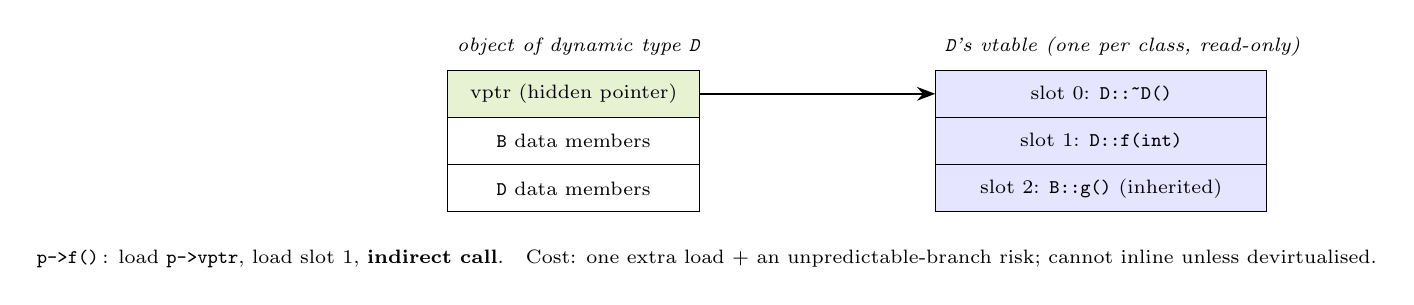
\begin{tikzpicture}[font=\scriptsize,>=Stealth,
  cell/.style={draw,minimum height=6mm,minimum width=3.2cm,anchor=west},
  lab/.style={font=\scriptsize\itshape}]
\node[lab,anchor=west] at (0,1.55) {object of dynamic type \texttt{D}};
\node[cell,fill=nvgreen!18] (vptr) at (0,0.95) {vptr (hidden pointer)};
\node[cell] (bm) at (0,0.35) {\texttt{B} data members};
\node[cell] (dm) at (0,-0.25) {\texttt{D} data members};
\node[lab,anchor=west] at (6.2,1.55) {\texttt{D}'s vtable (one per class, read-only)};
\node[cell,fill=blue!10,minimum width=4.2cm] (v0) at (6.2,0.95) {slot 0: \texttt{D::\textasciitilde D()}};
\node[cell,fill=blue!10,minimum width=4.2cm] (v1) at (6.2,0.35) {slot 1: \texttt{D::f(int)}};
\node[cell,fill=blue!10,minimum width=4.2cm] (v2) at (6.2,-0.25) {slot 2: \texttt{B::g()} (inherited)};
\draw[->,thick] (vptr.east) -- (v0.west);
\node[align=left,font=\scriptsize] at (3.3,-1.15) {\texttt{p->f()}\,: load \texttt{p->vptr}, load slot 1, \textbf{indirect call}.\quad Cost: one extra load + an unpredictable-branch risk; cannot inline unless devirtualised.};
\end{tikzpicture}
\end{center}
\begin{mustbox}
\begin{itemize}[nosep]
\item A class with at least one virtual function gets a hidden \textbf{vptr} in every object (8 bytes on x86-64) and one \textbf{vtable} per class. \texttt{sizeof} grows accordingly.
\item \texttt{override} makes the compiler check that you really override; \texttt{final} forbids further overriding. A \emph{pure virtual} function (\texttt{= 0}) makes the class \textbf{abstract} (cannot be instantiated); it may still have a body.
\item Overloading is resolved at compile time using the \emph{static} type; overriding is resolved at run time using the \emph{dynamic} type; \textbf{default arguments use the static type}.
\item Object slicing: copying a \texttt{Derived} into a \texttt{Base} \emph{object} (not reference/pointer) discards the derived part and the dynamic type.
\item Multiple inheritance can duplicate a shared base (the ``diamond''); \texttt{virtual} inheritance gives one shared sub-object.
\end{itemize}
\end{mustbox}
\needspace{5\baselineskip}
\begin{lstlisting}[language={[11]C++},title={Static default args, slicing, empty-base optimisation, vptr size}]
#include <iostream>
struct B { virtual void f(int x = 1) { std::cout << "B::f " << x << "\n"; } };
struct D : B { void f(int x = 2) override { std::cout << "D::f " << x << "\n"; } };
struct E1 {};                          // empty class
struct E2 { virtual void v() {} };     // polymorphic
struct E3 : E1 { int i; };             // empty base optimisation
int main() {
    B* p = new D;  p->f();             // dynamic type picks D::f, static type supplies default 1
    D d;  B& r = d;  r.f();            // same
    B b = D();     b.f();              // slicing: b is a plain B
    std::cout << sizeof(E1) << " " << sizeof(E2) << " " << sizeof(E3) << "\n";
    delete p;
}
\end{lstlisting}
\needspace{5\baselineskip}
\begin{lstlisting}[style=out,title={Answer: captured output}]
D::f 1
D::f 1
B::f 1
1 8 4
\end{lstlisting}
\textbf{Why:} the first two print \texttt{D::f 1} (virtual dispatch to \texttt{D::f}, but the default argument comes from \texttt{B}'s declaration); slicing gives \texttt{B::f 1}. An empty class occupies 1 byte (so distinct objects have distinct addresses), a vptr makes it 8, and an empty \emph{base} costs nothing.

\subsection{Overload resolution (a favourite C++ MCQ)}
Order of preference: \textbf{exact match} $>$ \textbf{promotion} (\texttt{char} or \texttt{short} to \texttt{int}; \texttt{float} to \texttt{double}) $>$ \textbf{standard conversion} (\texttt{int} to \texttt{double}; \texttt{int} to \texttt{char}) $>$ user-defined conversion $>$ ellipsis. Two equally good candidates $\Rightarrow$ \emph{ambiguous} (a compile error).
\needspace{5\baselineskip}
\begin{lstlisting}[language={[11]C++},title={Which overload is called?}]
#include <iostream>
void f(int)         { std::cout << "int, "; }
void f(long)        { std::cout << "long, "; }
void f(double)      { std::cout << "double, "; }
void f(const char*) { std::cout << "const char*, "; }
void g(char) { std::cout << "g(char), "; }
void g(int)  { std::cout << "g(int), "; }
int main() {
    f(1); f(1L); f(1.0f); f(nullptr); f('a'); f(0);
    g('a'); g(97);
    std::cout << "\n";
}
\end{lstlisting}
\needspace{5\baselineskip}
\begin{lstlisting}[style=out,title={Answer: captured output}]
int, long, double, const char*, int, int, g(char), g(int), 
\end{lstlisting}
\textbf{Why:} \texttt{1.0f} is \emph{promoted} to \texttt{double} (better than converting to \texttt{int}/\texttt{long}); \texttt{'a'} is promoted to \texttt{int}; \texttt{nullptr} can only become \texttt{const char*}. Now a call that \emph{looks} fine but is ambiguous:
\needspace{5\baselineskip}
\begin{lstlisting}[language={[11]C++},title={g(3.5): double converts equally well to char and to int}]
void g(char) {}
void g(int)  {}
int main() { g(3.5); }
\end{lstlisting}
\begin{lstlisting}[style=out]
prog.cpp: In function 'int main()':
prog.cpp:3:15: error: call of overloaded 'g(double)' is ambiguous
    3 | int main() { g(3.5); }
      |              ~^~~~~
prog.cpp:1:6: note: candidate: 'void g(char)'
... (5 more lines)
\end{lstlisting}


\section{Rule of 0/3/5, copy vs.\ move, and why \texttt{noexcept} matters \prio{3}}
\begin{mustbox}[The rules]
\begin{itemize}[nosep]
\item \textbf{Rule of 3:} if a class needs a custom destructor, copy constructor or copy assignment (it owns a resource), it almost certainly needs all three.
\item \textbf{Rule of 5:} add the \textbf{move constructor} and \textbf{move assignment}. \textbf{Rule of 0:} prefer members that already manage themselves (\texttt{std::vector}, \texttt{std::string}, \texttt{std::unique\_ptr}) so you write none of the five.
\item \textbf{Deep copy} duplicates the owned resource; the compiler-generated (\emph{shallow}) copy copies the pointer, causing a double \texttt{delete}.
\item \texttt{std::move(x)} is just a cast to \texttt{T\&\&}; it moves nothing by itself. The move constructor does the stealing and must leave the source valid.
\item Containers like \texttt{std::vector} move elements on reallocation \emph{only if the move constructor is \texttt{noexcept}} (otherwise they copy, to keep the strong exception guarantee).
\end{itemize}
\end{mustbox}
\needspace{5\baselineskip}
\begin{lstlisting}[language={[11]C++},title={A resource-owning class with copy-and-swap assignment}]
#include <iostream>
#include <algorithm>
#include <utility>
class Buffer {
    size_t n_; int* p_;
public:
    explicit Buffer(size_t n) : n_(n), p_(n ? new int[n]() : nullptr) { std::cout << "ctor(" << n_ << ") "; }
    Buffer(const Buffer& o) : n_(o.n_), p_(o.n_ ? new int[o.n_] : nullptr) {      // deep copy
        std::copy(o.p_, o.p_ + n_, p_); std::cout << "copy "; }
    Buffer(Buffer&& o) noexcept : n_(o.n_), p_(o.p_) { o.n_ = 0; o.p_ = nullptr; std::cout << "move "; }
    Buffer& operator=(Buffer o) noexcept { swap(o); std::cout << "assign "; return *this; }   // by value: handles copy AND move
    ~Buffer() { delete[] p_; std::cout << "dtor "; }
    void swap(Buffer& o) noexcept { std::swap(n_, o.n_); std::swap(p_, o.p_); }
    size_t size() const { return n_; }
};
int main() {
    Buffer a(3);            // ctor(3)
    Buffer b = a;           // copy
    Buffer c = std::move(a);// move; a is now empty
    b = c;                  // copy into parameter, swap, parameter dies
    c = Buffer(5);          // temporary, swap, old c data dies
    std::cout << "\nsizes: " << a.size() << b.size() << c.size() << "\n";
}   // c, b, a destroyed
\end{lstlisting}
\needspace{5\baselineskip}
\begin{lstlisting}[style=out,title={Answer: captured output}]
ctor(3) copy move copy assign dtor ctor(5) assign dtor 
sizes: 035
dtor dtor dtor 
\end{lstlisting}
\begin{qn}Why does this vector copy its elements on growth although a move constructor exists?\end{qn}
\needspace{5\baselineskip}
\begin{lstlisting}[language={[11]C++},title={vector reallocation: move vs copy (and capacity growth)}]
#include <iostream>
#include <vector>
struct X1 { X1(){} X1(const X1&){ std::cout<<"copy "; } X1(X1&&)          { std::cout<<"move "; } };
struct X2 { X2(){} X2(const X2&){ std::cout<<"copy "; } X2(X2&&) noexcept { std::cout<<"move "; } };
template<class T> void run(const char* name) {
    std::cout << name << ": ";
    std::vector<T> v;
    for (int i = 0; i < 4; i++) { v.push_back(T()); std::cout << "| "; }
    std::cout << "\n";
}
int main() {
    run<X1>("move not noexcept");
    run<X2>("move noexcept    ");
    std::vector<int> v; size_t last = 0;
    for (int i = 0; i < 20; i++) { v.push_back(i); if (v.capacity() != last) { last = v.capacity(); std::cout << last << " "; } }
    std::cout << "(capacity growth in libstdc++: doubles)\n";
}
\end{lstlisting}
\needspace{5\baselineskip}
\begin{lstlisting}[style=out,title={Answer: captured output}]
move not noexcept: move | move copy | move copy copy | move | 
move noexcept    : move | move move | move move move | move | 
1 2 4 8 16 32 (capacity growth in libstdc++: doubles)
\end{lstlisting}
\textbf{Why:} \texttt{push\_back} may reallocate (copy/move all old elements). To keep the \emph{strong} exception guarantee it uses \texttt{std::move\_if\_noexcept}: if the move constructor can throw, it copies. Mark move operations \texttt{noexcept}. (Capacity growth is implementation-defined: libstdc++ and libc++ double; MSVC grows by 1.5$\times$.)

\section{RAII and smart pointers \prio{3}}
\begin{mustbox}[RAII = Resource Acquisition Is Initialisation]
Acquire the resource in a constructor; release it in the destructor. Because destructors of fully constructed locals run on \emph{every} exit path (return, \texttt{break}, exception), leaks become structurally impossible. Examples: \texttt{std::unique\_ptr}, \texttt{std::shared\_ptr}, \texttt{std::lock\_guard}, \texttt{std::fstream}, \texttt{std::vector}.
\end{mustbox}
\begin{center}\small
\begin{tabularx}{\textwidth}{@{}L{3.2cm}Y@{}}
\toprule
\textbf{Type} & \textbf{Semantics}\\
\midrule
\texttt{unique\_ptr<T>} & Sole ownership, move-only, zero overhead over a raw pointer; custom deleters supported; first choice\\
\texttt{shared\_ptr<T>} & Shared ownership via a \textbf{control block} (strong count, weak count, deleter); atomic reference counts; \texttt{make\_shared} allocates object+block together\\
\texttt{weak\_ptr<T>} & Non-owning observer of a \texttt{shared\_ptr}; \texttt{lock()} gives a \texttt{shared\_ptr} or empty; \textbf{breaks ownership cycles}\\
raw pointer / reference & Non-owning view; never \texttt{delete} through it\\
\bottomrule
\end{tabularx}
\end{center}
\needspace{5\baselineskip}
\begin{lstlisting}[language={[11]C++},title={shared\_ptr cycle leaks; weak\_ptr back-reference fixes it}]
#include <iostream>
#include <memory>
struct N {
    std::shared_ptr<N> next;   // owning
    std::weak_ptr<N>   back;   // non-owning
    const char* n;
    N(const char* n) : n(n) {}
    ~N() { std::cout << "~" << n << " "; }
};
int main() {
    {   auto a = std::make_shared<N>("a1"), b = std::make_shared<N>("b1");
        a->next = b; b->next = a;                           // cycle: counts never reach 0
        std::cout << "cycle: use_count(a)=" << a.use_count() << "\n"; }
    std::cout << "[after cycle scope: no destructor ran -> memory leak]\n";
    {   auto a = std::make_shared<N>("a2"), b = std::make_shared<N>("b2");
        a->next = b; b->back = a;                           // weak back edge
        std::cout << "weak: use_count(a)=" << a.use_count() << " use_count(b)=" << b.use_count() << "\n"; }
    std::cout << "[after weak scope]\n";
    auto u = std::make_unique<int>(7);
    auto v = std::move(u);                                   // unique_ptr is move-only
    std::cout << (u == nullptr) << " " << *v << "\n";
}
\end{lstlisting}
\needspace{5\baselineskip}
\begin{lstlisting}[style=out,title={Answer: captured output}]
cycle: use_count(a)=2
[after cycle scope: no destructor ran -> memory leak]
weak: use_count(a)=1 use_count(b)=2
~a2 ~b2 [after weak scope]
1 7
\end{lstlisting}
\needspace{5\baselineskip}
\begin{lstlisting}[language={[11]C++},title={Copying a unique\_ptr does not compile (by design)}]
#include <memory>
int main() { std::unique_ptr<int> a(new int(1)); std::unique_ptr<int> b = a; }
\end{lstlisting}
\begin{lstlisting}[style=out]
prog.cpp: In function 'int main()':
prog.cpp:2:75: error: use of deleted function 'std::unique_ptr<_Tp, _Dp>::unique_ptr(const std::unique_ptr<_Tp, _Dp>&) [with _Tp = int; _Dp = std::default_delete<int>]'
    2 | int main() { std::unique_ptr<int> a(new int(1)); std::unique_ptr<int> b = a; }
      |                                                                           ^
... (5 more lines)
\end{lstlisting}

\begin{trapbox}[Smart-pointer pitfalls]
\begin{itemize}[nosep]
\item Never build two \texttt{shared\_ptr}s from the same raw pointer (two control blocks $\Rightarrow$ double free); copy the \texttt{shared\_ptr} or use \texttt{enable\_shared\_from\_this}.
\item \texttt{new[]} must be matched with \texttt{delete[]} (use \texttt{unique\_ptr<T[]>} or \texttt{std::vector}); mixing \texttt{malloc/delete} or \texttt{new/free} is undefined.
\item Prefer \texttt{make\_unique}/\texttt{make\_shared}: single allocation for the latter, and exception-safe argument evaluation.
\item Passing \texttt{const shared\_ptr<T>\&} costs nothing; passing by value does an atomic increment.
\end{itemize}
\end{trapbox}


% ===== 05b-cpp-more.tex.in =====
\section{Operator overloading and a ``write a class'' answer \prio{3}}
S24 reports: \emph{``Write a C++ class with operator overloading and a copy constructor.''} A model answer touches: constructors, rule of 3/5 if it owns memory, \texttt{const}-correctness, member vs.\ non-member operators, and returning the right type from each operator.
\needspace{5\baselineskip}
\begin{lstlisting}[language={[11]C++},title={Vec2: value type with overloaded operators}]
#include <iostream>
#include <stdexcept>
class Vec2 {
    double x_, y_;
public:
    Vec2(double x = 0, double y = 0) : x_(x), y_(y) {}             // default + converting ctor
    Vec2(const Vec2&) = default;                                     // rule of 0: members are trivially copyable
    double operator[](int i) const { if (i < 0 || i > 1) throw std::out_of_range("Vec2"); return i ? y_ : x_; }
    double& operator[](int i)      { if (i < 0 || i > 1) throw std::out_of_range("Vec2"); return i ? y_ : x_; }
    Vec2& operator+=(const Vec2& o) { x_ += o.x_; y_ += o.y_; return *this; }   // member: modifies *this
    Vec2& operator++()    { ++x_; ++y_; return *this; }              // prefix: returns the NEW value by reference
    Vec2  operator++(int) { Vec2 old = *this; ++*this; return old; } // postfix: dummy int, returns the OLD value by value
    friend Vec2 operator+(Vec2 a, const Vec2& b) { return a += b; }  // non-member: symmetric conversions
    friend bool operator==(const Vec2& a, const Vec2& b) { return a.x_ == b.x_ && a.y_ == b.y_; }
    friend std::ostream& operator<<(std::ostream& os, const Vec2& v) { return os << "(" << v.x_ << "," << v.y_ << ")"; }
};
int main() {
    Vec2 a(1, 2), b(3, 4);
    Vec2 c = a + b;                       // copy-initialisation from the returned temporary
    Vec2 d(c);                            // copy constructor
    std::cout << c << " " << (c == d) << " " << c[1] << "\n";
    std::cout << c++ << " " << c << " " << ++c << "\n";
    try { c[2]; } catch (const std::out_of_range& e) { std::cout << "caught " << e.what() << "\n"; }
}
\end{lstlisting}
\needspace{5\baselineskip}
\begin{lstlisting}[style=out,title={Answer: captured output}]
(4,6) 1 6
(4,6) (5,7) (6,8)
caught Vec2
\end{lstlisting}
\begin{mustbox}[Operator-overloading rules]
\begin{itemize}[nosep]
\item Cannot be overloaded: \texttt{::}, \texttt{.}, \texttt{.*}, \texttt{?:}, \texttt{sizeof}. Cannot invent new operators. At least one operand must be a user-defined type.
\item \texttt{=}, \texttt{[]}, \texttt{()}, \texttt{->} must be \emph{member} functions; \texttt{<<}/\texttt{>>} for streams must be non-members (the left operand is the stream).
\item Prefix \texttt{++} returns \texttt{T\&}; postfix \texttt{++(int)} returns \texttt{T} by value (and is slower for heavy types: prefer \texttt{++it}).
\item Keep the usual semantics: \texttt{+} returns a new value, \texttt{+=} modifies and returns \texttt{*this}; if you define \texttt{==}, define \texttt{!=} (automatic in C++20) and keep them consistent.
\end{itemize}
\end{mustbox}

\section{Diamond inheritance and virtual bases \prio{2}}
\needspace{5\baselineskip}
\begin{lstlisting}[language={[11]C++},title={Two copies of A vs. one shared A}]
#include <iostream>
struct A  { A()  { std::cout << "A "; } };
struct B1 : A { B1() { std::cout << "B "; } };
struct C1 : A { C1() { std::cout << "C "; } };
struct D1 : B1, C1 { D1() { std::cout << "D | "; } };      // contains TWO A sub-objects
struct VB : virtual A { VB() { std::cout << "B "; } };
struct VC : virtual A { VC() { std::cout << "C "; } };
struct VD : VB, VC { VD() { std::cout << "D"; } };         // ONE shared A, built first by the most-derived class
int main() { D1 d1; VD vd; std::cout << "\n"; std::cout << sizeof(D1) << " " << sizeof(VD) << "\n"; }
\end{lstlisting}
\needspace{5\baselineskip}
\begin{lstlisting}[style=out,title={Answer: captured output}]
A B A C D | A B C D
2 16
\end{lstlisting}
\textbf{Why:} without \texttt{virtual}, \texttt{D1} has two \texttt{A} bases (ambiguous member access, double construction); with virtual inheritance the \emph{most derived} class constructs the single \texttt{A} first. Virtual bases cost extra pointers (hence the bigger \texttt{VD}).

\section{Templates \prio{3}}
\begin{mustbox}
\begin{itemize}[nosep]
\item Templates are \textbf{compile-time generics}: the compiler instantiates a separate function/class for each distinct set of template arguments. Consequences: header-only definitions, longer compile times, possible code bloat, and errors reported at instantiation.
\item \textbf{Specialisation:} \emph{full} (\texttt{template<>} followed by the specialised declaration) for one exact type; \emph{partial} (classes only) for a family (e.g.\ \texttt{T*}). Function templates cannot be partially specialised: use overloading.
\item \textbf{Deduction} takes the argument types: \texttt{max(1, 2.5)} fails to deduce one \texttt{T}; write \texttt{max<double>(1, 2.5)}.
\item \textbf{SFINAE} (``substitution failure is not an error''), \texttt{if constexpr} (C++17) and \textbf{concepts} (C++20) select code by type properties. \texttt{typename} marks a dependent type name.
\item \textbf{Variadic templates} + \textbf{fold expressions} (C++17): \texttt{(args + ...)}. \textbf{CRTP}: a class derives from \texttt{Base<Derived>} to get static (zero-cost) polymorphism.
\end{itemize}
\end{mustbox}
\needspace{5\baselineskip}
\begin{lstlisting}[language={[11]C++},title={Specialisation, variadic/fold, if constexpr, SFINAE, constexpr}]
#include <iostream>
#include <string>
#include <type_traits>
template <typename T> T maxof(T a, T b) { return a > b ? a : b; }
template <> const char* maxof<const char*>(const char* a, const char* b) {      // full specialisation
    return std::string(a) > std::string(b) ? a : b; }                           // (a > b on raw pointers would compare ADDRESSES)
template <typename T> struct Describe { static const char* name() { return "other"; } };
template <typename T> struct Describe<T*> { static const char* name() { return "pointer"; } };   // partial
template <> struct Describe<int> { static const char* name() { return "int"; } };               // full
template <typename... Ts> auto fold_sum(Ts... ts) { return (ts + ...); }                         // C++17 fold
template <typename T> const char* kind(T) {
    if constexpr (std::is_integral_v<T>) return "integral";           // discarded branch is not instantiated
    else if constexpr (std::is_floating_point_v<T>) return "floating";
    else return "other";
}
template <typename T> std::enable_if_t<std::is_integral_v<T>, T> half(T v) { return v / 2; }    // SFINAE: only integers
template <int N> struct Fact { static constexpr long long value = N * Fact<N - 1>::value; };   // template metaprogramming
template <> struct Fact<0> { static constexpr long long value = 1; };
constexpr long long fact(int n) { return n <= 1 ? 1 : n * fact(n - 1); }                       // constexpr function
static_assert(fact(5) == 120 && Fact<5>::value == 120, "evaluated at compile time");
template <class D> struct Shape { double area() const { return static_cast<const D*>(this)->area_impl(); } };   // CRTP
struct Sq : Shape<Sq> { double s; explicit Sq(double s) : s(s) {} double area_impl() const { return s * s; } };
int main() {
    std::cout << maxof(3, 7) << " " << maxof(2.5, 1.5) << " " << maxof<const char*>("pear", "apple") << "\n";
    std::cout << Describe<double>::name() << " " << Describe<char*>::name() << " " << Describe<int>::name() << "\n";
    std::cout << fold_sum(1, 2, 3, 4) << " " << fold_sum(1.5, 2.5) << " " << kind(7) << " " << kind(2.0) << " " << kind("x") << "\n";
    std::cout << half(9) << " " << Fact<10>::value << " " << Sq(3).area() << "\n";
}
\end{lstlisting}
\needspace{5\baselineskip}
\begin{lstlisting}[style=out,title={Answer: captured output}]
7 2.5 pear
other pointer int
10 4 integral floating other
4 3628800 9
\end{lstlisting}
\needspace{5\baselineskip}
\begin{lstlisting}[language={[11]C++},title={max(1, 2.5): conflicting deduction}]
template <typename T> T maxof(T a, T b) { return a > b ? a : b; }
int main() { return (int)maxof(1, 2.5); }
\end{lstlisting}
\begin{lstlisting}[style=out]
prog.cpp: In function 'int main()':
prog.cpp:2:31: error: no matching function for call to 'maxof(int, double)'
    2 | int main() { return (int)maxof(1, 2.5); }
      |                          ~~~~~^~~~~~~~
... (7 more lines)
\end{lstlisting}

\begin{tipbox}[Templates vs.\ macros vs.\ \texttt{inline} (S22 asked about templates and inline functions)]
\textbf{Macro:} text substitution, no types, double evaluation. \textbf{\texttt{inline} function:} ordinary typed function whose body the compiler \emph{may} inline; \texttt{inline} also relaxes the one-definition rule so the definition can live in a header. \textbf{Template:} a family of functions/classes generated per type. Inlining is a compiler decision; the keyword is only a hint.
\end{tipbox}

\section{The STL: containers, complexities, iterator invalidation \prio{3}}
\begin{center}\small
\begin{tabularx}{\textwidth}{@{}L{3.1cm}L{3.0cm}Y@{}}
\toprule
\textbf{Container} & \textbf{Access / find} & \textbf{Insert / erase (and notes)}\\
\midrule
\texttt{vector} & $O(1)$ index; $O(n)$ find & push\_back amortised $O(1)$; middle $O(n)$; contiguous (cache-friendly)\\
\texttt{deque} & $O(1)$ index & push/pop at both ends $O(1)$; middle $O(n)$; not contiguous\\
\texttt{list} / \texttt{forward\_list} & $O(n)$ & $O(1)$ at a known iterator; node-based, poor locality; splice $O(1)$\\
\texttt{array<T,N>} & $O(1)$ & fixed size, no heap\\
\texttt{set} / \texttt{map} (+multi) & $O(\log n)$ & $O(\log n)$; red-black tree; sorted iteration; \texttt{map[]} \textbf{inserts} a default value\\
\texttt{unordered\_set/map} & average $O(1)$, worst $O(n)$ & hash table; rehash invalidates iterators; needs \texttt{hash} and \texttt{==}\\
\texttt{priority\_queue} & top $O(1)$ & push/pop $O(\log n)$; max-heap by default (\texttt{greater<>} gives min-heap)\\
\texttt{stack}, \texttt{queue} & & adaptors over \texttt{deque}/\texttt{vector}\\
\texttt{bitset<N>} & $O(1)$ bit access & fixed size; fast bulk bit ops\\
\bottomrule
\end{tabularx}
\end{center}
\begin{center}\small
\begin{tabularx}{\textwidth}{@{}L{4.3cm}Y@{}}
\toprule
\textbf{Algorithm} & \textbf{Complexity / contract}\\
\midrule
\texttt{sort} & $O(n\log n)$ (introsort); needs random access and a \textbf{strict weak ordering} (\texttt{<}, never \texttt{<=}: that is UB and can crash)\\
\texttt{stable\_sort}, \texttt{partial\_sort}, \texttt{nth\_element} & $O(n\log n)$ stable; $O(n\log k)$; $O(n)$ average\\
\texttt{lower\_bound}, \texttt{upper\_bound}, \texttt{binary\_search} & $O(\log n)$ on a \emph{sorted} range; first $\ge$ / first $>$ the key\\
\texttt{unique}, \texttt{remove}, \texttt{remove\_if} & \textbf{do not shrink} the container: they return the new logical end; use the \emph{erase--remove idiom}\\
\texttt{accumulate}, \texttt{iota}, \texttt{next\_permutation}, \texttt{reverse}, \texttt{rotate} & $O(n)$; \texttt{next\_permutation} yields all $n!$ orders if you start sorted\\
\bottomrule
\end{tabularx}
\end{center}
\begin{trapbox}[Iterator invalidation (classic MCQ)]
\textbf{vector:} \texttt{push\_back} invalidates \emph{all} iterators/references if it reallocates (capacity exceeded), otherwise only \texttt{end()}; \texttt{insert/erase} invalidate everything at/after the position. \textbf{deque:} insert in the middle invalidates all; at the ends it invalidates iterators but not references. \textbf{list/set/map:} only iterators to erased elements. \textbf{unordered containers:} a rehash invalidates all iterators (references/pointers to elements stay valid).
Erasing while looping: \texttt{it = c.erase(it)} (it returns the next iterator), never \texttt{c.erase(it); ++it}.
\end{trapbox}
\needspace{5\baselineskip}
\begin{lstlisting}[language={[11]C++},title={STL idioms: erase-remove, bounds, map[], heap, string search}]
#include <algorithm>
#include <functional>
#include <iostream>
#include <map>
#include <numeric>
#include <queue>
#include <string>
#include <vector>
using namespace std;
int main() {
    vector<int> v{5, 2, 8, 2, 9, 1, 5};
    sort(v.begin(), v.end());
    v.erase(unique(v.begin(), v.end()), v.end());                    // sort + unique + erase = distinct values
    for (int x : v) cout << x << ' ';  cout << "| ";
    cout << *lower_bound(v.begin(), v.end(), 5) << " " << *upper_bound(v.begin(), v.end(), 5) << " | ";
    v.erase(remove_if(v.begin(), v.end(), [](int x) { return x % 2 == 0; }), v.end());   // erase-remove idiom
    for (int x : v) cout << x << ' ';  cout << "\n";
    map<string, int> m;  m["a"]++;  m["b"] += 2;
    cout << m.size() << " " << m["zzz"] << " " << m.size() << " " << m.count("q") << " " << m.size() << "\n";   // operator[] inserts
    priority_queue<int, vector<int>, greater<int>> pq;                // min-heap
    for (int x : {5, 1, 4, 2, 3}) pq.push(x);
    while (!pq.empty()) { cout << pq.top() << ' '; pq.pop(); }
    cout << "| ";
    vector<int> w(5); iota(w.begin(), w.end(), 1);                    // 1 2 3 4 5
    cout << accumulate(w.begin(), w.end(), 0) << " " << accumulate(w.begin(), w.end(), 1, multiplies<int>()) << " | ";
    string s = "compiler verification";
    cout << s.find("ver") << " " << (s.find("xyz") == string::npos) << " " << s.substr(0, 8) << "\n";
    vector<int> p{1, 2, 3}; int cnt = 0;
    do { cnt++; } while (next_permutation(p.begin(), p.end()));
    cout << cnt << " permutations\n";
}
\end{lstlisting}
\needspace{5\baselineskip}
\begin{lstlisting}[style=out,title={Answer: captured output}]
1 2 5 8 9 | 5 8 | 1 5 9 
2 0 3 0 3
1 2 3 4 5 | 15 120 | 9 1 compiler
6 permutations
\end{lstlisting}
\textbf{Why (map line):} \texttt{m.size()} is 2; \texttt{m["zzz"]} silently inserts a zero entry (size 3); \texttt{count} does not insert. Use \texttt{find} or \texttt{at} (throws) to look up without inserting.

\section{Lambdas, \texttt{auto}, casts and const-correctness \prio{2}}
\needspace{5\baselineskip}
\begin{lstlisting}[language={[11]C++},title={Lambda captures; auto deduction}]
#include <iostream>
#include <type_traits>
#include <vector>
#include <algorithm>
int main() {
    int x = 10;
    auto by_val = [x]() mutable { x++; return x; };     // copy captured at creation; mutable lets us modify the copy
    auto by_ref = [&x]() { x++; return x; };            // reference: sees and changes the original
    std::cout << by_val() << " " << by_val() << " " << x << " " << by_ref() << " " << x << "\n";
    const int& r = x;
    auto a = r;                                          // auto drops const and reference -> int
    auto& b = r;                                         // keeps const -> const int&
    std::cout << std::is_same_v<decltype(a), int> << std::is_same_v<decltype(b), const int&> << "\n";
    auto l = {1, 2, 3};                                  // std::initializer_list<int>
    std::cout << std::is_same_v<decltype(l), std::initializer_list<int>> << "\n";
    std::vector<std::pair<int,int>> pts{{3, 1}, {1, 2}, {2, 0}};
    std::sort(pts.begin(), pts.end(), [](const auto& p, const auto& q) { return p.second < q.second; });   // generic lambda as comparator
    for (auto& [a1, b1] : pts) std::cout << a1 << ':' << b1 << ' ';                             // structured bindings
    std::cout << "\n";
}
\end{lstlisting}
\needspace{5\baselineskip}
\begin{lstlisting}[style=out,title={Answer: captured output}]
11 12 10 11 11
11
1
2:0 3:1 1:2 
\end{lstlisting}
\begin{mustbox}[Casts and const-correctness]
\begin{itemize}[nosep]
\item \texttt{static\_cast}: well-defined conversions between related types (numeric, up/down a hierarchy without checking). \texttt{dynamic\_cast}: checked down/cross-casts of \emph{polymorphic} types (needs RTTI; returns \texttt{nullptr} or throws \texttt{bad\_cast}). \texttt{const\_cast}: adds/removes \texttt{const}; \emph{modifying} a truly const object through it is UB. \texttt{reinterpret\_cast}: reinterpret bits (pointer$\leftrightarrow$integer); legal only in narrow cases. C-style \texttt{(T)x} tries all of them: avoid.
\item A \texttt{const} member function promises not to change observable state; \texttt{mutable} members (caches, mutexes) are the exception. Overload on \texttt{const} to give \texttt{const} and non-\texttt{const} access (see \texttt{Vec2::operator[]}).
\item \texttt{explicit} stops implicit conversions through single-argument constructors and conversion operators. Brace initialisation forbids narrowing: \texttt{int a\{3.5\};} does not compile.
\item \textbf{Value categories:} lvalue (has identity, can take its address), prvalue (a pure temporary), xvalue (an expiring object, e.g.\ \texttt{std::move(x)}); \texttt{T\&\&} binds to rvalues; in a template, \texttt{T\&\&} is a \emph{forwarding reference}, and \texttt{std::forward<T>} preserves the category (``perfect forwarding'').
\end{itemize}
\end{mustbox}

\section{Exceptions and stack unwinding \prio{2}}
\needspace{5\baselineskip}
\begin{lstlisting}[language={[11]C++},title={Destructors run during unwinding, in reverse order}]
#include <iostream>
#include <stdexcept>
struct G { const char* n; G(const char* n) : n(n) { std::cout << "+" << n << " "; } ~G() { std::cout << "-" << n << " "; } };
void f() { G a("a"); throw std::runtime_error("boom"); }
int main() {
    try { G b("b"); f(); std::cout << "not reached "; }
    catch (const std::exception& e) { std::cout << "caught " << e.what() << "\n"; }
}
\end{lstlisting}
\needspace{5\baselineskip}
\begin{lstlisting}[style=out,title={Answer: captured output}]
+b +a -a -b caught boom
\end{lstlisting}
\begin{mustbox}
Throw by value, catch by (const) reference. Handlers are tried in order, so put \emph{derived} types before bases. \textbf{Destructors must not throw} (they are \texttt{noexcept} by default; throwing during unwinding calls \texttt{std::terminate}). Exception-safety levels: \emph{basic} (no leaks, valid state), \emph{strong} (commit-or-rollback), \emph{no-throw}. Exceptions cost nothing on the non-throwing path in modern ABIs (table-based unwinding) but are slow when thrown; GPU device code (CUDA) does not support them.
\end{mustbox}

\section{Undefined behaviour, ODR and initialisation order in C++ \prio{3}}
\begin{center}\small
\begin{tabularx}{\textwidth}{@{}L{5.4cm}Y@{}}
\toprule
\textbf{C++ undefined behaviour} & \textbf{Typical real-world symptom}\\
\midrule
Signed overflow, out-of-range shifts, divide by zero & Surprising optimisation (see Chapter~\ref{ch:c}); SIGFPE\\
Out-of-bounds \texttt{v[i]} (no check), \texttt{front()} of an empty container & Silent corruption; use \texttt{at()} or \texttt{-D\_GLIBCXX\_ASSERTIONS} to trap\\
Using an invalidated iterator, dangling reference, reference to a destroyed temporary & Garbage values, crashes far from the bug\\
\texttt{delete} of a base pointer without virtual destructor; \texttt{delete} vs.\ \texttt{delete[]} mismatch & Leaks, heap corruption\\
Reading an inactive union member (type punning other than via \texttt{memcpy}/\texttt{bit\_cast}) & Compiler may assume the other member is untouched\\
Data race on a non-atomic object; modifying a \texttt{const} object; violating \texttt{restrict}/aliasing rules & Impossible-looking behaviour at \texttt{-O2}\\
\textbf{ODR violation:} two different definitions of the same entity in different translation units & Link succeeds; wrong function is silently picked\\
Missing return in a non-void function (C++) & Falls off the end: UB (unlike \texttt{main})\\
\bottomrule
\end{tabularx}
\end{center}
\begin{trapbox}[Static initialisation order fiasco]
Within one translation unit globals are initialised in definition order; \textbf{across translation units the order is unspecified}. A global in \texttt{a.cpp} that uses a global from \texttt{b.cpp} in its constructor may see it uninitialised. Fix: a function-local \texttt{static} (the ``construct on first use'' idiom), initialised thread-safely on first call. Function-local statics are initialised once, the first time control passes through them.
\end{trapbox}
\needspace{5\baselineskip}
\begin{lstlisting}[language={[11]C++},title={Initialisation order within one translation unit}]
#include <iostream>
struct S { S(const char* n) { std::cout << "init " << n << "\n"; } };
S a("a");  static S b("b");
void f() { static S c("c"); }                 // initialised once, on first call
int main() { std::cout << "main start\n"; f(); f(); S d("d"); std::cout << "main end\n"; }
S z("z");                                      // defined later in the file, still before main
\end{lstlisting}
\needspace{5\baselineskip}
\begin{lstlisting}[style=out,title={Answer: captured output}]
init a
init b
init z
main start
init c
init d
main end
\end{lstlisting}
\textbf{Why:} namespace-scope objects are constructed before \texttt{main} in definition order (\texttt{a, b, z}); \texttt{c} is constructed at the first call of \texttt{f}; \texttt{d} is an automatic.

\section{C++ output-prediction drills \prio{3}}
\begin{qn}Does \texttt{std::move} move?\end{qn}
\begin{lstlisting}[language={[11]C++}]
#include <iostream>
#include <string>
#include <utility>
int main() {
    std::string a = "hello";
    std::string b = std::move(a);                       // moves: a is valid but unspecified (empty in practice)
    const std::string c = "world";
    std::string d = std::move(c);                       // c is const: T&& cannot bind -> COPY constructor is used
    std::cout << "[" << a << "] [" << b << "] [" << c << "] [" << d << "]\n";
}
\end{lstlisting}
\needspace{5\baselineskip}
\begin{lstlisting}[style=out,title={Answer: captured output}]
[] [hello] [world] [world]
\end{lstlisting}
\textbf{Why:} \texttt{std::move} is only a cast. A moved-from \texttt{string} is typically empty. A \texttt{const} object cannot be moved from, so the copy constructor runs and \texttt{c} keeps its value.

\begin{qn}Narrowing in brace initialisation.\end{qn}
\needspace{5\baselineskip}
\begin{lstlisting}[language={[11]C++},title={int a\{3.5\}; is ill-formed}]
int main() { int a{3.5}; (void)a; }
\end{lstlisting}
\begin{lstlisting}[style=out]
(no output)
\end{lstlisting}
\textbf{Why:} brace-init forbids narrowing conversions (double to int); \texttt{int a = 3.5;} would compile (with truncation) and \texttt{int a(3.5)} too.

\begin{qn}\texttt{sizeof} of common standard types (libstdc++, x86-64).\end{qn}
\begin{lstlisting}[language={[11]C++}]
#include <iostream>
#include <memory>
#include <string>
#include <vector>
#include <map>
#include <functional>
int main() {
    std::cout << "string=" << sizeof(std::string) << " vector=" << sizeof(std::vector<int>)
              << " unique_ptr=" << sizeof(std::unique_ptr<int>) << " shared_ptr=" << sizeof(std::shared_ptr<int>)
              << " map=" << sizeof(std::map<int,int>) << " function=" << sizeof(std::function<void()>) << "\n";
}
\end{lstlisting}
\needspace{5\baselineskip}
\begin{lstlisting}[style=out,title={Answer: captured output (implementation-specific!)}]
string=32 vector=24 unique_ptr=8 shared_ptr=16 map=48 function=32
\end{lstlisting}
\textbf{Why:} \texttt{vector} = 3 pointers (begin, end, end-of-capacity); \texttt{unique\_ptr} = 1 pointer; \texttt{shared\_ptr} = object pointer + control-block pointer; \texttt{string} embeds a 15-char small buffer. Do not memorise these numbers: say ``implementation-defined'' and explain the layout.

\begin{qn}Order of \texttt{<<} evaluation and \texttt{i++}.\end{qn}
\begin{lstlisting}[language={[11]C++}]
#include <iostream>
int main() {
    int i = 1;
    std::cout << i++ << " " << i << " " << ++i << "\n";   // C++17: left-to-right for the operands of <<
}
\end{lstlisting}
\needspace{5\baselineskip}
\begin{lstlisting}[style=out,title={Answer: captured output}]
1 2 3
\end{lstlisting}
\textbf{Why:} since C++17 the operands of \texttt{<<} are sequenced left to right, so this is well defined. Before C++17 it was unspecified; the \emph{function-argument} version \texttt{f(i++, i)} is still unspecified.


% ===== 06-python.tex.in =====
\chapter{Python: Data Model, Gotchas and Automation}
\label{ch:python}

\begin{chapbox}
\textbf{Priority \prio{3}. Time: 60 min.} Python is half the job (tools, runners, parsers) and is named in the OA skills list. Expect snippet-output MCQs on mutability, scoping, comprehensions and
class behaviour, plus a coding problem. Outputs below are real (CPython 3.13); behaviour that depends on the interpreter version is flagged.
\end{chapbox}

\section{The data model: names, objects, mutability \prio{3}}
\begin{mustbox}[Four sentences that answer half of all Python MCQs]
\begin{enumerate}[nosep]
\item Variables are \textbf{names bound to objects}; assignment never copies: \texttt{b = a} makes a second name for the same object.
\item \textbf{Mutable} types (\texttt{list, dict, set, bytearray}, most user classes) change in place; \textbf{immutable} types (\texttt{int, float, str, tuple, frozenset, bytes}) never do; operations create new objects.
\item \texttt{==} compares \emph{values} (\texttt{\_\_eq\_\_}); \texttt{is} compares \emph{identity}. Use \texttt{is} only for \texttt{None}/singletons.
\item Function arguments are passed ``by object reference'': the callee gets a new name for the caller's object; rebinding it does not affect the caller, mutating it does.
\end{enumerate}
\end{mustbox}
\begin{qn}Identity, equality and the small-integer cache.\end{qn}
\begin{lstlisting}[language={Python}]
a = int("257"); b = int("257")
print(a == b, a is b)            # equal values, distinct objects
c = int("5"); d = int("5")
print(c == d, c is d)            # CPython caches the small ints -5..256 (an implementation detail)
l1, l2 = [], []
print(l1 == l2, l1 is l2)
x = None
print(x is None, x == None)      # 'is None' is the idiom
\end{lstlisting}
\needspace{5\baselineskip}
\begin{lstlisting}[style=out,title={Answer: captured output}]
True False
True True
True False
True True
\end{lstlisting}
\textbf{Why:} never rely on \texttt{is} for numbers or strings: whether two equal values share an object is an interpreter optimisation, not language semantics.

\begin{qn}The mutable default-argument trap.\end{qn}
\begin{lstlisting}[language={Python}]
def add(x, acc=[]):               # the default list is created ONCE, when def runs
    acc.append(x)
    return acc

def add_fixed(x, acc=None):
    if acc is None:
        acc = []
    acc.append(x)
    return acc

print(add(1), add(2), add(3))
print(add_fixed(1), add_fixed(2), add_fixed(3))
\end{lstlisting}
\needspace{5\baselineskip}
\begin{lstlisting}[style=out,title={Answer: captured output}]
[1, 2, 3] [1, 2, 3] [1, 2, 3]
[1] [2] [3]
\end{lstlisting}
\textbf{Why:} all three calls mutate the same list object; the three prints show it after all calls finished. Use \texttt{None} as the sentinel.

\begin{qn}Aliasing, shallow and deep copies.\end{qn}
\begin{lstlisting}[language={Python}]
import copy
g = [[0] * 3] * 3                 # three references to ONE inner list
g[0][0] = 1
print(g)
h = [[0] * 3 for _ in range(3)]   # three distinct lists
h[0][0] = 1
print(h)
a = [[1, 2], [3]]
shallow, deep = a.copy(), copy.deepcopy(a)
a[0].append(99)
print(shallow, deep)              # shallow copy shares the inner lists
\end{lstlisting}
\needspace{5\baselineskip}
\begin{lstlisting}[style=out,title={Answer: captured output}]
[[1, 0, 0], [1, 0, 0], [1, 0, 0]]
[[1, 0, 0], [0, 0, 0], [0, 0, 0]]
[[1, 2, 99], [3]] [[1, 2], [3]]
\end{lstlisting}

\begin{qn}\texttt{+=} versus \texttt{+}, and a tuple that raises but still changes.\end{qn}
\begin{lstlisting}[language={Python}]
a = [1, 2]; b = a; a += [3]       # += on a list extends IN PLACE
print(b)
a = [1, 2]; b = a; a = a + [3]    # + builds a NEW list and rebinds a
print(b)
t = ([1], 2)
try:
    t[0] += [3]                   # list.__iadd__ mutates the list, THEN tuple item assignment fails
except TypeError as e:
    print("TypeError:", e)
print(t)
\end{lstlisting}
\needspace{5\baselineskip}
\begin{lstlisting}[style=out,title={Answer: captured output}]
[1, 2, 3]
[1, 2]
TypeError: 'tuple' object does not support item assignment
([1, 3], 2)
\end{lstlisting}

\begin{qn}Late-binding closures.\end{qn}
\begin{lstlisting}[language={Python}]
fs = [lambda: i for i in range(3)]
print([f() for f in fs])          # i is looked up when the lambda RUNS, after the loop ended (i == 2)
gs = [lambda i=i: i for i in range(3)]   # default argument captures the value at definition time
print([g() for g in gs])
\end{lstlisting}
\needspace{5\baselineskip}
\begin{lstlisting}[style=out,title={Answer: captured output}]
[2, 2, 2]
[0, 1, 2]
\end{lstlisting}

\begin{qn}Scope: LEGB, \texttt{global}, \texttt{nonlocal}.\end{qn}
\begin{lstlisting}[language={Python}]
x = 10
def f():
    print("f sees", x)            # no assignment to x in f: reads the global
def g():
    try:
        print(x)                  # x is assigned below, so x is LOCAL in all of g
        x = 5
    except UnboundLocalError:
        print("UnboundLocalError")
def h():
    global x
    x += 1
def counter():
    n = 0
    def inc():
        nonlocal n                # rebind the enclosing function's variable
        n += 1
        return n
    return inc
f(); g(); h(); print(x)
c = counter(); print(c(), c(), c())
\end{lstlisting}
\needspace{5\baselineskip}
\begin{lstlisting}[style=out,title={Answer: captured output}]
f sees 10
UnboundLocalError
11
1 2 3
\end{lstlisting}
\textbf{Why:} Python decides a name's scope at compile time per function: any assignment inside makes it local unless declared \texttt{global}/\texttt{nonlocal}. Lookup order: \textbf{L}ocal, \textbf{E}nclosing, \textbf{G}lobal, \textbf{B}uilt-in.

\section{Numbers, strings and containers \prio{3}}
\begin{center}\small
\begin{tabularx}{\textwidth}{@{}L{3.2cm}L{3.4cm}L{3.4cm}Y@{}}
\toprule
\textbf{Expression} & \textbf{C / C++} & \textbf{Python} & \textbf{Reason}\\
\midrule
$-7 / 2$ & $-3$ & $-3.5$ (\texttt{-7 // 2} = $-4$) & Python \texttt{/} is true division; \texttt{//} \textbf{floors}\\
$-7 \bmod 2$ & $-1$ & $1$ & Python's result takes the sign of the \emph{divisor}\\
Integer size & 32/64-bit, overflow & arbitrary precision & big ints never overflow (but are slower)\\
\texttt{round(2.5)} & (library dependent) & 2 & banker's rounding: ties go to even\\
\bottomrule
\end{tabularx}
\end{center}
\begin{lstlisting}[language={Python}]
print(-7 // 2, -7 % 2, divmod(-7, 2), 7 // -2, 7 % -2)
print(round(2.5), round(3.5), round(-2.5), int(-2.9), 0.1 + 0.2, 0.1 + 0.2 == 0.3)
print(2 ** 100, 3 / 2, 3 // 2, 3.0 // 2, -3 // 2.0, 2 ** -1)
print(True + True, True == 1, isinstance(True, int), 1 < 2 < 3, 1 < 3 < 2)
print(0 or "a", "" or [] or None, 1 and 2, 0 and 2, not [])   # and/or return one of their OPERANDS
\end{lstlisting}
\needspace{5\baselineskip}
\begin{lstlisting}[style=out,title={Answer: captured output}]
-4 1 (-4, 1) -4 -1
2 4 -2 -2 0.30000000000000004 False
1267650600228229401496703205376 1.5 1 1.0 -2.0 0.5
2 True True True False
a None 2 0 True
\end{lstlisting}
\needspace{5\baselineskip}
\begin{lstlisting}[language={Python},title={Strings: slicing, immutability, f-strings}]
s = "compiler"
print(s[::-1], s[1:4], s[-3:], s[::2], repr(s[10:]), s.upper(), s.find("p"), s.count("e"))
print(",".join(["a", "b"]), "a b  c".split(), "a,b,,c".split(","), "  x ".strip() + "|")
print(f"{3.14159:.2f} {42:05d} {255:#x} {'x':>4} {1234567:,}")
try:
    s[0] = "C"
except TypeError as e:
    print("TypeError:", e)
\end{lstlisting}
\needspace{5\baselineskip}
\begin{lstlisting}[style=out,title={Answer: captured output}]
relipmoc omp ler cmie '' COMPILER 3 1
a,b ['a', 'b', 'c'] ['a', 'b', '', 'c'] x|
3.14 00042 0xff    x 1,234,567
TypeError: 'str' object does not support item assignment
\end{lstlisting}
\needspace{5\baselineskip}
\begin{lstlisting}[language={Python},title={Containers: dict, set, Counter, deque, defaultdict}]
from collections import Counter, defaultdict, deque
c = Counter("mississippi")
print(c.most_common(2), c["z"])
d = defaultdict(list); d["a"].append(1); d["a"].append(2); print(dict(d))
dq = deque([1, 2, 3]); dq.appendleft(0); dq.rotate(1); print(dq)
st = {1, 2, 3}
print(st & {2, 3, 4}, st | {4}, st - {1}, st ^ {3, 4})
try:
    {[1]: 2}
except TypeError as e:
    print("TypeError:", e)
words = ["bb", "a", "ccc", "dd"]
print(sorted(words, key=len), sorted(words, key=lambda w: (-len(w), w)))   # sort is stable
r = words.sort()
print(r, words)                                                            # list.sort() returns None
\end{lstlisting}
\needspace{5\baselineskip}
\begin{lstlisting}[style=out,title={Answer: captured output}]
[('i', 4), ('s', 4)] 0
{'a': [1, 2]}
deque([3, 0, 1, 2])
{2, 3} {1, 2, 3, 4} {2, 3} {1, 2, 4}
TypeError: unhashable type: 'list'
['a', 'bb', 'dd', 'ccc'] ['ccc', 'bb', 'dd', 'a']
None ['a', 'bb', 'ccc', 'dd']
\end{lstlisting}
\begin{tipbox}[Complexity cheat-sheet (CPython)]
\texttt{list}: index $O(1)$, append amortised $O(1)$, \texttt{insert(0,x)}/\texttt{pop(0)}/\texttt{x in list} $O(n)$. \texttt{deque}: both ends $O(1)$. \texttt{dict}/\texttt{set}: average $O(1)$ get/set/\texttt{in}. \texttt{str += str} in a loop is $O(n^2)$ in the worst case; build a list and \texttt{"".join}. \texttt{sorted} is Timsort, $O(n\log n)$, stable. \texttt{heapq} is a min-heap (negate for max-heap); \texttt{bisect} does binary search on sorted lists.
\end{tipbox}

\section{Iterators, generators and the standard toolbox \prio{3}}
\begin{lstlisting}[language={Python}]
from itertools import islice, accumulate, groupby, permutations, combinations, product
g = (x * x for x in range(4))
print(list(g), list(g))                    # a generator is exhausted after one pass
def fib():
    a, b = 0, 1
    while True:
        yield a                            # suspends here, keeps local state
        a, b = b, a + b
print(list(islice(fib(), 10)))
print(list(accumulate([1, 2, 3, 4])), list(combinations("abc", 2)), len(list(permutations(range(4)))))
print(list(product("ab", repeat=2)), list(zip([1, 2, 3], "ab")), [k for k, _ in groupby("aabbbc")])
print(list(map(lambda x: x * 2, [1, 2])), [x for x in range(10) if x % 3 == 0], {x: x * x for x in range(3)})
\end{lstlisting}
\needspace{5\baselineskip}
\begin{lstlisting}[style=out,title={Answer: captured output}]
[0, 1, 4, 9] []
[0, 1, 1, 2, 3, 5, 8, 13, 21, 34]
[1, 3, 6, 10] [('a', 'b'), ('a', 'c'), ('b', 'c')] 24
[('a', 'a'), ('a', 'b'), ('b', 'a'), ('b', 'b')] [(1, 'a'), (2, 'b')] ['a', 'b', 'c']
[2, 4] [0, 3, 6, 9] {0: 0, 1: 1, 2: 4}
\end{lstlisting}
\begin{mustbox}
\texttt{map}, \texttt{filter}, \texttt{zip}, \texttt{range}, \texttt{enumerate} return lazy iterators in Python 3. \texttt{zip} stops at the shortest input. A comprehension has its own scope (the loop variable does not leak in Python 3). \texttt{for/else}: the \texttt{else} block runs if the loop was \emph{not} ended by \texttt{break}. \texttt{try/else}: runs if no exception occurred.
\end{mustbox}

\section{Functions, decorators, classes \prio{2}}
\needspace{5\baselineskip}
\begin{lstlisting}[language={Python},title={Decorators, lru\_cache, class attributes, MRO}]
import functools

def traced(fn):
    @functools.wraps(fn)                   # keeps fn.__name__ and docstring
    def wrapper(*args, **kwargs):
        print("calling", fn.__name__, args)
        return fn(*args, **kwargs)
    return wrapper

@traced
def add(a, b): return a + b
print(add(1, 2), add.__name__)

@functools.lru_cache(maxsize=None)
def fibm(n): return n if n < 2 else fibm(n - 1) + fibm(n - 2)
print(fibm(80), fibm.cache_info())

class A:
    items = []                             # CLASS attribute: shared by all instances
    def __init__(self): self.n = 0         # instance attribute
class B(A): pass
class C(A): pass
class D(B, C): pass
a1, a2 = A(), A(); a1.items.append(1)
print(a2.items, [k.__name__ for k in D.__mro__])   # C3 linearisation: D, B, C, A, object

class P:
    def __init__(self, x): self.x = x
    def __eq__(self, o): return self.x == o.x
try:
    {P(1)}                                 # defining __eq__ without __hash__ makes instances unhashable
except TypeError as e:
    print("TypeError:", e)

class Temp:
    def __init__(self): self._c = 0
    @property
    def f(self): return self._c * 9 / 5 + 32
    @f.setter
    def f(self, v): self._c = (v - 32) * 5 / 9
t = Temp(); t.f = 212; print(round(t._c), t.f)
\end{lstlisting}
\needspace{5\baselineskip}
\begin{lstlisting}[style=out,title={Answer: captured output}]
calling add (1, 2)
3 add
23416728348467685 CacheInfo(hits=78, misses=81, maxsize=None, currsize=81)
[1] ['D', 'B', 'C', 'A', 'object']
TypeError: unhashable type: 'P'
100 212.0
\end{lstlisting}

\subsection{Exceptions and context managers}
\begin{lstlisting}[language={Python}]
def f():
    try:
        return "try"
    finally:
        print("finally runs before returning |", end=" ")
print(f())
for i in range(3):
    try:
        if i == 1: continue
        print("body", i, end=" ")
    finally:
        print("fin", i, end=" | ")
print()
try:
    try:
        1 / 0
    except ZeroDivisionError as e:
        raise ValueError("bad input") from e
except ValueError as e:
    print(repr(e), "<- cause:", repr(e.__cause__))
import contextlib
@contextlib.contextmanager
def tag(name):
    print(f"<{name}>", end=""); yield; print(f"</{name}>", end="")
with tag("a"), tag("b"): print("x", end="")
print()
\end{lstlisting}
\needspace{5\baselineskip}
\begin{lstlisting}[style=out,title={Answer: captured output}]
finally runs before returning | try
body 0 fin 0 | fin 1 | body 2 fin 2 | 
ValueError('bad input') <- cause: ZeroDivisionError('division by zero')
<a><b>x</b></a>
\end{lstlisting}

\section{Concurrency and performance facts \prio{2}}
\begin{itemize}[nosep]
\item \textbf{GIL} (global interpreter lock): in standard CPython only one thread executes Python bytecode at a time. Threads help I/O-bound work (waiting on disk/network/subprocesses); for CPU-bound work use \texttt{multiprocessing} / \texttt{ProcessPoolExecutor} or native extensions (NumPy releases the GIL). CPython 3.13 ships an \emph{experimental} free-threaded build (PEP~703); do not assume it.
\item \textbf{Memory:} reference counting plus a cyclic garbage collector; objects are freed when the count hits zero. \texttt{del x} removes a name, not necessarily the object.
\item \textbf{\texttt{asyncio}:} cooperative concurrency on one thread (\texttt{async def}/\texttt{await}); good for many sockets, useless for CPU work.
\item \textbf{Speed tips for contests:} read all input with \texttt{sys.stdin}, prefer comprehensions and built-ins, avoid \texttt{list.insert(0)} and repeated string concatenation, use local variables in hot loops, \texttt{sys.setrecursionlimit} (and think about iteration instead) for deep recursion.
\end{itemize}

\section{Python for verification automation: the standard-library tour \prio{3}}
This is the toolkit behind ``design and implement tools, libraries and automation'' (Chapter~\ref{ch:lab} assembles it into a harness).
\needspace{5\baselineskip}
\begin{lstlisting}[language={Python},title={subprocess with timeout, regex log parsing, JSON, parallel map, diff, hashing}]
import subprocess, sys, re, json, difflib, hashlib
import concurrent.futures as cf

# 1. run a command: capture output, enforce a timeout, inspect the exit status (never shell=True with untrusted text)
r = subprocess.run([sys.executable, "-c", "print('hi'); raise SystemExit(3)"], capture_output=True, text=True, timeout=5)
print("rc =", r.returncode, "stdout =", repr(r.stdout))
try:
    subprocess.run([sys.executable, "-c", "import time; time.sleep(5)"], timeout=0.3)
except subprocess.TimeoutExpired as e:
    print("timed out after", e.timeout, "s")

# 2. parse a test log with named regex groups and emit JSON
log = "test_add: FAIL (exit=1) 0.52s\ntest_mul: PASS (exit=0) 0.11s\n"
pat = re.compile(r"(?P<name>\w+): (?P<res>PASS|FAIL) \(exit=(?P<rc>\d+)\) (?P<t>[\d.]+)s")
rows = [m.groupdict() for m in pat.finditer(log)]
print(json.dumps(rows))
print("failed:", [r["name"] for r in rows if r["res"] == "FAIL"])

# 3. run jobs in parallel (threads are fine when the work is waiting on subprocesses)
with cf.ThreadPoolExecutor(max_workers=4) as ex:
    print(list(ex.map(lambda n: n * n, range(6))))

# 4. compare expected vs. actual output
print("\n".join(difflib.unified_diff(["a", "b", "c"], ["a", "x", "c"], "expected", "actual", lineterm="")))

# 5. fingerprint an output (e.g. to deduplicate crashes or compare runs)
print(hashlib.sha256(b"abc").hexdigest()[:16])
\end{lstlisting}
\needspace{5\baselineskip}
\begin{lstlisting}[style=out,title={Answer: captured output}]
rc = 3 stdout = 'hi\n'
timed out after 0.3 s
[{"name": "test_add", "res": "FAIL", "rc": "1", "t": "0.52"}, {"name": "test_mul", "res": "PASS", "rc": "0", "t": "0.11"}]
failed: ['test_add']
[0, 1, 4, 9, 16, 25]
--- expected
+++ actual
@@ -1,3 +1,3 @@
 a
-b
+x
 c
ba7816bf8f01cfea
\end{lstlisting}
\begin{center}\small
\begin{tabularx}{\textwidth}{@{}L{3.6cm}Y@{}}
\toprule
\textbf{Module} & \textbf{Use in a compiler-verification script}\\
\midrule
\texttt{subprocess} & invoke compilers/runners; \texttt{run(..., capture\_output=True, text=True, timeout=T, check=False)}\\
\texttt{argparse}, \texttt{pathlib}, \texttt{shutil}, \texttt{tempfile} & CLI tools, path handling, scratch dirs per test (\texttt{TemporaryDirectory})\\
\texttt{re}, \texttt{json}, \texttt{csv} & parse logs, emit machine-readable reports\\
\texttt{concurrent.futures}, \texttt{multiprocessing} & shard thousands of tests across cores\\
\texttt{random} (with \texttt{seed}) & reproducible test generation; always print the seed\\
\texttt{hashlib}, \texttt{difflib} & output fingerprints, readable diffs\\
\texttt{logging} & levelled logs with timestamps instead of \texttt{print}\\
\texttt{unittest} / \texttt{pytest} & structure the tests; \texttt{pytest.mark.parametrize} for the type $\times$ modifier sweeps typical of ISA tests\\
\texttt{ast}, \texttt{dis}, \texttt{tokenize} & parse/inspect Python itself (next section)\\
\bottomrule
\end{tabularx}
\end{center}

\section{Compiler-flavoured Python: \texttt{ast}, \texttt{dis} \prio{2}}
Python is itself a compiler to bytecode. Seeing its AST and bytecode makes the ``front end $\to$ IR $\to$ interpreter'' pipeline concrete.
\needspace{5\baselineskip}
\begin{lstlisting}[language={Python},title={Abstract syntax tree and bytecode of a small expression (CPython 3.13)}]
import ast, dis
tree = ast.parse("x = 1 + 2 * 3")
print(ast.dump(tree.body[0], indent=1))
print(ast.literal_eval("[1, 2, {'a': (3, 4)}]"))      # safe evaluation of literals; never use eval() on untrusted text
dis.dis(compile("a + b * c", "<expr>", "eval"))
\end{lstlisting}
\needspace{5\baselineskip}
\begin{lstlisting}[style=out,title={Captured output}]
Assign(
 targets=[
  Name(id='x', ctx=Store())],
 value=BinOp(
  left=Constant(value=1),
  op=Add(),
  right=BinOp(
   left=Constant(value=2),
   op=Mult(),
   right=Constant(value=3))))
[1, 2, {'a': (3, 4)}]
  0           RESUME                   0

  1           LOAD_NAME                0 (a)
              LOAD_NAME                1 (b)
              LOAD_NAME                2 (c)
              BINARY_OP                5 (*)
              BINARY_OP                0 (+)
              RETURN_VALUE
\end{lstlisting}
\textbf{Reading it:} \texttt{*} sits \emph{below} \texttt{+} in the tree because multiplication binds tighter: the parser encodes precedence in the tree shape. The bytecode is a postfix (stack-machine) form: load \texttt{a}, load \texttt{b}, load \texttt{c}, multiply, add, return. Chapter~\ref{ch:sem} builds the same pipeline by hand.

\section{Python drills (more) \prio{3}}
\begin{qn}What does this print?\end{qn}
\begin{lstlisting}[language={Python}]
x = [1, 2, 3]
y = x
y.append(4)
z = x[:]
z.append(5)
def f(lst):
    lst = lst + [9]
    lst.append(8)
f(x)
print(x, y is x, z is x, len(z))
\end{lstlisting}
\needspace{5\baselineskip}
\begin{lstlisting}[style=out,title={Answer: captured output}]
[1, 2, 3, 4] True False 5
\end{lstlisting}
\textbf{Why:} \texttt{y} aliases \texttt{x}; \texttt{z} is a shallow copy. Inside \texttt{f}, \texttt{lst + [9]} creates a new list and rebinds the \emph{local} name, so the appended 8 lands in the new list and \texttt{x} is unchanged by the call.

\begin{qn}Class attribute versus instance attribute.\end{qn}
\begin{lstlisting}[language={Python}]
class C:
    n = 0
    def bump(self): self.n += 1          # reads class attr, then creates an INSTANCE attr
a, b = C(), C()
a.bump(); a.bump(); b.bump()
print(a.n, b.n, C.n)
\end{lstlisting}
\needspace{5\baselineskip}
\begin{lstlisting}[style=out,title={Answer: captured output}]
2 1 0
\end{lstlisting}
\begin{qn}Comprehension and generator scoping/laziness.\end{qn}
\begin{lstlisting}[language={Python}]
funcs = []
for i in range(3):
    funcs.append(lambda x, i=i: x + i)
print([f(10) for f in funcs])
lst = [1, 2, 3]
gen = (v * 2 for v in lst)
lst.append(4)                              # the generator reads lst lazily, at iteration time
print(list(gen))
print(sum(1 for _ in range(10)), max([3, 9, 2], key=lambda v: -v), sorted("bca", reverse=True))
\end{lstlisting}
\needspace{5\baselineskip}
\begin{lstlisting}[style=out,title={Answer: captured output}]
[10, 11, 12]
[2, 4, 6, 8]
10 2 ['c', 'b', 'a']
\end{lstlisting}
\begin{qn}String and integer edge cases.\end{qn}
\begin{lstlisting}[language={Python}]
print("abc" * 2, "a" + "b" * 2, "abc"[::-1] == "cba", "a" < "B", ord("a"), chr(100), "5" + "5", int("5") + int("5"))
print(bool("False"), bool(""), bool(0.0), bool([0]), None == False, 5 // 2 * 2.0, 2 ** 3 ** 2, -2 ** 2)
print(10 ** 18 + 1 == 1000000000000000001, 7 / 2 == 3.5, int(7 / 2), 0xFF, 0b101, 0o17, 1e3)
\end{lstlisting}
\needspace{5\baselineskip}
\begin{lstlisting}[style=out,title={Answer: captured output}]
abcabc abb True False 97 d 55 10
True False False True False 4.0 512 -4
True True 3 255 5 15 1000.0
\end{lstlisting}
\textbf{Why:} \texttt{**} is right-associative ($2^{(3^2)} = 512$) and binds tighter than unary minus ($-2^2=-4$). Non-empty strings are truthy even if they spell ``False''. Uppercase letters sort before lowercase in ASCII.


% ===== 07a-dsa-toolkit.tex.in =====
\chapter{The Coding Round: Patterns, Templates, Stress Testing}
\label{ch:dsa}

\begin{chapbox}
\textbf{Priority \prio{3}. Time: 90 min (templates 30 + timed problems 60).} Every report mentions 1--3 coding problems (S1--S3, S6, S7, S11, S13, S18, S19). This chapter gives (i) how to choose an algorithm from the constraints, (ii) a pattern table, (iii)
tested C++ and Python templates, (iv) a \textbf{stress-testing} habit (brute force vs.\ fast solution) that is also the core skill of a verification engineer. Section~\ref{sec:dsb} solves the specific problems that candidates reported.
\end{chapbox}

\section{Constraints decide the algorithm \prio{3}}
A modern judge does about $10^8$ simple operations per second in C++ and about $10^7$ in Python. Read the limits first:
\begin{center}\small
\begin{tabularx}{\textwidth}{@{}L{3.3cm}L{4.4cm}Y@{}}
\toprule
\textbf{Input size $n$} & \textbf{Target complexity} & \textbf{Typical technique}\\
\midrule
$n \le 10$ & $O(n!)$ & permutations, brute force, backtracking\\
$n \le 20$--$25$ & $O(2^n\cdot n)$ & bitmask DP, subsets, meet-in-the-middle\\
$n \le 500$ & $O(n^3)$ & Floyd--Warshall, interval DP, 3 nested loops\\
$n \le 5{,}000$ & $O(n^2)$ & 2-D DP (LCS, edit distance, knapsack with small capacity)\\
$n \le 10^5$ & $O(n\log n)$ & sorting, heap, binary search, segment tree/Fenwick, Dijkstra, DSU\\
$n \le 10^6$--$10^7$ & $O(n)$ & prefix sums, two pointers, hashing, sieve, monotonic stack/queue\\
$n \le 10^{18}$ & $O(\log n)$ or $O(\sqrt n)$ & binary search on the answer, fast exponentiation, number theory\\
\bottomrule
\end{tabularx}
\end{center}

\section{From problem signal to technique \prio{3}}
\begin{center}\small
\begin{tabularx}{\textwidth}{@{}L{5.4cm}Y@{}}
\toprule
\textbf{If the problem says \ldots} & \textbf{Think \ldots}\\
\midrule
sorted array, ``find'', ``minimum $x$ such that'' & binary search (also \emph{on the answer} with a monotone predicate)\\
pair/triple with a sum, contiguous subarray with a property & two pointers, sliding window, prefix sums + hash map\\
``number of subarrays with sum/xor $=k$'' & prefix sum/xor + hash map of counts\\
``kth largest'', ``top $k$'', merge $k$ sorted & heap (priority queue)\\
``next greater element'', ``largest rectangle'', matching brackets & monotonic stack / stack\\
dependencies, ``order of tasks'', ``can finish all'' & topological sort (Kahn) / cycle detection\\
shortest path: unit weights / non-negative weights & BFS / Dijkstra\\
connected components, ``are $a$ and $b$ connected'', Kruskal & union--find (DSU)\\
prefix lookups, autocomplete, word dictionary & trie\\
``count the ways'', ``min/max cost'', overlapping subproblems & dynamic programming (state, transition, base case, order)\\
subset choices with a capacity & knapsack (0/1: iterate capacity \emph{downward}; unbounded: upward)\\
``maximise the count'' with an exchange argument & greedy after sorting (prove with an exchange argument)\\
``no two adjacent equal'', schedule with cooldown & max-heap greedy\\
bits, XOR, ``appears once'', parity & XOR tricks, bitmasks (Chapter~\ref{ch:c})\\
design: LRU, min-stack, O(1) operations & hash map + doubly linked list; auxiliary stacks; timestamps\\
\bottomrule
\end{tabularx}
\end{center}

\section{Reusable C++ templates (compiled and tested) \prio{3}}
\needspace{5\baselineskip}
\begin{lstlisting}[language={[11]C++},title={Binary search on the answer, DSU, Dijkstra, grid BFS}]
#include <bits/stdc++.h>
using namespace std;

// smallest x in [lo, hi] with pred(x) true; pred must be monotone (F...FT...T) and pred(hi) true
template <class P> long long first_true(long long lo, long long hi, P pred) {
    while (lo < hi) {
        long long mid = lo + (hi - lo) / 2;       // not (lo+hi)/2: avoids overflow
        if (pred(mid)) hi = mid; else lo = mid + 1;
    }
    return lo;
}

struct DSU {                                       // union-find with path compression + union by size
    vector<int> p, sz;
    explicit DSU(int n) : p(n), sz(n, 1) { iota(p.begin(), p.end(), 0); }
    int find(int x) { return p[x] == x ? x : p[x] = find(p[x]); }
    bool unite(int a, int b) {
        a = find(a); b = find(b);
        if (a == b) return false;
        if (sz[a] < sz[b]) swap(a, b);
        p[b] = a; sz[a] += sz[b];
        return true;
    }
};

vector<long long> dijkstra(const vector<vector<pair<int, int>>>& g, int src) {
    const long long INF = LLONG_MAX / 4;
    vector<long long> dist(g.size(), INF);
    priority_queue<pair<long long, int>, vector<pair<long long, int>>, greater<>> pq;
    dist[src] = 0; pq.push({0, src});
    while (!pq.empty()) {
        auto [d, u] = pq.top(); pq.pop();
        if (d > dist[u]) continue;                 // stale queue entry
        for (auto [v, w] : g[u])
            if (dist[u] + w < dist[v]) { dist[v] = dist[u] + w; pq.push({dist[v], v}); }
    }
    return dist;
}

int bfs_grid(const vector<string>& g, int sr, int sc, int tr, int tc) {   // '#' = wall, 4 directions
    int R = g.size(), C = g[0].size();
    vector<vector<int>> d(R, vector<int>(C, -1));
    queue<pair<int, int>> q; q.push({sr, sc}); d[sr][sc] = 0;
    const int dr[] = {1, -1, 0, 0}, dc[] = {0, 0, 1, -1};
    while (!q.empty()) {
        auto [r, c] = q.front(); q.pop();
        if (r == tr && c == tc) return d[r][c];
        for (int k = 0; k < 4; k++) {
            int nr = r + dr[k], nc = c + dc[k];
            if (nr >= 0 && nr < R && nc >= 0 && nc < C && g[nr][nc] != '#' && d[nr][nc] < 0) {
                d[nr][nc] = d[r][c] + 1; q.push({nr, nc});
            }
        }
    }
    return -1;
}

int main() {
    cout << "isqrt-ceil(50) = " << first_true(0, 50, [](long long x) { return x * x >= 50; }) << "\n";
    DSU d(6); d.unite(0, 1); d.unite(1, 2); d.unite(3, 4);
    set<int> roots; for (int i = 0; i < 6; i++) roots.insert(d.find(i));
    cout << "components = " << roots.size() << ", 0~2: " << (d.find(0) == d.find(2)) << ", 0~3: " << (d.find(0) == d.find(3)) << "\n";
    vector<vector<pair<int, int>>> g(5);
    auto add = [&](int a, int b, int w) { g[a].push_back({b, w}); g[b].push_back({a, w}); };
    add(0, 1, 4); add(0, 2, 1); add(2, 1, 2); add(1, 3, 1); add(2, 3, 5); // node 4 unreachable
    auto dist = dijkstra(g, 0);
    cout << "dist: "; for (int i = 0; i < 4; i++) cout << dist[i] << ' '; cout << (dist[4] > 1e17 ? "inf" : "?") << "\n";
    vector<string> grid = {"..#.", "..#.", "....", "#..."};
    cout << "grid shortest = " << bfs_grid(grid, 0, 0, 0, 3) << "\n";
}
\end{lstlisting}
\needspace{5\baselineskip}
\begin{lstlisting}[style=out,title={Answer: captured output}]
isqrt-ceil(50) = 8
components = 3, 0~2: 1, 0~3: 0
dist: 0 3 1 4 inf
grid shortest = 7
\end{lstlisting}
\needspace{5\baselineskip}
\begin{lstlisting}[language={Python},title={Python toolbox: bisect, heapq, deque, prefix sums, sliding window, Counter}]
import bisect, heapq
from collections import deque, Counter
from itertools import accumulate

a = [1, 3, 3, 5, 8]
print(bisect.bisect_left(a, 3), bisect.bisect_right(a, 3), bisect.bisect_left(a, 4))   # lower_bound, upper_bound
h = []
for x in [5, 1, 4]: heapq.heappush(h, x)
print(heapq.heappop(h), heapq.nlargest(2, [7, 2, 9, 4]), heapq.nsmallest(2, [7, 2, 9, 4]))
pre = [0] + list(accumulate([2, 4, 6, 8]))                 # sum(l..r) = pre[r+1] - pre[l]
print(pre, pre[3] - pre[1])

def longest_unique(s):                                     # sliding window: longest substring without repeats
    last, left, best = {}, 0, 0
    for right, ch in enumerate(s):
        if ch in last and last[ch] >= left: left = last[ch] + 1
        last[ch] = right
        best = max(best, right - left + 1)
    return best
print(longest_unique("abcabcbb"), longest_unique("pwwkew"))

def max_window(nums, k):                                   # monotonic deque: max of every window of size k
    dq, out = deque(), []
    for i, x in enumerate(nums):
        while dq and nums[dq[-1]] <= x: dq.pop()
        dq.append(i)
        if dq[0] <= i - k: dq.popleft()
        if i >= k - 1: out.append(nums[dq[0]])
    return out
print(max_window([1, 3, -1, -3, 5, 3, 6, 7], 3))
print(Counter("abracadabra").most_common(1))
\end{lstlisting}
\needspace{5\baselineskip}
\begin{lstlisting}[style=out,title={Answer: captured output}]
1 3 3
1 [9, 7] [2, 4]
[0, 2, 6, 12, 20] 10
3 3
[3, 3, 5, 5, 6, 7]
[('a', 5)]
\end{lstlisting}

\section{Stress testing: the habit that finds your own bugs \prio{3}}
Write the \emph{simple, obviously correct} brute force first, then compare it with the clever solution on thousands of random small inputs. This is \textbf{differential testing} (Chapter~\ref{ch:verif}) applied to your own code, and a verification engineer's reflex.
\needspace{5\baselineskip}
\begin{lstlisting}[language={[11]C++},title={Stress test: greedy 'maximize greatness' vs. brute force over all permutations}]
#include <bits/stdc++.h>
using namespace std;

int fast(vector<int> a) {                       // sort, then match each value with the smallest strictly smaller target
    sort(a.begin(), a.end());
    int j = 0;
    for (int x : a) if (x > a[j]) j++;
    return j;
}
int brute(const vector<int>& a) {               // try every permutation
    vector<int> p = a; sort(p.begin(), p.end());
    int best = 0;
    do {
        int c = 0;
        for (size_t i = 0; i < a.size(); i++) c += p[i] > a[i];
        best = max(best, c);
    } while (next_permutation(p.begin(), p.end()));
    return best;
}
int main() {
    mt19937 rng(12345);                          // fixed seed: failures are reproducible
    for (int it = 0; it < 3000; it++) {
        int n = 1 + rng() % 7;
        vector<int> a(n);
        for (int& x : a) x = rng() % 5;          // small values => many duplicates (the interesting case)
        if (fast(a) != brute(a)) {
            cout << "MISMATCH on:"; for (int x : a) cout << ' ' << x; cout << "\n";
            return 1;
        }
    }
    cout << "3000 random tests: fast == brute\n";
    cout << fast({1, 3, 5, 2, 1, 3, 1}) << " " << fast({1, 2, 3, 4}) << "\n";
}
\end{lstlisting}
\needspace{5\baselineskip}
\begin{lstlisting}[style=out,title={Answer: captured output}]
3000 random tests: fast == brute
4 3
\end{lstlisting}
\begin{tipbox}[A 6-step routine for every coding problem (use it on the OA)]
\begin{enumerate}[nosep]
\item Restate the problem; list \textbf{constraints} and decide the target complexity. \item Work the \textbf{sample by hand}; invent one tiny edge case ($n=1$, duplicates, negatives, empty).
\item Write the \textbf{brute force} (correct but slow) and submit it if it passes some tests (partial credit). \item Spot the bottleneck; pick the technique from the table above.
\item Code carefully with 64-bit arithmetic where needed. \item Stress-test against the brute force, then re-check overflow, off-by-one and I/O format.
\end{enumerate}
\end{tipbox}


% ===== 07b-dsa-problems.tex.in =====
\section{Solved problems that candidates reported \prio{3}}
\label{sec:dsb}
Each problem below was mentioned in a public NVIDIA interview/OA report (source tag in the orange box); the code is complete, compiled and \emph{asserted} during the build. Whether the exact problem appears in your test is unknowable; the \emph{techniques} recur.

\subsection{DP: minimum difference of two subset sums (S13)}
\begin{srcbox}[S13: ``partition an array to minimise the sum difference'']
Split an array into two subsets so that $|\text{sum}_1-\text{sum}_2|$ is minimal. \emph{Idea:} subset-sum reachability up to $\lfloor S/2\rfloor$ (0/1 knapsack, iterate sums downward); the answer is $S-2s^*$ for the largest reachable $s^*\le S/2$. Time $O(nS)$.
\end{srcbox}
\begin{lstlisting}[language={[11]C++}]
#include <bits/stdc++.h>
using namespace std;
int min_diff(const vector<int>& a) {
    int S = accumulate(a.begin(), a.end(), 0);
    vector<char> dp(S / 2 + 1, 0); dp[0] = 1;
    for (int x : a)
        for (int s = S / 2; s >= x; --s) dp[s] |= dp[s - x];     // downward: each item used at most once
    for (int s = S / 2; s >= 0; --s) if (dp[s]) return S - 2 * s;
    return S;
}
int main() {
    assert(min_diff({1, 6, 11, 5}) == 1);
    assert(min_diff({3, 1, 4, 2, 2, 1}) == 1);
    assert(min_diff({1, 2, 7}) == 4);
    cout << min_diff({1, 6, 11, 5}) << " " << min_diff({3, 1, 4, 2, 2, 1}) << " " << min_diff({1, 2, 7}) << "\n";
}
\end{lstlisting}
\needspace{5\baselineskip}
\begin{lstlisting}[style=out,title={Answer: captured output}]
1 1 4
\end{lstlisting}

\subsection{DP: ``2-D knapsack'' (S7) and classic 0/1 knapsack}
\begin{srcbox}[S7: a ``2-D knapsack'' DP in a Bengaluru compiler-intern interview]
The report does not give the statement. The standard \emph{two-constraint} knapsack is ``Ones and Zeroes'': pick the largest subset of binary strings using at most $m$ zeros and $n$ ones. State \texttt{dp[i][j]} = best count within budgets $(i,j)$; iterate both budgets downward.
\end{srcbox}
\begin{lstlisting}[language={Python}]
def find_max_form(strs, m, n):
    dp = [[0] * (n + 1) for _ in range(m + 1)]
    for s in strs:
        z, o = s.count("0"), s.count("1")
        for i in range(m, z - 1, -1):          # both dimensions downward: 0/1 (each string at most once)
            for j in range(n, o - 1, -1):
                dp[i][j] = max(dp[i][j], dp[i - z][j - o] + 1)
    return dp[m][n]

def knapsack(weights, values, W):
    dp = [0] * (W + 1)
    for w, v in zip(weights, values):
        for c in range(W, w - 1, -1):          # downward for 0/1; upward would allow unlimited copies
            dp[c] = max(dp[c], dp[c - w] + v)
    return dp[W]

assert find_max_form(["10", "0001", "111001", "1", "0"], 5, 3) == 4
assert find_max_form(["10", "0", "1"], 1, 1) == 2
assert knapsack([10, 20, 30], [60, 100, 120], 50) == 220
print(find_max_form(["10", "0001", "111001", "1", "0"], 5, 3), find_max_form(["10", "0", "1"], 1, 1), knapsack([10, 20, 30], [60, 100, 120], 50))
\end{lstlisting}
\needspace{5\baselineskip}
\begin{lstlisting}[style=out,title={Answer: captured output}]
4 2 220
\end{lstlisting}

\subsection{Topological sort and cycle detection (S4)}
\begin{srcbox}[S4: ``topological sort'', then automatic differentiation and data-flow analysis]
Kahn's algorithm: repeatedly remove nodes of in-degree 0. If fewer than $n$ nodes are output, the graph has a cycle. Why a compiler cares: instruction scheduling orders a dependence DAG; data-flow analyses iterate in reverse post-order; reverse-mode automatic differentiation walks the computation DAG in reverse topological order.
\end{srcbox}
\begin{lstlisting}[language={[11]C++}]
#include <bits/stdc++.h>
using namespace std;
// returns a topological order; sets cyclic=true if none exists. O(V+E)
vector<int> topo(int n, const vector<pair<int, int>>& edges, bool& cyclic) {
    vector<vector<int>> g(n); vector<int> indeg(n, 0);
    for (auto [u, v] : edges) { g[u].push_back(v); indeg[v]++; }
    queue<int> q;
    for (int i = 0; i < n; i++) if (!indeg[i]) q.push(i);
    vector<int> order;
    while (!q.empty()) {
        int u = q.front(); q.pop(); order.push_back(u);
        for (int v : g[u]) if (--indeg[v] == 0) q.push(v);
    }
    cyclic = (int)order.size() != n;
    return order;
}
int main() {
    bool cyc;
    vector<pair<int,int>> e = {{5,2},{5,0},{4,0},{4,1},{2,3},{3,1}};
    auto ord = topo(6, e, cyc);
    vector<int> pos(6); for (int i = 0; i < 6; i++) pos[ord[i]] = i;
    bool valid = true; for (auto [u, v] : e) valid &= pos[u] < pos[v];     // every edge goes forward
    cout << "order:"; for (int x : ord) cout << ' ' << x; cout << " | valid=" << valid << " cyclic=" << cyc << "\n";
    topo(3, {{0,1},{1,2},{2,0}}, cyc);
    cout << "3-cycle: cyclic=" << cyc << "\n";
}
\end{lstlisting}
\needspace{5\baselineskip}
\begin{lstlisting}[style=out,title={Answer: captured output}]
order: 4 5 2 0 3 1 | valid=1 cyclic=0
3-cycle: cyclic=1
\end{lstlisting}

\subsection{Trie (S13)}
\begin{srcbox}[S13: a Trie problem ``similar to a LeetCode hard'']
Insert/search/prefix-count in $O(|word|)$. Store a \emph{pass count} per node to answer ``how many words start with this prefix'' in $O(|prefix|)$.
\end{srcbox}
\begin{lstlisting}[language={[11]C++}]
#include <bits/stdc++.h>
using namespace std;
struct Trie {
    struct Node { int next[26]; int pass = 0; bool end = false; Node() { fill(next, next + 26, -1); } };
    vector<Node> t{Node()};                                   // t[0] is the root; children are indices
    void insert(const string& s) {
        int u = 0;
        for (char ch : s) {
            int i = ch - 'a';
            if (t[u].next[i] < 0) { int id = t.size(); t.emplace_back(); t[u].next[i] = id; }
            u = t[u].next[i]; t[u].pass++;
        }
        t[u].end = true;
    }
    int walk(const string& s) const { int u = 0; for (char ch : s) { u = t[u].next[ch - 'a']; if (u < 0) return -1; } return u; }
    bool search(const string& s) const { int u = walk(s); return u >= 0 && t[u].end; }
    int count_prefix(const string& p) const { int u = walk(p); return u < 0 ? 0 : t[u].pass; }
};
int main() {
    Trie tr;
    for (string w : {"apple", "app", "apply", "ape", "bat"}) tr.insert(w);
    assert(tr.search("app") && !tr.search("appl") && tr.count_prefix("ap") == 4 && tr.count_prefix("ba") == 1 && tr.count_prefix("z") == 0);
    cout << tr.search("app") << tr.search("appl") << " " << tr.count_prefix("ap") << " " << tr.count_prefix("ba") << " " << tr.count_prefix("z") << "\n";
}
\end{lstlisting}
\needspace{5\baselineskip}
\begin{lstlisting}[style=out,title={Answer: captured output}]
10 4 1 0
\end{lstlisting}

\subsection{Prefix XOR + hashing: subarrays with XOR equal to $k$ (S16 ``bitwise XOR subarray'')}
\begin{lstlisting}[language={[11]C++}]
#include <bits/stdc++.h>
using namespace std;
long long count_xor_subarrays(const vector<int>& a, int k) {
    unordered_map<int, long long> freq; freq[0] = 1;           // empty prefix
    int pre = 0; long long ans = 0;
    for (int x : a) {
        pre ^= x;                                              // pre = XOR of a[0..i]
        auto it = freq.find(pre ^ k);                          // earlier prefix p with p ^ pre == k
        if (it != freq.end()) ans += it->second;
        freq[pre]++;
    }
    return ans;
}
long long brute(const vector<int>& a, int k) {
    long long c = 0;
    for (size_t i = 0; i < a.size(); i++) { int x = 0; for (size_t j = i; j < a.size(); j++) { x ^= a[j]; c += (x == k); } }
    return c;
}
int main() {
    assert(count_xor_subarrays({4, 2, 2, 6, 4}, 6) == 4);
    mt19937 rng(7);
    for (int it = 0; it < 2000; it++) {
        int n = 1 + rng() % 12; vector<int> a(n); for (int& x : a) x = rng() % 8; int k = rng() % 8;
        assert(count_xor_subarrays(a, k) == brute(a, k));
    }
    cout << count_xor_subarrays({4, 2, 2, 6, 4}, 6) << " (2000 random checks vs brute force passed)\n";
}
\end{lstlisting}
\needspace{5\baselineskip}
\begin{lstlisting}[style=out,title={Answer: captured output}]
4 (2000 random checks vs brute force passed)
\end{lstlisting}

\subsection{Greedy: Maximize Greatness of an Array (S11--S12 OA problem)}
Statement (LeetCode~2592): rearrange \texttt{nums} into a permutation \texttt{perm} maximising the number of indices with \texttt{perm[i] > nums[i]}. The solution and its brute-force stress test are in the stress test earlier in this chapter: \emph{sort, then for each value greedily beat the smallest not-yet-beaten target}; $O(n\log n)$.

\subsection{Reorganise a string / shuffle a playlist (S19)}
\begin{srcbox}[S19: ``shuffle a playlist so that songs by the same artist are not played back to back'']
Same problem as ``Reorganize String'': always emit the most frequent remaining item that is not the one just used; impossible when the top frequency exceeds $\lceil n/2\rceil$.
\end{srcbox}
\begin{lstlisting}[language={Python}]
import heapq
from collections import Counter

def reorganize(items):
    heap = [(-c, x) for x, c in Counter(items).items()]
    heapq.heapify(heap)
    out, held = [], None                       # 'held' = the item used last step (cannot be reused immediately)
    while heap:
        c, x = heapq.heappop(heap)
        out.append(x)
        if held and held[0] < 0: heapq.heappush(heap, held)
        held = (c + 1, x)                      # one fewer copy remaining
    return out if len(out) == len(items) else []

def ok(seq): return all(a != b for a, b in zip(seq, seq[1:]))
assert reorganize(list("aab")) == list("aba")
assert reorganize(list("aaab")) == []
for s in ["aabbcc", "aaabbc", "abcdefg", "aabbbccc"]:
    r = reorganize(list(s)); assert len(r) == len(s) and ok(r)
print("".join(reorganize(list("aab"))), reorganize(list("aaab")), "".join(reorganize(list("aaabbc"))))
\end{lstlisting}
\needspace{5\baselineskip}
\begin{lstlisting}[style=out,title={Answer: captured output}]
aba [] ababac
\end{lstlisting}

\subsection{Design: O(1) init / get / set / reset (S19) and LRU cache (S25)}
\begin{srcbox}[S19: ``a data structure with O(1) init, get, set and reset''; S25: ``LRU cache'']
\textbf{Reset array:} keep a global \emph{version} counter; each cell stores its value and the version at which it was written. A cell is valid only if its version equals the current one, so \texttt{fill(v)} is just ``bump the version, remember the default''.
\textbf{LRU:} hash map from key to list node + doubly linked list ordered by recency: all operations $O(1)$.
\end{srcbox}
\begin{lstlisting}[language={[11]C++}]
#include <bits/stdc++.h>
using namespace std;
class ResetArray {
    vector<int> val, ver; int cur = 0, defv;
public:
    ResetArray(int n, int d) : val(n), ver(n, 0), defv(d) {}
    int  get(int i) const { return ver[i] == cur ? val[i] : defv; }
    void set(int i, int v) { val[i] = v; ver[i] = cur; }
    void fill(int d) { cur++; defv = d; }                       // O(1): older cells become stale
};
class LRU {
    int cap; list<pair<int, int>> items;                        // front = most recently used
    unordered_map<int, list<pair<int, int>>::iterator> pos;
public:
    explicit LRU(int c) : cap(c) {}
    int get(int k) {
        auto it = pos.find(k); if (it == pos.end()) return -1;
        items.splice(items.begin(), items, it->second);          // move node to front in O(1)
        return it->second->second;
    }
    void put(int k, int v) {
        auto it = pos.find(k);
        if (it != pos.end()) { it->second->second = v; items.splice(items.begin(), items, it->second); return; }
        if ((int)items.size() == cap) { pos.erase(items.back().first); items.pop_back(); }   // evict least recently used
        items.emplace_front(k, v); pos[k] = items.begin();
    }
};
int main() {
    ResetArray a(5, 0);
    a.set(2, 7);
    cout << a.get(2) << a.get(3) << " "; a.fill(9); cout << a.get(2) << a.get(0) << " "; a.set(2, 1); cout << a.get(2) << "\n";
    LRU c(2);
    c.put(1, 1); c.put(2, 2);
    cout << c.get(1) << " "; c.put(3, 3);                        // evicts key 2
    cout << c.get(2) << " "; c.put(4, 4);                        // evicts key 1
    cout << c.get(1) << " " << c.get(3) << " " << c.get(4) << "\n";
}
\end{lstlisting}
\needspace{5\baselineskip}
\begin{lstlisting}[style=out,title={Answer: captured output}]
70 99 1
1 -1 -1 3 4
\end{lstlisting}

\subsection{Trees and lists: spiral order $\to$ doubly linked list (S1), cycle detection (S3)}
\begin{srcbox}[S1: ``convert a binary tree into a doubly linked list in spiral order''; S3: ``cycle detection in a linked list''; S4--S5: pointers]
Spiral (zig-zag) level order alternates direction per level; then relink the visited nodes with \texttt{left=prev}, \texttt{right=next}. Floyd's tortoise--hare detects a cycle in $O(n)$ time and $O(1)$ space; resetting one pointer to the head and moving both by one step finds the cycle's entry.
\end{srcbox}
\begin{lstlisting}[language={[11]C++}]
#include <bits/stdc++.h>
using namespace std;
struct Node { int val; Node *left, *right; Node(int v) : val(v), left(nullptr), right(nullptr) {} };

Node* to_dll_spiral(Node* root) {
    if (!root) return nullptr;
    vector<Node*> order; deque<Node*> level{root}; bool rtl = false;
    while (!level.empty()) {
        vector<Node*> cur(level.begin(), level.end());
        if (rtl) reverse(cur.begin(), cur.end());
        order.insert(order.end(), cur.begin(), cur.end());
        deque<Node*> nxt;
        for (Node* n : level) { if (n->left) nxt.push_back(n->left); if (n->right) nxt.push_back(n->right); }
        level.swap(nxt); rtl = !rtl;
    }
    for (size_t i = 0; i < order.size(); i++) {                  // reuse left/right as prev/next
        order[i]->left  = i ? order[i - 1] : nullptr;
        order[i]->right = i + 1 < order.size() ? order[i + 1] : nullptr;
    }
    return order[0];
}
struct L { int v; L* next; };
L* cycle_start(L* head) {                                        // Floyd
    L *slow = head, *fast = head;
    while (fast && fast->next) {
        slow = slow->next; fast = fast->next->next;
        if (slow == fast) {
            slow = head;
            while (slow != fast) { slow = slow->next; fast = fast->next; }
            return slow;
        }
    }
    return nullptr;
}
int main() {
    Node* r = new Node(1);
    r->left = new Node(2); r->right = new Node(3);
    r->left->left = new Node(4); r->left->right = new Node(5); r->right->left = new Node(6); r->right->right = new Node(7);
    Node* h = to_dll_spiral(r);
    cout << "forward: "; Node* t = h; for (; t->right; t = t->right) cout << t->val << ' '; cout << t->val;
    cout << " | backward: "; for (; t; t = t->left) cout << t->val << ' '; cout << "\n";
    L a{1, nullptr}, b{2, nullptr}, c{3, nullptr}, d{4, nullptr}, e{5, nullptr};
    a.next = &b; b.next = &c; c.next = &d; d.next = &e; e.next = &c;      // 5 -> 3 closes the cycle
    L* s = cycle_start(&a);
    cout << "cycle starts at " << (s ? s->v : -1);
    L x{1, nullptr}, y{2, nullptr}; x.next = &y;                          // a separate, acyclic list
    cout << "; acyclic list -> " << (cycle_start(&x) ? "cycle" : "none");
    e.next = nullptr;                                                      // cut the back edge
    cout << "; after cutting the cycle -> " << (cycle_start(&a) ? "cycle" : "none") << "\n";
}
\end{lstlisting}
\needspace{5\baselineskip}
\begin{lstlisting}[style=out,title={Answer: captured output}]
forward: 1 3 2 4 5 6 7 | backward: 7 6 5 4 2 3 1 
cycle starts at 3; acyclic list -> none; after cutting the cycle -> none
\end{lstlisting}

\subsection{King paths on a chessboard (S2)}
\begin{srcbox}[S2: ``a king at (1,1) must reach (8,8): find all possible paths and the shortest'']
Interpretations: (a) \emph{monotone} paths using the moves right, up and diagonal-up-right: counted by DP (the \textbf{Delannoy number} $D(7,7)=48639$); (b) shortest path with all 8 king moves: BFS, equal to the Chebyshev distance 7. Clarify the move set with the interviewer first: with all 8 moves and revisits allowed, the number of paths is infinite.
\end{srcbox}
\begin{lstlisting}[language={Python}]
from collections import deque

def count_monotone(n=8):
    dp = [[0] * n for _ in range(n)]
    dp[0][0] = 1
    for r in range(n):
        for c in range(n):
            if r or c:
                dp[r][c] = (dp[r-1][c] if r else 0) + (dp[r][c-1] if c else 0) + (dp[r-1][c-1] if r and c else 0)
    return dp[n-1][n-1]

def king_shortest(n=8, blocked=()):
    dist = {(0, 0): 0}; q = deque([(0, 0)])
    while q:
        r, c = q.popleft()
        if (r, c) == (n-1, n-1): return dist[(r, c)]
        for dr in (-1, 0, 1):
            for dc in (-1, 0, 1):
                nr, nc = r + dr, c + dc
                if (dr or dc) and 0 <= nr < n and 0 <= nc < n and (nr, nc) not in blocked and (nr, nc) not in dist:
                    dist[(nr, nc)] = dist[(r, c)] + 1; q.append((nr, nc))
    return -1

assert count_monotone(8) == 48639 and king_shortest(8) == 7
print(count_monotone(8), king_shortest(8), king_shortest(8, blocked={(1, 1), (2, 2), (3, 3)}))
\end{lstlisting}
\needspace{5\baselineskip}
\begin{lstlisting}[style=out,title={Answer: captured output}]
48639 7 8
\end{lstlisting}

\subsection{Graph colouring (S6) and its compiler connection}
\begin{srcbox}[S6: ``program graph colouring'' (Shanghai compiler intern)]
This is the model of \textbf{register allocation}: variables are vertices, an edge joins two variables that are live at the same time, and each of the $k$ machine registers is a colour (Chapter~\ref{ch:opt}). Deciding $k$-colourability is NP-complete, so compilers use heuristics (Chaitin--Briggs). Interview answer: a greedy colouring in some order, plus exact backtracking for small graphs.
\end{srcbox}
\begin{lstlisting}[language={Python}]
def greedy_coloring(adj):                           # colours vertices in order of decreasing degree (Welsh-Powell)
    color = {}
    for v in sorted(adj, key=lambda x: -len(adj[x])):
        used = {color[u] for u in adj[v] if u in color}
        c = 0
        while c in used: c += 1
        color[v] = c
    return color

def can_color(adj, k):                              # exact backtracking: is a proper k-colouring possible?
    verts = sorted(adj, key=lambda x: -len(adj[x])); color = {}
    def go(i):
        if i == len(verts): return True
        v = verts[i]
        for c in range(k):
            if all(color.get(u) != c for u in adj[v]):
                color[v] = c
                if go(i + 1): return True
                del color[v]
        return False
    return go(0)

def chromatic(adj):
    k = 1
    while not can_color(adj, k): k += 1
    return k

c5 = {i: [(i - 1) % 5, (i + 1) % 5] for i in range(5)}                 # odd cycle
k4 = {i: [j for j in range(4) if j != i] for i in range(4)}             # complete graph
grid = {0: [1, 3], 1: [0, 2], 2: [1, 3], 3: [2, 0]}                    # even cycle (bipartite)
assert chromatic(c5) == 3 and chromatic(k4) == 4 and chromatic(grid) == 2
print("C5:", chromatic(c5), " K4:", chromatic(k4), " C4:", chromatic(grid), " greedy(C5) uses", len(set(greedy_coloring(c5).values())))
\end{lstlisting}
\needspace{5\baselineskip}
\begin{lstlisting}[style=out,title={Answer: captured output}]
C5: 3  K4: 4  C4: 2  greedy(C5) uses 3
\end{lstlisting}

\subsection{Pair sum, anagram, palindrome, missing number: the warm-ups (S16, S20)}
\begin{lstlisting}[language={Python}]
from collections import Counter

def pair_sum(a, target):                    # hash map: O(n) time; the O(n^2) double loop is the 'first attempt' (S20)
    seen = {}
    for i, x in enumerate(a):
        if target - x in seen: return seen[target - x], i
        seen[x] = i
    return None

def pair_sum_sorted(a, target):             # two pointers on a sorted array: O(n) time, O(1) space
    lo, hi = 0, len(a) - 1
    while lo < hi:
        s = a[lo] + a[hi]
        if s == target: return lo, hi
        lo, hi = (lo + 1, hi) if s < target else (lo, hi - 1)
    return None

def is_anagram(a, b): return Counter(a) == Counter(b)
def is_palindrome(s):
    t = [ch.lower() for ch in s if ch.isalnum()]
    return t == t[::-1]
def missing(a, n):                          # numbers 1..n with one missing: XOR (or n(n+1)/2 - sum)
    x = 0
    for i in range(1, n + 1): x ^= i
    for v in a: x ^= v
    return x

assert pair_sum([2, 7, 11, 15], 9) == (0, 1) and pair_sum_sorted([1, 3, 4, 6, 9], 10) == (0, 4)
assert is_anagram("listen", "silent") and not is_anagram("abc", "abd")
assert is_palindrome("A man, a plan, a canal: Panama") and not is_palindrome("compiler")
assert missing([1, 2, 4, 5], 5) == 3
print(pair_sum([2, 7, 11, 15], 9), pair_sum_sorted([1, 3, 4, 6, 9], 10), is_anagram("listen", "silent"), is_palindrome("A man, a plan, a canal: Panama"), missing([1, 2, 4, 5], 5))
\end{lstlisting}
\needspace{5\baselineskip}
\begin{lstlisting}[style=out,title={Answer: captured output}]
(0, 1) (0, 4) True True 3
\end{lstlisting}

\subsection{Matrix multiplication ``and all applicable optimisations'' (S6)}
Writing the three nested loops is trivial; the interview question is the \emph{list of optimisations} and \emph{why}. That list --- loop interchange, tiling/blocking, register blocking, vectorisation, unrolling, threading, transposing, Strassen --- is in Chapter~\ref{ch:opt}, with a measured experiment.


% ===== 08-front.tex.in =====
\part{Compiler Theory}

\chapter{Compilers: Big Picture and Lexical Analysis}
\label{ch:front}

\begin{chapbox}
\textbf{Priority \prio{3}. Time: 60 min (this chapter) of the 3 hours for Part III.} ``Phases of a compiler'' is asked in managerial rounds (S2) and OA MCQs; lexing and finite automata are easy, mechanical marks.
Where a worked example has a numeric answer (DFA states, token counts), a script in the book \emph{computes} it so you can trust it.
\end{chapbox}

\section{What a compiler is, and the vocabulary \prio{3}}
\begin{defbox}[Definitions you must be able to state in one sentence each]
\begin{description}[leftmargin=0pt,itemsep=1pt,labelindent=0pt]
\item[Compiler] translates a program in a source language into an equivalent program in a target language (machine code, bytecode, another high-level language) \emph{before} it runs.
\item[Interpreter] executes the source (or an IR) directly; slower per operation but flexible. \textbf{JIT} compilers compile hot code at run time (HotSpot, V8, the NVIDIA driver's PTX JIT). \textbf{AOT} = ahead of time.
\item[Cross-compiler] runs on one machine (host) and emits code for another (target): essential for embedded/Arm/RISC-V work. \textbf{Transpiler}: source to source.
\item[Assembler / linker / loader] assembler: assembly $\to$ object file; linker: combines object files and libraries, resolving symbols and relocations $\to$ executable; loader: maps the executable into memory and starts it.
\item[Bootstrapping] writing a compiler in the language it compiles (a ``self-hosting'' compiler), starting from a smaller one.
\item[Front end / middle end / back end] front end = language dependent (lex, parse, semantic analysis, produce IR); middle end = IR optimisations (target independent); back end = target dependent (instruction selection, register allocation, scheduling, emission).
\end{description}
\end{defbox}
\begin{mustbox}[Why the three-part design? The $M\times N$ argument]
With a common IR, supporting $M$ languages on $N$ targets needs $M$ front ends + $N$ back ends instead of $M\cdot N$ compilers. That is exactly the LLVM design (Chapter~\ref{ch:llvm}) and NVIDIA's CUDA pipeline: many front ends $\to$ NVVM/LLVM IR $\to$ PTX $\to$ per-architecture SASS.
\end{mustbox}

\subsection{The phases}
\begin{center}
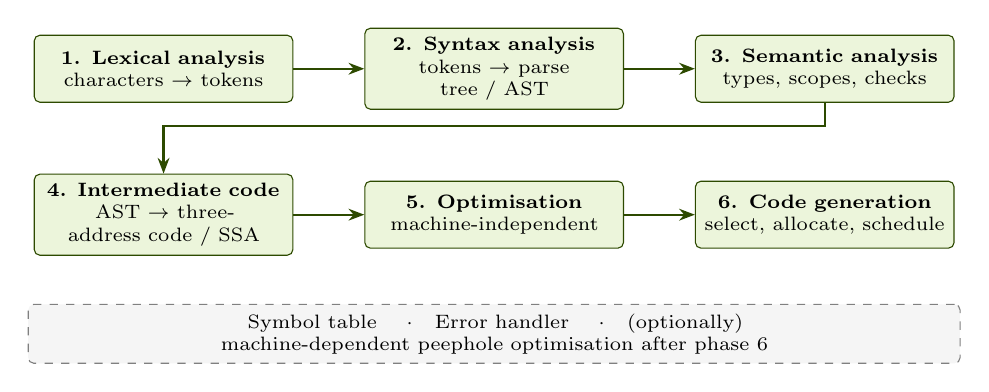
\begin{tikzpicture}[node distance=4mm and 9mm,every node/.style={font=\scriptsize},
 ph/.style={draw=nvdark,fill=nvgreen!14,rounded corners=2pt,minimum height=8.5mm,text width=3.05cm,align=center},
 data/.style={font=\tiny\itshape,text=black!70},
 arr/.style={-{Stealth[length=2mm]},thick,nvdark}]
\node[ph] (lex) {\textbf{1. Lexical analysis}\\ characters $\to$ tokens};
\node[ph,right=of lex] (syn) {\textbf{2. Syntax analysis}\\ tokens $\to$ parse tree / AST};
\node[ph,right=of syn] (sem) {\textbf{3. Semantic analysis}\\ types, scopes, checks};
\node[ph,below=9mm of lex] (ir) {\textbf{4. Intermediate code}\\ AST $\to$ three-address code / SSA};
\node[ph,right=of ir] (opt) {\textbf{5. Optimisation}\\ machine-independent};
\node[ph,right=of opt] (cg) {\textbf{6. Code generation}\\ select, allocate, schedule};
\draw[arr] (lex)--(syn); \draw[arr] (syn)--(sem);
\draw[arr] (sem.south) -- ++(0,-3mm) -| ([xshift=0mm]ir.north);
\draw[arr] (ir)--(opt); \draw[arr] (opt)--(cg);
\node[draw=black!50,dashed,rounded corners=2pt,fill=black!4,minimum height=7mm,text width=11.6cm,align=center,below=7mm of opt] (st)
 {Symbol table \quad$\cdot$\quad Error handler \quad$\cdot$\quad (optionally) machine-dependent peephole optimisation after phase 6};
\end{tikzpicture}
\end{center}
\begin{center}\small
\begin{tabularx}{\textwidth}{@{}L{3.2cm}L{4.1cm}Y@{}}
\toprule
\textbf{Phase} & \textbf{Output} & \textbf{Example for \texttt{a = b + 60}}\\
\midrule
Lexical & token stream & \texttt{id(a) = id(b) + num(60)}\\
Syntax & parse tree / AST & \texttt{=(a, +(b, 60))}\\
Semantic & annotated AST & \texttt{60} converted to float if \texttt{b} is float (inserted cast)\\
Intermediate code & TAC & \texttt{t1 = b + 60.0; a = t1}\\
Optimisation & better IR & constant folding, CSE, loop opts\\
Code generation & target code & \texttt{movss xmm0,[b]; addss xmm0,[c60]; movss [a],xmm0}\\
\bottomrule
\end{tabularx}
\end{center}
\textbf{Analysis vs.\ synthesis:} phases 1--3 \emph{analyse} the source (front end); 4--6 \emph{synthesise} the target. \textbf{Phase vs.\ pass:} a pass is one read of the program/IR; several phases may be grouped into one pass (a one-pass compiler is possible for simple languages; optimisers are many passes).

\begin{tipbox}[Frequently asked: ``Which phase detects \ldots?'']
Illegal character or malformed number: \textbf{lexical}. Missing semicolon, unbalanced parenthesis: \textbf{syntax}. Undeclared variable, type mismatch, wrong argument count, \texttt{break} outside a loop: \textbf{semantic}. Unreachable code, division by a constant zero: usually \textbf{semantic/optimisation} warnings. Out-of-bounds index and null dereference: \textbf{run time} (compilers cannot decide them in general).
\end{tipbox}

\section{The real C toolchain, stage by stage \prio{3}}
Everything below is real output for this four-line program.
\begin{lstlisting}[language={C}]
#include <stdio.h>
#define SQUARE(x) ((x) * (x))
int square_plus_one(int n) { return SQUARE(n) + 1; }
int main(void) { printf("%d\n", square_plus_one(7)); return 0; }
\end{lstlisting}
\textbf{1. Preprocessing} (\texttt{gcc -E}): includes and macros expanded; the compiler proper never sees the macro.
\begin{lstlisting}[style=shcmd]
$ gcc -E hello.c | tail -3
\end{lstlisting}
\begin{lstlisting}[style=out]
# 3 "hello.c"
int square_plus_one(int n) { return ((n) * (n)) + 1; }
int main(void) { printf("%d\n", square_plus_one(7)); return 0; }
\end{lstlisting}
\textbf{2. Compilation to assembly} (\texttt{gcc -S}): front end + optimiser + back end. At \texttt{-O0} every variable lives in memory (stack); that is why \texttt{-O0} code is slow but debuggable.
\begin{lstlisting}[style=shcmd]
$ gcc -S -O0 -masm=intel hello.c  # function square_plus_one
\end{lstlisting}
\begin{lstlisting}[style=out]
square_plus_one:
    push    rbp
    mov    rbp, rsp
    mov    DWORD PTR -4[rbp], edi
    mov    eax, DWORD PTR -4[rbp]
    imul    eax, eax
    add    eax, 1
    pop    rbp
    ret
\end{lstlisting}
\textbf{3. Assembly to an object file} (\texttt{gcc -c}), then \textbf{4. linking}: the object contains machine code and \emph{unresolved symbols}; the linker binds \texttt{printf} to the C library.
\begin{lstlisting}[style=shcmd]
$ gcc -c hello.c && nm hello.o && gcc hello.o -o hello && ./hello
\end{lstlisting}
\begin{lstlisting}[style=out]
0000000000000016 T main
                 U printf
0000000000000000 T square_plus_one
50
\end{lstlisting}
\texttt{T} = defined in the text section, \texttt{U} = undefined here (provided by another object/library). The five steps (preprocess, compile, assemble, link, load) are what ``\texttt{gcc hello.c}'' hides.

\section{Lexical analysis \prio{3}}
\begin{defbox}[Token, lexeme, pattern]
A \textbf{token} is a (name, attribute) pair handed to the parser (\texttt{id}, \texttt{num}, \texttt{if}, \texttt{+}). A \textbf{lexeme} is the actual character sequence (\texttt{count}, \texttt{60}). A \textbf{pattern} is the rule (a regular expression) describing a token's lexemes. The scanner skips whitespace and comments and enters identifiers into the symbol table.
\end{defbox}
\begin{mustbox}[Scanner rules examiners test]
\begin{itemize}[nosep]
\item \textbf{Longest match (maximal munch):} take the longest prefix that matches any pattern. So \texttt{x+++y} scans as \texttt{x ++ + y}, and \texttt{ifx} is one identifier, not \texttt{if} then \texttt{x}.
\item \textbf{Priority:} if two patterns match the same longest lexeme (\texttt{if} matches keyword and identifier), the rule listed first wins: put keywords before identifiers.
\item Regular expressions describe tokens because finite automata run in a single left-to-right pass with $O(1)$ work per character. Lexical errors: a character that starts no token; unterminated string/comment; malformed number.
\item Tools: \textbf{Lex/Flex} generate a DFA-driven scanner from a rule file; hand-written scanners use \texttt{switch} on the first character. Input is read through a two-buffer scheme with sentinels so end-of-buffer checks cost one comparison.
\end{itemize}
\end{mustbox}
\needspace{5\baselineskip}
\begin{lstlisting}[language={Python},title={A maximal-munch tokenizer, and the token-counting MCQ}]
import re
TOKEN = re.compile(r'''
    (?P<ws>\s+)
  | (?P<str>"(?:\\.|[^"\\])*")
  | (?P<num>\d+(?:\.\d+)?)
  | (?P<kw>(?:if|else|while|return|int)\b)       # BEFORE id, so keywords win ties
  | (?P<id>[A-Za-z_]\w*)
  | (?P<op>\+\+|--|<=|>=|==|!=|&&|\|\||->|[-+*/%<>=!&|^~?:;,.(){}\[\]])   # multi-char operators first
''', re.X)

def tokens(src):
    pos = 0
    while pos < len(src):
        m = TOKEN.match(src, pos)
        if not m: raise SyntaxError(f"lexical error at {pos}: {src[pos]!r}")
        pos = m.end()
        if m.lastgroup != "ws": yield (m.lastgroup, m.group())

for src in ['printf("%d", &i);', 'x = y+++z;', 'if (a<=b) return 1;', 'ifx = 3']:
    toks = list(tokens(src))
    print(len(toks), [t for _, t in toks])
\end{lstlisting}
\needspace{5\baselineskip}
\begin{lstlisting}[style=out,title={Answer: captured output}]
8 ['printf', '(', '"%d"', ',', '&', 'i', ')', ';']
7 ['x', '=', 'y', '++', '+', 'z', ';']
9 ['if', '(', 'a', '<=', 'b', ')', 'return', '1', ';']
3 ['ifx', '=', '3']
\end{lstlisting}
\textbf{Why:} \texttt{printf("\%d", \&i);} has 8 tokens (\texttt{printf ( "\%d" , \& i ) ;}); \texttt{x = y+++z;} has 7 because \texttt{+++} is munched as \texttt{++} then \texttt{+}; \texttt{ifx} is an identifier.

\section{Regular expressions and finite automata \prio{3}}
\begin{center}\small
\begin{tabularx}{\textwidth}{@{}L{4.6cm}Y@{}}
\toprule
\textbf{Regex operator (precedence high $\to$ low)} & \textbf{Meaning}\\
\midrule
\texttt{*} \;(Kleene star), \texttt{+}, \texttt{?} & zero or more, one or more, zero or one\\
concatenation \texttt{ab} & $a$ followed by $b$\\
union \texttt{a|b} & either\\
\bottomrule
\end{tabularx}
\end{center}
\begin{mustbox}[The equivalence cycle (and the sizes that blow up)]
Regex $\to$ \textbf{NFA} (Thompson's construction: at most $2|r|$ states, linear) $\to$ \textbf{DFA} (subset construction: worst case $2^n$ states) $\to$ \textbf{minimal DFA} (Hopcroft, $O(n\log n)$; unique up to renaming by Myhill--Nerode). A DFA has exactly one transition per symbol per state; an NFA may have none, several, or $\varepsilon$-moves. They recognise the \emph{same} class: the regular languages.
\textbf{Subset construction:} DFA state = set of NFA states; start = $\varepsilon$-closure of the NFA start; $\delta(S,a)=\varepsilon\text{-closure}(\text{move}(S,a))$; accepting if the set contains an NFA accepting state.
\end{mustbox}
\begin{exbox}[Worked example: $(a|b)^*abb$ --- the textbook NFA (11 states) $\to$ DFA $\to$ minimal DFA]
The script builds the Thompson-style NFA from the Dragon Book (states 0--10, accepting state 10), runs the subset construction, then minimises by partition refinement.
\end{exbox}
\needspace{5\baselineskip}
\begin{lstlisting}[language={Python},title={Subset construction and DFA minimisation for (a|b)*abb}]
eps = {0: [1, 7], 1: [2, 4], 3: [6], 5: [6], 6: [1, 7]}                       # epsilon moves
sym = {(2, 'a'): 3, (4, 'b'): 5, (7, 'a'): 8, (8, 'b'): 9, (9, 'b'): 10}      # symbol moves
start, accepting = 0, {10}

def closure(S):
    stack, out = list(S), set(S)
    while stack:
        for t in eps.get(stack.pop(), []):
            if t not in out: out.add(t); stack.append(t)
    return frozenset(out)
def move(S, a): return {sym[(s, a)] for s in S if (s, a) in sym}

A = closure({start}); names = {A: 'A'}; order = [A]; delta = {}
for S in order:                                  # 'order' grows while we iterate: BFS over DFA states
    for a in 'ab':
        T = closure(move(S, a))
        if T not in names: names[T] = chr(65 + len(names)); order.append(T)
        delta[(names[S], a)] = names[T]
for S in order:
    print(names[S], sorted(S), "accepting" if S & accepting else "")
print("DFA states:", len(order))
print({k: v for k, v in sorted(delta.items())})

# minimise: start with {accepting} / {non-accepting}, split until every block behaves uniformly
acc = {names[S] for S in order if S & accepting}
parts = [acc, set(names.values()) - acc]
changed = True
while changed:
    changed = False
    for P in list(parts):
        for a in 'ab':
            groups = {}
            for s in P:
                tgt = next(i for i, Q in enumerate(parts) if delta[(s, a)] in Q)
                groups.setdefault(tgt, set()).add(s)
            if len(groups) > 1:
                parts.remove(P); parts.extend(groups.values()); changed = True; break
        if changed: break
print("minimal DFA blocks:", sorted(sorted(P) for P in parts), "->", len(parts), "states")
\end{lstlisting}
\needspace{5\baselineskip}
\begin{lstlisting}[style=out,title={Captured output}]
A [0, 1, 2, 4, 7] 
B [1, 2, 3, 4, 6, 7, 8] 
C [1, 2, 4, 5, 6, 7] 
D [1, 2, 4, 5, 6, 7, 9] 
E [1, 2, 4, 5, 6, 7, 10] accepting
DFA states: 5
{('A', 'a'): 'B', ('A', 'b'): 'C', ('B', 'a'): 'B', ('B', 'b'): 'D', ('C', 'a'): 'B', ('C', 'b'): 'C', ('D', 'a'): 'B', ('D', 'b'): 'E', ('E', 'a'): 'B', ('E', 'b'): 'C'}
minimal DFA blocks: [['A', 'C'], ['B'], ['D'], ['E']] -> 4 states
\end{lstlisting}
\begin{center}
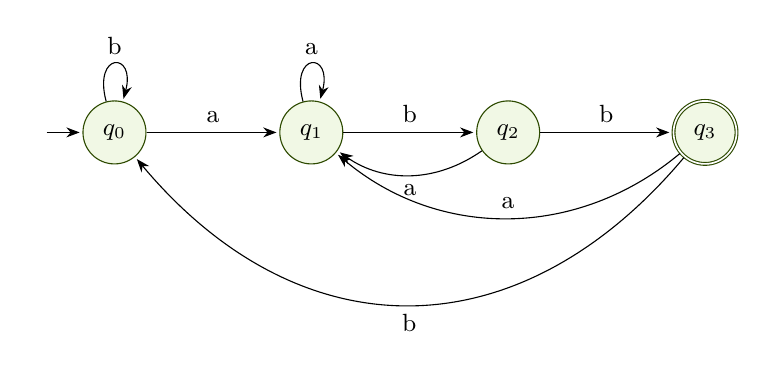
\begin{tikzpicture}[>=Stealth,shorten >=1pt,node distance=2.5cm,auto,font=\small,initial text=,
 every state/.style={draw=nvdark,fill=nvgreen!10,minimum size=8mm,inner sep=1pt}]
\node[state,initial] (q0) {$q_0$};
\node[state,right of=q0] (q1) {$q_1$};
\node[state,right of=q1] (q2) {$q_2$};
\node[state,accepting,right of=q2] (q3) {$q_3$};
\path[->] (q0) edge node {a} (q1)
 (q0) edge[loop above] node {b} ()
 (q1) edge node {b} (q2)
 (q1) edge[loop above] node {a} ()
 (q2) edge node {b} (q3)
 (q2) edge[bend left=35] node {a} (q1)
 (q3) edge[bend left=40] node[above] {a} (q1)
 (q3) edge[bend left=50,looseness=1.2] node[below] {b} (q0);
\end{tikzpicture}
\end{center}
\textbf{Reading the result:} the subset construction produces 5 DFA states $A$--$E$; states $A$ and $C$ behave identically (same transitions into the same blocks, both non-accepting), so the minimal DFA has 4 states: $q_0=\{A,C\}$, $q_1=B$, $q_2=D$, $q_3=E$. The state records ``how much of \texttt{abb} has been matched as a suffix''.

\subsection{Counting minimal DFA states (the standard MCQ family)}
\begin{center}\small
\begin{tabularx}{\textwidth}{@{}L{6.8cm}C{2.4cm}Y@{}}
\toprule
\textbf{Language over $\{a,b\}$} & \textbf{Minimal DFA states} & \textbf{Why}\\
\midrule
all strings ending in \texttt{ab} & 3 & remember the longest matching suffix: $\varepsilon$, \texttt{a}, \texttt{ab}\\
all strings ending in \texttt{abb} & 4 & as above, one more\\
strings with an even number of $a$'s & 2 & parity\\
strings whose length is a multiple of 3 & 3 & residue mod 3\\
the $k$-th symbol from the end is \texttt{a} & $2^k$ & a DFA must remember the last $k$ symbols (NFA needs $k+1$): the classic NFA$\to$DFA blow-up\\
strings containing \texttt{aa} & 3 & seen nothing / last was a / found\\
\bottomrule
\end{tabularx}
\end{center}
\begin{trapbox}[Regular vs.\ not]
A finite automaton has \emph{finite} memory. $\{a^nb^n\}$, balanced parentheses, $\{ww^R\}$, and ``number of $a$'s equals number of $b$'s'' are \textbf{not regular} (pumping lemma). Lexers therefore cannot match nested constructs: that is the parser's job (Chapter~\ref{ch:parsing}).
\end{trapbox}

\section{Practice \prio{3}}
\begin{qn}How many tokens are in \texttt{for (i = 0; i < n; i++) sum += a[i];}?\end{qn}
\begin{ans}\textbf{20} tokens: \texttt{for}, \texttt{(}, \texttt{i}, \texttt{=}, \texttt{0}, \texttt{;}, \texttt{i}, \texttt{<}, \texttt{n}, \texttt{;}, \texttt{i}, \texttt{++}, \texttt{)}, \texttt{sum}, \texttt{+=}, \texttt{a}, \texttt{[}, \texttt{i}, \texttt{]}, \texttt{;}. (\texttt{++} and \texttt{+=} are single tokens by maximal munch.)\end{ans}
\begin{qn}Which phase reports ``\texttt{error: 'x' undeclared}''? Which reports ``\texttt{expected ';' before 'return'}''?\end{qn}
\begin{ans}Undeclared identifier: \textbf{semantic analysis} (uses the symbol table). Missing semicolon: \textbf{syntax analysis}.\end{ans}
\begin{qn}A minimal DFA for strings over $\{0,1\}$ that are binary numbers divisible by 3 has how many states?\end{qn}
\begin{ans}\textbf{3}: track the remainder mod 3. Reading bit $b$ maps remainder $r$ to $(2r+b) \bmod 3$; the accepting state is remainder 0.\end{ans}
\begin{qn}True or false: every NFA with $n$ states has an equivalent DFA with at most $2^n$ states, and some need exactly that many.\end{qn}
\begin{ans}True: subset construction gives the upper bound, and the ``$n$-th symbol from the end'' languages show it is tight.\end{ans}
\begin{qn}Why must a lexer put keyword rules before the identifier rule?\end{qn}
\begin{ans}Both match \texttt{while} with the same length; the tie is broken by rule order. (An alternative is to match every identifier and look it up in a keyword table.)\end{ans}


% ===== 09-parsing.tex.in =====
\chapter{Syntax Analysis: Grammars and Parsing}
\label{ch:parsing}

\begin{chapbox}
\textbf{Priority \prio{3}. Time: 90 min.} Parsing is the most computational part of compiler theory and the standard source of numerical MCQs (FIRST/FOLLOW sets, LL(1) check, number of LR(0) states, conflict type, class of a grammar).
Every table and trace in this chapter was \emph{generated by a script} (Appendix~\ref{app:toolkit}) so the numbers are right.
\end{chapbox}



\section{Context-free grammars \prio{3}}
\begin{defbox}[Vocabulary]
A CFG is $G=(N,T,P,S)$: non-terminals, terminals, productions $A\to\alpha$, start symbol. A \textbf{derivation} $\Rightarrow$ rewrites a non-terminal; it is \textbf{leftmost} (always expand the leftmost non-terminal; top-down parsers find this) or \textbf{rightmost} (bottom-up parsers find it \emph{in reverse}). A \textbf{sentential form} is any string derivable from $S$; a \textbf{sentence} has only terminals. A \textbf{parse tree} shows the derivation structure; the \textbf{AST} is the parse tree with syntactic noise (parentheses, chain rules) removed.
\end{defbox}
\subsection{Ambiguity, precedence and associativity}
A grammar is \textbf{ambiguous} if some sentence has two parse trees (equivalently two leftmost derivations). $E\to E+E\mid E*E\mid\texttt{id}$ is ambiguous: \texttt{id+id*id} can group as \texttt{(id+id)*id} or \texttt{id+(id*id)}. The fix encodes precedence by \emph{layering} and associativity by the \emph{direction of recursion}:
\begin{center}
\begin{tabular}{@{}ll@{}}
\toprule
\textbf{Ambiguous} & \textbf{Unambiguous (left-assoc.\ $+$, $*$; $*$ binds tighter)}\\
\midrule
$E\to E+E\mid E*E\mid(E)\mid \texttt{id}$ & $E\to E+T\mid T;\quad T\to T*F\mid F;\quad F\to(E)\mid\texttt{id}$\\
\bottomrule
\end{tabular}
\end{center}
\begin{mustbox}[Rules of thumb]
\begin{itemize}[nosep]
\item \textbf{Left recursion} ($E\to E+T$) makes an operator \emph{left}-associative; \textbf{right recursion} ($E\to T^{\wedge}E$) makes it \emph{right}-associative (exponentiation, assignment, \texttt{?:}).
\item Operators lower in the grammar (deeper non-terminals) bind \emph{tighter}.
\item Ambiguity is undecidable in general; there is no algorithm that always removes it. The \textbf{dangling else} (\texttt{if E then S | if E then S else S}) is the classic: the usual fix attaches \texttt{else} to the nearest \texttt{if} via ``matched/unmatched'' statements, or the parser generator resolves the shift/reduce conflict in favour of \emph{shift}.
\end{itemize}
\end{mustbox}

\subsection{Grammar transformations a top-down parser needs}
\begin{center}\small
\begin{tabularx}{\textwidth}{@{}L{3.6cm}L{5.6cm}Y@{}}
\toprule
\textbf{Problem} & \textbf{Transformation} & \textbf{Example}\\
\midrule
Immediate left recursion & $A\to A\alpha\mid\beta\ \Longrightarrow\ A\to\beta A',\ A'\to\alpha A'\mid\varepsilon$ & $E\to E+T\mid T$ becomes $E\to TE',\ E'\to+TE'\mid\varepsilon$\\
Indirect left recursion & order the non-terminals $A_1..A_n$; substitute earlier ones into later ones, then remove immediate recursion & $S\to Aa,\ A\to Sb\mid c$: substitute $S$ in $A$\\
Common prefix & left factoring: $A\to\alpha\beta_1\mid\alpha\beta_2\ \Longrightarrow\ A\to\alpha A',\ A'\to\beta_1\mid\beta_2$ & $S\to iEtS\mid iEtSeS$ becomes $S\to iEtSS'$, $S'\to eS\mid\varepsilon$\\
\bottomrule
\end{tabularx}
\end{center}
These transformations preserve the language (not the tree shape; semantic actions need care). Left recursion is fine for \emph{bottom-up} parsers: it uses less stack there.

\section{Top-down parsing and LL(1) \prio{3}}
\subsection{Recursive descent: one function per non-terminal}
\begin{mustbox}
Turn the left-recursive rule into a loop (EBNF): $E\to T\,\{(+|-)\,T\}$, $T\to F\,\{(*|/)\,F\}$, $F\to\textit{num}\mid(E)\mid -F$. Each function consumes tokens and returns a value (or an AST node). \textbf{Left-associativity falls out of the loop.} A \emph{right}-recursive rule for $-$ would compute $10-(4-3)$ instead of $(10-4)-3$.
\end{mustbox}
\needspace{5\baselineskip}
\begin{lstlisting}[language={Python},title={Recursive-descent evaluator (and the right-recursion associativity bug)}]
import re

def tokenize(s): return re.findall(r"\d+|[-+*/()]", s)

class Parser:
    def __init__(self, text): self.t, self.i = tokenize(text), 0
    def peek(self): return self.t[self.i] if self.i < len(self.t) else None
    def eat(self, expect=None):
        tok = self.peek()
        if tok is None or (expect and tok != expect): raise SyntaxError(f"expected {expect!r}, got {tok!r}")
        self.i += 1; return tok
    def expr(self):                                   # E -> T { (+|-) T }      (left-associative via the loop)
        v = self.term()
        while self.peek() in ("+", "-"):
            op = self.eat(); r = self.term()
            v = v + r if op == "+" else v - r
        return v
    def term(self):                                   # T -> F { (*|/) F }
        v = self.factor()
        while self.peek() in ("*", "/"):
            op = self.eat(); r = self.factor()
            v = v * r if op == "*" else v / r
        return v
    def factor(self):                                 # F -> num | ( E ) | - F
        tok = self.peek()
        if tok == "(": self.eat("("); v = self.expr(); self.eat(")"); return v
        if tok == "-": self.eat("-"); return -self.factor()
        return int(self.eat())
    def expr_right_recursive(self):                   # WRONG on purpose: E -> T [ - E ]  (right-associative minus)
        v = self.term()
        if self.peek() == "-": self.eat(); return v - self.expr_right_recursive()
        return v

for src in ["2+3*(4-1)", "10-4-3", "2*3+4*5", "-(2+3)*2", "100/5/2"]:
    print(f"{src:12} = {Parser(src).expr()}")
print("10-4-3 with right recursion =", Parser("10-4-3").expr_right_recursive(), "(wrong: should be 3)")
\end{lstlisting}
\needspace{5\baselineskip}
\begin{lstlisting}[style=out,title={Answer: captured output}]
2+3*(4-1)    = 11
10-4-3       = 3
2*3+4*5      = 26
-(2+3)*2     = -10
100/5/2      = 10.0
10-4-3 with right recursion = 9 (wrong: should be 3)
\end{lstlisting}

\subsection{FIRST and FOLLOW}
\begin{mustbox}[Definitions and rules]
\textbf{FIRST($\alpha$)}: set of terminals that can begin a string derived from $\alpha$ (plus $\varepsilon$ if $\alpha\Rightarrow^*\varepsilon$). \textbf{FOLLOW($A$)}: set of terminals that can appear immediately to the right of $A$ in some sentential form ($\$\in$ FOLLOW(start)); \textbf{FOLLOW never contains $\varepsilon$.}
\begin{enumerate}[nosep]
\item FIRST(terminal) = \{terminal\}. For $X\to Y_1Y_2\ldots Y_k$: add FIRST($Y_1$)$\setminus\{\varepsilon\}$; if $\varepsilon\in$ FIRST($Y_1$) add FIRST($Y_2$)$\setminus\{\varepsilon\}$, and so on; if all $Y_i$ can vanish add $\varepsilon$.
\item FOLLOW: for $A\to\alpha B\beta$ add FIRST($\beta$)$\setminus\{\varepsilon\}$ to FOLLOW($B$); if $\varepsilon\in$ FIRST($\beta$) (or $\beta$ is empty) add FOLLOW($A$) to FOLLOW($B$). Repeat until nothing changes.
\end{enumerate}
\end{mustbox}
\begin{mustbox}[LL(1) condition]
A grammar is \textbf{LL(1)} iff for every non-terminal $A$ with alternatives $\alpha_1\mid\alpha_2\mid\cdots$: (i) FIRST($\alpha_i$) $\cap$ FIRST($\alpha_j$) $=\emptyset$ for $i\ne j$; (ii) at most one alternative derives $\varepsilon$; (iii) if $\alpha_i\Rightarrow^*\varepsilon$ then FIRST($\alpha_j$) $\cap$ FOLLOW($A$) $=\emptyset$ for $j\ne i$. Consequences: \textbf{no LL(1) grammar is left-recursive or ambiguous}, and the parse table has at most one entry per cell. The first L: scan Left-to-right; the second L: Leftmost derivation; (1): one token of lookahead.
\end{mustbox}
The expression grammar made LL(1) by removing left recursion:
\needspace{5\baselineskip}
\begin{lstlisting}[language={Python},title={FIRST, FOLLOW and the LL(1) table for the transformed expression grammar}]
from lrtool import *
LL1 = """E -> T E'
E' -> + T E' | eps
T -> F T'
T' -> * F T' | eps
F -> ( E ) | id"""
g = parse_grammar(LL1)
show_grammar(g)
first, follow, _ = first_follow(g, "E")
for A in g: print("  FIRST(%s) = %-14s FOLLOW(%s) = %s" % (A, sorted(first[A]), A, sorted(follow[A])))
print_ll1_table(g, "E")
\end{lstlisting}
\needspace{5\baselineskip}
\begin{lstlisting}[style=out,title={Captured output}]
  (1) E -> T E'
  (2) E' -> + T E'
  (3) E' -> eps
  (4) T -> F T'
  (5) T' -> * F T'
  (6) T' -> eps
  (7) F -> ( E )
  (8) F -> id
  FIRST(E) = ['(', 'id']    FOLLOW(E) = ['$', ')']
  FIRST(E') = ['+', 'eps']   FOLLOW(E') = ['$', ')']
  FIRST(T) = ['(', 'id']    FOLLOW(T) = ['$', ')', '+']
  FIRST(T') = ['*', 'eps']   FOLLOW(T') = ['$', ')', '+']
  FIRST(F) = ['(', 'id']    FOLLOW(F) = ['$', ')', '*', '+']
  M[E,(] = E -> T E'
  M[E,id] = E -> T E'
  M[E',$] = E' -> eps
  M[E',)] = E' -> eps
  M[E',+] = E' -> + T E'
  M[F,(] = F -> ( E )
  M[F,id] = F -> id
  M[T,(] = T -> F T'
  M[T,id] = T -> F T'
  M[T',$] = T' -> eps
  M[T',)] = T' -> eps
  M[T',*] = T' -> * F T'
  M[T',+] = T' -> eps
  conflicts: none  => the grammar is LL(1)
\end{lstlisting}
\textbf{How to read it:} an entry \texttt{M[A,a] = A -> \$\textbackslash{}alpha\$} means ``when $A$ is on top of the stack and the next token is $a$, expand with $\alpha$''. The $\varepsilon$-productions $E'\to\varepsilon$ and $T'\to\varepsilon$ appear exactly under the tokens in FOLLOW($E'$) and FOLLOW($T'$): that is why FOLLOW sets matter. No cell has two entries, so the grammar is LL(1).
\subsection{The predictive parser in action}
\needspace{5\baselineskip}
\begin{lstlisting}[language={Python},title={Table-driven LL(1) parse of  id + id * id}]
from lrtool import *
g = parse_grammar("""E -> T E'
E' -> + T E' | eps
T -> F T'
T' -> * F T' | eps
F -> ( E ) | id""")
ll1_parse(g, "E", ["id", "+", "id", "*", "id"])
\end{lstlisting}
\needspace{5\baselineskip}
\begin{lstlisting}[style=out,title={Captured output}]
  STACK (top at right)       INPUT              ACTION
  $ E                        id + id * id $     E -> T E'
  $ E' T                     id + id * id $     T -> F T'
  $ E' T' F                  id + id * id $     F -> id
  $ E' T' id                 id + id * id $     match id
  $ E' T'                    + id * id $        T' -> eps
  $ E'                       + id * id $        E' -> + T E'
  $ E' T +                   + id * id $        match +
  $ E' T                     id * id $          T -> F T'
  $ E' T' F                  id * id $          F -> id
  $ E' T' id                 id * id $          match id
  $ E' T'                    * id $             T' -> * F T'
  $ E' T' F *                * id $             match *
  $ E' T' F                  id $               F -> id
  $ E' T' id                 id $               match id
  $ E' T'                    $                  T' -> eps
  $ E'                       $                  E' -> eps
  $                          $                  accept
\end{lstlisting}
\begin{trapbox}[LL(1) checks examiners love (all verified by the script)]
\begin{itemize}[nosep]
\item $E\to E+T\mid T$: not LL(1) --- \textbf{left recursion}. $S\to iEtS\mid iEtSeS\mid a$ (the dangling else): not LL(1) --- common prefix, and ambiguous.
\item $S\to AB,\ A\to a\mid\varepsilon,\ B\to b\mid\varepsilon$ \emph{is} LL(1): FIRST(S)=\{a,b,$\varepsilon$\}, FOLLOW(A)=\{b,\$\}, FOLLOW(B)=\{\$\}. And $S\to(S)S\mid\varepsilon$ (balanced parentheses) is LL(1).
\item Palindromes $S\to aSa\mid bSb\mid a\mid b\mid\varepsilon$ cannot be parsed deterministically by \emph{any} LL or LR parser: the middle of the string cannot be recognised with bounded lookahead (it is not a deterministic CFL).
\end{itemize}
\end{trapbox}
\textbf{Error recovery:} \emph{panic mode} skips tokens until one in a \emph{synchronising set} (usually FOLLOW of the current non-terminal plus statement-start keywords) is found; \emph{phrase-level} recovery inserts or deletes tokens locally; \emph{error productions} add known common mistakes to the grammar; \emph{global correction} (minimum edits) is too expensive in practice.

\section{Bottom-up parsing: LR family \prio{3}}
\begin{mustbox}
A \textbf{shift-reduce} parser keeps a stack of grammar symbols. \textbf{Shift}: push the next token. \textbf{Reduce}: when the top of the stack matches the right side of a production (a \textbf{handle}), pop it and push the left side. \textbf{Accept} when the stack is the start symbol and input is exhausted. It traces a \emph{rightmost derivation in reverse}. An LR parser decides by consulting an automaton whose states are sets of \textbf{LR items} $A\to\alpha\cdot\beta$ (``I have seen $\alpha$, expect $\beta$'').
\end{mustbox}
\begin{center}\small
\begin{tabularx}{\textwidth}{@{}L{2.6cm}L{4.6cm}Y@{}}
\toprule
\textbf{Parser} & \textbf{Items / lookahead for a reduce} & \textbf{Power and size}\\
\midrule
LR(0) & items only; reduce in a state regardless of the next token & weakest; conflicts as soon as a state has a reduce plus anything else\\
\textbf{SLR(1)} & reduce $A\to\alpha$ on tokens in FOLLOW($A$) & simple, small tables (same states as LR(0))\\
\textbf{LALR(1)} & merge LR(1) states that have the \emph{same core}, keeping precise lookaheads & same number of states as SLR; \textbf{Yacc/Bison default}\\
\textbf{LR(1) (canonical)} & items carry one lookahead token $[A\to\alpha\cdot\beta,\ a]$ & most powerful; many more states\\
\bottomrule
\end{tabularx}
\end{center}
\begin{center}
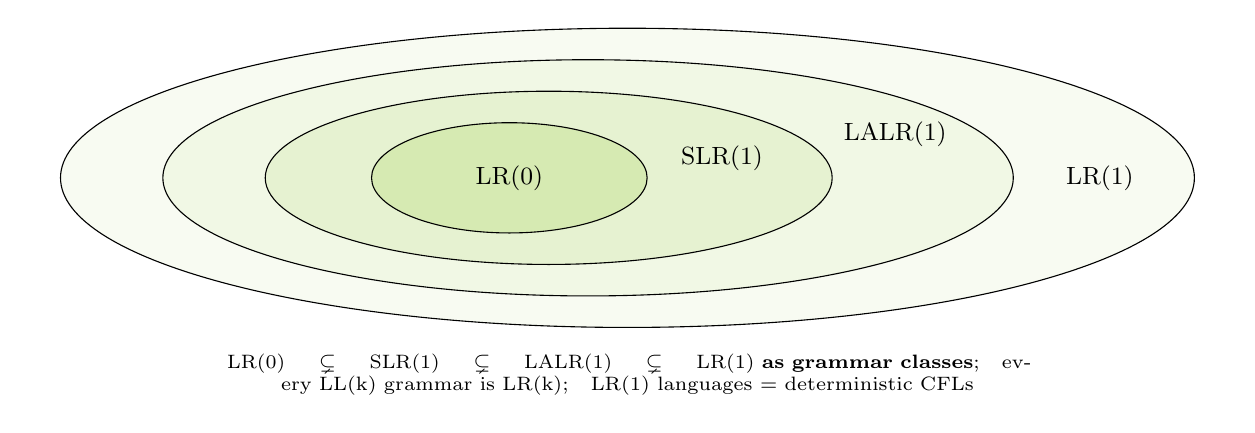
\begin{tikzpicture}[font=\small]
\draw[fill=nvgreen!5] (0,0) ellipse (7.2cm and 1.9cm);
\draw[fill=nvgreen!10] (-0.5,0) ellipse (5.4cm and 1.5cm);
\draw[fill=nvgreen!18] (-1.0,0) ellipse (3.6cm and 1.1cm);
\draw[fill=nvgreen!30] (-1.5,0) ellipse (1.75cm and 0.7cm);
\node at (-1.5,0) {LR(0)};
\node at (1.2,0.25) {SLR(1)};
\node at (3.4,0.55) {LALR(1)};
\node at (6.0,0) {LR(1)};
\node[font=\scriptsize,align=center,text width=15cm] at (0,-2.5) {$\mathrm{LR(0)}\subsetneq\mathrm{SLR(1)}\subsetneq\mathrm{LALR(1)}\subsetneq\mathrm{LR(1)}$ \textbf{as grammar classes};\quad every LL(k) grammar is LR(k);\quad LR(1) languages $=$ deterministic CFLs};
\end{tikzpicture}
\end{center}
\subsection{The SLR(1) construction, verified}
\textbf{Construction recipe:} (1) augment with $S'\to S$; (2) \emph{closure}$(I)$: while an item has the dot before a non-terminal $B$, add $B\to\cdot\gamma$ for all its productions; (3) \emph{goto}$(I,X)$: move the dot over $X$ in every item that allows it, then close; (4) build all states from $I_0$; (5) \textbf{shift} on terminal $a$ if goto exists; \textbf{reduce} $A\to\alpha$ on each $a\in$ FOLLOW($A$) when $A\to\alpha\cdot$ is in the state; \textbf{accept} on \$ for $S'\to S\cdot$; \textbf{goto} entries for non-terminals. If any cell receives two actions, the grammar is not SLR(1).
\needspace{5\baselineskip}
\begin{lstlisting}[language={Python},title={SLR(1) table for  E -> E+T | T ;  T -> T*F | F ;  F -> (E) | id}]
from lrtool import *
g = parse_grammar("""E -> E + T | T
T -> T * F | F
F -> ( E ) | id""")
show_grammar(g)
print_slr(g, "E")
\end{lstlisting}
\needspace{5\baselineskip}
\begin{lstlisting}[style=out,title={Captured output}]
  (1) E -> E + T
  (2) E -> T
  (3) T -> T * F
  (4) T -> F
  (5) F -> ( E )
  (6) F -> id
  state | +    *    (    )    id   $    | E   T   F  
      0 |           s3        s4        | 1   2   5  
      1 | s6                       acc  |            
      2 | r2   s7        r2        r2   |            
      3 |           s3        s4        | 8   2   5  
      4 | r6   r6        r6        r6   |            
      5 | r4   r4        r4        r4   |            
      6 |           s3        s4        |     9   5  
      7 |           s3        s4        |         10 
      8 | s6             s11            |            
      9 | r1   s7        r1        r1   |            
     10 | r3   r3        r3        r3   |            
     11 | r5   r5        r5        r5   |            
  conflicts: 0
\end{lstlisting}
\textbf{Reading the table:} \texttt{s4} = ``shift and go to state 4''; \texttt{r6} = ``reduce by production 6 ($F\to\textit{id}$)''; the right block is GOTO. There are \textbf{12 states} and no conflicts. State 4 contains the single complete item $F\to\textit{id}\cdot$ so it reduces on any token in FOLLOW($F$)$=\{+,*,),\$\}$. State 2 has both $E\to T\cdot$ (reduce on FOLLOW($E$)$=\{+,),\$\}$) and $T\to T\cdot{*}F$ (shift on \texttt{*}); the two token sets are disjoint, so there is no conflict: this is what the lookahead buys over LR(0).
\needspace{5\baselineskip}
\begin{lstlisting}[language={Python},title={LR parse of  id * id + id : each reduce is one step of a rightmost derivation (in reverse)}]
from lrtool import *
g = parse_grammar("""E -> E + T | T
T -> T * F | F
F -> ( E ) | id""")
lr_parse(g, "E", ["id", "*", "id", "+", "id"])
\end{lstlisting}
\needspace{5\baselineskip}
\begin{lstlisting}[style=out,title={Captured output}]
  STATES               SYMBOLS          INPUT            ACTION
  0                                     id * id + id $   shift 4
  0 4                  id               * id + id $      reduce 6: F -> id
  0 5                  F                * id + id $      reduce 4: T -> F
  0 2                  T                * id + id $      shift 7
  0 2 7                T *              id + id $        shift 4
  0 2 7 4              T * id           + id $           reduce 6: F -> id
  0 2 7 10             T * F            + id $           reduce 3: T -> T * F
  0 2                  T                + id $           reduce 2: E -> T
  0 1                  E                + id $           shift 6
  0 1 6                E +              id $             shift 4
  0 1 6 4              E + id           $                reduce 6: F -> id
  0 1 6 5              E + F            $                reduce 4: T -> F
  0 1 6 9              E + T            $                reduce 1: E -> E + T
  0 1                  E                $                accept
\end{lstlisting}
The parse performed \textbf{8 reductions} (6, 4, 6, 3, 2, 6, 4, 1), which is the number of productions in the rightmost derivation; \textbf{5 shifts} (one per token). Note that \texttt{id*id} was reduced to $T$ \emph{before} the \texttt{+} was shifted: that is precedence at work.

\subsection{Conflicts and the grammar classes, verified}
\begin{mustbox}[Conflicts]
\textbf{Shift/reduce:} a state wants to shift token $a$ and also reduce on $a$ (typical cause: ambiguity, e.g.\ dangling else, or too weak a lookahead). \textbf{Reduce/reduce:} two different complete items could be reduced on the same token (typical cause: two non-terminals deriving the same string). Parser generators: default $=$ prefer \emph{shift}; for reduce/reduce choose the \emph{earlier} production. \textbf{Ambiguous grammars are never LR(k)} for any $k$.
\end{mustbox}
\needspace{5\baselineskip}
\begin{lstlisting}[language={Python},title={Which class does each grammar belong to? (counts of states and conflicts)}]
from lrtool import *
G = {
 "expr":  ("E", "E -> E + T | T\nT -> T * F | F\nF -> ( E ) | id"),
 "LL1":   ("E", "E -> T E'\nE' -> + T E' | eps\nT -> F T'\nT' -> * F T' | eps\nF -> ( E ) | id"),
 "G2":    ("S", "S -> L = R | R\nL -> * R | id\nR -> L"),
 "G3":    ("S", "S -> a A d | b B d | a B e | b A e\nA -> c\nB -> c"),
 "dangle":("S", "S -> i E t S | i E t S e S | a\nE -> b"),
 "AB":    ("S", "S -> A B\nA -> a | eps\nB -> b | eps"),
 "paren": ("S", "S -> ( S ) S | eps"),
 "palin": ("S", "S -> a S a | b S b | a | b | eps"),
 "ambig": ("E", "E -> E + E | E * E | id"),
}
for name, (start, text) in G.items(): classify(name, text, start)
\end{lstlisting}
\needspace{5\baselineskip}
\begin{lstlisting}[style=out,title={Captured output}]
expr    LL(1)=no  | LR(0): 12 states | SLR conflicts  0 | LR(1): 22 st,  0 confl | LALR: 12 st,  0 confl
LL1     LL(1)=yes | LR(0): 16 states | SLR conflicts  0 | LR(1): 30 st,  0 confl | LALR: 16 st,  0 confl
G2      LL(1)=no  | LR(0): 10 states | SLR conflicts  1 | LR(1): 14 st,  0 confl | LALR: 10 st,  0 confl
G3      LL(1)=no  | LR(0): 13 states | SLR conflicts  2 | LR(1): 14 st,  0 confl | LALR: 13 st,  2 confl
dangle  LL(1)=no  | LR(0): 10 states | SLR conflicts  1 | LR(1): 17 st,  1 confl | LALR: 10 st,  1 confl
AB      LL(1)=yes | LR(0):  6 states | SLR conflicts  0 | LR(1):  6 st,  0 confl | LALR:  6 st,  0 confl
paren   LL(1)=yes | LR(0):  6 states | SLR conflicts  0 | LR(1): 10 st,  0 confl | LALR:  6 st,  0 confl
palin   LL(1)=no  | LR(0):  8 states | SLR conflicts  8 | LR(1): 20 st,  8 confl | LALR:  8 st,  4 confl
ambig   LL(1)=no  | LR(0):  7 states | SLR conflicts  4 | LR(1):  7 st,  4 confl | LALR:  7 st,  4 confl
\end{lstlisting}
\begin{center}\small
\begin{tabularx}{\textwidth}{@{}L{2.0cm}Y@{}}
\toprule
\textbf{Grammar} & \textbf{Lesson}\\
\midrule
\texttt{expr} & Left-recursive, so not LL(1), but SLR(1): \textbf{12 LR(0) states, 22 canonical LR(1) states, 12 LALR states}. LALR has exactly as many states as LR(0); canonical LR(1) splits states by lookahead.\\
\texttt{G2} & The pointer-assignment grammar $S\to L=R\mid R,\ L\to *R\mid \textit{id},\ R\to L$ is \textbf{not SLR(1)} (one shift/reduce conflict: FOLLOW($R$) contains \texttt{=}, though a reduce $R\to L$ before \texttt{=} is never valid) but \textbf{is LALR(1)} and LR(1). A famous exam example.\\
\texttt{G3} & $S\to aAd\mid bBd\mid aBe\mid bAe,\ A\to c,\ B\to c$ is \textbf{LR(1) but not LALR(1)}: after \texttt{ac} and \texttt{bc} the LR(1) states differ only in lookaheads, merging them creates a reduce/reduce conflict. (Not SLR(1) either.)\\
\texttt{dangle}, \texttt{ambig} & Ambiguous: conflicts in \emph{every} LR variant.\\
\texttt{palin} & Inherently non-deterministic context-free language: many conflicts everywhere.\\
\bottomrule
\end{tabularx}
\end{center}

\section{Parser generators and what real compilers do \prio{2}}
\begin{itemize}[nosep]
\item \textbf{Yacc/Bison:} LALR(1) generator. A rule file with semantic actions (\texttt{\$\$ = \$1 + \$3;}); precedence/associativity declarations (\texttt{\%left '+' '-'}, \texttt{\%left '*' '/'}, \texttt{\%right '\textasciicircum{}'}, \texttt{\%prec} for unary minus) resolve the shift/reduce conflicts of an ambiguous expression grammar \emph{without} the layered rewrite. Bison also offers GLR parsing for ambiguous grammars.
\item \textbf{ANTLR} generates LL(*)/ALL(*) recursive-descent parsers; \textbf{PEG/packrat} parsers use ordered choice.
\item \textbf{Hand-written recursive descent} is what production compilers use: Clang and GCC's C and C++ front ends are hand-written. Reasons: precise error messages and recovery, easy context-sensitive tricks (C++ needs the symbol table to know whether \texttt{a * b;} declares a pointer or multiplies), speed, and flexibility. \textbf{Pratt (precedence-climbing) parsing} handles expressions compactly (next chapter).
\item C and C++ are \textbf{not} context-free as written (typedef names, templates): parsing consults the symbol table (the ``lexer hack'').
\end{itemize}

\section{Formal-language facts that appear in MCQs \prio{2}}
\begin{center}\small
\begin{tabularx}{\textwidth}{@{}L{3.1cm}L{3.0cm}Y@{}}
\toprule
\textbf{Chomsky class} & \textbf{Automaton} & \textbf{Examples / key facts}\\
\midrule
Type 3 regular & DFA / NFA & lexical tokens; closed under union, concatenation, star, complement, intersection; pumping lemma shows $a^nb^n$ is not regular\\
Type 2 context-free & PDA (non-deterministic) & balanced parentheses, $a^nb^n$, palindromes; closed under union, concatenation, star; \textbf{not} closed under intersection or complement; \textbf{DPDA $\subsetneq$ NPDA}\\
Type 1 context-sensitive & linear bounded automaton & $a^nb^nc^n$ (not context-free)\\
Type 0 recursively enumerable & Turing machine & halting problem's yes-instances\\
\bottomrule
\end{tabularx}
\end{center}

\section{Practice \prio{3}}
\begin{qn}Compute FIRST and FOLLOW for $S\to AB,\ A\to a\mid\varepsilon,\ B\to b\mid\varepsilon$.\end{qn}
\begin{lstlisting}[language={Python}]
from lrtool import *
g = parse_grammar("S -> A B\nA -> a | eps\nB -> b | eps")
first, follow, _ = first_follow(g, "S")
for A in g: print("FIRST(%s) = %-12s FOLLOW(%s) = %s" % (A, sorted(first[A]), A, sorted(follow[A])))
\end{lstlisting}
\needspace{5\baselineskip}
\begin{lstlisting}[style=out,title={Answer: captured output}]
FIRST(S) = ['a', 'b', 'eps'] FOLLOW(S) = ['$']
FIRST(A) = ['a', 'eps'] FOLLOW(A) = ['$', 'b']
FIRST(B) = ['b', 'eps'] FOLLOW(B) = ['$']
\end{lstlisting}
\textbf{Why:} FIRST(S) includes \texttt{a}; since $A$ can vanish it also includes FIRST(B)=\{b\}; since both can vanish, $\varepsilon\in$ FIRST(S). FOLLOW(A) gets FIRST(B)$\setminus\{\varepsilon\}=\{b\}$ and, because $B$ vanishes, FOLLOW(S)=\{\$\}.
\begin{qn}How many reduce moves does an LR parser make for \texttt{id+id*id} with the expression grammar?\end{qn}
\begin{ans}One reduction per production in the rightmost derivation: $F\to\textit{id}$ three times, $T\to F$ twice, $T\to T*F$ once, $E\to T$ once, $E\to E+T$ once, total \textbf{8}. (Shifts: one per token, so 5.)\end{ans}
\begin{qn}True or false: (a) every LL(1) grammar is LR(1); (b) every LR(1) grammar is LL(1); (c) LALR(1) tables are smaller than canonical LR(1) tables; (d) an ambiguous grammar can be LR(1).\end{qn}
\begin{ans}(a) \textbf{True}. (b) False: the left-recursive expression grammar is LR(1) but not LL(1). (c) \textbf{True} (merging same-core states; 12 vs.\ 22 above). (d) False: LR(1) grammars are unambiguous.\end{ans}
\begin{qn}Which of these cannot be recognised by a regular expression/DFA? (i) strings over $\{a,b\}$ with equal numbers of $a$ and $b$; (ii) strings ending in \texttt{ab}; (iii) binary numbers divisible by 5.\end{qn}
\begin{ans}Only (i): counting needs unbounded memory. (ii) and (iii) are regular (3 and 5 states respectively).\end{ans}
\begin{qn}In an SLR(1) table, when can a state have both a shift on $a$ and a reduce on $a$ without being a conflict?\end{qn}
\begin{ans}Never: two actions in one cell is by definition a conflict. State 2 above has a shift on \texttt{*} and reduces on \texttt{+, ), \$}: different cells, so no conflict.\end{ans}
\begin{qn}Give the left-recursion-free equivalent of $A\to Ab\mid Ac\mid d$.\end{qn}
\begin{ans}$A\to dA'$, $A'\to bA'\mid cA'\mid\varepsilon$ (generates $d(b|c)^*$).\end{ans}


% ===== 10-semantic-ir.tex.in =====
\chapter{Semantic Analysis, Intermediate Code, SSA, Runtime}
\label{ch:sem}

\begin{chapbox}
\textbf{Priority \prio{3} for IR/SSA and runtime, \prio{2} for SDD/types. Time: 80 min.} Intermediate representations (three-address code, SSA) are the language of optimisers and of LLVM/PTX. Runtime topics (activation records, parameter passing, GC) are classic MCQ material.
The chapter ends with a \textbf{working mini compiler} (Appendix~\ref{app:tiny}) that is reused in the verification lab (Chapter~\ref{ch:lab}).
\end{chapbox}




\section{Syntax-directed definitions and translation \prio{2}}
\begin{mustbox}
An \textbf{SDD} attaches \emph{attributes} to grammar symbols and \emph{semantic rules} to productions. \textbf{Synthesised} attributes are computed from children (bottom-up); \textbf{inherited} attributes from parent and siblings (top-down). \textbf{S-attributed}: synthesised only (evaluable during an LR parse by reduce-time actions). \textbf{L-attributed}: inherited attributes may depend only on the parent and \emph{left} siblings (evaluable in one left-to-right depth-first pass, so suitable for LL parsers and recursive descent). A \textbf{translation scheme (SDT)} embeds the actions in the productions at the exact point they run.
\end{mustbox}
\begin{center}\small
\begin{tabularx}{\textwidth}{@{}L{3.6cm}L{4.4cm}Y@{}}
\toprule
\textbf{Production} & \textbf{Semantic rule} & \textbf{Kind}\\
\midrule
$E\to E_1+T$ & $E.val = E_1.val + T.val$ & synthesised\\
$T\to T_1*F$ & $T.val = T_1.val\times F.val$ & synthesised\\
$F\to \textit{digit}$ & $F.val = \textit{digit}.lexval$ & synthesised (S-attributed overall)\\
$D\to T\,L$ & $L.inh = T.type$ & \textbf{inherited} (declaration \texttt{int a, b, c;})\\
$L\to L_1,\ \textit{id}$ & $L_1.inh = L.inh;\ \mathrm{addtype}(\textit{id}.entry, L.inh)$ & inherited, L-attributed\\
\bottomrule
\end{tabularx}
\end{center}
\textbf{Typical uses:} evaluating constant expressions, building the AST, \emph{type checking}, generating intermediate code, filling the symbol table with declared types.

\section{Types, scopes and symbol tables \prio{2}}
\begin{itemize}[nosep]
\item \textbf{Static vs.\ dynamic typing:} types checked at compile time (C, C++, Rust) vs.\ at run time (Python). \textbf{Strong vs.\ weak:} whether implicit unsafe conversions are allowed (C is weakly typed: \texttt{int} to pointer casts).
\item \textbf{Type equivalence:} \emph{name} equivalence (two types are the same only if they have the same declared name; C structs) vs.\ \emph{structural} equivalence (same shape). \textbf{Coercion}: implicit conversion inserted by the compiler (\texttt{int} to \texttt{float} in \texttt{a + 1.5}); \textbf{cast}: explicit.
\item \textbf{Overloading} (several functions, one name, resolved by argument types) vs.\ \textbf{polymorphism}: parametric (templates/generics), subtype (virtual functions), ad hoc (overloading). \textbf{Type inference} (Hindley--Milner, \texttt{auto}) deduces types by unification: $\lambda x.\,x+1$ gets type $\mathit{int}\to\mathit{int}$.
\item \textbf{Symbol table:} maps names to attributes (type, scope, offset, storage class). Implementation: a hash table per scope in a \emph{stack of scopes}; \texttt{enter\_scope} pushes, \texttt{exit\_scope} pops, lookup searches innermost to outermost ($O(1)$ per scope on average).
\item \textbf{Static (lexical) scoping:} a name refers to the binding in the textually enclosing scope (nearly all languages). \textbf{Dynamic scoping:} it refers to the most recent binding on the \emph{call stack} (early Lisp, shell variables).
\end{itemize}
\needspace{5\baselineskip}
\begin{lstlisting}[language={Python},title={Static vs dynamic scoping: x=10; f()\{print x\}; g()\{x=20; f()\}; g()}]
def run(dynamic):
    stack = [{"x": 10}]                         # the global frame
    out = []
    def lookup(name):
        frames = reversed(stack) if dynamic else [stack[0]]   # dynamic: search the call stack; static: f is defined at global level
        for fr in frames:
            if name in fr: return fr[name]
    def f(): out.append(lookup("x"))
    def g():
        stack.append({"x": 20}); f(); stack.pop()
    g()
    return out[0]
print("static scoping prints", run(False), "| dynamic scoping prints", run(True))
\end{lstlisting}
\needspace{5\baselineskip}
\begin{lstlisting}[style=out,title={Answer: captured output}]
static scoping prints 10 | dynamic scoping prints 20
\end{lstlisting}

\section{Intermediate representations \prio{3}}
\begin{center}\small
\begin{tabularx}{\textwidth}{@{}L{3.3cm}Y@{}}
\toprule
\textbf{Form} & \textbf{Description}\\
\midrule
AST & tree of the program's structure; the front end's product; basis for semantic analysis and many source-level tools\\
DAG & AST with \emph{shared} common subexpressions; detects redundancy inside a basic block\\
Postfix / stack code & operands then operator (\texttt{a b c * +}); bytecodes (JVM, CPython), WebAssembly\\
\textbf{Three-address code (TAC)} & at most one operator on the right: \texttt{x = y op z}; explicit temporaries; the standard optimiser IR\\
\textbf{SSA} & TAC in which every variable is assigned \emph{exactly once}; merges use $\varphi$ functions; LLVM IR, GCC GIMPLE-SSA, NVVM\\
Machine-level IR & instructions with virtual registers (LLVM MIR, GCC RTL); PTX is a \emph{virtual-register ISA}\\
\bottomrule
\end{tabularx}
\end{center}
\begin{exbox}[Quadruples, triples, indirect triples for \texttt{a = b * -c + b * -c}]
\begin{center}\small
\begin{tabular}{@{}rllll@{\hspace{1.2cm}}rlll@{\hspace{1.2cm}}rl@{}}
\toprule
\multicolumn{5}{c}{\textbf{Quadruples} (op, arg1, arg2, result)} & \multicolumn{4}{c}{\textbf{Triples} (op, arg1, arg2)} & \multicolumn{2}{c}{\textbf{Indirect}}\\
\midrule
0 & minus & c & & t1 & 0 & minus & c & & 35 & (0)\\
1 & $*$ & b & t1 & t2 & 1 & $*$ & b & (0) & 36 & (1)\\
2 & minus & c & & t3 & 2 & minus & c & & 37 & (2)\\
3 & $*$ & b & t3 & t4 & 3 & $*$ & b & (2) & 38 & (3)\\
4 & $+$ & t2 & t4 & t5 & 4 & $+$ & (1) & (3) & 39 & (4)\\
5 & $=$ & t5 & & a & 5 & $=$ & a & (4) & 40 & (5)\\
\bottomrule
\end{tabular}
\end{center}
\textbf{Quadruples} name their results (easy to move/delete instructions; optimisers prefer them); \textbf{triples} refer to results by position (compact: 3 fields, but moving an instruction invalidates references); \textbf{indirect triples} add a list of pointers to the triples so reordering only permutes the list. A \textbf{DAG} would build \texttt{minus c} and \texttt{b * minus c} once and give the \texttt{+} node the same child twice.
\end{exbox}
\begin{mustbox}[Address calculations and control-flow translation]
\begin{itemize}[nosep]
\item Row-major array \texttt{A[n1][n2]} with element width $w$: \textbf{addr(A[i][j]) = base + (i $\times$ n2 + j) $\times$ w}. Example: \texttt{int A[10][20]}, \texttt{\&A[3][4]} $=$ base $+(3\cdot20+4)\cdot4=$ base $+256$. Column-major (Fortran): $\text{base}+(j\cdot n_1+i)\cdot w$.
\item \textbf{Boolean expressions} are translated either to \emph{numerical} values (0/1) or, in conditions, to \textbf{jumping code}: \texttt{a < b \&\& c < d} becomes two conditional jumps with no \texttt{\&\&} instruction at run time (short-circuit evaluation). \textbf{Backpatching} fills in jump targets in one pass: emit jumps with unknown targets onto lists (\texttt{makelist}), combine lists (\texttt{merge}), and patch them (\texttt{backpatch}) once the target label is known.
\item \texttt{switch} becomes a jump table (dense cases) or a binary decision tree/hash (sparse cases). Procedure calls: \texttt{param x} instructions then \texttt{call f, n}.
\end{itemize}
\end{mustbox}

\section{Static single assignment (SSA) \prio{3}}
\begin{mustbox}
In SSA each variable has exactly \emph{one} definition. Where two control-flow paths merge, a $\varphi$ function selects the value by the incoming edge: $x_3=\varphi(x_1,x_2)$. SSA makes def--use chains explicit, which makes constant propagation, dead-code elimination, value numbering and register allocation simpler and faster.
\textbf{Construction (Cytron et al.):} (1) compute the dominator tree (node $d$ \emph{dominates} $n$ if every path from entry to $n$ passes through $d$); (2) compute \textbf{dominance frontiers}: $\mathrm{DF}(d)$ = nodes where $d$'s dominance \emph{ends} (successors of nodes $d$ dominates, which $d$ does not strictly dominate); (3) insert a $\varphi$ for variable $v$ at the \emph{iterated} DF of every block that defines $v$; (4) \textbf{rename} by a dominator-tree walk with a stack of current versions.
\end{mustbox}
The script below applies this to the TAC that the mini compiler produced for a loop (the exact program is in Section~\ref{sec:lab}).
\needspace{5\baselineskip}
\begin{lstlisting}[language={Python},title={Dominators, dominance frontiers, phi placement and SSA renaming}]
import ssa
ssa.report("""n = 10; s = 0; i = 1;
while (i <= n) {
  if (i % 2 == 0 && i > 2) { s = s + i * 2; } else { s = s + i; }
  i = i + 1;
}
print(s);""")
\end{lstlisting}
\needspace{5\baselineskip}
\begin{lstlisting}[style=out,title={Captured output}]
Basic blocks and successors:
  B0: n = 10; s = 0; i = 1                         -> [1]
  B1: L1:; if i > n goto L3                        -> [7, 2]
  B2: t1 = i % 2; if t1 != 0 goto L5               -> [5, 3]
  B3: if i <= 2 goto L5                            -> [5, 4]
  B4: t2 = i * 2; s = s + t2; goto L6              -> [6]
  B5: L5:; s = s + i                               -> [6]
  B6: L6:; i = i + 1; goto L1                      -> [1]
  B7: L3:; print s                                 -> []
immediate dominators: {1: 0, 2: 1, 3: 2, 4: 3, 5: 2, 6: 2, 7: 1}
dominance frontiers : {1: [1], 2: [1], 3: [5, 6], 4: [6], 5: [6], 6: [1]}
phi functions needed: {'B1': ['s', 'i'], 'B6': ['s']}

SSA form:
  B0:
      n1 = 10
      s1 = 0
      i1 = 1
  B1:
      s2 = phi(s1 [B0], s5 [B6])
      i2 = phi(i1 [B0], i3 [B6])
      if i2 > n1 goto B7
  B2:
      t1 = i2 % 2
      if t1 != 0 goto B5
  B3:
      if i2 <= 2 goto B5
  B4:
      t2 = i2 * 2
      s3 = s2 + t2
      goto B6
  B5:
      s4 = s2 + i2
  B6:
      s5 = phi(s3 [B4], s4 [B5])
      i3 = i2 + 1
      goto B1
  B7:
      print s2
\end{lstlisting}
\begin{exbox}[Reading the output]
\begin{itemize}[nosep]
\item \textbf{Loop header} B1 is a join of the entry edge (B0) and the back edge (B6): both \texttt{s} and \texttt{i} get a $\varphi$ there ($s_2,i_2$). Every loop-carried variable needs one.
\item B6 is a join of B4 and B5 (the two arms of the \texttt{if}); \texttt{s} was defined in both, so $s_5=\varphi(s_3,s_4)$. \texttt{i} is not modified in the arms, so it needs no $\varphi$ at B6.
\item $\mathrm{DF}(B3)=\{B5,B6\}$: B3 dominates B4 but not B5 (also reachable from B2), so its dominance ends there. $\mathrm{DF}(B6)=\{B1\}$ is the back edge.
\item Temporaries (\texttt{t1}, \texttt{t2}) are already single-assignment and need no renaming.
\end{itemize}
\end{exbox}
\begin{trapbox}[SSA gotchas]
$\varphi$ functions are not real instructions: they are eliminated before code generation by inserting copies on the incoming edges (``out-of-SSA''), and naive copy insertion causes the \emph{lost-copy} and \emph{swap} problems (parallel copies need a temporary). In LLVM, front ends emit \texttt{alloca}/\texttt{load}/\texttt{store} for locals and the \texttt{mem2reg}/\texttt{sroa} pass promotes them to SSA registers using exactly this algorithm (Chapter~\ref{ch:llvm}). \emph{Minimal} SSA inserts a $\varphi$ wherever DF says; \emph{pruned} SSA also drops $\varphi$s for variables that are dead at the join.
\end{trapbox}

\section{Runtime environments \prio{3}}
\subsection{Storage organisation and activation records}
\begin{center}
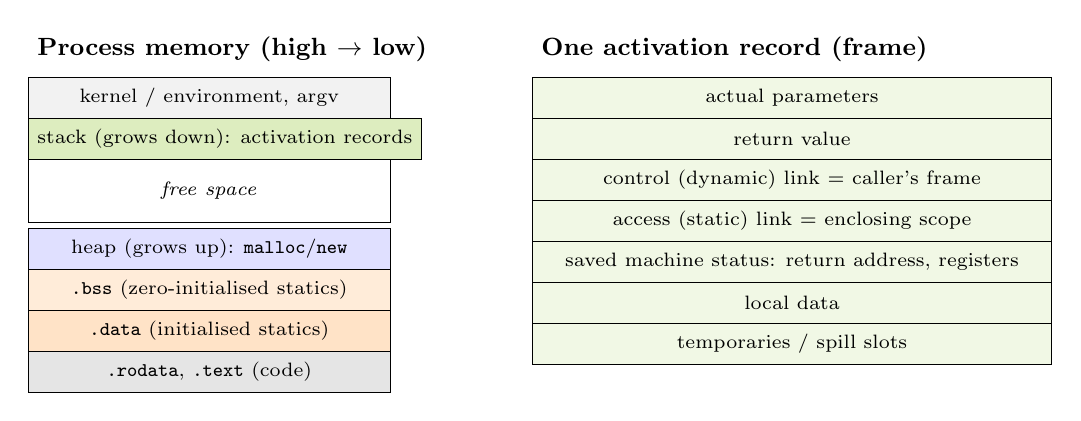
\begin{tikzpicture}[font=\scriptsize,cell/.style={draw,minimum width=4.6cm,minimum height=5.2mm,anchor=north west}]
\node[font=\small\bfseries,anchor=west] at (0,0.35) {Process memory (high $\to$ low)};
\node[cell,fill=black!5] at (0,0)       (c1) {kernel / environment, argv};
\node[cell,fill=nvgreen!25] at (0,-0.52) (c2) {stack (grows down): activation records};
\node[cell,fill=white,minimum height=8mm] at (0,-1.04) (c3) {\emph{free space}};
\node[cell,fill=blue!12] at (0,-1.92)  (c4) {heap (grows up): \texttt{malloc}/\texttt{new}};
\node[cell,fill=orange!15] at (0,-2.44) (c5) {\texttt{.bss} (zero-initialised statics)};
\node[cell,fill=orange!22] at (0,-2.96) (c6) {\texttt{.data} (initialised statics)};
\node[cell,fill=black!10] at (0,-3.48) (c7) {\texttt{.rodata}, \texttt{.text} (code)};
\node[font=\small\bfseries,anchor=west] at (6.4,0.35) {One activation record (frame)};
\foreach \y/\lbl in {0/{actual parameters},-0.52/{return value},-1.04/{control (dynamic) link = caller's frame},-1.56/{access (static) link = enclosing scope},-2.08/{saved machine status: return address, registers},-2.6/{local data},-3.12/{temporaries / spill slots}}
  \node[cell,minimum width=6.6cm,fill=nvgreen!10] at (6.4,\y) {\lbl};
\end{tikzpicture}
\end{center}
\begin{mustbox}
\begin{itemize}[nosep]
\item A \textbf{calling sequence} splits work between \emph{caller} (evaluate and pass arguments, save caller-saved registers, \texttt{call}) and \emph{callee} (prologue: push frame pointer, allocate locals; epilogue: restore, return). Frames form a stack because calls nest; a frame lives exactly as long as its call.
\item \textbf{Nested procedures} (Pascal, Python closures, GCC nested functions) need the \textbf{access link} (follow $k$ links to reach a variable $k$ scopes out) or a \textbf{display} (array indexed by nesting depth: $O(1)$ access, but updated on every call). C has no nested functions, so it needs neither.
\item \textbf{Tail-call optimisation:} a call in tail position (\texttt{return f(x);}) can reuse the caller's frame, turning recursion into a loop; guaranteed in Scheme, optional in C/C++ compilers, absent in CPython.
\item \textbf{Stack overflow} = unbounded recursion; \textbf{dangling reference} = pointer into a frame that has returned.
\end{itemize}
\end{mustbox}
\subsection{Parameter-passing mechanisms: the classic \texttt{swap(i, a[i])} question}
\begin{center}\small
\begin{tabularx}{\textwidth}{@{}L{2.7cm}Y@{}}
\toprule
\textbf{Mechanism} & \textbf{Semantics}\\
\midrule
call by value & callee gets a \emph{copy} of the value; changes are invisible to the caller (C, Java primitives)\\
call by reference & callee gets the \emph{address} (alias); the address of the actual is computed \textbf{once, at the call} (C++ \texttt{T\&}, Fortran)\\
copy-restore (value-result) & copy in at call, copy out at return to the addresses fixed at the call\\
call by name & the actual parameter is a \emph{thunk} re-evaluated at \textbf{every use} in the caller's environment (Algol 60, macros; Jensen's device)\\
\bottomrule
\end{tabularx}
\end{center}
\needspace{5\baselineskip}
\begin{lstlisting}[language={Python},title={swap(x, y) called as swap(i, a[i]) with i=1, a[1]=10, a[2]=20}]
def fresh(): return {"i": 1}, {1: 10, 2: 20, 10: 99}      # a[10] exists only so call-by-name has somewhere to write

def by_value():
    s, a = fresh(); x, y = s["i"], a[s["i"]]; t = x; x = y; y = t     # callee works on copies
    return s["i"], a
def by_reference():
    s, a = fresh(); idx = s["i"]                                       # address of a[i] fixed at the call
    t = s["i"]; s["i"] = a[idx]; a[idx] = t
    return s["i"], a
def by_value_result():
    s, a = fresh(); idx = s["i"]; x, y = s["i"], a[idx]                # copy in
    t = x; x = y; y = t
    s["i"] = x; a[idx] = y                                              # copy out to the addresses fixed at the call
    return s["i"], a
def by_name():
    s, a = fresh()
    x_get = lambda: s["i"];     x_set = lambda v: s.__setitem__("i", v)
    y_get = lambda: a[s["i"]];  y_set = lambda v: a.__setitem__(s["i"], v)   # a[i] re-evaluated at every use
    t = x_get(); x_set(y_get()); y_set(t)
    return s["i"], a

for name, f in (("value", by_value), ("reference", by_reference), ("value-result", by_value_result), ("name", by_name)):
    i, a = f(); print("%-13s i=%-2d a[1]=%-2d a[2]=%-2d a[10]=%d" % (name, i, a[1], a[2], a[10]))
\end{lstlisting}
\needspace{5\baselineskip}
\begin{lstlisting}[style=out,title={Answer: captured output}]
value         i=1  a[1]=10 a[2]=20 a[10]=99
reference     i=10 a[1]=1  a[2]=20 a[10]=99
value-result  i=10 a[1]=1  a[2]=20 a[10]=99
name          i=10 a[1]=10 a[2]=20 a[10]=1
\end{lstlisting}
\textbf{Why call-by-name differs:} after \texttt{x = y} sets \texttt{i} to 10, the later \texttt{y = t} re-evaluates \texttt{a[i]} as \texttt{a[10]}, so it writes the wrong element, while by reference the address \texttt{a[1]} was frozen at the call.

\subsection{Heap management and garbage collection}
\begin{center}\small
\begin{tabularx}{\textwidth}{@{}L{3.1cm}Y@{}}
\toprule
\textbf{Technique} & \textbf{Key facts}\\
\midrule
Free-list allocation & first fit (fast), best fit (least waste, slow, tiny fragments), worst fit; \textbf{coalescing} adjacent free blocks fights \emph{external} fragmentation; rounding sizes causes \emph{internal} fragmentation; segregated lists (size classes) are the practical choice\\
Reference counting & count pointers to each object, free at zero; immediate, incremental; \textbf{cannot reclaim cycles}; overhead on every pointer store (CPython, Swift ARC, \texttt{shared\_ptr})\\
Mark-and-sweep & mark everything reachable from roots (stack, registers, globals), sweep the rest; handles cycles; cost $\propto$ heap size; leaves fragmentation; ``stop the world''\\
Copying (semi-space, Cheney) & copy live objects to a fresh space; cost $\propto$ live data; compacts, allocation is a pointer bump; wastes half the memory\\
Generational & most objects die young: collect the nursery often, the old generation rarely; needs a write barrier\\
Conservative (Boehm) & treats any word that looks like a pointer as one; works for C/C++ but can retain garbage\\
\bottomrule
\end{tabularx}
\end{center}

\section{Lab: a complete mini compiler in 250 lines \prio{2}}
\label{sec:lab}
Interviewers who ask about ``compiler projects'' love candidates who built the whole pipeline once. This one (source in Appendix~\ref{app:tiny}) is also the \emph{system under test} in Chapter~\ref{ch:lab}. Language: integer variables, arithmetic, comparisons, \texttt{\&\&} \texttt{||} \texttt{!}, \texttt{if/else}, \texttt{while}, \texttt{print}; division truncates toward zero and division by zero traps.
\textbf{Pipeline:} regex lexer $\to$ recursive descent + precedence climbing parser $\to$ AST $\to$ TAC with jumping code $\to$ optimiser (constant folding/propagation, algebraic simplification, local CSE, dead-code elimination, jump clean-up, branch inversion, temp coalescing) $\to$ TAC virtual machine; a separate \textbf{reference interpreter} over the AST serves as the semantic oracle.
\needspace{5\baselineskip}
\begin{lstlisting}[language={Python},title={Front end: tokens and AST (note how precedence shapes the tree)}]
import tiny
print(tiny.lex("x = 1 + 2 * 3;")[:-1])
print(tiny.parse("x = 1 + 2 * 3;"))
print(tiny.parse("y = a - b - c;"))          # left-associative: (a - b) - c
\end{lstlisting}
\needspace{5\baselineskip}
\begin{lstlisting}[style=out,title={Captured output}]
[('id', 'x'), ('op', '='), ('num', 1), ('op', '+'), ('num', 2), ('op', '*'), ('num', 3), ('op', ';')]
('block', [('assign', 'x', ('bin', '+', ('num', 1), ('bin', '*', ('num', 2), ('num', 3))))])
('block', [('assign', 'y', ('bin', '-', ('bin', '-', ('var', 'a'), ('var', 'b')), ('var', 'c')))])
\end{lstlisting}
\needspace{5\baselineskip}
\begin{lstlisting}[language={Python},title={TAC with jumping code for the loop, before and after optimisation}]
import tiny
SRC = """n = 10; s = 0; i = 1;
while (i <= n) {
  if (i % 2 == 0 && i > 2) { s = s + i * 2; } else { s = s + i; }
  i = i + 1;
}
print(s);"""
raw = tiny.compile_source(SRC, opt=False)
opt = tiny.compile_source(SRC, opt=True)
print("=== raw TAC (%d instructions)" % len([i for i in raw if i[0] != "label"]));       print(tiny.show(raw))
print("=== optimised TAC (%d instructions)" % len([i for i in opt if i[0] != "label"]));  print(tiny.show(opt))
ref = tiny.interpret(tiny.parse(SRC))
r1, r2 = tiny.run_tac(raw), tiny.run_tac(opt)
print("reference interpreter:", ref)
print("raw TAC on the VM    :", r1[:2], "executed", r1[2], "instructions")
print("optimised TAC on VM  :", r2[:2], "executed", r2[2], "instructions")
\end{lstlisting}
\needspace{5\baselineskip}
\begin{lstlisting}[style=out,title={Captured output}]
=== raw TAC (20 instructions)
    n = 10
    s = 0
    i = 1
L1:
    if i <= n goto L2
    goto L3
L2:
    t1 = i % 2
    if t1 == 0 goto L7
    goto L5
L7:
    if i > 2 goto L4
    goto L5
L4:
    t2 = i * 2
    t3 = s + t2
    s = t3
    goto L6
L5:
    t4 = s + i
    s = t4
L6:
    t5 = i + 1
    i = t5
    goto L1
L3:
    print s
=== optimised TAC (14 instructions)
    n = 10
    s = 0
    i = 1
L1:
    if i > n goto L3
    t1 = i % 2
    if t1 != 0 goto L5
    if i <= 2 goto L5
    t2 = i * 2
    s = s + t2
    goto L6
L5:
    s = s + i
L6:
    i = i + 1
    goto L1
L3:
    print s
reference interpreter: ([83], None)
raw TAC on the VM    : ([83], None) executed 105 instructions
optimised TAC on VM  : ([83], None) executed 78 instructions
\end{lstlisting}
\textbf{Observe:} (1) \texttt{i \% 2 == 0 \&\& i > 2} became two conditional jumps: there is no \texttt{\&\&} at run time. (2) After branch inversion the pattern \texttt{if c goto A; goto B; A:} became \texttt{if !c goto B}. (3) Temporaries were coalesced (\texttt{t3 = s + t2; s = t3} became \texttt{s = s + t2}). (4) Same output (83) from all three executors, with fewer executed instructions.
\needspace{5\baselineskip}
\begin{lstlisting}[language={Python},title={Local CSE and constant folding}]
import tiny
cse = "a = b * -c + b * -c; print(a);"
print("--- CSE: raw");  print(tiny.show(tiny.compile_source(cse, opt=False)))
print("--- CSE: optimised (the second b * -c is reused: the DAG idea)"); print(tiny.show(tiny.compile_source(cse)))
print(tiny.interpret(tiny.parse(cse), env0={"b": 3, "c": 4}), tiny.run_tac(tiny.compile_source(cse), env0={"b": 3, "c": 4})[:2])
cf = "x = 2 * 3 + 4; y = x * 1; z = y + 0; print(z / 2); if (x > 5 || z < 0) { print(1); } else { print(0); }"
print("--- constant folding + dead branch: raw has %d instructions, optimised:" % len([i for i in tiny.compile_source(cf, opt=False) if i[0] != "label"]))
print(tiny.show(tiny.compile_source(cf)))
\end{lstlisting}
\needspace{5\baselineskip}
\begin{lstlisting}[style=out,title={Captured output}]
--- CSE: raw
    t1 = -c
    t2 = b * t1
    t3 = -c
    t4 = b * t3
    t5 = t2 + t4
    a = t5
    print a
--- CSE: optimised (the second b * -c is reused: the DAG idea)
    t1 = -c
    t2 = b * t1
    t5 = t2 + t2
    print t5
([-24], None) ([-24], None)
--- constant folding + dead branch: raw has 16 instructions, optimised:
    print 5
    print 1
\end{lstlisting}

\section{Practice \prio{3}}
\begin{qn}For the grammar $E\to E+T\mid T$, $T\to T*F\mid F$, $F\to\textit{digit}$ with $F.val=\textit{digit}.lexval$ etc., what is \texttt{E.val} for \texttt{3*5+4}?\end{qn}
\begin{ans}19: $T.val=3\cdot5=15$, $E.val=15+4$. (S-attributed: computed bottom-up.)\end{ans}
\begin{qn}Which is true: (a) synthesised attributes may depend on siblings; (b) L-attributed SDDs can be evaluated during top-down parsing; (c) every S-attributed SDD is L-attributed?\end{qn}
\begin{ans}(b) and (c). (a) is false: synthesised attributes depend on children (and the node itself) only.\end{ans}
\begin{qn}Translate \texttt{x = a[i] + b} to three-address code if \texttt{a} is an \texttt{int} array.\end{qn}
\begin{ans}\texttt{t1 = i * 4; t2 = a[t1]; t3 = t2 + b; x = t3}. (Scaling by the element width; in real IRs this is an address computation then a load.)\end{ans}
\begin{qn}A procedure is called with arguments by name vs.\ reference: when do results differ?\end{qn}
\begin{ans}When the actual parameter's \emph{expression} depends on a variable that the procedure modifies (\texttt{a[i]} with \texttt{i} changed): by name re-evaluates it at each use; by reference fixed the address at the call (see the swap output).\end{ans}
\begin{qn}Why does SSA place $\varphi$ functions at dominance frontiers?\end{qn}
\begin{ans}A definition of $v$ in block $B$ reaches every block $B$ dominates unambiguously. Just outside that region (the dominance frontier) another definition may also reach, so the value becomes path-dependent: exactly where a $\varphi$ is needed. Iterating covers the new definitions created by the $\varphi$s themselves.\end{ans}
\begin{qn}Which GC can reclaim a cycle of two objects that point to each other: reference counting or mark-and-sweep?\end{qn}
\begin{ans}Mark-and-sweep (the cycle is unreachable from roots). Reference counting leaves both counts at 1 (the \texttt{shared\_ptr} cycle leak seen in Chapter~\ref{ch:cpp}).\end{ans}


% ===== 11-optimization.tex.in =====
\chapter{Optimisation, Code Generation and Linking}
\label{ch:opt}

\begin{chapbox}
\textbf{Priority \prio{3}. Time: 100 min.} This is where compiler interviews concentrate (S2, S4, S6, S8, S10): loop unrolling, inlining, data-flow and dependence analysis, pointer analysis, matrix-multiplication optimisations, graph-colouring register allocation.
Every analysis result below is produced by code in the book (Appendices~\ref{app:tiny}--\ref{app:backend}); the experiments (assembly, vectoriser remarks, timings, linker errors) are real tool output.
\end{chapbox}




\section{What an optimiser is allowed to do \prio{3}}
\begin{mustbox}
\begin{itemize}[nosep]
\item \textbf{The as-if rule:} the compiler may transform the program in any way as long as the \emph{observable behaviour} (I/O, volatile accesses, and the results of well-defined programs) is unchanged. \textbf{Legality} = the analysis proves the transformation safe; \textbf{profitability} = a cost model predicts it helps. Many bugs are legality bugs (wrong analysis); many missed speed-ups are profitability judgements.
\item \textbf{UB is the optimiser's licence:} because signed overflow, out-of-bounds access and aliasing violations ``cannot happen'', loops can be widened, checks removed, loads reordered (Chapter~\ref{ch:c}, Section~\ref{sec:ub}).
\item \textbf{Levels (GCC/Clang):} \texttt{-O0} none (debuggable); \texttt{-O1} cheap clean-ups; \texttt{-O2} the default for releases (no large code growth); \texttt{-O3} adds aggressive loop transforms, vectorisation, larger inlining; \texttt{-Os/-Oz} optimise for size; \texttt{-Ofast} = \texttt{-O3} plus \texttt{-ffast-math} (breaks IEEE semantics: assumes no NaN/Inf, allows reassociation); \texttt{-Og} GCC's debug-friendly level.
\item \textbf{Phase ordering problem:} optimisations enable and disable each other (inlining enables constant propagation, which enables dead-code elimination, which shrinks the function so it is inlined elsewhere); no single order is best, so pipelines run \emph{cleanup} passes repeatedly. Whether a transformation is machine-independent (on IR) or machine-dependent (peephole, scheduling, register allocation) decides where it sits.
\end{itemize}
\end{mustbox}

\section{Local optimisations (within a basic block) \prio{3}}
\begin{center}\small
\begin{tabularx}{\textwidth}{@{}L{3.9cm}Y@{}}
\toprule
\textbf{Optimisation} & \textbf{Example}\\
\midrule
Constant folding & \texttt{x = 2 * 3 + 4} $\to$ \texttt{x = 10}; careful: fold with the \emph{target's} semantics (integer division, overflow, floating-point rounding)\\
Constant / copy propagation & after \texttt{y = x; z = y + 1} use \texttt{x} directly; after \texttt{c = 5} replace uses of \texttt{c} by 5\\
Algebraic simplification & \texttt{x+0}, \texttt{x*1}, \texttt{x*0}, \texttt{x-x}, \texttt{x\&0}; (not for floating point without \texttt{-ffast-math}: \texttt{x*0} may be NaN)\\
\textbf{Strength reduction} & replace an expensive operation by a cheaper equivalent: \texttt{x*8} $\to$ shift/\texttt{lea}, \texttt{x/2\textasciicircum{}k} $\to$ shift with fix-up, \texttt{x\%16} $\to$ \texttt{and}\\
Common subexpression elimination (CSE) / \textbf{value numbering} & compute \texttt{b * -c} once and reuse; value numbering assigns equal numbers to equal computations using a hash table\\
Dead-code elimination & delete instructions whose results are never used and have no side effects; \emph{dead stores}; unreachable blocks\\
Peephole optimisation & slide a small window over generated code: remove \texttt{mov r,r}, jump-to-next, \texttt{push/pop} pairs, replace sequences by one idiom\\
\bottomrule
\end{tabularx}
\end{center}
Strength reduction in real compiler output (GCC \texttt{-O2}, x86-64). Note that signed \texttt{x/2} is \emph{not} a plain shift: negative odd values must round toward zero.
\begin{lstlisting}[language={C}]
int mul9(int x)             { return x * 9; }
int mul8(int x)             { return x * 8; }
unsigned udiv8(unsigned x)  { return x / 8; }
int sdiv2(int x)            { return x / 2; }
unsigned umod16(unsigned x) { return x % 16; }
int times1000(int x)        { return x * 1000; }
\end{lstlisting}
\begin{lstlisting}[style=shcmd]
$ gcc -O2 -S -masm=intel sr.c
\end{lstlisting}
\begin{lstlisting}[style=out]
mul9:
    lea    eax, [rdi+rdi*8]
    ret
mul8:
    lea    eax, 0[0+rdi*8]
    ret
udiv8:
    mov    eax, edi
    shr    eax, 3
    ret
sdiv2:
    mov    eax, edi
    shr    eax, 31
    add    eax, edi
    sar    eax
    ret
umod16:
    mov    eax, edi
    and    eax, 15
    ret
times1000:
    imul    eax, edi, 1000
    ret
\end{lstlisting}
\textbf{Reading it:} \texttt{x*9} is \texttt{x + 8x}, one \texttt{lea}; \texttt{x*8} is a scaled address computation; unsigned \texttt{x/8} is \texttt{shr 3}; \texttt{x\%16} is \texttt{and 15}; signed \texttt{x/2} adds the sign bit (\texttt{shr 31}) before the arithmetic shift (\texttt{sar}) to round toward zero; \texttt{x*1000} stays a real \texttt{imul} (no cheaper form). This is also where \emph{compiler verification} lives: every one of these rewrites must be exactly right for \emph{all} inputs, including \texttt{INT\_MIN}.

\section{Data-flow analysis \prio{3}}
\begin{mustbox}[The framework]
A data-flow problem assigns each basic block $B$ a set $IN[B]$ and $OUT[B]$ satisfying equations built from per-block \textbf{gen}/\textbf{kill} sets. The solution is the \emph{fixed point} of iterating them; it terminates because the transfer functions are \emph{monotone} on a lattice of finite height. Processing blocks in \textbf{reverse post-order} (forward problems) or post-order (backward) converges in few passes (roughly the loop-nesting depth plus two).
\begin{center}\small
\begin{tabularx}{\textwidth}{@{}L{2.9cm}L{1.9cm}L{1.7cm}Y@{}}
\toprule
\textbf{Analysis} & \textbf{Direction} & \textbf{Meet} & \textbf{Equations / used for}\\
\midrule
\textbf{Reaching definitions} & forward & $\cup$ (may) & $OUT=gen\cup(IN-kill)$, $IN=\bigcup_{P}OUT[P]$; constant/copy propagation, loop invariants, uninitialised-use warnings\\
\textbf{Live variables} & backward & $\cup$ (may) & $IN=use\cup(OUT-def)$, $OUT=\bigcup_{S}IN[S]$; \textbf{register allocation}, dead-code elimination\\
\textbf{Available expressions} & forward & $\cap$ (must) & $OUT=gen\cup(IN-kill)$, $IN=\bigcap_{P}OUT[P]$, init all non-entry to $U$; \textbf{global CSE}\\
Very busy expressions & backward & $\cap$ (must) & code hoisting, partial-redundancy elimination (PRE)\\
\bottomrule
\end{tabularx}
\end{center}
\textbf{May} analyses ask ``is it \emph{possible}?'' (union at joins; initialise to $\emptyset$); \textbf{must} analyses ask ``is it \emph{certain} on every path?'' (intersection; initialise to the universe).
\end{mustbox}
\needspace{5\baselineskip}
\begin{lstlisting}[language={Python},title={Reaching definitions and live variables on the loop CFG (iterated to a fixed point)}]
import dataflow
dataflow.report("""n = 10; s = 0; i = 1;
while (i <= n) {
  if (i % 2 == 0 && i > 2) { s = s + i * 2; } else { s = s + i; }
  i = i + 1;
}
print(s);""", which=("rd", "live"))
\end{lstlisting}
\needspace{5\baselineskip}
\begin{lstlisting}[style=out,title={Captured output}]
Basic blocks:
  B0: n = 10; s = 0; i = 1                           -> [1]
  B1: L1:; if i > n goto L3                          -> [7, 2]
  B2: t1 = i % 2; if t1 != 0 goto L5                 -> [5, 3]
  B3: if i <= 2 goto L5                              -> [5, 4]
  B4: t2 = i * 2; s = s + t2; goto L6                -> [6]
  B5: L5:; s = s + i                                 -> [6]
  B6: L6:; i = i + 1; goto L1                        -> [1]
  B7: L3:; print s                                   -> []

Reaching definitions (forward, union) -- stable after 3 passes
  definitions: d1:n@B0  d2:s@B0  d3:i@B0  d4:t1@B2  d5:t2@B4  d6:s@B4  d7:s@B5  d8:i@B6
  B0  gen={d1,d2,d3}   kill={d6,d7,d8}       IN={}                     OUT={d1,d2,d3}
  B1  gen={}           kill={}               IN={d1,d2,d3,d4,d5,d6,d7,d8} OUT={d1,d2,d3,d4,d5,d6,d7,d8}
  B2  gen={d4}         kill={}               IN={d1,d2,d3,d4,d5,d6,d7,d8} OUT={d1,d2,d3,d4,d5,d6,d7,d8}
  B3  gen={}           kill={}               IN={d1,d2,d3,d4,d5,d6,d7,d8} OUT={d1,d2,d3,d4,d5,d6,d7,d8}
  B4  gen={d5,d6}      kill={d2,d7}          IN={d1,d2,d3,d4,d5,d6,d7,d8} OUT={d1,d3,d4,d5,d6,d8}
  B5  gen={d7}         kill={d2,d6}          IN={d1,d2,d3,d4,d5,d6,d7,d8} OUT={d1,d3,d4,d5,d7,d8}
  B6  gen={d8}         kill={d3}             IN={d1,d3,d4,d5,d6,d7,d8} OUT={d1,d4,d5,d6,d7,d8}
  B7  gen={}           kill={}               IN={d1,d2,d3,d4,d5,d6,d7,d8} OUT={d1,d2,d3,d4,d5,d6,d7,d8}

Live variables (backward, union) -- stable after 3 passes
  B0  use={}         def={i,n,s}    IN={}             OUT={i,n,s}
  B1  use={i,n}      def={}         IN={i,n,s}        OUT={i,n,s}
  B2  use={i}        def={t1}       IN={i,n,s}        OUT={i,n,s}
  B3  use={i}        def={}         IN={i,n,s}        OUT={i,n,s}
  B4  use={i,s}      def={s,t2}     IN={i,n,s}        OUT={i,n,s}
  B5  use={i,s}      def={s}        IN={i,n,s}        OUT={i,n,s}
  B6  use={i}        def={i}        IN={i,n,s}        OUT={i,n,s}
  B7  use={s}        def={}         IN={s}            OUT={}
\end{lstlisting}
\begin{exbox}[How to read it]
\begin{itemize}[nosep]
\item $d_2$ (\texttt{s = 0}) reaches the loop header B1 (first iteration) but is killed on \emph{both} arms of the \texttt{if} (B4 defines $d_6$, B5 defines $d_7$), so it is absent from $IN[B6]$. Every in-loop definition reaches B1 through the back edge.
\item Live variables flow \emph{backwards}: B7 uses \texttt{s}, so \texttt{s} is live out of B1; \texttt{n} is live throughout the loop because B1 re-reads it; \texttt{t1} and \texttt{t2} are never live across a block boundary: they could live in a register that is reused. Both analyses stabilised in 3 passes.
\end{itemize}
\end{exbox}
\textbf{Available expressions and global CSE.} In the program below \texttt{a + b} is computed in B0, again on one branch, and again at the join. Is the third computation redundant?
\begin{lstlisting}[language={Python}]
import dataflow
dataflow.report("""x = a + b;
if (c) { y = a + b; } else { z = a * b; }
w = a + b;
print(x + y + z + w);""", which=("avail",))
\end{lstlisting}
\needspace{5\baselineskip}
\begin{lstlisting}[style=out,title={Captured output}]
Basic blocks:
  B0: x = a + b; if c == 0 goto L2                   -> [2, 1]
  B1: y = a + b; goto L3                             -> [3]
  B2: L2:; z = a * b                                 -> [3]
  B3: L3:; t4 = a + b; t5 = x + y; t6 = t5 + z; t7 = t6 + t4; print t7 -> []

Available expressions (forward, intersection) -- stable after 2 passes
  B0  gen={a + b}                IN={}                       OUT={a + b}
  B1  gen={a + b}                IN={a + b}                  OUT={a + b}
  B2  gen={a * b}                IN={a + b}                  OUT={a * b, a + b}
  B3  gen={a + b, t5 + z, t6 + t4, x + y} IN={a + b}                  OUT={a + b, t5 + z, t6 + t4, x + y}
\end{lstlisting}
\textbf{Why:} $IN[B3]=OUT[B1]\cap OUT[B2]=\{a+b\}\cap\{a*b,\ a+b\}=\{a+b\}$. The expression is available on \emph{every} path into the join, so the third \texttt{a + b} can be replaced by a copy of the earlier value (global CSE). \texttt{a * b} is not available (only one path computes it). Local value numbering alone could not see this because the computations live in different blocks.
\begin{trapbox}[Facts to quote]
Bit-vector frameworks (the four above) are \emph{distributive}, so the iterative \emph{maximal fixed point} equals the \emph{meet-over-all-paths} ideal. \textbf{Constant propagation} is monotone but \emph{not} distributive (the join of $x{=}2,y{=}3$ and $x{=}3,y{=}2$ loses $x{+}y{=}5$), so it needs a richer lattice (constant / $\top$ / $\bot$). Iteration order matters for speed, never for the result. Inter-procedural data-flow needs call-graph and context-sensitivity decisions.
\end{trapbox}

\section{Loop optimisations and dependence analysis \prio{3}}
\begin{defbox}[Natural loops]
A \textbf{back edge} is an edge $n\to h$ where $h$ dominates $n$. The \textbf{natural loop} of that edge is $h$ plus all nodes that can reach $n$ without passing through $h$; $h$ is the \textbf{header}. Loops are the hot spots, so most optimisations target them. A \textbf{pre-header} block before the header is where hoisted code is placed.
\end{defbox}
\begin{center}\small
\begin{tabularx}{\textwidth}{@{}L{3.5cm}Y@{}}
\toprule
\textbf{Transformation} & \textbf{What it does, when it is legal, why it helps}\\
\midrule
\textbf{Loop-invariant code motion (LICM)} & hoist computations whose operands do not change in the loop to the pre-header. Legal if the instruction cannot trap or execute speculatively unsafely (e.g.\ a division needs a guard), and its value is not used before definition\\
\textbf{Induction-variable strength reduction / elimination} & replace \texttt{a[i*4]} address arithmetic by a pointer incremented by 4 per iteration; eliminate a second induction variable that tracks the first\\
\textbf{Loop unrolling} & replicate the body $k$ times (plus a remainder loop). \emph{Helps:} fewer branch and counter instructions, more instruction-level parallelism, enables scheduling, CSE across iterations and vectorisation. \emph{Costs:} larger code (I-cache pressure), more register pressure. Compiler decides by trip count and body size\\
Loop peeling / unswitching & peel the first iterations (to remove an iteration-dependent special case); move a loop-invariant \texttt{if} outside the loop (duplicating the loop)\\
Loop fusion / fission & merge adjacent loops over the same range (fewer passes over memory) / split a loop (enables vectorising part of it, reduces pressure)\\
\textbf{Loop interchange} & swap nested loop order to make the innermost loop access memory with stride 1 (legal only if no dependence direction vector is reversed)\\
\textbf{Tiling (blocking)} & split iteration space into blocks that fit in cache/registers/shared memory, reusing data before eviction\\
\textbf{Vectorisation} & turn $n$ scalar iterations into SIMD operations; needs no loop-carried dependence (or a recognised reduction) and known/checked aliasing\\
Software pipelining & overlap iterations in the schedule (VLIW/DSP, GPUs' asynchronous copies)\\
\bottomrule
\end{tabularx}
\end{center}
\needspace{5\baselineskip}
\begin{lstlisting}[language={Python},title={Natural loop and loop-invariant instruction detection (uses reaching definitions)}]
import dataflow
dataflow.report("""a = k + 1; b = 7; s = 0; i = 0;
while (i < n) { c = a * b; s = s + c + i; i = i + 1; }
print(s);""", which=("loops",))
\end{lstlisting}
\needspace{5\baselineskip}
\begin{lstlisting}[style=out,title={Captured output}]
Basic blocks:
  B0: a = k + 1; b = 7; s = 0; i = 0                 -> [1]
  B1: L1:; if i >= n goto L3                         -> [3, 2]
  B2: t2 = a * b; t3 = s + t2; s = t3 + i; i = i + 1; goto L1 -> [1]
  B3: L3:; print s                                   -> []

Natural loop with header B1, body [1, 2]
  loop-invariant instructions: ['t2 = a * b  (B2)']
\end{lstlisting}
\textbf{Why:} \texttt{t2 = a * b} is invariant: \texttt{a} and \texttt{b} have all their reaching definitions \emph{outside} the loop (B0). \texttt{s + t2} and \texttt{i + 1} are not: \texttt{s} and \texttt{i} are redefined inside the loop. LICM would move the multiplication to the pre-header, saving one instruction per iteration. \texttt{k} and \texttt{n} are program inputs (no definition at all), hence invariant.

\subsection{Dependences decide legality}
\begin{mustbox}
For two statements touching the same memory: \textbf{flow (true, RAW)}: write then read; \textbf{anti (WAR)}: read then write; \textbf{output (WAW)}: write then write. Only \emph{flow} dependences carry real data; anti/output can be removed by renaming. A dependence is \textbf{loop-carried} if source and sink are in different iterations; its \textbf{distance} is the iteration difference (the direction vector gives the sign). A loop can be \emph{parallelised or vectorised} when it has no loop-carried dependence (reductions excepted). \textbf{Loop interchange} is legal iff no dependence's direction vector becomes lexicographically negative.
\textbf{GCD test:} for \texttt{a[c1*i+k1] = ... a[c2*j+k2]}, a dependence is possible only if $\gcd(c_1,c_2)\mid(k_2-k_1)$. It ignores loop bounds, so it may report a dependence that does not exist, but never misses one (a \emph{conservative} test).
\end{mustbox}
\needspace{5\baselineskip}
\begin{lstlisting}[language={Python},title={GCD test versus brute-force enumeration of the iteration space}]
from math import gcd
def gcd_test(c1, k1, c2, k2): return (k2 - k1) % gcd(c1, c2) == 0              # write a[c1*i+k1], read a[c2*j+k2]
def brute(c1, k1, c2, k2, n=60):
    pairs = {(i, j) for i in range(n) for j in range(n) if c1 * i + k1 == c2 * j + k2}
    return bool(pairs), sorted({j - i for i, j in pairs}, key=abs)[:3]
cases = [("a[i]   = a[i-1] + 1", 1, 0, 1, -1), ("a[2*i] = a[2*i+1]", 2, 0, 2, 1),
         ("a[i]   = a[i] + 1", 1, 0, 1, 0), ("a[2*i] = a[4*j+2]", 2, 0, 4, 2), ("a[3*i] = a[6*j+1]", 3, 0, 6, 1)]
print("%-22s %-10s %-24s" % ("loop", "GCD test", "brute force (distances j-i)"))
for text, c1, k1, c2, k2 in cases:
    exists, dist = brute(c1, k1, c2, k2)
    print("%-22s %-10s %s %s" % (text, "may depend" if gcd_test(c1, k1, c2, k2) else "independent", "dependent" if exists else "independent", dist))
\end{lstlisting}
\needspace{5\baselineskip}
\begin{lstlisting}[style=out,title={Captured output}]
loop                   GCD test   brute force (distances j-i)
a[i]   = a[i-1] + 1    may depend dependent [1]
a[2*i] = a[2*i+1]      independent independent []
a[i]   = a[i] + 1      may depend dependent [0]
a[2*i] = a[4*j+2]      may depend dependent [-1, -2, -3]
a[3*i] = a[6*j+1]      independent independent []
\end{lstlisting}
\textbf{Reading it:} \texttt{a[i] = a[i-1] + 1} has distance $+1$: a loop-carried flow dependence (each iteration needs the previous result), so it cannot be vectorised or run in parallel. \texttt{a[2*i] = a[2*i+1]} writes even and reads odd elements: provably independent. \texttt{a[i] = a[i] + 1} has distance 0 (loop-independent). The fourth loop's distance is \emph{not constant} ($-1,-2,-3,\ldots$: reads at iteration $j$ precede the overwrite at iteration $2j+1$, an anti-dependence), so legality of vectorisation/interchange needs a more precise test (Banerjee, Omega); the fifth is independent by the GCD test. The GCD test never missed a real dependence here.

\subsection{What a real vectoriser says (Clang remarks, real output)}
\begin{lstlisting}[language={C}]
void add_arrays(int *a, const int *b, const int *c, int n) { for (int i = 0; i < n; i++) a[i] = b[i] + c[i]; }
void recurrence(int *a, int n)                              { for (int i = 1; i < n; i++) a[i] = a[i-1] + 1; }
int  sum(const int *a, int n)                               { int s = 0; for (int i = 0; i < n; i++) s += a[i]; return s; }
\end{lstlisting}
\begin{lstlisting}[style=shcmd]
$ clang -O2 -c vec.c -Rpass=loop-vectorize -Rpass-missed=loop-vectorize -Rpass=loop-unroll
\end{lstlisting}
\begin{lstlisting}[style=out]
line 1: remark: unrolled loop by a factor of 4 with run-time trip count [-Rpass=loop-unroll]
line 2: remark: loop not vectorized [-Rpass-missed=loop-vectorize]
line 2: remark: unrolled loop by a factor of 4 with run-time trip count [-Rpass=loop-unroll]
\end{lstlisting}
\textbf{Reading it:} line 1 and 3 vectorised (4 ints per SIMD register, interleaved by 2; the reduction on line 3 is recognised); line 2 is \emph{not} vectorised because of the loop-carried dependence; the scalar remainder loops were unrolled by 4. These remarks are the first tool to use when asked ``why is my loop slow?'' or ``why did the optimiser not fire?''. Note that \texttt{add\_arrays} may alias (\texttt{a} could overlap \texttt{b}), so the vectoriser emits a \emph{run-time alias check}; \texttt{restrict} removes the need.

\subsection{Matrix multiplication ``and all applicable optimisations'' (S6): a measured answer}
The full answer to the Shanghai interview question is a \emph{list with reasons}: (1) \textbf{loop interchange} to make the innermost accesses stride-1; (2) \textbf{tiling} for cache reuse (and registers/shared memory on GPUs); (3) \textbf{register blocking} and \textbf{unrolling} to keep accumulators in registers and expose ILP; (4) \textbf{vectorisation}; (5) \textbf{multithreading} across output tiles; (6) \textbf{transposing} or packing \texttt{B} for contiguous access; (7) \textbf{prefetching}/software pipelining; (8) algorithmic: Strassen's $O(n^{2.81})$ for very large $n$; (9) use a tuned library (BLAS, cuBLAS) or Tensor Cores. Experiment (768$\times$768 doubles, GCC \texttt{-O2}, this sandbox; absolute times vary by machine, ratios are the lesson):
\needspace{5\baselineskip}
\begin{lstlisting}[language={C},title={Textbook order vs. loop interchange vs. tiling}]
#include <stdio.h>
#include <time.h>
#define N 768
static double A[N][N], B[N][N], C[N][N];
static double now(void) { struct timespec t; clock_gettime(CLOCK_MONOTONIC, &t); return t.tv_sec + t.tv_nsec * 1e-9; }
static void clear(void) { for (int i = 0; i < N; i++) for (int j = 0; j < N; j++) C[i][j] = 0; }
static double checksum(void) { double s = 0; for (int i = 0; i < N; i++) for (int j = 0; j < N; j++) s += C[i][j] * ((i + j) % 7 + 1); return s; }
static void mm_ijk(void) {                    /* B is walked down a column: stride N*8 bytes, a cache miss per access */
    for (int i = 0; i < N; i++) for (int j = 0; j < N; j++) { double s = 0; for (int k = 0; k < N; k++) s += A[i][k] * B[k][j]; C[i][j] = s; }
}
static void mm_ikj(void) {                    /* interchange: B and C walked along rows, vectorisable inner loop */
    for (int i = 0; i < N; i++) for (int k = 0; k < N; k++) { double a = A[i][k]; for (int j = 0; j < N; j++) C[i][j] += a * B[k][j]; }
}
#define BS 64
static void mm_tiled(void) {                  /* blocking: each 64x64 tile of B and C is reused while it is hot in cache */
    for (int ii = 0; ii < N; ii += BS) for (int kk = 0; kk < N; kk += BS) for (int jj = 0; jj < N; jj += BS)
        for (int i = ii; i < ii + BS; i++) for (int k = kk; k < kk + BS; k++) { double a = A[i][k]; for (int j = jj; j < jj + BS; j++) C[i][j] += a * B[k][j]; }
}
int main(void) {
    for (int i = 0; i < N; i++) for (int j = 0; j < N; j++) { A[i][j] = (i * 3 + j) % 10 * 0.5; B[i][j] = (i + j * 2) % 9 * 0.25; }
    void (*fn[])(void) = { mm_ijk, mm_ikj, mm_tiled };
    const char *name[] = { "ijk (textbook)", "ikj (interchange)", "tiled 64x64" };
    double base = 0;
    for (int v = 0; v < 3; v++) {
        clear(); double t0 = now(); fn[v](); double t = now() - t0;
        if (v == 0) base = t;
        printf("%-18s %6.2f s   speed-up %4.1fx   checksum %.1f\n", name[v], t, base / t, checksum());
    }
    return 0;
}
\end{lstlisting}
\needspace{5\baselineskip}
\begin{lstlisting}[style=out,title={Captured output (timings are measurements)}]
ijk (textbook)       0.49 s   speed-up  1.0x   checksum 4076851668.4
ikj (interchange)    0.14 s   speed-up  3.5x   checksum 4076851668.4
tiled 64x64          0.12 s   speed-up  4.2x   checksum 4076851668.4
\end{lstlisting}
\textbf{Reading it:} identical checksums (same arithmetic, same summation order per element: interchange and tiling are \emph{legal} here because they preserve the dependences). Interchange alone gives a multi-fold gain by turning cache misses into streaming accesses; tiling adds reuse. Floating-point note: transformations that change the \emph{order of additions} (parallel or vectorised reductions) change rounding, so compilers only do them with \texttt{-ffast-math} or explicit permission; verification tests must compare with a tolerance (Chapter~\ref{ch:verif}).

\subsection{Alias and pointer analysis (asked in S4)}
Optimisations need to know whether two pointers can refer to the same memory. \textbf{Results:} must-alias, may-alias, no-alias. \textbf{Sources of no-alias facts:} distinct local objects, \texttt{restrict}, C/C++ type-based alias analysis (an \texttt{int*} cannot alias a \texttt{float*}), \texttt{noalias} function attributes, GPU address spaces (shared vs.\ global never alias). \textbf{Points-to algorithms:} \emph{Andersen} (inclusion-based: each assignment $p=q$ adds $pts(q)\subseteq pts(p)$; precise, roughly $O(n^3)$) vs.\ \emph{Steensgaard} (unification-based: near-linear, less precise). \textbf{Flow-sensitive} (order matters) vs.\ \textbf{insensitive}; \textbf{context-sensitive} (distinguish call sites) vs.\ insensitive. Imprecise alias information is the main obstacle to vectorising C code.

\section{Interprocedural optimisation \prio{2}}
\begin{itemize}[nosep]
\item \textbf{Inlining:} replace a call by the callee's body. \emph{Benefits:} no call overhead, exposes constant propagation, CSE and dead-code elimination across the boundary (often the biggest win). \emph{Costs:} code growth, I-cache pressure, compile time. Heuristics: callee size, call-site hotness, \texttt{inline}/\texttt{always\_inline}/\texttt{noinline}. Recursion limits inlining.
\item \textbf{Tail-call elimination}, \textbf{devirtualisation} (turn a virtual call into a direct one when the dynamic type is known), \textbf{IPSCCP} (propagate constants across functions), \textbf{dead-argument elimination}, \textbf{function specialisation/cloning}.
\item \textbf{LTO/ThinLTO:} defer optimisation to link time so it sees the whole program; \textbf{PGO:} use measured branch/call frequencies to drive layout and inlining; \textbf{escape analysis:} an object that never escapes the function can live on the stack/in registers (scalar replacement of aggregates).
\item \textbf{JIT compilers} add tiered compilation (interpret, then compile hot code), inline caches, and \emph{deoptimisation} (bail out when an assumption breaks). The PTX$\to$SASS step in a GPU driver is such a JIT.
\end{itemize}

\section{Code generation \prio{3}}
\begin{mustbox}[The three back-end problems]
\textbf{Instruction selection:} map IR operations to target instructions, using addressing modes and fused operations (\texttt{lea}, FMA); done by tree/DAG pattern matching (LLVM SelectionDAG, GlobalISel). \textbf{Register allocation:} assign the unlimited virtual registers to the $k$ physical ones, spilling to memory when necessary. \textbf{Instruction scheduling:} order instructions to hide latencies and fill issue slots without changing dependences. They interact (scheduling extends live ranges; allocation constrains scheduling): another phase-ordering problem.
\end{mustbox}
\subsection{Register allocation by graph colouring (S6 again)}
\textbf{Method (Chaitin--Briggs):} (1) \emph{liveness} gives each variable's live range; (2) build the \textbf{interference graph}: an edge joins two variables live at the same time; (3) \textbf{simplify}: repeatedly remove a node of degree $<k$ (it can always be coloured later) and push it; (4) if none exists, choose a \textbf{spill candidate} (optimistically push the highest degree node); (5) \textbf{select}: pop nodes and give each a colour (register) unused by its coloured neighbours; a node with none is \emph{spilled}: stored to the stack and reloaded around uses, then the whole process repeats. \textbf{Coalescing} merges the two ends of a copy (\texttt{mov a,b}) when they do not interfere. \textbf{Linear scan} is a much faster, slightly worse alternative for JITs.
\needspace{5\baselineskip}
\begin{lstlisting}[language={Python},title={Interference graph and colouring for print((a+b)*c + (a-c)*b) with 4 registers, then 3}]
import backend
SRC = "print((a + b) * c + (a - c) * b);"
backend.allocate(SRC, 4)
print()
backend.allocate(SRC, 3)
\end{lstlisting}
\needspace{5\baselineskip}
\begin{lstlisting}[style=out,title={Captured output}]
registers available: k = 4
TAC:
    t1 = a + b
    t2 = t1 * c
    t3 = a - c
    t4 = t3 * b
    t5 = t2 + t4
    print t5
live after each instruction: [['a', 'b', 'c', 't1'], ['a', 'b', 'c', 't2'], ['b', 't2', 't3'], ['t2', 't4'], ['t5'], []]
interference edges: ['a-b', 'a-c', 'a-t1', 'a-t2', 'b-c', 'b-t1', 'b-t2', 'b-t3', 'c-t1', 'c-t2', 't2-t3', 't2-t4']
colouring: {'a': 'r3', 'b': 'r2', 'c': 'r0', 't1': 'r1', 't2': 'r1', 't3': 'r0', 't4': 'r0', 't5': 'r0'} | spilled: none
allocated code:
    r1 = r3 + r2
    r1 = r1 * r0
    r0 = r3 - r0
    r0 = r0 * r2
    r0 = r1 + r0
    print r0

registers available: k = 3
TAC:
    t1 = a + b
    t2 = t1 * c
    t3 = a - c
    t4 = t3 * b
    t5 = t2 + t4
    print t5
live after each instruction: [['a', 'b', 'c', 't1'], ['a', 'b', 'c', 't2'], ['b', 't2', 't3'], ['t2', 't4'], ['t5'], []]
interference edges: ['a-b', 'a-c', 'a-t1', 'a-t2', 'b-c', 'b-t1', 'b-t2', 'b-t3', 'c-t1', 'c-t2', 't2-t3', 't2-t4']
colouring: {'b': 'r2', 'c': 'r1', 't1': 'r0', 't2': 'r0', 't3': 'r1', 't4': 'r1', 't5': 'r0'} | spilled: ['a']
\end{lstlisting}
\textbf{Reading it:} \texttt{a, b, c} are inputs live together and \texttt{t1}/\texttt{t2} interfere with all three (they are computed while \texttt{a, b, c} are still needed), so \textbf{four} values are simultaneously live: the graph needs 4 colours. With $k=4$ the allocator reuses \texttt{r1} for \texttt{t1} then \texttt{t2} and \texttt{r0} for \texttt{c}, \texttt{t3}, \texttt{t4}, \texttt{t5} (their live ranges do not overlap). With $k=3$ no colouring exists, so a variable (\texttt{a}) is \textbf{spilled}. \emph{GPU link:} each GPU thread has a register budget; more registers per thread means fewer resident warps (lower occupancy) and, past the cap, spills to local memory (Chapter~\ref{ch:cuda}).
\subsection{Instruction scheduling}
\needspace{5\baselineskip}
\begin{lstlisting}[language={Python},title={List scheduling hides load latency (in-order pipeline: ld=3, add=1, mul=2 cycles)}]
import backend
lat  = {"ld a": 3, "ld b": 3, "add": 1, "ld c": 3, "mul": 2, "st d": 1}
deps = {"ld a": [], "ld b": [], "add": ["ld a", "ld b"], "ld c": [], "mul": ["add", "ld c"], "st d": ["mul"]}
naive = ["ld a", "ld b", "add", "ld c", "mul", "st d"]
print("source order:");  t1 = backend.cycles(naive, lat, deps, show=True);  print("  -> %d cycles" % t1)
better = backend.list_schedule(lat, deps)
print("list-scheduled order:", better); t2 = backend.cycles(better, lat, deps, show=True); print("  -> %d cycles" % t2)
\end{lstlisting}
\needspace{5\baselineskip}
\begin{lstlisting}[style=out,title={Captured output}]
source order:
    cycle  0: issue ld a                   result ready at 3
    cycle  1: issue ld b                   result ready at 4
    cycle  4: issue add                    result ready at 5
    cycle  5: issue ld c                   result ready at 8
    cycle  8: issue mul                    result ready at 10
    cycle 10: issue st d                   result ready at 11
  -> 11 cycles
list-scheduled order: ['ld a', 'ld b', 'ld c', 'add', 'mul', 'st d']
    cycle  0: issue ld a                   result ready at 3
    cycle  1: issue ld b                   result ready at 4
    cycle  2: issue ld c                   result ready at 5
    cycle  4: issue add                    result ready at 5
    cycle  5: issue mul                    result ready at 7
    cycle  7: issue st d                   result ready at 8
  -> 8 cycles
\end{lstlisting}
\textbf{Why:} in source order the \texttt{add} must wait for \texttt{ld b} and the \texttt{mul} for \texttt{ld c} (each load takes 3 cycles) so the pipeline stalls; hoisting \texttt{ld c} to run in the shadow of the earlier loads removes the stall (11 $\to$ 8 cycles). \textbf{List scheduling} greedily picks, among ready instructions, the one with the longest remaining latency path (\emph{critical path}). Note: NVIDIA GPUs do not reorder instructions in hardware, so \texttt{ptxas} must schedule statically; other warps hide the rest.

\section{Linking and loading \prio{2}}
\begin{mustbox}
\begin{itemize}[nosep]
\item An \textbf{object file} (ELF on Linux) has sections: \texttt{.text} (code), \texttt{.data}, \texttt{.bss}, \texttt{.rodata}, a \textbf{symbol table} (\texttt{.symtab}: defined and undefined names) and \textbf{relocation} entries (\texttt{.rela.text}: ``patch this address once the final location of symbol $S$ is known'').
\item The \textbf{linker} (1) resolves each undefined symbol to exactly one definition, (2) assigns final addresses to sections, (3) applies relocations. \textbf{Strong} symbols (functions, initialised globals) cannot be defined twice; \textbf{weak} ones can be overridden. Order matters for static libraries (\texttt{.a}): the linker only pulls members that resolve \emph{currently} undefined symbols, so put libraries \emph{after} the objects that need them.
\item \textbf{Static linking} copies library code into the executable. \textbf{Dynamic linking} records dependencies (\texttt{DT\_NEEDED}); the loader (\texttt{ld.so}) maps shared objects and resolves symbols at load or lazily at first call through the \textbf{PLT/GOT}. Shared libraries use position-independent code (\texttt{-fPIC}). ASLR randomises load addresses.
\item The \textbf{loader} maps segments with the right permissions (text r-x, data rw-, bss zero pages), sets up the stack with \texttt{argv}/\texttt{envp}, and jumps to the entry point (\texttt{\_start}, which calls \texttt{main}).
\end{itemize}
\end{mustbox}



\begin{lstlisting}[style=shcmd]
$ gcc m.c -o m        # helper() is declared but never defined
\end{lstlisting}
\begin{lstlisting}[style=out]
undefined reference to `helper'
\end{lstlisting}
\begin{lstlisting}[style=shcmd]
$ gcc -c d1.c d2.c && gcc d1.o d2.o -o dd   # two strong definitions of x
\end{lstlisting}
\begin{lstlisting}[style=out]
multiple definition of `x'; d1.o:(.data+0x0): first defined here
\end{lstlisting}
\begin{lstlisting}[style=shcmd]
$ gcc -c d1.c && readelf -S -W d1.o | sed -n 's/^ *\[ *[0-9]*\] \([^ ]*\) .*/\1/p'
\end{lstlisting}
\begin{lstlisting}[style=out]
 .text .rela.text .data .bss .comment .note.GNU-stack .note.gnu.property .eh_frame .rela.eh_frame .symtab .strtab .shstrtab 
\end{lstlisting}

\section{Practice \prio{3}}
\begin{qn}Which of these is a \emph{backward} data-flow problem: reaching definitions, live variables, available expressions?\end{qn}
\begin{ans}Live variables (information flows from uses back to definitions). The other two are forward.\end{ans}
\begin{qn}A block has $use=\{a\}$, $def=\{b\}$ and its successors have $IN=\{b,c\}$. What are $OUT$ and $IN$ of the block (live variables)?\end{qn}
\begin{ans}$OUT=\{b,c\}$ (union over successors); $IN=use\cup(OUT-def)=\{a\}\cup(\{b,c\}-\{b\})=\{a,c\}$.\end{ans}
\begin{qn}Why is the meet for available expressions intersection, and what is its initial value for non-entry blocks?\end{qn}
\begin{ans}An expression is available only if it is available along \emph{every} incoming path (must analysis), so $\cap$. Start from the universal set (so intersection can only shrink) and $IN[entry]=\emptyset$; starting from $\emptyset$ would wrongly make everything unavailable forever.\end{ans}
\begin{qn}Give two benefits and two costs of loop unrolling, and say how a compiler decides.\end{qn}
\begin{ans}Benefits: fewer branches/counter updates; more instruction-level parallelism and scheduling freedom (and enables vectorisation and cross-iteration CSE). Costs: larger code (I-cache misses), higher register pressure (spills). Decision: a cost model using the trip count (known or estimated), body size, target issue width and register budget, and a remainder loop for trip counts not divisible by the factor.\end{ans}
\begin{qn}Is it always legal to hoist \texttt{x = a / b} out of a loop where \texttt{a, b} are invariant?\end{qn}
\begin{ans}No. If the loop might execute zero times or the division is guarded, executing it unconditionally in the pre-header could trap (division by zero) when the original program would not. Hoist only if the instruction is safe to speculate or dominates all loop exits.\end{ans}
\begin{qn}What is the difference between \emph{liveness} and \emph{reaching definitions}?\end{qn}
\begin{ans}Reaching definitions: which assignments to $v$ \emph{may reach} a point (forward, about the past; used to propagate constants). Liveness: whether the value of $v$ \emph{may be read} before being overwritten (backward, about the future; used for register allocation and dead-code elimination).\end{ans}
\begin{qn}Colour the graph with edges $a$--$b$, $b$--$c$, $c$--$d$, $d$--$a$ (a 4-cycle). What is the minimum number of registers?\end{qn}
\begin{ans}2 (bipartite): $a,c$ share one colour, $b,d$ the other. A triangle would need 3; a 5-cycle needs 3.\end{ans}
\begin{qn}Which are machine-dependent: peephole optimisation, common-subexpression elimination, register allocation, loop-invariant code motion?\end{qn}
\begin{ans}Peephole optimisation (on target code idioms) and register allocation. CSE and LICM work on the machine-independent IR.\end{ans}


% ===== 12-llvm.tex.in =====
\part{LLVM, the NVIDIA Toolchain and GPUs}

\chapter{LLVM Crash Course: IR, Passes, Back Ends}
\label{ch:llvm}

\begin{chapbox}
\textbf{Priority \prio{3} (vocabulary) / \prio{2} (depth). Time: 70 min.} NVIDIA's CUDA compiler is built on LLVM technology and NVIDIA lists LLVM/MLIR experience as a ``stand-out'' skill (J3, J6); interviewers ask IR questions (S8, S10: \texttt{getelementptr}, \texttt{inbounds}).
Every IR and assembly listing in this chapter was generated by the real tools in the build sandbox (Clang/LLVM 18). Output details (value numbering, attribute spelling) change between LLVM versions; the \emph{ideas} do not.
\end{chapbox}

\section{Architecture and the tools \prio{3}}
\begin{center}
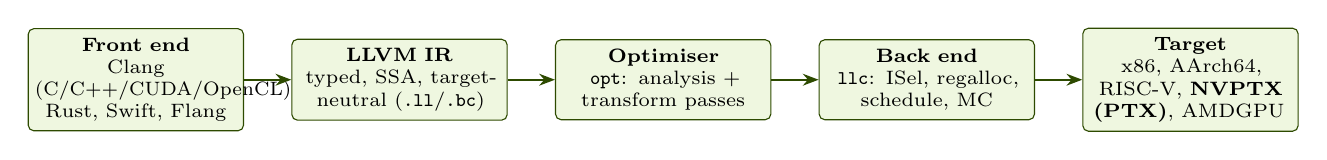
\begin{tikzpicture}[node distance=6mm,every node/.style={font=\scriptsize},
 box/.style={draw=nvdark,fill=nvgreen!12,rounded corners=2pt,minimum height=8mm,align=center,text width=2.5cm},
 arr/.style={-{Stealth[length=2mm]},thick,nvdark}]
\node[box] (fe) {\textbf{Front end}\\ Clang (C/C++/CUDA/OpenCL), Rust, Swift, Flang};
\node[box,right=of fe] (ir) {\textbf{LLVM IR}\\ typed, SSA, target-neutral (\texttt{.ll}/\texttt{.bc})};
\node[box,right=of ir] (opt) {\textbf{Optimiser}\\ \texttt{opt}: analysis + transform passes};
\node[box,right=of opt] (be) {\textbf{Back end}\\ \texttt{llc}: ISel, regalloc, schedule, MC};
\node[box,right=of be] (out) {\textbf{Target}\\ x86, AArch64, RISC-V, \textbf{NVPTX (PTX)}, AMDGPU};
\foreach \a/\b in {fe/ir,ir/opt,opt/be,be/out} \draw[arr] (\a)--(\b);
\end{tikzpicture}
\end{center}
\begin{center}\small
\begin{tabularx}{\textwidth}{@{}L{4.4cm}Y@{}}
\toprule
\textbf{Command} & \textbf{Purpose}\\
\midrule
\texttt{clang -S -emit-llvm f.c -o f.ll} & C to textual IR (\texttt{-c -emit-llvm} for bitcode \texttt{.bc})\\
\texttt{opt -passes=mem2reg,instcombine -S f.ll} & run chosen passes; \texttt{-passes='default<O2>'} is the whole \texttt{-O2} pipeline\\
\texttt{llc -O2 -march=nvptx64 -mcpu=sm\_80 f.ll} & IR to target assembly (PTX here); \texttt{-mtriple=}, \texttt{-mattr=}\\
\texttt{lli}, \texttt{llvm-as}, \texttt{llvm-dis}, \texttt{llvm-link}, \texttt{llvm-extract} & interpret/JIT; text$\leftrightarrow$bitcode; link modules; pull out functions\\
\texttt{llvm-reduce}, \texttt{bugpoint}, \texttt{llvm-stress} & shrink a failing IR file; legacy reducer; random IR generator (Chapter~\ref{ch:verif})\\
\texttt{FileCheck}, \texttt{lit}, \texttt{not}, \texttt{count} & the test infrastructure (next chapter)\\
\texttt{llvm-mca}, \texttt{llvm-objdump}, \texttt{llvm-nm} & throughput analysis, disassembly, symbols\\
\bottomrule
\end{tabularx}
\end{center}
\textbf{Why three-phase?} Each language compiles once to IR; every optimisation is written once on IR; every new CPU/GPU needs only a back end (the $M+N$ argument of Chapter~\ref{ch:front}). The same IR below was lowered by four back ends:
\needspace{5\baselineskip}
\begin{lstlisting}[language={LLVMIR},title={f.ll: x*9 + 1}]
define i32 @f(i32 %x) {
  %m = mul i32 %x, 9
  %a = add i32 %m, 1
  ret i32 %a
}
\end{lstlisting}
\begin{lstlisting}[style=shcmd]
$ llc -O2 -march=<target> f.ll   # x86-64, aarch64, riscv64, nvptx64
\end{lstlisting}
\begin{lstlisting}[style=out]
--- x86-64
    lea    eax, [rdi + 8*rdi + 1]
    ret
--- aarch64
    add    w8, w0, w0, lsl #3
    add    w0, w8, #1
    ret
--- riscv64
    slli    a1, a0, 3
    add    a0, a1, a0
    addiw    a0, a0, 1
    ret
--- nvptx64
    ld.param.u32     %r1, [f_param_0];
    mad.lo.s32     %r2, %r1, 9, 1;
    st.param.b32     [func_retval0+0], %r2;
    ret;
\end{lstlisting}
\textbf{Observe:} x86 does it with one \texttt{lea} (address arithmetic computes $x+8x+1$); AArch64 uses a shifted-operand add; RISC-V has no such fused form, so three instructions; NVPTX emits a PTX multiply-add \texttt{mad.lo.s32} with the constants as immediates. One IR, four instruction selectors: this is why a verification team runs the \emph{same test} against many targets (including the Arm and RISC-V embedded ones).

\section{IR in one page \prio{3}}
\begin{mustbox}[Reading LLVM IR]
\begin{itemize}[nosep]
\item A \textbf{module} has globals and \textbf{functions}; a function has \textbf{basic blocks} (labels), each ending in exactly one \emph{terminator} (\texttt{br}, \texttt{ret}, \texttt{switch}, \texttt{unreachable}). Every instruction producing a value defines a \textbf{virtual register} \texttt{\%name} exactly once (\textbf{SSA}). Unnamed values are numbered \texttt{\%0, \%1, \textbackslash{}ldots} in order.
\item \textbf{Types:} \texttt{i1 i8 i32 i64} (any width), \texttt{float double half bfloat}, \texttt{ptr} (a single \emph{opaque} pointer type since LLVM 15: the pointee type lives on the \emph{access}, not the pointer), vectors \texttt{<4 x i32>}, arrays \texttt{[8 x i32]}, structs \texttt{\{i32, double\}}.
\item \textbf{Instructions:} arithmetic (\texttt{add sub mul sdiv udiv srem shl lshr ashr and or xor}, \texttt{fadd fmul \textbackslash{}ldots}); comparison \texttt{icmp slt/ult/eq\textbackslash{}ldots} (signed vs.\ unsigned is in the \emph{predicate}, not the type) and \texttt{fcmp}; memory \texttt{alloca load store getelementptr}; control \texttt{br phi select call}; casts \texttt{trunc zext sext bitcast ptrtoint fptosi sitofp}; atomics \texttt{atomicrmw cmpxchg fence}.
\item \textbf{Flags and attributes} carry facts for the optimiser: \texttt{nsw}/\texttt{nuw} (no signed/unsigned wrap), \texttt{inbounds}, \texttt{fast}/\texttt{nnan}/\texttt{contract} (floating-point), \texttt{noalias}, \texttt{readonly}, \texttt{nounwind}, \texttt{align N}; \textbf{metadata} (\texttt{!tbaa}, \texttt{!llvm.loop}, debug info) is advisory and may be dropped.
\end{itemize}
\end{mustbox}

\subsection{From C to optimised IR: the full story on one function}
\begin{lstlisting}[language={C}]
int sum_to(int n) { int s = 0; for (int i = 0; i < n; i++) s += i; return s; }
\end{lstlisting}
\textbf{Step 1: Clang at \texttt{-O0}.} The front end is simple-minded: every local variable becomes a stack slot (\texttt{alloca}) with explicit \texttt{load}/\texttt{store}; \texttt{nsw} records that signed overflow is undefined in C.
\begin{lstlisting}[style=shcmd]
$ clang -O0 -Xclang -disable-O0-optnone -S -emit-llvm sum.c -o sum0.ll
\end{lstlisting}
\begin{lstlisting}[language={LLVMIR},style=out]
define dso_local i32 @sum_to(i32 noundef %0) {
  %2 = alloca i32, align 4
  %3 = alloca i32, align 4
  %4 = alloca i32, align 4
  store i32 %0, ptr %2, align 4
  store i32 0, ptr %3, align 4
  store i32 0, ptr %4, align 4
  br label %5
5:                                                ; preds = %13, %1
  %6 = load i32, ptr %4, align 4
  %7 = load i32, ptr %2, align 4
  %8 = icmp slt i32 %6, %7
  br i1 %8, label %9, label %16
9:                                                ; preds = %5
  %10 = load i32, ptr %4, align 4
  %11 = load i32, ptr %3, align 4
  %12 = add nsw i32 %11, %10
  store i32 %12, ptr %3, align 4
  br label %13
13:                                               ; preds = %9
  %14 = load i32, ptr %4, align 4
  %15 = add nsw i32 %14, 1
  store i32 %15, ptr %4, align 4
  br label %5, !llvm.loop !6
16:                                               ; preds = %5
  %17 = load i32, ptr %3, align 4
  ret i32 %17
}
\end{lstlisting}
\textbf{Step 2: \texttt{mem2reg}} promotes the stack slots to SSA values. This is exactly the dominance-frontier algorithm of Chapter~\ref{ch:sem}: the loop header gets one $\varphi$ per loop-carried variable (\texttt{\%.01} is \texttt{s}, \texttt{\%.0} is \texttt{i}).
\begin{lstlisting}[style=shcmd]
$ opt -passes=mem2reg -S sum0.ll
\end{lstlisting}
\begin{lstlisting}[language={LLVMIR},style=out]
define dso_local i32 @sum_to(i32 noundef %0) {
  br label %2
2:                                                ; preds = %6, %1
  %.01 = phi i32 [ 0, %1 ], [ %5, %6 ]
  %.0 = phi i32 [ 0, %1 ], [ %7, %6 ]
  %3 = icmp slt i32 %.0, %0
  br i1 %3, label %4, label %8
4:                                                ; preds = %2
  %5 = add nsw i32 %.01, %.0
  br label %6
6:                                                ; preds = %4
  %7 = add nsw i32 %.0, 1
  br label %2, !llvm.loop !6
8:                                                ; preds = %2
  ret i32 %.01
}
\end{lstlisting}
\textbf{Step 3: the full \texttt{-O2} pipeline.} Scalar-evolution analysis recognises that \texttt{s} is the sum of an arithmetic progression and replaces the \emph{entire loop} by the closed form $n(n-1)/2$ (computed in 33-bit arithmetic so that the intermediate product cannot overflow), then \texttt{loop-deletion} removes the loop. A guard keeps the result 0 for $n\le0$.
\begin{lstlisting}[style=shcmd]
$ clang -O2 -S -emit-llvm sum.c -o -
\end{lstlisting}
\begin{lstlisting}[language={LLVMIR},style=out]
define dso_local i32 @sum_to(i32 noundef %0) local_unnamed_addr {
  %2 = icmp sgt i32 %0, 0
  br i1 %2, label %3, label %13
3:                                                ; preds = %1
  %4 = add nsw i32 %0, -1
  %5 = zext nneg i32 %4 to i33
  %6 = add nsw i32 %0, -2
  %7 = zext i32 %6 to i33
  %8 = mul i33 %5, %7
  %9 = lshr i33 %8, 1
  %10 = trunc i33 %9 to i32
  %11 = add i32 %10, %0
  %12 = add i32 %11, -1
  br label %13
13:                                               ; preds = %3, %1
  %14 = phi i32 [ 0, %1 ], [ %12, %3 ]
  ret i32 %14
}
\end{lstlisting}
\begin{tipbox}[What this one example teaches]
(1) Front ends emit naive IR and rely on the optimiser. (2) \texttt{mem2reg}/\texttt{sroa} is the gateway pass: nothing else works well on memory. (3) The optimiser reasons \emph{algebraically} (induction variables, closed forms), not just locally. (4) It can only do this because signed overflow is undefined (\texttt{nsw}): with unsigned or wrapping arithmetic the transformation would need extra care.
\end{tipbox}

\section{Memory addressing, flags, poison \prio{3}}
\subsection{\texttt{getelementptr} (GEP) and \texttt{inbounds} (asked in S10)}
\begin{mustbox}
\texttt{getelementptr} only \textbf{computes an address}: it never reads or writes memory. Form: \texttt{getelementptr <type>, ptr <base>, <idx0>, <idx1>, \textbackslash{}ldots} where the first index steps over whole \emph{objects of the source type} (\texttt{base + idx0 * sizeof(type)}) and later indices select into aggregates (struct field numbers must be constants). \texttt{inbounds} promises that the base and the result both point within (or one past) the same allocated object; if violated the result is \textbf{poison}. That promise lets the optimiser assume non-overlap and reorder accesses.
\end{mustbox}
\begin{lstlisting}[language={C}]
struct S { int a; double b; char c; };
int    get_idx(int *p, long i)           { return p[i]; }
double get_b(struct S *s)                { return s->b; }
int    get_2d(int m[4][8], int i, int j) { return m[i][j]; }
int    add_s(int x)                      { return x + 1; }
unsigned add_u(unsigned x)               { return x + 1; }
int    mul8(int x)                       { return x * 8; }
\end{lstlisting}
\begin{lstlisting}[style=shcmd]
$ clang -O1 -S -emit-llvm gep.c -o -   (metadata and attributes trimmed)
\end{lstlisting}
\begin{lstlisting}[language={LLVMIR},style=out]
%struct.S = type { i32, double, i8 }
define i32 @get_idx(ptr nocapture readonly %0, i64 %1) {
  %3 = getelementptr inbounds i32, ptr %0, i64 %1
  %4 = load i32, ptr %3, align 4
  ret i32 %4
}
define double @get_b(ptr nocapture readonly %0) {
  %2 = getelementptr inbounds %struct.S, ptr %0, i64 0, i32 1
  %3 = load double, ptr %2, align 8
  ret double %3
}
define i32 @get_2d(ptr nocapture readonly %0, i32 %1, i32 %2) {
  %4 = sext i32 %1 to i64
  %5 = sext i32 %2 to i64
  %6 = getelementptr inbounds [8 x i32], ptr %0, i64 %4, i64 %5
  %7 = load i32, ptr %6, align 4
  ret i32 %7
}
define i32 @add_s(i32 %0) {
  %2 = add nsw i32 %0, 1
  ret i32 %2
}
define i32 @add_u(i32 %0) {
  %2 = add i32 %0, 1
  ret i32 %2
}
define i32 @mul8(i32 %0) {
  %2 = shl nsw i32 %0, 3
  ret i32 %2
}
\end{lstlisting}
\textbf{Reading it:} \texttt{p[i]} $\to$ \texttt{getelementptr inbounds i32, ptr \%0, i64 \%1} (scaled by 4); \texttt{s->b} $\to$ field index 1 of \texttt{\%struct.S} (the byte offset, 8, comes from the data layout, not from the IR); the 2-D access indexes \texttt{[8 x i32]} rows then columns (the row stride is part of the \emph{type}, which is why the array parameter must carry its inner dimension). \textbf{Signed} \texttt{x+1} becomes \texttt{add nsw}, \textbf{unsigned} \texttt{x+1} plain \texttt{add} (wraps by definition): the signedness of C arithmetic is encoded as flags, and \texttt{x*8} became \texttt{shl nsw 3}.
\subsection{Poison, undef, freeze, and why miscompilations happen}
\begin{defbox}[Deferred undefined behaviour]
\textbf{\texttt{poison}}: the result of an instruction whose assumption was violated (\texttt{nsw} overflow, out-of-bounds \texttt{inbounds} GEP, out-of-range shift, \texttt{nnan} producing NaN). Any instruction using poison yields poison; using it in a branch condition or as an address, or storing it to externally visible memory, is \emph{real} undefined behaviour. \textbf{\texttt{undef}}: an arbitrary but \emph{unspecified} value that may differ at each use (being phased out). \textbf{\texttt{freeze}}: converts poison/undef to some \emph{fixed} arbitrary value, stopping propagation.
\end{defbox}
Most real LLVM miscompilations are \emph{refinement errors}: a pass assumes a flag it may not (e.g.\ keeps \texttt{nsw} when it widened an operation, or moves a \texttt{select}'s operand out of its guard so poison leaks). The tool for catching these is \textbf{translation validation}: \emph{Alive2} checks, with an SMT solver, that the optimised function \emph{refines} the original for all inputs (it found 47 new LLVM bugs when run over the existing test-suite, PLDI 2021). Chapter~\ref{ch:verif} returns to this.

\section{The pass manager and the passes you should recognise \prio{3}}
\begin{mustbox}
LLVM has \textbf{analysis passes} (compute information: \texttt{domtree}, \texttt{loops}, \texttt{scalar-evolution}, alias analysis, \texttt{memoryssa}, block frequency) and \textbf{transform passes}. The \emph{new pass manager} (\texttt{opt -passes=}) runs a pipeline on modules/functions/loops, caches analyses, and \textbf{invalidates} an analysis unless the transform declares it preserved: forgetting to preserve or invalidate correctly is a classic bug class. Passes run in a deliberate order (cleanup after inlining, loop passes before the vectoriser).
\end{mustbox}
\begin{center}\small
\begin{tabularx}{\textwidth}{@{}L{3.2cm}Y@{}}
\toprule
\textbf{Pass} & \textbf{What it does}\\
\midrule
\texttt{sroa}, \texttt{mem2reg} & break up/promote \texttt{alloca}s to SSA values (the gateway)\\
\texttt{instcombine} & peephole algebra and canonicalisation on IR (\texttt{mul x,8} $\to$ \texttt{shl x,3}, \texttt{x+0} $\to$ \texttt{x}); the largest pass; frequent bug site\\
\texttt{simplifycfg} & merge/remove blocks, fold constant branches, turn small \texttt{if}s into \texttt{select}\\
\texttt{early-cse}, \texttt{gvn} & redundancy elimination: value numbering, redundant-load elimination (uses alias analysis, MemorySSA)\\
\texttt{licm} & hoist loop-invariant code, sink stores\\
\texttt{loop-rotate}, \texttt{indvars}, \texttt{loop-deletion}, \texttt{loop-idiom} & canonical loop shape; induction-variable simplification using scalar evolution; delete dead loops; recognise \texttt{memset}/\texttt{memcpy} loops\\
\texttt{loop-unroll}, \texttt{loop-vectorize}, \texttt{slp-vectorizer} & unroll; vectorise loops; vectorise straight-line code\\
\texttt{inline}, \texttt{ipsccp}, \texttt{deadargelim}, \texttt{globalopt} & interprocedural: inlining, constant propagation across calls, dead-argument removal, global-variable optimisation\\
\texttt{jump-threading}, \texttt{reassociate}, \texttt{adce}, \texttt{tailcallelim} & thread branches through known conditions, canonicalise operand order, aggressive DCE, tail recursion\\
\bottomrule
\end{tabularx}
\end{center}
\textbf{Debugging a miscompile with the pass manager.} \texttt{-opt-bisect-limit=N} runs only the first $N$ pass-invocations. Binary-search $N$ to find the single pass invocation that turns a good program into a bad one: the standard first step of triage (the \texttt{git bisect} of optimisation passes).
\begin{lstlisting}[style=shcmd]
$ clang -O2 -Xclang -disable-llvm-passes -S -emit-llvm sum.c -o sum_raw.ll && opt -passes='default<O2>' -opt-bisect-limit=6 -S sum_raw.ll -o /dev/null
\end{lstlisting}
\begin{lstlisting}[style=out]
BISECT: running pass (1) Annotation2MetadataPass on [module]
BISECT: running pass (2) ForceFunctionAttrsPass on [module]
BISECT: running pass (3) InferFunctionAttrsPass on [module]
BISECT: running pass (4) LowerExpectIntrinsicPass on sum_to
BISECT: running pass (5) SimplifyCFGPass on sum_to
BISECT: running pass (6) SROAPass on sum_to
BISECT: NOT running pass (7) EarlyCSEPass on sum_to
BISECT: NOT running pass (8) OpenMPOptPass on [module]
BISECT: NOT running pass (9) IPSCCPPass on [module]
\end{lstlisting}
Other instruments: \texttt{-debug-pass-manager} (which passes run), \texttt{-print-after-all} / \texttt{-print-changed} (IR after each pass), \texttt{-Rpass=\textbackslash{}ldots}, \texttt{-Rpass-missed=\textbackslash{}ldots}, \texttt{-Rpass-analysis=\textbackslash{}ldots} (optimisation remarks, e.g.\ the inliner's cost/threshold decisions below), \texttt{-mllvm -debug-only=\textbackslash{}ldots} (pass internals, debug builds).
\begin{lstlisting}[language={C}]
static int square(int x) { return x * x; }
int big(int x) { int s = 0; for (int i = 0; i < 100; i++) s += (x * i) ^ (s >> 3) + i * i + 12345 * x; return s; }
int use(int a) { return square(a) + big(a); }
\end{lstlisting}
\begin{lstlisting}[style=shcmd]
$ clang -O2 -c inl.c -Rpass=inline
\end{lstlisting}
\begin{lstlisting}[style=out]
line 3: remark: 'square' inlined into 'use' with (cost=-15030, threshold=337) at callsite use:0:25; [-Rpass=inline]
line 3: remark: 'big' inlined into 'use' with (cost=20, threshold=225) at callsite use:0:37; [-Rpass=inline]
\end{lstlisting}
\textbf{Reading it:} the inliner computes a \emph{cost} for each call site and inlines when it is below a \emph{threshold}: \texttt{square} has hugely negative cost (inlining makes it vanish into a multiply), \texttt{big} was inlined because its single call site made the copy free. This is the ``benefit versus cost'' pattern interviewers want.

\section{Vectorisation in IR \prio{2}}
\begin{lstlisting}[language={C}]
void add_arrays(int *restrict a, const int *restrict b, const int *restrict c, int n) { for (int i = 0; i < n; i++) a[i] = b[i] + c[i]; }
\end{lstlisting}
\begin{lstlisting}[style=shcmd]
$ clang -O2 -S -emit-llvm vec2.c -o - | grep '<4 x i32>'
\end{lstlisting}
\begin{lstlisting}[language={LLVMIR},style=out]
%15 = load <4 x i32>, ptr %13, align 4
%16 = load <4 x i32>, ptr %14, align 4
%19 = load <4 x i32>, ptr %17, align 4
%20 = load <4 x i32>, ptr %18, align 4
%21 = add nsw <4 x i32> %19, %15
%22 = add nsw <4 x i32> %20, %16
store <4 x i32> %21, ptr %23, align 4
store <4 x i32> %22, ptr %24, align 4
\end{lstlisting}
\textbf{Reading it:} the loop body now moves \texttt{<4 x i32>} vectors (SSE: 128 bits $=$ 4 ints), interleaved by 2 (two vectors per iteration to hide latency), with scalar remainder loops for the leftover iterations. \texttt{restrict} removed the need for a run-time overlap check. On a GPU the analogue of this SIMD loop is \emph{the thread grid itself}: each thread computes one \texttt{a[i]}.

\section{The back end: from IR to machine code \prio{2}}
\begin{enumerate}[nosep]
\item \textbf{Instruction selection} turns IR into target \emph{MachineInstrs} with virtual registers, using patterns written in TableGen (\texttt{.td}) files. Two implementations: \textbf{SelectionDAG} (per-basic-block DAG: build, legalise types/operations, combine, select, schedule) and the newer \textbf{GlobalISel} (IRTranslator, Legalizer, RegBankSelect, InstructionSelect).
\item \textbf{Register allocation} (greedy allocator with live-range splitting by default; fast allocator at \texttt{-O0}) maps virtual to physical registers and inserts spills. \textbf{Scheduling}, prologue/epilogue insertion, branch relaxation, peepholes follow, then the \textbf{MC layer} emits assembly or an object file.
\end{enumerate}
\begin{lstlisting}[style=shcmd]
$ llc -O2 -march=x86-64 -stop-after=finalize-isel f.ll -o - | sed -n '/bb.0/,/RET/p'
\end{lstlisting}
\begin{lstlisting}[style=out]
  bb.0 (%ir-block.0):
    liveins: $edi
  
    %0:gr32 = COPY $edi
    %2:gr64 = IMPLICIT_DEF
    %1:gr64_nosp = INSERT_SUBREG %2, %0, %subreg.sub_32bit
    %3:gr32 = LEA64_32r %1, 8, %1, 1, $noreg
    $eax = COPY %3
    RET 0, $eax
\end{lstlisting}
This is \textbf{MachineIR (MIR)} right after instruction selection: virtual registers (\texttt{\%0:gr32}) with register \emph{classes}, and the \texttt{LEA64\_32r} pattern already chosen. \texttt{-stop-after=<pass>} and \texttt{-run-pass=<pass>} let you run a back-end pass in isolation on an MIR file: the same trick used for back-end regression tests.

\section{MLIR, Triton and the AI-compiler ecosystem \prio{2}}
\begin{itemize}[nosep]
\item \textbf{MLIR} (Multi-Level IR, part of the LLVM project) generalises LLVM IR into \emph{dialects} of operations (each with types, attributes and \emph{regions}), so a compiler can keep high-level structure (tensors, loops, GPU kernels) and \emph{progressively lower}: e.g.\ \texttt{linalg} $\to$ \texttt{scf}/\texttt{affine} loops $\to$ \texttt{gpu} $\to$ \texttt{nvvm} $\to$ \texttt{llvm} dialect $\to$ LLVM IR $\to$ PTX. NVIDIA job postings for ``LLVM and MLIR compiler engineer'' (J6) refer to this stack.
\item \textbf{Triton} (OpenAI) compiles block-level Python kernels through MLIR and LLVM to PTX; \textbf{torch.compile/TorchInductor} generates Triton or C++; \textbf{XLA/OpenXLA} (JAX/TensorFlow), \textbf{TVM}, \textbf{TensorRT} are other ML compilers (Chapter~\ref{ch:ml}).
\end{itemize}

\section{GCC in one paragraph \prio{1}}
GCC's pipeline: front ends $\to$ \textbf{GENERIC} $\to$ \textbf{GIMPLE} (three-address, SSA-capable) $\to$ \textbf{RTL} (low-level, register-transfer) $\to$ assembly. Dump intermediate forms with \texttt{-fdump-tree-all} and \texttt{-fdump-rtl-all}; plugin pass infrastructure exists; its regression suite uses \textbf{DejaGnu} (\texttt{dg-*} directives in test comments), the analogue of lit+FileCheck. Both compilers matter to a verifier: differential testing GCC against Clang is a classic bug-finding method.

\section{Practice \prio{3}}
\begin{qn}Why does Clang emit \texttt{alloca}/\texttt{load}/\texttt{store} for every local, and which pass fixes it?\end{qn}
\begin{ans}It keeps the front end trivial: it need not compute SSA or dominance. \texttt{mem2reg}/\texttt{sroa} promote allocas to SSA registers, inserting $\varphi$ nodes at dominance frontiers.\end{ans}
\begin{qn}Does \texttt{getelementptr} access memory? What does \texttt{inbounds} mean?\end{qn}
\begin{ans}No: it is pure address arithmetic. \texttt{inbounds} asserts the computed address stays within the same allocated object (or one past the end); violating it yields poison, enabling alias reasoning.\end{ans}
\begin{qn}What is the difference between \texttt{add}, \texttt{add nsw} and \texttt{add nuw}?\end{qn}
\begin{ans}Plain \texttt{add} wraps modulo $2^n$. \texttt{nsw}: signed overflow produces \emph{poison}; \texttt{nuw}: unsigned overflow produces poison. C's signed overflow is UB, so Clang emits \texttt{nsw}; unsigned C arithmetic wraps, so it emits plain \texttt{add}.\end{ans}
\begin{qn}How do you find which optimisation pass broke a program?\end{qn}
\begin{ans}Bisect: \texttt{-opt-bisect-limit=N} (or \texttt{-mllvm -opt-bisect-limit=N} from Clang) disables all pass invocations after the $N$th. Binary-search the smallest $N$ that miscompiles; the $N$-th pass invocation (printed as \texttt{BISECT: running pass (N) \textbackslash{}ldots}) is the culprit. Then reduce the IR (\texttt{llvm-reduce}) and report.\end{ans}
\begin{qn}Why can a vectoriser not vectorise \texttt{a[i] = a[i-1] + 1}, and what would let it vectorise \texttt{a[i] = b[i] + c[i]} without a run-time check?\end{qn}
\begin{ans}The first has a loop-carried flow dependence of distance 1. The second needs proof that \texttt{a} does not overlap \texttt{b} and \texttt{c}: \texttt{restrict} (or \texttt{noalias}), or the compiler emits a run-time overlap check and a scalar fallback loop.\end{ans}
\begin{qn}Name the parts of LLVM's back end and the TableGen files' role.\end{qn}
\begin{ans}Instruction selection (SelectionDAG/GlobalISel), scheduling, register allocation, prologue/epilogue, MC emission. TableGen \texttt{.td} files declaratively describe registers, instructions, and instruction-selection patterns, from which C++ tables are generated.\end{ans}


% ===== 13-filecheck.tex.in =====
\chapter{Testing Compilers the LLVM Way: lit and FileCheck}
\label{ch:filecheck}

\begin{chapbox}
\textbf{Priority \prio{2}. Time: 35 min.} The vast majority of regression tests in LLVM (tens of thousands) are tiny files with a \texttt{RUN:} line and \texttt{CHECK:} lines. A compiler-verification engineer must read and write such tests fluently; NVIDIA's own test frameworks differ, but the ideas (small inputs, exact expectations, automatic discovery, XFAIL tracking) are universal. Everything below is run for real with \texttt{lit} 23 and LLVM~18's \texttt{FileCheck}.
\end{chapbox}

\section{The test pyramid for a compiler \prio{2}}
\begin{center}\small
\begin{tabularx}{\textwidth}{@{}L{3.6cm}L{3.8cm}Y@{}}
\toprule
\textbf{Level} & \textbf{Example in LLVM} & \textbf{What it checks}\\
\midrule
Unit tests & GoogleTest C++ (\texttt{unittests/}) & APIs and data structures (APInt, pass-manager plumbing)\\
\textbf{Regression tests} & \texttt{.ll}/\texttt{.c}/\texttt{.mir} files run by \textbf{lit}, verified by \textbf{FileCheck} & the \emph{output} of one pass or tool for one tiny input: transformation happened (or did not), diagnostics, code selected\\
Execution tests & compile, run, compare output (\texttt{lli}, or build+run) & the \emph{behaviour} of generated code\\
Integration / benchmark suites & \texttt{llvm-test-suite}, SPEC CPU, application builds & large real programs: correctness and performance over time\\
Fuzzing / differential & \texttt{llvm-isel-fuzzer}, Csmith, YARPGen & bugs nobody thought to write a test for (Chapter~\ref{ch:verif})\\
\bottomrule
\end{tabularx}
\end{center}
\textbf{Rule:} every fixed compiler bug leaves behind a \emph{minimal regression test}: the reduced reproducer plus checks that fail before the fix and pass after it.

\section{lit: the test driver \prio{2}}
\begin{mustbox}
\texttt{lit} discovers test files (by suffix, configured in \texttt{lit.cfg.py}), runs the shell commands in each file's \texttt{RUN:} lines, and classifies the result:
\textbf{PASS} (all commands exit 0), \textbf{FAIL}, \textbf{XFAIL} (expected failure, declared with \texttt{XFAIL:}), \textbf{XPASS} (an XFAIL test that now passes: reported as an error so stale expectations get removed), \textbf{UNSUPPORTED} (\texttt{UNSUPPORTED:} or an unmet \texttt{REQUIRES:}), \textbf{UNRESOLVED}, \textbf{TIMEOUT}.
\end{mustbox}
\begin{center}\small
\begin{tabularx}{\textwidth}{@{}L{3.4cm}Y@{}}
\toprule
\textbf{Feature} & \textbf{Meaning}\\
\midrule
\texttt{RUN: cmd | FileCheck \%s} & a command line; the test fails if any command in the chain fails (pipelines fail if \emph{any} stage fails)\\
\texttt{\%s}, \texttt{\%S}, \texttt{\%t}, \texttt{\%p} & the test file path; its directory; a unique temp file; the same as \texttt{\%S}. Typical: \texttt{clang -S -emit-llvm \%s -o \%t.ll}\\
\texttt{REQUIRES: nvptx-registered-target} & run only if the feature exists (targets built, OS, assertions-enabled build \ldots)\\
\texttt{UNSUPPORTED: system-windows}, \texttt{XFAIL: *} & skip on a configuration; mark as a known failure\\
\texttt{not cmd}, \texttt{not --crash cmd}, \texttt{count N cmd} & invert the exit status (expect failure); expect a crash; require exactly $N$ lines of output\\
\texttt{lit -v}, \texttt{-a}, \texttt{-j N}, \texttt{--filter=RE}, \texttt{--timeout=S}, \texttt{--shard=I/N}, \texttt{--xunit-xml-output=f.xml} & show failures, show all commands, parallelism, select tests, time limit, split across CI machines, JUnit-style report for dashboards\\
\bottomrule
\end{tabularx}
\end{center}

\section{FileCheck: match the output, not the accident \prio{2}}
\begin{center}\small
\begin{tabularx}{\textwidth}{@{}L{4.3cm}Y@{}}
\toprule
\textbf{Directive} & \textbf{Semantics}\\
\midrule
\texttt{CHECK: text} & find \emph{text} somewhere after the previous match (substring match; patterns are matched in order)\\
\texttt{CHECK-NEXT:} / \texttt{CHECK-SAME:} & must be on the \emph{next} line / on the \emph{same} line as the previous match\\
\texttt{CHECK-NOT:} & text must \emph{not} appear between the surrounding matches (use to prove an instruction disappeared)\\
\texttt{CHECK-LABEL:} & anchors a function or section; the other checks are matched \emph{within} it, so one failing function does not confuse the next\\
\texttt{CHECK-DAG:} & a group of lines that may appear in \emph{any} order (e.g.\ independent loads)\\
\texttt{CHECK-COUNT-N:}, \texttt{CHECK-EMPTY:} & exactly $N$ consecutive matches; an empty line\\
\texttt{\{\{regex\}\}} & inline regular expression: \texttt{add i32 \{\{\%[0-9]+\}\}, 1}\\
\texttt{[[NAME:regex]]}, \texttt{[[NAME]]} & \textbf{capture} a value then require it again: \texttt{[[R:\%.*]] = shl i32 \%x, 3 \textbackslash{}ldots ret i32 [[R]]}. Numeric variants \texttt{[[\#N:]]}, \texttt{[[\#N+1]]}\\
\texttt{--check-prefix=P}, \texttt{--implicit-check-not=T} & several expectation sets in one file (e.g.\ per optimisation level); forbid \texttt{T} everywhere\\
\texttt{--dump-input=fail}, \texttt{--strict-whitespace}, \texttt{--match-full-lines}, \texttt{-DVAR=value} & show the annotated input on failure; whitespace-exact; whole-line matches; pass substitutions from \texttt{RUN:}\\
\bottomrule
\end{tabularx}
\end{center}

\subsection{A real mini test suite}
Four tests for the \texttt{instcombine} pass: the first two pass, one is an expected failure (a known bug) and one is \emph{wrong on purpose} so you can see how FileCheck explains a failure.
\needspace{5\baselineskip}
\begin{lstlisting}[language={LLVMIR},title={tests/mul8.ll}]
; RUN: opt -passes=instcombine -S %s | FileCheck %s

define i32 @mul8(i32 %x) {
  %r = mul i32 %x, 8
  ret i32 %r
}
; CHECK-LABEL: define i32 @mul8(
; CHECK-NEXT:    [[R:%.*]] = shl i32 %x, 3
; CHECK-NEXT:    ret i32 [[R]]
\end{lstlisting}
\needspace{5\baselineskip}
\begin{lstlisting}[language={LLVMIR},title={tests/identity.ll}]
; RUN: opt -passes=instcombine -S %s | FileCheck %s
; Algebraic identities must disappear entirely.

define i32 @ident(i32 %x) {
  %a = add i32 %x, 0
  %b = mul i32 %a, 1
  %c = xor i32 %b, 0
  ret i32 %c
}
; CHECK-LABEL: @ident(
; CHECK-NOT:     add
; CHECK-NOT:     mul
; CHECK-NOT:     xor
; CHECK:         ret i32 %x
\end{lstlisting}
\needspace{5\baselineskip}
\begin{lstlisting}[language={LLVMIR},title={tests/xfail\_example.ll}]
; RUN: opt -passes=instcombine -S %s | FileCheck %s
; XFAIL: *
; Known missed optimisation, tracked elsewhere: XFAIL keeps the suite green until it is fixed.

define i32 @f(i32 %x) {
  %r = mul i32 %x, 3
  ret i32 %r
}
; CHECK: shl i32 %x, 2
\end{lstlisting}
\needspace{5\baselineskip}
\begin{lstlisting}[language={LLVMIR},title={tests/wrong\_expectation.ll (wrong on purpose)}]
; RUN: opt -passes=instcombine -S %s | FileCheck %s

define i32 @f(i32 %x) {
  %r = mul i32 %x, 8
  ret i32 %r
}
; CHECK-LABEL: @f(
; CHECK: mul i32 %x, 8
\end{lstlisting}
\needspace{5\baselineskip}
\begin{lstlisting}[language={Python},title={lit.cfg.py}]
import os, lit.formats
config.name = "mini-llvm-tests"
config.test_format = lit.formats.ShTest(execute_external=False)      # lit's built-in shell: pipes and redirects work everywhere
config.suffixes = [".ll"]
config.test_source_root = os.path.dirname(__file__)
config.environment["PATH"] = os.pathsep.join(["/usr/lib/llvm-18/bin", config.environment["PATH"]])   # find opt and FileCheck
\end{lstlisting}
\begin{lstlisting}[style=shcmd]
$ lit -v -j1 tests
\end{lstlisting}
\begin{lstlisting}[style=out]
-- Testing: 4 tests, 1 workers --
FAIL: mini-llvm-tests :: tests/wrong_expectation.ll (1 of 4)
******************** TEST 'mini-llvm-tests :: tests/wrong_expectation.ll' FAILED ********************
Exit Code: 1

Command Output (stdout):
--
# RUN: at line 1
opt -passes=instcombine -S tests/wrong_expectation.ll | FileCheck tests/wrong_expectation.ll
# executed command: opt -passes=instcombine -S tests/wrong_expectation.ll
# executed command: FileCheck tests/wrong_expectation.ll
# .---command stderr------------
# | tests/wrong_expectation.ll:8:10: error: CHECK: expected string not found in input
# | ; CHECK: mul i32 %x, 8
# |          ^
# | <stdin>:4:15: note: scanning from here
# | define i32 @f(i32 %x) {
# |               ^
# | <stdin>:5:7: note: possible intended match here
# |  %r = shl i32 %x, 3
# |       ^
# | 
# | Input file: <stdin>
# | Check file: tests/wrong_expectation.ll
# | 
# | -dump-input=help explains the following input dump.
# | 
# | Input was:
# | <<<<<<
# |            1: ; ModuleID = 'tests/wrong_expectation.ll' 
# |            2: source_filename = "tests/wrong_expectation.ll" 
# |            3:  
# |            4: define i32 @f(i32 %x) { 
# | check:8'0                   X~~~~~~~~~ error: no match found
# |            5:  %r = shl i32 %x, 3 
# | check:8'0     ~~~~~~~~~~~~~~~~~~~~
# | check:8'1           ?              possible intended match
# |            6:  ret i32 %r 
# | check:8'0     ~~~~~~~~~~~~
# |            7: } 
# | check:8'0     ~~
# | >>>>>>
# `-----------------------------
# error: command failed with exit status: 1

--

********************
PASS: mini-llvm-tests :: tests/identity.ll (2 of 4)
PASS: mini-llvm-tests :: tests/mul8.ll (3 of 4)
XFAIL: mini-llvm-tests :: tests/xfail_example.ll (4 of 4)
********************
Failed Tests (1):
  mini-llvm-tests :: tests/wrong_expectation.ll



Total Discovered Tests: 4
  Passed           : 2 (50.00%)
  Expectedly Failed: 1 (25.00%)
  Failed           : 1 (25.00%)
\end{lstlisting}
\begin{exbox}[Reading lit's report]
\begin{itemize}[nosep]
\item \textbf{PASS} for the first two; \textbf{XFAIL} for the known-bug test (counted as success; if the bug were fixed it would show \textbf{XPASS} and fail the run, forcing the \texttt{XFAIL} line to be deleted).
\item FileCheck's failure message is the model of a good diagnostic: the \emph{exact check line}, where it scanned from, and a \emph{possible intended match} (\texttt{\%r = shl i32 \%x, 3}): the optimiser did \emph{better} than the test expected (strength reduction), so here the test, not the compiler, is wrong.
\item \texttt{CHECK-NOT} in \texttt{identity.ll} proves the three no-op instructions were removed; \texttt{[[R:\%.*]]} captured the register name so the test does not depend on how values happen to be numbered.
\end{itemize}
\end{exbox}

\section{Writing tests that survive refactoring \prio{2}}
\begin{mustbox}
\begin{itemize}[nosep]
\item \textbf{Minimal and focused:} one behaviour per test; reduce with \texttt{llvm-reduce}/\texttt{creduce} before committing. A 3-line test is read; a 300-line test is ignored.
\item \textbf{Check intent, not accident:} capture registers with \texttt{[[VAR:\%.*]]}, use \texttt{CHECK-DAG} where order is unspecified, \texttt{CHECK-LABEL} per function, and avoid pinning unrelated instructions or exact scheduling unless that is what is under test.
\item \textbf{Generated checks:} LLVM's \texttt{utils/update\_test\_checks.py} (IR) and \texttt{update\_llc\_test\_checks.py} (assembly) write \texttt{CHECK} lines from current output. Fast, but they \emph{bless whatever the compiler does today}: always review the diff for semantic sense.
\item \textbf{Target selection:} pin \texttt{-mtriple=nvptx64-nvidia-cuda -mcpu=sm\_80}; guard with \texttt{REQUIRES: nvptx-registered-target}; keep target-independent tests target-independent.
\item \textbf{Negative tests:} \texttt{not opt \textbackslash{}ldots} for invalid input that must be rejected; Clang's \texttt{-verify} with \texttt{// expected-error \{\{message\}\}} comments for diagnostics; \texttt{not --crash} documents a currently-crashing input.
\item \textbf{Execution tests} compile and \emph{run}: compare output or exit status; keep them deterministic (Chapter~\ref{ch:verif}). Separate \emph{performance} tests from correctness tests; performance needs statistics, not CHECK lines.
\end{itemize}
\end{mustbox}
For NVIDIA-style work the analogue is a tiny \emph{PTX} or \emph{CUDA} file, a \texttt{RUN:} that assembles/compiles it for a target, and checks on either the generated \emph{code} (a given PTX instruction becomes the expected SASS) or the executed \emph{result} on a GPU or simulator. Chapter~\ref{ch:lab} implements a Python mini-FileCheck and test runner you can describe in an interview.

\section{Practice \prio{2}}
\begin{qn}Which directive proves that an optimisation removed an instruction, and where must it be placed?\end{qn}
\begin{ans}\texttt{CHECK-NOT: <text>}. It applies between the matches that surround it (so put it between two positive checks, or after \texttt{CHECK-LABEL}), or use \texttt{--implicit-check-not}. It must be bracketed by positive checks or it will search to the end of the input.\end{ans}
\begin{qn}Why is hard-coding \texttt{\%3 = add i32 \textbackslash{}ldots} in a check line fragile, and what replaces it?\end{qn}
\begin{ans}Value numbering changes when unrelated instructions change. Capture with \texttt{[[V:\%.*]] = add i32 \textbackslash{}ldots} and reuse \texttt{[[V]]}.\end{ans}
\begin{qn}What does \textbf{XPASS} mean and why does lit treat it as a failure?\end{qn}
\begin{ans}A test marked \texttt{XFAIL} passed: the bug it tracked was fixed (or the test changed). Failing the run forces maintainers to delete the stale \texttt{XFAIL}, keeping the expectation file honest.\end{ans}
\begin{qn}You are asked to add a test for a miscompilation. List what the test directory should contain.\end{qn}
\begin{ans}A minimal reproducer (reduced), a \texttt{RUN:} line that invokes the exact tool and flags, checks that distinguish correct from incorrect output (code pattern or runtime value), a comment linking the bug report, and \texttt{REQUIRES:} for the needed target/feature. It must fail on the unfixed compiler and pass on the fixed one.\end{ans}


% ===== 14a-ptx.tex.in =====
\chapter{NVIDIA's Stack: nvcc, NVVM, PTX and SASS}
\label{ch:ptx}

\begin{chapbox}
\textbf{Priority \prio{3} for the pipeline and PTX vocabulary, \prio{2} for details. Time: 90 min.} The role description names PTX, CUDA and GPU assembly explicitly. The sandbox has no CUDA SDK or GPU, so this chapter is grounded in what the \emph{open-source LLVM NVPTX back end} generates for real CUDA kernels (Clang's CUDA front end, no SDK needed for device-only compilation). It is the same instruction set (PTX) that NVIDIA's own \texttt{cicc}/NVVM emits; instruction \emph{choices} and register names differ from NVIDIA's closed compiler, \emph{syntax and semantics} do not. Sources: NVIDIA \src{https://docs.nvidia.com/cuda/cuda-compiler-driver-nvcc/}{nvcc documentation} and the PTX ISA manual (\src{https://docs.nvidia.com/cuda/pdf/ptx_isa_8.7.pdf}{PDF, versions up to 9.1 exist}); read PTX ISA chapters 5--9 if you have an hour spare.
\end{chapbox}



\section{The CUDA compilation pipeline \prio{3}}
\begin{center}
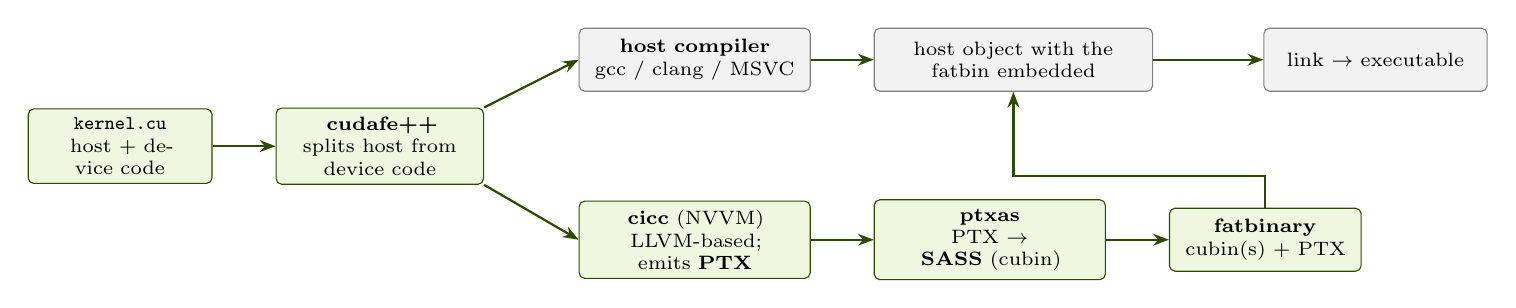
\begin{tikzpicture}[node distance=5mm and 8mm,every node/.style={font=\scriptsize},
 box/.style={draw=nvdark,fill=nvgreen!12,rounded corners=2pt,minimum height=8mm,align=center,text width=2.7cm},
 host/.style={draw=black!50,fill=black!5,rounded corners=2pt,minimum height=8mm,align=center,text width=2.7cm},
 arr/.style={-{Stealth[length=2mm]},thick,nvdark}]
\node[box,text width=2.1cm] (cu) {\texttt{kernel.cu}\\ host + device code};
\node[box,right=of cu,text width=2.4cm] (fe) {\textbf{cudafe++}\\ splits host from device code};
\node[host,above right=2mm and 12mm of fe] (hc) {\textbf{host compiler}\\ gcc / clang / MSVC};
\node[box,below right=2mm and 12mm of fe] (cicc) {\textbf{cicc} (NVVM)\\ LLVM-based; emits \textbf{PTX}};
\node[box,right=of cicc] (ptxas) {\textbf{ptxas}\\ PTX $\to$ \textbf{SASS} (cubin)};
\node[box,right=of ptxas,text width=2.2cm] (fb) {\textbf{fatbinary}\\ cubin(s) + PTX};
\node[host,right=of hc,text width=3.3cm] (obj) {host object with the fatbin embedded};
\node[host,right=14mm of obj,text width=2.6cm] (exe) {link $\to$ executable};
\draw[arr] (cu)--(fe); \draw[arr] (fe.north east)--(hc.west); \draw[arr] (fe.south east)--(cicc.west);
\draw[arr] (cicc)--(ptxas); \draw[arr] (ptxas)--(fb); \draw[arr] (hc)--(obj); \draw[arr] (obj)--(exe);
\draw[arr] (fb.north) -- ++(0,4mm) -| (obj.south);
\end{tikzpicture}
\end{center}
\begin{mustbox}
\begin{itemize}[nosep]
\item \textbf{\texttt{nvcc}} is a \emph{driver}: it separates device from host code, sends the device part through NVIDIA's compilers and assembler, embeds the result (a \textbf{fat binary}) in the host object, and forwards all ordinary C++ compilation to a host compiler. \texttt{nvcc -dryrun} prints the exact sub-commands; \texttt{--keep} keeps the intermediates (\texttt{.ptx}, \texttt{.cubin}, \texttt{.fatbin}).
\item \textbf{NVVM / \texttt{cicc}} is the LLVM-based compiler that turns the device program (in \emph{NVVM IR}, an LLVM IR dialect) into \textbf{PTX}. \textbf{\texttt{ptxas}} is the optimising assembler: PTX $\to$ architecture-specific machine code (\textbf{SASS}, in a \textbf{cubin} ELF file). Register allocation, instruction scheduling and most low-level optimisation happen in \texttt{ptxas}.
\item \textbf{Alternative front ends/APIs:} \textbf{NVRTC} compiles CUDA C++ strings to PTX/cubin at run time; \textbf{libNVVM} compiles NVVM IR; \textbf{nvJitLink} links at run time; \textbf{Clang} can compile CUDA directly (\texttt{clang++ -x cuda --cuda-gpu-arch=sm\_80}) through the open-source NVPTX back end; Triton, XLA and other compilers also emit PTX.
\item \textbf{The driver can JIT:} if a binary lacks SASS for the installed GPU it compiles the embedded \emph{PTX} at load time (result cached).
\end{itemize}
\end{mustbox}
\begin{center}\small
\begin{tabularx}{\textwidth}{@{}L{4.9cm}Y@{}}
\toprule
\textbf{nvcc option} & \textbf{Meaning}\\
\midrule
\texttt{-arch=sm\_80} & shorthand for \texttt{-gencode arch=compute\_80,code=[sm\_80,compute\_80]}: SASS for sm\_80 \emph{and} PTX for compute\_80\\
\texttt{-gencode arch=compute\_70,code=sm\_70} & virtual arch (PTX feature level) used to \emph{generate}, real arch (SASS) to \emph{emit}; repeat for a multi-architecture fat binary\\
\texttt{-ptx}, \texttt{-cubin}, \texttt{-fatbin}, \texttt{--keep} & stop at PTX / cubin / fatbin; keep intermediates\\
\texttt{-Xptxas -v}, \texttt{--maxrregcount=N}, \texttt{-lineinfo}, \texttt{-G} & report registers/shared memory/spills per kernel; cap registers per thread; line info for profilers; device debug build (disables most optimisation)\\
\texttt{--use\_fast\_math} & shorthand for \texttt{-ftz=true -prec-div=false -prec-sqrt=false --fmad=true} plus approximate intrinsics\\
\texttt{--fmad=false}, \texttt{-ftz=true} & forbid fused multiply-add contraction; flush denormals to zero\\
\texttt{-rdc=true} & relocatable device code: separate compilation of device code, then device linking\\
\bottomrule
\end{tabularx}
\end{center}
\begin{trapbox}[Virtual vs.\ real architecture (a favourite question)]
\textbf{\texttt{compute\_XY}} = virtual architecture = the PTX feature level. \textbf{\texttt{sm\_XY}} = real architecture = SASS for that hardware generation. \textbf{PTX is forward compatible:} PTX for \texttt{compute\_70} can be JIT-compiled for any GPU of compute capability $\ge$7.0. \textbf{SASS is not:} a cubin built for \texttt{sm\_XY} runs on devices of the same major version and minor $\ge Y$ (sm\_80 SASS runs on sm\_86, not the reverse, and never across major versions). So a robust library ships SASS for the architectures it was tested on \emph{plus} PTX for the newest virtual architecture. A recent generation is the Hopper family (\texttt{sm\_90}/\texttt{sm\_90a}); Blackwell adds further \texttt{sm\_100}/\texttt{sm\_120}-family targets with architecture-specific suffixes: do not memorise numbers, understand the rule.
\end{trapbox}

\section{NVVM IR: LLVM IR with GPU conventions \prio{2}}
Compile a kernel with Clang and read the IR (the stub header replaces \texttt{cuda\_runtime.h}).
\needspace{5\baselineskip}
\begin{lstlisting}[language={CUDA},title={vecadd.cu}]
#include "cuda_stub.h"
__global__ void vecadd(const float* a, const float* b, float* c, int n) {
    int i = blockIdx.x * blockDim.x + threadIdx.x;
    if (i < n) c[i] = a[i] + b[i];
}
\end{lstlisting}
\begin{lstlisting}[style=shcmd]
$ clang++ -x cuda --cuda-device-only --cuda-gpu-arch=sm_80 -O2 -S -emit-llvm vecadd.cu -o -
\end{lstlisting}
\begin{lstlisting}[language={LLVMIR},style=out]
target datalayout = "e-i64:64-i128:128-v16:16-v32:32-n16:32:64"
target triple = "nvptx64-nvidia-cuda"
define dso_local void @_Z6vecaddPKfS0_Pfi(ptr %0, ptr %1, ptr %2, i32 %3) {
  %5 = tail call i32 @llvm.nvvm.read.ptx.sreg.ctaid.x()
  %6 = tail call i32 @llvm.nvvm.read.ptx.sreg.ntid.x()
  %7 = mul i32 %5, %6
  %8 = tail call i32 @llvm.nvvm.read.ptx.sreg.tid.x()
  %9 = add i32 %7, %8
  %10 = icmp slt i32 %9, %3
  br i1 %10, label %11, label %19
11:                                               ; preds = %4
  %12 = sext i32 %9 to i64
  %13 = getelementptr inbounds float, ptr %2, i64 %12
  %14 = getelementptr inbounds float, ptr %1, i64 %12
  %15 = getelementptr inbounds float, ptr %0, i64 %12
  %16 = load float, ptr %15, align 4
  %17 = load float, ptr %14, align 4
  %18 = fadd contract float %16, %17
  store float %18, ptr %13, align 4
  br label %19
19:                                               ; preds = %11, %4
  ret void
}
declare i32 @llvm.nvvm.read.ptx.sreg.ctaid.x() #1
declare i32 @llvm.nvvm.read.ptx.sreg.ntid.x() #1
declare i32 @llvm.nvvm.read.ptx.sreg.tid.x() #1
!nvvm.annotations = !{!0}
!0 = !{ptr @_Z6vecaddPKfS0_Pfi, !"kernel", i32 1}
\end{lstlisting}
\begin{center}\small
\begin{tabularx}{\textwidth}{@{}L{3.6cm}L{5.2cm}Y@{}}
\toprule
\textbf{CUDA construct} & \textbf{NVVM IR} & \textbf{PTX}\\
\midrule
\texttt{threadIdx.x} & \texttt{call i32 @llvm.nvvm.read.ptx.sreg.tid.x()} & \texttt{mov.u32 \%r, \%tid.x;}\\
\texttt{blockIdx.x}, \texttt{blockDim.x}, \texttt{gridDim.x} & \texttt{...sreg.ctaid.x}, \texttt{...ntid.x}, \texttt{...nctaid.x} & \texttt{\%ctaid.x}, \texttt{\%ntid.x}, \texttt{\%nctaid.x}\\
\texttt{\_\_global\_\_} kernel & \texttt{!nvvm.annotations = !\{ptr @f, !"kernel", i32 1\}} (newer LLVM: \texttt{ptx\_kernel} calling convention) & \texttt{.visible .entry}\\
\texttt{\_\_shared\_\_ float s[256]} & global in \texttt{addrspace(3)} & \texttt{.shared .align 4 .b8 s[1024];}\\
\texttt{\_\_syncthreads()} & \texttt{call void @llvm.nvvm.barrier0()} & \texttt{bar.sync 0;}\\
\texttt{atomicAdd(\&x, v)} & \texttt{atomicrmw add} & \texttt{atom.global.add.u32}\\
\texttt{\_\_shfl\_down\_sync(m,v,d)} & \texttt{@llvm.nvvm.shfl.sync.down.f32} & \texttt{shfl.sync.down.b32}\\
\bottomrule
\end{tabularx}
\end{center}
\textbf{Conventions:} triple \texttt{nvptx64-nvidia-cuda}; \textbf{address spaces}: 0 generic, 1 global, 3 shared, 4 constant, 5 local; thread and block coordinates are \emph{intrinsics} reading special registers; kernels are marked by metadata. A pointer in the generic space is converted with \texttt{addrspacecast} (PTX \texttt{cvta}).

\section{PTX: the virtual ISA \prio{3}}
\begin{mustbox}[PTX in ten facts]
\begin{enumerate}[nosep]
\item PTX is a \textbf{low-level, assembly-like, text} instruction set for a \emph{virtual} GPU, documented publicly and versioned (\texttt{.version 8.x}); it is the stable target for compilers and the unit that NVIDIA's driver can JIT.
\item It has \textbf{unlimited typed virtual registers}: declared in banks like \texttt{.reg .b32 \%r<10>;} (meaning \texttt{\%r0..\%r9}); predicates are \texttt{.pred}. \texttt{ptxas} maps them to the real register file.
\item \textbf{Types:} untyped bit-size \texttt{.b8/.b16/.b32/.b64}; unsigned \texttt{.u*}; signed \texttt{.s*}; floating \texttt{.f16 .bf16 .f32 .f64} (plus packed and low-precision tensor types). Instructions state their type: \texttt{add.s32}, \texttt{add.f32}. There is no 8-bit arithmetic: bytes are loaded/stored as \texttt{.u8/.s8} and computed in 16/32 bits.
\item \textbf{Instruction format:} \texttt{[@\{!\}pred] opcode[.mod]*.type dst, src1, src2;}. Modifiers select rounding (\texttt{.rn .rz .rm .rp}), saturation (\texttt{.sat}), flush-to-zero (\texttt{.ftz}), approximation (\texttt{.approx}), width (\texttt{.lo .hi .wide}), comparison operator (\texttt{setp.lt}), cache and memory-order qualifiers.
\item \textbf{Predication:} any instruction can be guarded by a predicate register: \texttt{@\%p1 bra L;}, \texttt{@!\%p2 st.global.f32 [\%rd], \%f;}. Short conditionals become predicated or \texttt{selp} (select) code with \emph{no branch}.
\item \textbf{State spaces} name where data lives (next table); \texttt{ld/st} must say which. \texttt{cvta} converts between a space-specific and a generic address.
\item \textbf{Special registers:} \texttt{\%tid.\{x,y,z\}}, \texttt{\%ntid}, \texttt{\%ctaid}, \texttt{\%nctaid}, \texttt{\%laneid}, \texttt{\%warpid}, \texttt{\%smid}, \texttt{\%clock}, \texttt{\%globaltimer}, lane masks.
\item \textbf{Control flow:} labels and \texttt{bra}; \texttt{bra.uni} asserts that all active threads of a warp take the branch together (no divergence); \texttt{call}, \texttt{ret}, \texttt{exit}.
\item \textbf{Memory consistency:} \texttt{ld/st/atom/fence} take \emph{ordering} (\texttt{.relaxed .acquire .release .sc}) and \emph{scope} (\texttt{.cta .cluster .gpu .sys}) qualifiers; \texttt{bar.sync} is a CTA-wide barrier with memory ordering among participants.
\item \textbf{Entry points:} \texttt{.entry} = kernel (callable from the host, parameters in \texttt{.param} space); \texttt{.func} = device function. \texttt{.visible}/\texttt{.extern}/\texttt{.weak} control linkage.
\end{enumerate}
\end{mustbox}
\begin{center}\small
\begin{tabularx}{\textwidth}{@{}L{2.2cm}L{4.1cm}Y@{}}
\toprule
\textbf{State space} & \textbf{Scope / lifetime} & \textbf{CUDA analogue and notes}\\
\midrule
\texttt{.reg} & per thread & scalars/locals in registers; fastest\\
\texttt{.local} & per thread (off-chip, cached) & register spills, large per-thread arrays; \emph{slow}, despite the name\\
\texttt{.shared} & per CTA (thread block); on-chip & \texttt{\_\_shared\_\_}; banked; needs \texttt{bar.sync} to communicate\\
\texttt{.global} & all threads, host-visible & device memory (\texttt{cudaMalloc}); cached in L2 (and L1)\\
\texttt{.const} & read-only, all threads & \texttt{\_\_constant\_\_}; broadcast-friendly cache\\
\texttt{.param} & kernel/function arguments & read with \texttt{ld.param}; kernel parameters live in a constant bank\\
\bottomrule
\end{tabularx}
\end{center}

\subsection{Reading the real PTX of \texttt{vecadd}, line by line}
\begin{lstlisting}[style=shcmd]
$ clang++ -x cuda --cuda-device-only --cuda-gpu-arch=sm_80 -O2 -S vecadd.cu -o -   (comments trimmed)
\end{lstlisting}
\begin{lstlisting}[language={PTX},style=out]
.version 7.0
.target sm_80
.address_size 64
.visible .entry _Z6vecaddPKfS0_Pfi(
    .param .u64 p0,
    .param .u64 p1,
    .param .u64 p2,
    .param .u32 p3
)
{
    .reg .pred     %p<2>;
    .reg .b32     %r<6>;
    .reg .f32     %f<4>;
    .reg .b64     %rd<11>;
    ld.param.u32     %r1, [p3];
    mov.u32     %r2, %ctaid.x;
    mov.u32     %r3, %ntid.x;
    mov.u32     %r4, %tid.x;
    mad.lo.s32     %r5, %r2, %r3, %r4;
    setp.ge.s32     %p1, %r5, %r1;
    @%p1 bra     $L__BB0_2;
    ld.param.u64     %rd4, [p0];
    ld.param.u64     %rd5, [p2];
    cvta.to.global.u64     %rd6, %rd5;
    ld.param.u64     %rd7, [p1];
    cvta.to.global.u64     %rd8, %rd7;
    cvta.to.global.u64     %rd9, %rd4;
    mul.wide.s32     %rd10, %r5, 4;
    add.s64     %rd1, %rd6, %rd10;
    add.s64     %rd2, %rd8, %rd10;
    add.s64     %rd3, %rd9, %rd10;
    ld.global.f32     %f1, [%rd3];
    ld.global.f32     %f2, [%rd2];
    add.f32     %f3, %f1, %f2;
    st.global.f32     [%rd1], %f3;
$L__BB0_2:
    ret;
}
\end{lstlisting}
\begin{center}\small
\begin{tabularx}{\textwidth}{@{}L{5.4cm}Y@{}}
\toprule
\textbf{PTX} & \textbf{Meaning}\\
\midrule
\texttt{.version 7.0 / .target sm\_80 / .address\_size 64} & PTX ISA version, target architecture, 64-bit addresses\\
\texttt{.visible .entry \_Z6vecadd\textbackslash{}ldots( .param .u64 p0\textbackslash{}ldots )} & kernel entry point (the C++ mangled name); four parameters: three pointers (64-bit) and an \texttt{int}\\
\texttt{.reg .pred \%p<2>; .reg .b32 \%r<6>; \textbackslash{}ldots} & register banks: 2 predicates, 6 32-bit, 4 floats, 11 64-bit registers\\
\texttt{ld.param.u32 \%r1, [p3]} & load the argument \texttt{n}\\
\texttt{mov.u32 \%r2, \%ctaid.x; mov \%r3, \%ntid.x; mov \%r4, \%tid.x} & read \texttt{blockIdx.x}, \texttt{blockDim.x}, \texttt{threadIdx.x}\\
\texttt{mad.lo.s32 \%r5, \%r2, \%r3, \%r4} & $i=\mathrm{ctaid}\times\mathrm{ntid}+\mathrm{tid}$: a fused multiply-add keeping the \emph{low} 32 bits\\
\texttt{setp.ge.s32 \%p1, \%r5, \%r1; @\%p1 bra \$L\_\_BB0\_2;} & predicate $p_1=(i\ge n)$; if true branch to the \texttt{ret} (the \texttt{if (i < n)} guard)\\
\texttt{cvta.to.global.u64 \%rd6, \%rd5} & convert a generic pointer parameter to a \emph{global}-space address\\
\texttt{mul.wide.s32 \%rd10, \%r5, 4; add.s64 \%rd1, \%rd6, \%rd10} & byte offset $=i\times4$ widened to 64 bits (\texttt{.wide}), added to the base: \texttt{\&c[i]}\\
\texttt{ld.global.f32 \%f1, [\%rd3]; ld.global.f32 \%f2, [\%rd2]} & the two loads \texttt{a[i]}, \texttt{b[i]} (global memory)\\
\texttt{add.f32 \%f3, \%f1, \%f2; st.global.f32 [\%rd1], \%f3} & the addition and the store to \texttt{c[i]}\\
\texttt{ret;} & thread exit\\
\bottomrule
\end{tabularx}
\end{center}
\textbf{Things a reviewer should notice:} (1) no loop: the grid \emph{is} the loop; (2) the bounds guard is a predicated branch, and threads with $i\ge n$ simply return; (3) \texttt{fadd} compiled to plain \texttt{add.f32} (clang's default contraction allows fusing; for NVCC \texttt{--fmad} controls the same); (4) every pointer is converted with \texttt{cvta}; \texttt{ptxas} will later turn the 64-bit offset arithmetic into \texttt{IMAD.WIDE} instructions.


% ===== 14b-ptx-more.tex.in =====
\section{More kernels, more PTX \prio{3}}
Five small kernels, compiled for \texttt{sm\_80} with PTX 7.8 enabled (needed for warp shuffles). Only the instructions that matter are shown.
\needspace{5\baselineskip}
\begin{lstlisting}[language={CUDA},basicstyle=\ttfamily\scriptsize,title={kernels.cu}]
#include "cuda_stub.h"
#define BLOCK 256

__global__ void reduce_sum(const float* in, float* out, int n) {      // block-level tree reduction in shared memory
    __shared__ float smem[BLOCK];
    int tid = threadIdx.x;
    int i = blockIdx.x * blockDim.x + threadIdx.x;
    smem[tid] = (i < n) ? in[i] : 0.0f;
    __syncthreads();
    for (int s = blockDim.x / 2; s > 0; s >>= 1) {
        if (tid < s) smem[tid] += smem[tid + s];
        __syncthreads();
    }
    if (tid == 0) out[blockIdx.x] = smem[0];
}
__global__ void hist(const unsigned char* data, int* bins, int n) {   // histogram with atomics
    int i = blockIdx.x * blockDim.x + threadIdx.x;
    if (i < n) atomicAdd(&bins[data[i]], 1);
}
__global__ void warp_sum(const float* in, float* out) {               // warp-level reduction with shuffles
    float v = in[threadIdx.x];
    for (int o = 16; o > 0; o >>= 1) v += __shfl_down_sync(0xffffffffu, v, o);
    if (threadIdx.x == 0) out[0] = v;
}
__global__ void fma_k(float* o, const float* a, const float* b, const float* c) { *o = *a * *b + *c; }
__global__ void branchy(int* a) {                                     // short if/else: if-converted
    int i = threadIdx.x;
    if (i % 2 == 0) a[i] = a[i] * 2; else a[i] = a[i] + 1;
}
\end{lstlisting}
\begin{lstlisting}[style=shcmd,basicstyle=\ttfamily\scriptsize]
$ clang++ -x cuda --cuda-device-only --cuda-gpu-arch=sm_80 -O2 -S kernels.cu -o kernels.ptx
\end{lstlisting}
\begin{lstlisting}[language={PTX},style=out,basicstyle=\ttfamily\scriptsize]
// ===== reduce_sum: shared memory, barriers, predicated loop
    .shared .align 4 .b8 smem[1024];
    setp.ge.s32     %p1, %r7, %r6;
    @%p1 bra     $L__BB0_2;
    st.shared.f32     [%rd3], %f8;
    bar.sync     0;
    setp.lt.u32     %p2, %r8, 2;
    @%p2 bra     $L__BB0_3;
    bra.uni     $L__BB0_6;
    setp.eq.s32     %p5, %r1, 0;
    @%p5 bra     $L__BB0_4;
    bra.uni     $L__BB0_5;
    ld.shared.f32     %f7, [smem];
    bar.sync     0;
    setp.lt.u32     %p4, %r8, 4;
    @%p4 bra     $L__BB0_3;
    setp.ge.s32     %p3, %r1, %r5;
    @%p3 bra     $L__BB0_8;
    ld.shared.f32     %f4, [%rd5];
    ld.shared.f32     %f5, [%rd3];
    add.f32     %f6, %f4, %f5;
    st.shared.f32     [%rd3], %f6;
    bra.uni     $L__BB0_8;
// ===== hist: global atomic
    ld.global.u8     %r6, [%rd2];
    atom.global.add.u32     %r7, [%rd8], 1;
// ===== warp_sum: shuffle reduction (fully unrolled)
    shfl.sync.down.b32    %f3, %f2, 16, 31, -1;
    add.f32     %f4, %f2, %f3;
    shfl.sync.down.b32    %f5, %f4, 8, 31, -1;
    add.f32     %f6, %f4, %f5;
    shfl.sync.down.b32    %f7, %f6, 4, 31, -1;
    add.f32     %f8, %f6, %f7;
// ===== branchy: if/else became a select (no branch, no divergence)
    and.b32      %r2, %r1, 1;
    setp.eq.b32     %p1, %r2, 1;
    add.s32     %r4, %r3, 1;
    shl.b32     %r5, %r3, 1;
    selp.b32     %r6, %r4, %r5, %p1;
\end{lstlisting}
\begin{exbox}[What each kernel teaches]
\begin{itemize}[nosep]
\item \textbf{reduce\_sum.} \texttt{\_\_shared\_\_} becomes a \texttt{.shared} array; \texttt{\_\_syncthreads()} is \texttt{bar.sync 0}; the shrinking-stride loop is a predicated branch structure; threads with \texttt{tid >= s} skip the add but \emph{still} reach the next barrier (a barrier must be executed by \emph{all} threads of the block that are not exited, otherwise the kernel deadlocks or is undefined: classic CUDA bug \#1).
\item \textbf{hist.} \texttt{atomicAdd} on global memory becomes \texttt{atom.global.add.u32}, which returns the old value (here unused). Atomics serialise on contention; privatise histograms in shared memory when bins are few.
\item \textbf{warp\_sum.} The loop was fully unrolled (5 steps for 32 lanes) into \texttt{shfl.sync.down.b32}: threads of a warp exchange registers with \emph{no shared memory and no barrier}; the first operand after the destination is the source value, then the lane offset, the clamp, and the \textbf{member mask} (\texttt{-1} = all 32 lanes). Since Volta (independent thread scheduling) the mask is mandatory.
\item \textbf{branchy.} For a tiny \texttt{if/else} the compiler computed \emph{both} results and picked one with \texttt{selp}: no branch, therefore no divergence. A long or side-effecting body would stay a real branch; then lanes of one warp taking different sides would execute \emph{serially} with the other lanes masked off.
\end{itemize}
\end{exbox}
\subsection{Floating-point contraction: the same source, two PTX results}
\begin{lstlisting}[style=shcmd]
$ clang++ ... -ffp-contract=fast vs -ffp-contract=off   (kernel fma_k: *o = *a * *b + *c)
\end{lstlisting}
\begin{lstlisting}[language={PTX},style=out]
// -ffp-contract=fast
    fma.rn.f32     %f4, %f1, %f2, %f3;
// -ffp-contract=off
    mul.rn.f32     %f3, %f1, %f2;
    add.rn.f32     %f5, %f3, %f4;
\end{lstlisting}
\begin{trapbox}[Why this matters for verification]
\texttt{fma.rn.f32} rounds \emph{once}; \texttt{mul.rn} then \texttt{add.rn} round \emph{twice}: results can differ in the last bit. NVCC contracts by default (\texttt{--fmad=true}); host compilers may or may not. A test that compares GPU and CPU floating-point results bit-for-bit will ``fail'' for reasons that are \emph{not} bugs. Verification tests either pin the semantics (explicit \texttt{.rn} instructions that PTX never contracts, \texttt{--fmad=false}) or compare within a ULP tolerance (Chapter~\ref{ch:verif}). Other classic differences: \texttt{-ftz} (denormals flushed), approximate \texttt{div/sqrt/sin} variants, and reduction order (floating-point addition is not associative, so parallel reductions are non-deterministic unless the order is fixed).
\end{trapbox}

\section{A generated coverage matrix: how the back end lowers each IR operation \prio{2}}
This is a miniature of what a compiler-verification script does: \emph{generate} a test per (operation, type) pair, \emph{run} the compiler under test, \emph{parse} the result, and \emph{report}. If a cell said \texttt{ERROR}, that would be a back-end crash worth filing.
\needspace{5\baselineskip}
\begin{lstlisting}[language={Python},title={IR operation x type  ->  PTX instruction chosen by the NVPTX back end (llc, sm\_80)}]
import subprocess

STEM = {"add": "add", "sub": "sub", "mul": "mul", "sdiv": "div", "udiv": "div", "srem": "rem", "and": "and", "xor": "xor",
        "shl": "shl", "lshr": "shr", "ashr": "shr", "fadd": "add", "fmul": "mul", "fdiv": "div"}

def lower(op, ty):
    ir = f"define {ty} @t({ty} %a, {ty} %b) {{\n  %r = {op} {ty} %a, %b\n  ret {ty} %r\n}}\n"
    p = subprocess.run(["llc", "-O2", "-march=nvptx64", "-mcpu=sm_80", "-o", "-"], input=ir, capture_output=True, text=True)
    if p.returncode: return "ERROR"
    ins = [l.strip().split()[0].rstrip(";") for l in p.stdout.splitlines() if l.strip() and l.strip()[0].isalpha()]
    main = next((i for i in ins if i.startswith(STEM[op] + ".")), "?")
    mark = ""
    if any(i.startswith("cvt.") for i in ins): mark += "*"                         # widening/narrowing helper instructions
    if "bra.uni" in ins: mark += "+"                                              # fast-path branch
    return main + mark

types = ["i8", "i16", "i32", "i64", "float", "double"]
print("%-6s" % "op" + "".join("%-14s" % t for t in types))
for op in ["add", "sub", "mul", "sdiv", "udiv", "srem", "and", "xor", "shl", "lshr", "ashr", "fadd", "fmul", "fdiv"]:
    row = []
    for t in types:
        isfp = t in ("float", "double")
        row.append(lower(op, t) if (op.startswith("f") == isfp) else "-")
    print("%-6s" % op + "".join("%-14s" % c for c in row))
print("\n* = helper cvt (widening/narrowing) instructions added;  + = extra branch (fast path)")
\end{lstlisting}
\needspace{5\baselineskip}
\begin{lstlisting}[style=out,title={Captured output}]
op    i8            i16           i32           i64           float         double        
add   add.s16*      add.s16*      add.s32       add.s64       -             -             
sub   sub.s16*      sub.s16*      sub.s32       sub.s64       -             -             
mul   mul.lo.s16*   mul.lo.s16*   mul.lo.s32    mul.lo.s64    -             -             
sdiv  div.s16*      div.s16*      div.s32       div.s64*+     -             -             
udiv  div.u16*      div.u16*      div.u32       div.u64*+     -             -             
srem  rem.s16*      rem.s16*      rem.s32       rem.s64*+     -             -             
and   and.b16*      and.b16*      and.b32       and.b64       -             -             
xor   xor.b16*      xor.b16*      xor.b32       xor.b64       -             -             
shl   shl.b16*      shl.b16*      shl.b32       shl.b64       -             -             
lshr  shr.u16*      shr.u16*      shr.u32       shr.u64       -             -             
ashr  shr.s16*      shr.s16*      shr.s32       shr.s64       -             -             
fadd  -             -             -             -             add.rn.f32    add.rn.f64    
fmul  -             -             -             -             mul.rn.f32    mul.rn.f64    
fdiv  -             -             -             -             div.rn.f32    div.rn.f64    

* = helper cvt (widening/narrowing) instructions added;  + = extra branch (fast path)
\end{lstlisting}
\textbf{What the table shows:} (1) \texttt{i8}/\texttt{i16} arithmetic is done with \textbf{16-bit PTX instructions} (\texttt{add.s16}) and widened/masked with helpers: PTX has no 8-bit ALU, so \emph{type legalisation} is a source of bugs; (2) \texttt{i32} maps one-to-one (\texttt{mul.lo.s32}: the low half of the 64-bit product); (3) \textbf{\texttt{i64} division} carries a \emph{branch}: the back end first tests whether both operands fit in 32 bits and uses the much cheaper 32-bit divide when they do (``bypass slow division''): a target-specific optimisation, and exactly the sort of path-dependent code that needs tests with values on both sides of the threshold; (4) floating-point operations carry the explicit rounding modifier \texttt{.rn}; (5) shifts distinguish arithmetic (\texttt{shr.s}) from logical (\texttt{shr.u}).
\begin{tipbox}[A verification engineer reads a table like this and asks \ldots]
Which \emph{input values} reach every path (boundaries: $0$, $\pm1$, \texttt{INT\_MIN}, \texttt{INT\_MAX}, values around $2^{32}$ for the 64-bit divide fast path, shift amounts $\ge$ width)? Is the \emph{runtime result} identical to a reference for each cell, not only that the compiler did not crash? That is the difference between a smoke test and verification.
\end{tipbox}

\section{SASS: the machine code \prio{2}}
\textbf{SASS} is the native instruction set of the GPU generation (e.g.\ Volta/Ampere/Hopper), produced by \texttt{ptxas} and stored in the \textbf{cubin}. NVIDIA documents PTX in detail but SASS only at the level of instruction lists (\emph{CUDA Binary Utilities} manual), and it changes between architectures. Inspect it with \texttt{cuobjdump -sass a.out} or \texttt{nvdisasm kernel.cubin}; see PTX with \texttt{cuobjdump -ptx}.
\begin{center}\small
\begin{tabularx}{\textwidth}{@{}L{3.2cm}Y@{}}
\toprule
\textbf{Typical SASS mnemonic} & \textbf{Role (varies by architecture)}\\
\midrule
\texttt{S2R}, \texttt{MOV}, \texttt{CS2R} & read a special register (thread/block ids, clock), move, read a 64-bit special register\\
\texttt{IMAD}, \texttt{IADD3}, \texttt{LEA}, \texttt{LOP3}, \texttt{SHF} & integer multiply-add (also used for moves and address math), 3-input add, address/shift, 3-input logic, funnel shift\\
\texttt{ISETP}, \texttt{FSETP}, \texttt{SEL}, \texttt{@P0 \textbackslash{}ldots} & compare to predicate, select, predicated execution\\
\texttt{FADD}, \texttt{FMUL}, \texttt{FFMA}, \texttt{MUFU} & float add/mul/fused multiply-add; special-function unit (reciprocal, rsqrt, sin, exp2)\\
\texttt{LDG}, \texttt{STG}, \texttt{LDS}, \texttt{STS}, \texttt{LDL}, \texttt{LDC} & global, shared, local, constant memory load/store\\
\texttt{BAR.SYNC}, \texttt{BRA}, \texttt{EXIT}, \texttt{WARPSYNC}, \texttt{BSYNC} & barriers, branches, thread exit, warp-level (re)convergence\\
\texttt{SHFL}, \texttt{VOTE}, \texttt{ATOM}/\texttt{ATOMG}, \texttt{RED} & warp shuffle/vote, atomics\\
\texttt{HMMA}, \texttt{IMMA}, \texttt{DMMA} & tensor-core matrix-multiply-accumulate (FP16/BF16, INT8, FP64)\\
\bottomrule
\end{tabularx}
\end{center}
\textbf{What \texttt{ptxas} adds on top of PTX:} register allocation (against the per-thread register limit), \textbf{static instruction scheduling} (GPUs issue in order; compiler-inserted control information tells the hardware about dependences and stalls), instruction selection (PTX \texttt{mad.lo.s32} may become \texttt{IMAD}; \texttt{mul.wide} \texttt{IMAD.WIDE}), constant-bank parameter access (\texttt{c[0x0][\textbackslash{}ldots]}), memory-op fusion, divergence/reconvergence management, and many peepholes. Typical statistics to watch via \texttt{-Xptxas -v}: \emph{registers per thread}, \emph{spill stores/loads}, \emph{shared memory per block}, \emph{stack frame}.

\section{How a team verifies a GPU compiler (the job, concretely) \prio{3}}
\begin{enumerate}[nosep]
\item \textbf{ISA conformance:} for every PTX instruction $\times$ type $\times$ modifier combination, generate a PTX program, run it on hardware/simulator, and compare with a \emph{golden model} written in Python/C++ from the ISA text. Boundary values for every operand. (The matrix above is the cheap, compile-only cousin.)
\item \textbf{Optimisation-level and architecture differential testing:} compile the same program with \texttt{ptxas -O0..-O3}, different \texttt{--maxrregcount}, and for different \texttt{sm\_XX}; run all; results must match (modulo documented FP differences). Compare JIT (driver) with offline \texttt{ptxas}; compare old PTX versions on new GPUs (forward compatibility).
\item \textbf{Random program generation (CLsmith/Csmith-style)} for CUDA/PTX: deterministic kernels built from well-defined operations, with inter-thread communication only through disciplined patterns (barriers, atomics) so the expected result is independent of the schedule. Chapter~\ref{ch:verif}.
\item \textbf{Control-flow and convergence stress:} nested/irregular divergence, \texttt{bra.uni}, barriers inside branches (legal only with uniform conditions), \texttt{\_\_syncwarp} masks, early exits, loops with divergent trip counts, \emph{independent thread scheduling} hazards.
\item \textbf{Memory-model litmus tests:} message-passing and store-buffering patterns with each ordering/scope qualifier (\texttt{.relaxed/.acquire/.release/.sc} at \texttt{.cta/.gpu/.sys}), run millions of times to expose illegal outcomes.
\item \textbf{Resource limits:} maximum registers (spills), huge shared memory, many parameters, very large kernels (compile time), deep call stacks, large constant banks, odd launch configurations (block sizes not multiples of 32).
\item \textbf{Numerics:} IEEE rounding modes, denormals (\texttt{.ftz}), NaN/Inf/$-0$, saturation, conversions between all types; math-function accuracy in ULPs against a high-precision reference; FMA contraction on/off.
\item \textbf{Sanitised runs:} \texttt{compute-sanitizer} tools (\texttt{memcheck}, \texttt{racecheck}, \texttt{synccheck}, \texttt{initcheck}) over the test corpus catch bugs in \emph{tests} (which then do not poison the results) and sometimes in the compiler.
\item \textbf{Regression infrastructure:} nightly builds of the compiler, sharded execution over a GPU farm (and boards for embedded), results database, automatic triage (de-duplicate by crash signature), bisection to the offending change, reduction to a small PTX/CUDA reproducer, KPIs (pass rate, crash rate, compile-time and register-usage trends).
\end{enumerate}

\section{Embedded targets, cross-compilation and functional safety \prio{2}}
\begin{itemize}[nosep]
\item NVIDIA's embedded platforms combine Arm CPU cores with GPU/accelerator IP (Jetson, DRIVE-class SoCs), and GPUs contain small control processors that moved from the proprietary Falcon ISA to \textbf{RISC-V} (NVIDIA states 10--40 RISC-V cores per chip; \src{https://tomshardware.com/pc-components/gpus/nvidia-to-ship-a-billion-of-risc-v-cores-in-2024}{reported by Tom's Hardware}). ``Embedded compilers'' in the job description plausibly include toolchains for such cores; the verification method is the same: build tests for the \emph{host} architecture, \textbf{cross-compile} for the target, and execute on boards, simulators or emulators (e.g.\ QEMU).
\item \textbf{Cross-compilation} is a single flag with Clang. The same C source for three targets (real output):
\end{itemize}
\begin{lstlisting}[language={C}]
int mul9(int x)            { return x * 9; }
unsigned udiv8(unsigned x) { return x / 8; }
\end{lstlisting}
\begin{lstlisting}[style=shcmd]
$ clang --target=<triple> -O2 -S xc.c -o -
\end{lstlisting}
\begin{lstlisting}[style=out]
--- aarch64-linux-gnu
mul9:                                   // @mul9
    add    w0, w0, w0, lsl #3
    ret
udiv8:                                  // @udiv8
    lsr    w0, w0, #3
    ret
--- riscv64-unknown-elf
mul9:                                   # @mul9
    slli    a1, a0, 3
    addw    a0, a0, a1
    ret
udiv8:                                  # @udiv8
    srliw    a0, a0, 3
    ret
--- riscv32-unknown-elf
mul9:                                   # @mul9
    slli    a1, a0, 3
    add    a0, a0, a1
    ret
udiv8:                                  # @udiv8
    srli    a0, a0, 3
    ret
\end{lstlisting}
Notice the RV32 vs.\ RV64 difference (\texttt{add} vs.\ \texttt{addw}, \texttt{srli} vs.\ \texttt{srliw}): word-size-specific semantics are a classic place for miscompilations (sign extension of 32-bit results in 64-bit registers).
\begin{itemize}[nosep]
\item \textbf{Functional safety:} automotive software follows \textbf{ISO~26262} (hazard levels ASIL A--D); compilers used to build safety code are subject to \textbf{tool confidence} analysis, often via \emph{tool qualification} evidence such as large validation suites and documented known-bug lists. Coding-standard compliance (MISRA C) is checked by static analysers. One senior NVIDIA compiler-verification posting asks for ISO~26262 qualification experience (J3 / search listings); for an intern it is background to recognise, not to master.
\item Embedded constraints that shape tests: code size and stack depth limits, no floating-point hardware on some cores (soft-float libraries), alignment/endianness, interrupt safety, deterministic timing.
\end{itemize}

\section{Practice \prio{3}}
\begin{qn}What is the difference between PTX and SASS, and why does NVIDIA keep both?\end{qn}
\begin{ans}PTX is a documented, stable, virtual ISA (unlimited typed registers, text form) that serves as the compiler target and as a forward-compatible distribution format (the driver JIT-compiles it). SASS is the native machine code of one GPU generation, produced by \texttt{ptxas}. The split lets hardware change freely while software keeps working, and puts hardware-specific scheduling and register allocation in one place.\end{ans}
\begin{qn}A binary was built with \texttt{-arch=sm\_70}. It runs on an sm\_80 GPU but is slow on first launch. Why?\end{qn}
\begin{ans}\texttt{-arch=sm\_70} embeds sm\_70 SASS and \texttt{compute\_70} PTX. SASS for sm\_70 cannot run on sm\_80 (different major version), so the driver JIT-compiles the embedded PTX for sm\_80 at first use (then caches it). Build with \texttt{-gencode} for sm\_80 as well to avoid the JIT.\end{ans}
\begin{qn}Read: \texttt{@\%p1 bra \$L; ld.shared.f32 \%f1, [\%rd2]; bar.sync 0;}. What does each instruction do and what can go wrong with the barrier?\end{qn}
\begin{ans}If predicate \texttt{p1} is true the thread branches to label \texttt{L}; otherwise it loads a 32-bit float from shared memory, then waits at a CTA-wide barrier. If the barrier sits in code that only \emph{some} threads of the block execute (here, the branch may skip it), the other threads wait forever: deadlock or undefined behaviour. \texttt{bar.sync} must be reached by all non-exited threads of the CTA.\end{ans}
\begin{qn}Why does \texttt{fadd} lower to \texttt{add.rn.f32} and what does \texttt{.rn} do?\end{qn}
\begin{ans}\texttt{.rn} = round to nearest even, the IEEE default. PTX makes rounding explicit. An \texttt{add.rn} followed by \texttt{mul.rn} is not fused into an FMA by \texttt{ptxas}, whereas an instruction without an explicit rounding modifier may be contracted.\end{ans}
\begin{qn}Why is \texttt{\_\_shfl\_down\_sync(0xffffffff, \textbackslash{}ldots)} preferred over reading a neighbour lane through shared memory?\end{qn}
\begin{ans}It exchanges registers directly inside a warp: no shared-memory traffic, no bank conflicts, no \texttt{bar.sync}. The mask names the participating lanes, which Volta-and-later hardware needs because threads in a warp can be at different program counters.\end{ans}
\begin{qn}Which parts of a PTX test would you randomise, and which must be deterministic?\end{qn}
\begin{ans}Randomise \emph{input data} and program structure under a fixed, printed seed. Keep deterministic: the program's meaning (no data races, no uninitialised reads, defined behaviour for every operation), the launch configuration per test, and the comparison oracle (tolerances stated). A failing run must be reproducible from the seed.\end{ans}


% ===== 15a-cuda-model.tex.in =====
\chapter{CUDA and GPU Architecture}
\label{ch:cuda}

\begin{chapbox}
\textbf{Priority \prio{2} (vocabulary \prio{3}). Time: 75 min.} You will \emph{write} CUDA and PTX test programs in this job, so you need the programmer-visible model (threads, warps, blocks, memory spaces) cold, and a feeling for what makes GPU code fast or wrong. The sandbox has no GPU and no CUDA SDK, so this chapter uses two honest substitutes: (1) four tiny \emph{numeric models} in Python that answer the classic interview questions with numbers (occupancy, coalescing, bank conflicts, warp activity); (2) a 60-line \textbf{CUDA-on-CPU emulator}: the \emph{same kernel source} is executed by \texttt{g++} on the CPU (each CUDA thread is a \texttt{std::thread}), checked against a CPU reference, race-checked with ThreadSanitizer, and compiled to real PTX by Clang. Timing numbers on a real GPU are therefore \emph{not} measured here; hardware figures quoted from NVIDIA's public documents are marked as such.
\end{chapbox}

\section{The mental model \prio{3}}
\begin{center}
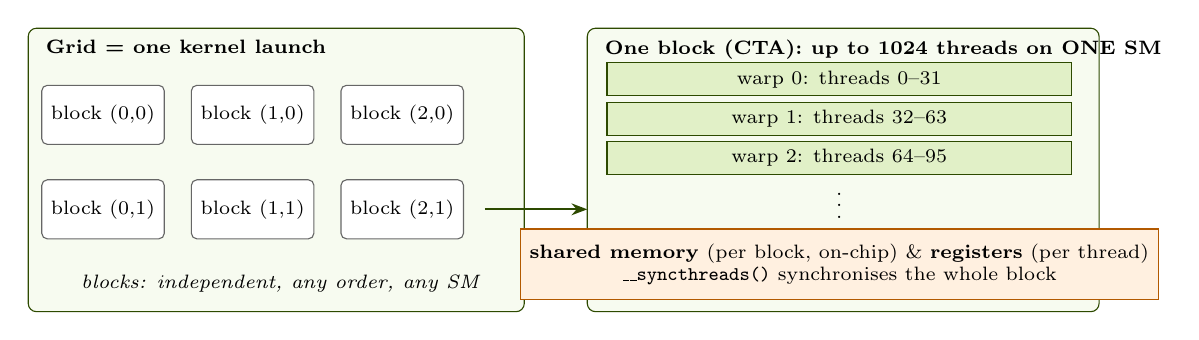
\begin{tikzpicture}[font=\scriptsize,
  blk/.style={draw=black!60,fill=white,rounded corners=2pt,minimum width=1.55cm,minimum height=0.75cm},
  wp/.style={draw=nvdark,fill=nvgreen!22,minimum width=5.9cm,minimum height=0.42cm,inner sep=1pt}]
  \draw[draw=nvdark,fill=nvgreen!6,rounded corners=3pt] (-0.2,-0.3) rectangle (6.1,3.3);
  \node[anchor=north west,font=\scriptsize\bfseries] at (-0.1,3.28) {Grid = one kernel launch};
  \foreach \bi in {0,1,2} {\foreach \bj in {0,1} {
     \node[blk] at (0.75+\bi*1.9,2.2-\bj*1.2) {block (\bi,\bj)};}}
  \node[font=\scriptsize\itshape] at (3.0,0.05) {blocks: independent, any order, any SM};
  \draw[-{Stealth[length=2mm]},thick,nvdark] (5.6,1.0) -- (6.9,1.0);
  \begin{scope}[xshift=7.1cm]
    \draw[draw=nvdark,fill=nvgreen!6,rounded corners=3pt] (-0.2,-0.3) rectangle (6.3,3.3);
    \node[anchor=north west,font=\scriptsize\bfseries] at (-0.1,3.28) {One block (CTA): up to 1024 threads on ONE SM};
    \foreach \bw in {0,1,2} {\node[wp] at (3.0,2.65-\bw*0.5) {warp \bw: threads \the\numexpr 32*\bw\relax--\the\numexpr 32*\bw+31\relax};}
    \node at (3.0,1.15) {$\vdots$};
    \node[draw=orange!70!black,fill=orange!12,minimum width=5.9cm,minimum height=0.9cm,align=center] at (3.0,0.3)
       {\textbf{shared memory} (per block, on-chip) \& \textbf{registers} (per thread)\\ \texttt{\_\_syncthreads()} synchronises the whole block};
  \end{scope}
\end{tikzpicture}
\end{center}

\begin{mustbox}[SIMT in six sentences]
\begin{enumerate}[nosep]
\item A CPU spends transistors on \emph{latency} (big caches, out-of-order cores, branch prediction); a GPU spends them on \emph{throughput}: thousands of simple lanes, and it hides memory latency by switching among many resident threads at zero cost (all their registers stay on chip).
\item You write \textbf{scalar code for one thread}; a launch \texttt{kernel<<<grid, block>>>(args)} creates \texttt{grid} $\times$ \texttt{block} threads. Each finds its work from \texttt{threadIdx}, \texttt{blockIdx}, \texttt{blockDim}, \texttt{gridDim}.
\item The hardware groups 32 consecutive threads into a \textbf{warp}, the unit that is scheduled and issues one instruction at a time (\textbf{SIMT}: single instruction, multiple threads).
\item A \textbf{block} (CTA, cooperative thread array) is resident on \emph{one} SM until it finishes; its threads share \texttt{\_\_shared\_\_} memory and can call \texttt{\_\_syncthreads()}.
\item Blocks of one grid are \textbf{independent}: they may run in any order, concurrently or one after another. The only cross-block communication inside a kernel is atomics and global memory; kernel boundaries are the global barrier. That rule is what lets one binary scale from a 2-SM laptop GPU to a 132-SM datacentre part.
\item Linear thread index: \texttt{i = blockIdx.x * blockDim.x + threadIdx.x}; blocks needed: \texttt{(n + block - 1) / block} (ceiling division); a \textbf{grid-stride loop} (\texttt{for (i = tid; i < n; i += gridDim.x * blockDim.x)}) makes a kernel correct for \emph{any} launch size.
\end{enumerate}
\end{mustbox}
\begin{center}\small
\begin{tabularx}{\textwidth}{@{}L{2.5cm}L{5.6cm}Y@{}}
\toprule
\textbf{Software} & \textbf{Hardware} & \textbf{Limits (public NVIDIA figures; verify in the CUDA C++ Programming Guide)}\\
\midrule
thread & one lane of a warp; owns registers; has a program counter since Volta & up to 255 registers per thread\\
warp & 32 threads, the scheduling/issue unit; a scheduler issues one warp instruction per cycle & warp size 32 on all NVIDIA GPUs to date\\
block / CTA & runs on one SM; own shared memory; barrier & $\le 1024$ threads; dims $\le(1024,1024,64)$; 48~KB static shared memory (up to $\approx$163~KB opt-in on A100)\\
cluster (Hopper+) & blocks co-scheduled on one GPC; \emph{distributed} shared memory among them & portable cluster size $\le 8$\\
grid & all blocks of a launch, spread over SMs & \texttt{gridDim.x} $\le 2^{31}-1$; \texttt{y}, \texttt{z} $\le 65535$\\
SM & 4 sub-partitions, each: warp scheduler, register file, FP32/INT32/FP64 units, tensor core, load/store, special-function unit; unified L1/shared memory & A100: 108 SMs, 2048 threads, 64K registers, up to 164~KB shared per SM; H100 (SXM): 132 SMs, up to 228~KB shared\\
\bottomrule
\end{tabularx}
\end{center}
\textbf{Sources:} NVIDIA \src{https://docs.nvidia.com/cuda/cuda-c-programming-guide/}{CUDA C++ Programming Guide} (chapters ``Programming Model'', ``Hardware Implementation'', appendix ``Compute Capabilities''), the A100 and H100 architecture white papers, and the textbook \emph{Programming Massively Parallel Processors} (Kirk \& Hwu). NVIDIA's developer blog has a good ``CUDA refresher'' series.

\section{Execution: warps, divergence, barriers \prio{3}}
\begin{itemize}[nosep]
\item \textbf{Latency hiding.} A load takes hundreds of cycles; while warp A waits, the scheduler issues instructions from warp B, C\ldots{} This is why GPUs want \emph{many} resident warps (\textbf{occupancy}, Section~\ref{sec:occ}) and why a GPU kernel is fast only if there is enough parallelism and the memory accesses are friendly.
\item \textbf{Divergence.} If lanes of one warp take different sides of a branch, the hardware executes \emph{both} paths one after the other, with the non-participating lanes masked off, and reconverges afterwards. Cost $\approx$ sum of the paths. Branches that are uniform per warp (e.g.\ depending on \texttt{threadIdx.x / 32} or on \texttt{blockIdx}) cost nothing extra. Short \texttt{if}/\texttt{else} bodies are \emph{if-converted} into predicated instructions or \texttt{selp} (we saw this in PTX, Chapter~\ref{ch:ptx}).
\item \textbf{Independent thread scheduling} (Volta, 2017, compute capability 7.0, and later). Every thread has its own program counter and call stack, so divergent threads of a warp may interleave and spin-locks between lanes no longer deadlock the warp. The price: \emph{reconvergence is not guaranteed at the end of an \texttt{if}}. Old ``warp-synchronous'' code that relied on lock-step (e.g.\ the last 32 steps of a reduction without barriers on \texttt{volatile} shared memory) is now \textbf{wrong}; use \texttt{\_\_syncwarp(mask)} or the warp primitives \texttt{\_\_shfl\_*\_sync}, \texttt{\_\_ballot\_sync}, \texttt{\_\_activemask}, \texttt{\_\_any\_sync}, \texttt{\_\_all\_sync}, \texttt{\_\_match\_*\_sync}, which all take an explicit \textbf{member mask}.
\item \textbf{Barrier rules.} \texttt{\_\_syncthreads()} must be reached by every non-exited thread of the block; if it sits inside a branch the condition must be \emph{block-uniform}, else the behaviour is undefined (hang or silent wrong data). The barrier also orders memory: all shared- and global-memory writes before it are visible to the block after it.
\item \textbf{Visibility across blocks.} There is no ordering between blocks within a kernel except through atomics and fences (\texttt{\_\_threadfence()}, \texttt{cuda::atomic\_ref} with scopes \texttt{cta/device/system} --- the PTX \texttt{.scope} qualifiers). \texttt{volatile} is not a synchronisation primitive.
\end{itemize}

\subsection{Worked number: why ``sequential addressing'' wins in a reduction}
A block of 256 threads sums 256 values in shared memory in 8 steps. Version~A (the textbook ``interleaved addressing'') lets thread \texttt{tid} with \texttt{tid \% (2*s) == 0} add \texttt{sdata[tid + s]} for \texttt{s} $=1,2,4,\dots,128$. Version~B (``sequential addressing'') lets \texttt{tid < s} add \texttt{sdata[tid + s]} for \texttt{s} $=128,64,\dots,1$. Count the warps that still have \emph{any} active lane (each such warp occupies an issue slot) and the bank-conflict degree of the \texttt{sdata} accesses:
\needspace{5\baselineskip}
\begin{lstlisting}[language={Python},basicstyle=\ttfamily\scriptsize,title={gpumodel.py: four tiny models}]
"""gpumodel.py -- four tiny models that answer the classic GPU interview questions with numbers."""
from math import ceil

# ---- 1. occupancy (simplified model of compute capability 8.0, e.g. A100) --------------------
SM = dict(max_threads=2048, max_blocks=32, regs=65536, smem=164 * 1024, max_warps=64)

def occupancy(threads, regs_per_thread, smem_per_block=0, sm=SM):
    warps = ceil(threads / 32)
    regs_block = warps * 32 * ceil(regs_per_thread / 8) * 8      # registers are allocated per warp in units of 256
    lim = {
        "threads": sm["max_threads"] // (warps * 32),
        "blocks":  sm["max_blocks"],
        "regs":    sm["regs"] // regs_block if regs_block else 99,
        "smem":    sm["smem"] // smem_per_block if smem_per_block else 99,
    }
    blocks = min(lim.values())
    limiter = [k for k, v in lim.items() if v == blocks][0]
    return blocks, blocks * warps / sm["max_warps"], limiter

# ---- 2. global-memory coalescing: 32-byte sectors touched by one warp ------------------------------
def sectors(addr_of_lane, elem=4):
    s = set()
    for lane in range(32):
        a = addr_of_lane(lane)
        s.update(range(a // 32, (a + elem - 1) // 32 + 1))
    return len(s)

# ---- 3. shared-memory bank conflicts: 32 banks x 4 bytes; same word = broadcast ---------------------
def conflict_degree(word_of_lane, active=range(32)):
    banks = {}
    for lane in active:
        w = word_of_lane(lane)
        banks.setdefault(w % 32, set()).add(w)
    return max(len(v) for v in banks.values())

# ---- 4. how many warps still issue instructions in a step (block of `threads` threads) ----
def warps_active(pred, threads=256):
    return len({t // 32 for t in range(threads) if pred(t)})
\end{lstlisting}
\begin{lstlisting}[language={Python},basicstyle=\ttfamily\scriptsize]
from gpumodel import conflict_degree, warps_active
print("step | A1: tid%(2s)==0      | A2: index=2*s*tid       | B: tid<s, index=tid")
print("     | warps  conflicts     | warps  worst conflict   | warps  worst conflict")
tot = [0, 0, 0]
for k in range(8):
    s = 1 << k                                   # stride used by the interleaved versions at this step
    n = 128 >> k                                 # active threads in A2 and B (they halve every step)
    a1 = warps_active(lambda t: t % (2 * s) == 0)
    c1 = conflict_degree(lambda l: l, active=[l for l in range(32) if l % (2 * s) == 0])
    a2 = warps_active(lambda t: t < n)
    c2 = conflict_degree(lambda l: 2 * s * l, active=range(min(32, n)))
    b = warps_active(lambda t: t < n)
    cb = conflict_degree(lambda l: l, active=range(min(32, n)))
    tot[0] += a1; tot[1] += a2; tot[2] += b
    print(f"  {k}  |  {a1}    {c1}-way          |  {a2}     {c2}-way             |  {b}     {cb}-way")
print(f"total warp-steps: A1={tot[0]}  A2={tot[1]}  B={tot[2]}")
\end{lstlisting}
\needspace{5\baselineskip}
\begin{lstlisting}[style=out,basicstyle=\ttfamily\scriptsize,title={Captured output}]
step | A1: tid%(2s)==0      | A2: index=2*s*tid       | B: tid<s, index=tid
     | warps  conflicts     | warps  worst conflict   | warps  worst conflict
  0  |  8    1-way          |  4     2-way             |  4     1-way
  1  |  8    1-way          |  2     4-way             |  2     1-way
  2  |  8    1-way          |  1     8-way             |  1     1-way
  3  |  8    1-way          |  1     8-way             |  1     1-way
  4  |  8    1-way          |  1     8-way             |  1     1-way
  5  |  4    1-way          |  1     4-way             |  1     1-way
  6  |  2    1-way          |  1     2-way             |  1     1-way
  7  |  1    1-way          |  1     1-way             |  1     1-way
total warp-steps: A1=47  A2=12  B=12
\end{lstlisting}
\textbf{Reading the result.} A1 keeps \emph{every} warp busy (with a few active lanes) for five of the eight steps: 47 warp-steps, caused by \textbf{divergence}. A2 removes the divergence by compacting the active threads (12 warp-steps) but its strided shared-memory index creates up to 8-way \textbf{bank conflicts}. B has A2's 12 warp-steps and no conflicts: that is why every production reduction is built this way (NVIDIA's classic deck \emph{Optimizing Parallel Reduction in CUDA}, Mark Harris, walks through seven such versions and reports a speed-up of about 30$\times$ from first to last on its test GPU). Modern code goes one step further and finishes with warp shuffles (Section~\ref{sec:emu}), skipping shared memory and barriers for the last 32 elements.

\section{Memory hierarchy and access patterns \prio{3}}
\label{sec:mem}
\begin{center}\small
\begin{tabularx}{\textwidth}{@{}L{2.1cm}L{1.9cm}L{4.6cm}Y@{}}
\toprule
\textbf{Space} & \textbf{Scope} & \textbf{Where / speed (order of magnitude)} & \textbf{Rule of thumb}\\
\midrule
registers & thread & on-chip register file; 1 cycle & 255 max per thread; too many $\Rightarrow$ \emph{spills} to local memory and fewer resident warps\\
local memory & thread & off-chip (L1/L2 cached); slow like global & spills and dynamically indexed per-thread arrays; ``local'' means \emph{private}, not fast\\
shared \texttt{\_\_shared\_\_} & block & on-chip SRAM, unified with L1; $\sim$20--30 cycles & 32 banks of 4 bytes; explicit tiling; needs \texttt{\_\_syncthreads()} between writers and readers\\
L1 / L2 & SM / device & L2 shared by all SMs (40~MB on A100); atomics are resolved in L2 & caches, transparent; L2 residency controls exist on newer parts\\
global & grid + host & HBM or GDDR; hundreds of cycles; 1.5--3~TB/s class & \textbf{coalesce}: a warp should touch few 32-byte sectors\\
constant \texttt{\_\_constant\_\_} & grid, read-only & 64~KB + cache & fast when all lanes of a warp read the \emph{same} address (broadcast); serialises otherwise\\
texture / \texttt{\_\_ldg} & grid, read-only & read-only data cache & 2-D/spatial locality, free clamping and interpolation\\
host: pageable, pinned, managed & CPU + GPU & PCIe or NVLink; $\sim$10--50~GB/s link & transfers dominate small kernels; pinned memory enables async copies; \texttt{cudaMallocManaged} migrates pages on demand\\
\bottomrule
\end{tabularx}
\end{center}
\subsection{Coalescing: how many sectors does a warp touch?}
Global memory is served in 32-byte \textbf{sectors} (128-byte cache lines, 4 sectors each). A warp-wide 4-byte load needs at least $32\times4=128$ bytes = 4 sectors; every extra sector is wasted bandwidth. Model: count the sectors touched, for a handful of typical patterns.
\begin{lstlisting}[language={Python},basicstyle=\ttfamily\scriptsize]
from gpumodel import sectors, conflict_degree
patterns = [                                              # (access, byte address touched by lane l)
    ("a[i]                    unit stride",           lambda l: 4 * l),
    ("a[i+1]                  misaligned by one",     lambda l: 4 * (l + 1)),
    ("a[2*i]                  stride 2",              lambda l: 8 * l),
    ("a[4*i]                  stride 4",              lambda l: 16 * l),
    ("a[32*i]                 a column of a matrix",  lambda l: 128 * l),
    ("p[i].x   struct{x,y,z}  array of structures",   lambda l: 12 * l),
    ("p[i].x   struct of 4 floats",                   lambda l: 16 * l),
    ("x[i]     separate arrays   structure of arrays", lambda l: 4 * l),
]
print("-- one warp, one 4-byte load per lane; useful = share of the fetched bytes that are used")
for name, addr in patterns:
    n = sectors(addr)
    print(f"{name:46s} sectors={n:2d}  useful={128 / (32 * n) * 100:5.1f}%")
banks = [                                                 # (access, shared-memory word read by lane l)
    ("s[tid]",                                    lambda l: l),
    ("s[2*tid]",                                  lambda l: 2 * l),
    ("s[4*tid]",                                  lambda l: 4 * l),
    ("s[32*tid]",                                 lambda l: 32 * l),
    ("s[33*tid]",                                 lambda l: 33 * l),
    ("s[0]  all lanes read one word (broadcast)", lambda l: 0),
    ("tile[tid][0]   float tile[32][32]",         lambda l: l * 32),
    ("tile[tid][0]   float tile[32][33] (padded)", lambda l: l * 33),
]
print()
print("-- shared memory: 32 banks x 4 bytes; conflict degree = serialised passes for one warp")
for name, word in banks:
    print(f"{name:46s} {conflict_degree(word)}-way")
\end{lstlisting}
\needspace{5\baselineskip}
\begin{lstlisting}[style=out,basicstyle=\ttfamily\scriptsize,title={Captured output}]
-- one warp, one 4-byte load per lane; useful = share of the fetched bytes that are used
a[i]                    unit stride            sectors= 4  useful=100.0%
a[i+1]                  misaligned by one      sectors= 5  useful= 80.0%
a[2*i]                  stride 2               sectors= 8  useful= 50.0%
a[4*i]                  stride 4               sectors=16  useful= 25.0%
a[32*i]                 a column of a matrix   sectors=32  useful= 12.5%
p[i].x   struct{x,y,z}  array of structures    sectors=12  useful= 33.3%
p[i].x   struct of 4 floats                    sectors=16  useful= 25.0%
x[i]     separate arrays   structure of arrays sectors= 4  useful=100.0%

-- shared memory: 32 banks x 4 bytes; conflict degree = serialised passes for one warp
s[tid]                                         1-way
s[2*tid]                                       2-way
s[4*tid]                                       4-way
s[32*tid]                                      32-way
s[33*tid]                                      1-way
s[0]  all lanes read one word (broadcast)      1-way
tile[tid][0]   float tile[32][32]              32-way
tile[tid][0]   float tile[32][33] (padded)     1-way
\end{lstlisting}
\begin{mustbox}[Two rules that explain most GPU memory performance]
\begin{enumerate}[nosep]
\item \textbf{Make neighbouring threads touch neighbouring addresses} in global memory (the lane index should be the \emph{fastest-varying} index: \texttt{a[row * N + col]} with \texttt{col = threadIdx.x + ...}). Prefer \textbf{structure of arrays} to array of structures; a column walk costs 32 sectors where a row walk costs 4.
\item \textbf{Make neighbouring threads touch different shared-memory banks.} Same bank, different words = serialised; same word = broadcast (free). The classical fix for a transposed or column access is \textbf{padding the row by one word}: \texttt{float tile[32][33]} (used in the transpose kernel below), because the extra word shifts each row by one bank.
\end{enumerate}
\end{mustbox}

\section{Occupancy and the roofline \prio{2}}
\label{sec:occ}
\textbf{Occupancy} = resident warps per SM / maximum warps per SM. A block can become resident only if \emph{all} its needs fit: warp slots (threads), block slots, registers (allocated per warp), and shared memory. The scarcest resource decides. The model below is simplified (it ignores allocation granularities beyond the register unit); NVIDIA's Occupancy Calculator spreadsheet and the API \texttt{cudaOccupancyMaxActiveBlocksPerMultiprocessor} are the exact tools.
\begin{lstlisting}[language={Python},basicstyle=\ttfamily\scriptsize]
from gpumodel import occupancy
configs = [                       # (label, threads/block, registers/thread, shared bytes/block)
    ("256 thr, 32 regs/thr",                    256,  32, 0),
    ("256 thr, 64 regs/thr",                    256,  64, 0),
    ("256 thr, 128 regs/thr",                   256, 128, 0),
    ("256 thr, 32 regs, 48 KB shared/block",    256,  32, 48 * 1024),
    ("1024 thr, 64 regs/thr",                  1024,  64, 0),
    ("32 thr, 32 regs/thr (tiny blocks)",        32,  32, 0),
    ("128 thr, 255 regs/thr",                   128, 255, 0),
]
print("A100-like SM: 2048 threads, 32 blocks, 65536 registers, 164 KB shared memory, 64 warps")
for name, threads, regs, smem in configs:
    blocks, occ, limiter = occupancy(threads, regs, smem)
    print(f"{name:40s} blocks/SM={blocks:2d}  occupancy={occ * 100:5.1f}%  limited by: {limiter}")
\end{lstlisting}
\needspace{5\baselineskip}
\begin{lstlisting}[style=out,basicstyle=\ttfamily\scriptsize,title={Captured output}]
A100-like SM: 2048 threads, 32 blocks, 65536 registers, 164 KB shared memory, 64 warps
256 thr, 32 regs/thr                     blocks/SM= 8  occupancy=100.0%  limited by: threads
256 thr, 64 regs/thr                     blocks/SM= 4  occupancy= 50.0%  limited by: regs
256 thr, 128 regs/thr                    blocks/SM= 2  occupancy= 25.0%  limited by: regs
256 thr, 32 regs, 48 KB shared/block     blocks/SM= 3  occupancy= 37.5%  limited by: smem
1024 thr, 64 regs/thr                    blocks/SM= 1  occupancy= 50.0%  limited by: regs
32 thr, 32 regs/thr (tiny blocks)        blocks/SM=32  occupancy= 50.0%  limited by: blocks
128 thr, 255 regs/thr                    blocks/SM= 2  occupancy= 12.5%  limited by: regs
\end{lstlisting}
\begin{trapbox}[``Maximise occupancy'' is not the goal]
Occupancy is a means to hide latency, not a score. A kernel with 25\% occupancy whose threads each keep several independent loads/FMAs in flight (instruction-level parallelism, more registers per thread) often beats a 100\%-occupancy kernel (V.~Volkov, \emph{Better performance at lower occupancy}, GTC 2010). Conversely, very low occupancy (a few warps) cannot hide a 400-cycle load. Tools: \texttt{-Xptxas -v} (registers, spills, shared bytes), \texttt{\_\_launch\_bounds\_\_(maxThreads, minBlocks)} and \texttt{--maxrregcount} to steer register allocation, Nsight Compute for achieved occupancy.
\end{trapbox}
\subsection{Compute-bound or memory-bound? A 10-line roofline}
\begin{lstlisting}[language={Python},basicstyle=\ttfamily\scriptsize]
bw, peak = 1555e9, 19.5e12        # A100 40GB datasheet: HBM2e bandwidth (B/s), FP32 peak (FLOP/s)
print(f"ridge point = peak / bandwidth = {peak / bw:.1f} FLOP per byte of DRAM traffic\n")
kernels = {
    "vecadd  c=a+b   (1 FLOP per 12 B)": 1 / 12,
    "naive matmul    (2N FLOP per 8N B)": 2 / 8,
    "tiled 16x16     (traffic / 16)":     2 * 16 / 8,
    "tiled 32x32     (traffic / 32)":     2 * 32 / 8,
}
for name, ai in kernels.items():
    rate = min(peak, ai * bw)
    print(f"{name:36s} {ai:5.2f} FLOP/B -> at most {rate / 1e9:7.0f} GFLOP/s = {rate / peak * 100:5.1f}% of peak")
\end{lstlisting}
\needspace{5\baselineskip}
\begin{lstlisting}[style=out,basicstyle=\ttfamily\scriptsize,title={Captured output}]
ridge point = peak / bandwidth = 12.5 FLOP per byte of DRAM traffic

vecadd  c=a+b   (1 FLOP per 12 B)     0.08 FLOP/B -> at most     130 GFLOP/s =   0.7% of peak
naive matmul    (2N FLOP per 8N B)    0.25 FLOP/B -> at most     389 GFLOP/s =   2.0% of peak
tiled 16x16     (traffic / 16)        4.00 FLOP/B -> at most    6220 GFLOP/s =  31.9% of peak
tiled 32x32     (traffic / 32)        8.00 FLOP/B -> at most   12440 GFLOP/s =  63.8% of peak
\end{lstlisting}
Vector addition is hopelessly memory-bound (under 1\% of peak FLOPs): its speed is set by DRAM bandwidth alone, so the only optimisations that matter are coalescing and not moving data (fusion). Tiling cuts the global traffic of a matrix multiply by the tile edge $T$ (each loaded element is reused $T$ times from shared memory), raising intensity to $T/4$ FLOP/B; getting beyond the ridge point needs register tiling and, on recent GPUs, tensor cores --- exactly what libraries such as cuBLAS/CUTLASS do.


% ===== 15b-cuda-lab.tex.in =====
\section{Run CUDA without a GPU: a 60-line emulator \prio{2}}
\label{sec:emu}
\textbf{Idea.} Keep the kernels in a \texttt{.cu} file that begins with \texttt{\#include "cuda\_dual.h"}. Under \textbf{Clang} (\texttt{\_\_CUDA\_\_} defined) the header pulls in the device-only stub from Chapter~\ref{ch:ptx}, so the file compiles to real PTX. Under \textbf{g++} the header turns CUDA into ordinary C++: every CUDA thread of a block becomes a \texttt{std::thread}, \texttt{\_\_syncthreads()} becomes a \texttt{std::barrier}, \texttt{\_\_shared\_\_} becomes a \texttt{static} array (blocks run one at a time, so a static array \emph{is} that block's shared memory), atomics use \texttt{std::atomic\_ref}, and warp shuffles use a per-warp barrier plus exchange slots. Threads that finish call \texttt{arrive\_and\_drop()}, mimicking the hardware rule that exited threads do not block barriers.

\needspace{5\baselineskip}
\begin{lstlisting}[language={[11]C++},basicstyle=\ttfamily\scriptsize,title={cuda\_dual.h (CPU emulation + device-only stub)}]
// cuda_dual.h -- one kernel source, two compilers.
//   clang++ -x cuda --cuda-device-only ...   -> PTX  (device-only stub from the previous chapter)
//   g++ -std=c++20 -pthread                  -> runs on the CPU: every CUDA thread is a std::thread
#pragma once
#ifdef __CUDA__
#include "cuda_stub.h"
__device__ static inline int __shfl_down_sync(unsigned m, int v, int d) { return __nvvm_shfl_sync_down_i32(m, v, d, 0x1f); }
#else
#include <algorithm>
#include <atomic>
#include <barrier>
#include <cstdint>
#include <cstdio>
#include <cstring>
#include <memory>
#include <thread>
#include <vector>

#define __global__
#define __device__
#define __host__
#define __shared__ static          // blocks run one at a time, so a static array *is* that block's shared memory
#define __launch_bounds__(...)

struct dim3 { unsigned x, y, z; dim3(unsigned x_ = 1, unsigned y_ = 1, unsigned z_ = 1) : x(x_), y(y_), z(z_) {} };
inline thread_local dim3 threadIdx;
inline dim3 blockIdx, blockDim, gridDim;

namespace emu {
inline std::barrier<>* block_bar;                              // __syncthreads
inline std::vector<std::unique_ptr<std::barrier<>>> warp_bar;  // __syncwarp and shuffles
inline uint32_t warp_val[32][32];                              // [warp][lane] exchange slots for shuffles
inline thread_local unsigned lin_tid;
}
inline void __syncthreads()                 { emu::block_bar->arrive_and_wait(); }
inline void __syncwarp(unsigned = ~0u)      { emu::warp_bar[emu::lin_tid / 32]->arrive_and_wait(); }
template <class T> inline T __shfl_down_sync(unsigned, T v, int delta, int width = 32) {
    static_assert(sizeof(T) == 4, "4-byte values only");
    unsigned w = emu::lin_tid / 32, lane = emu::lin_tid % 32;
    std::memcpy(&emu::warp_val[w][lane], &v, 4);
    emu::warp_bar[w]->arrive_and_wait();                       // everybody has published its value
    T r = v;                                                   // out-of-range source lane: keep own value
    if ((lane % width) + delta < (unsigned)width) std::memcpy(&r, &emu::warp_val[w][lane + delta], 4);
    emu::warp_bar[w]->arrive_and_wait();                       // everybody has read before slots are reused
    return r;
}
inline int   atomicAdd(int* p, int v)     { return std::atomic_ref<int>(*p).fetch_add(v); }
inline float atomicAdd(float* p, float v) { return std::atomic_ref<float>(*p).fetch_add(v); }

template <class K, class... A>
void launch(dim3 grid, dim3 block, K kernel, A... args) {
    gridDim = grid; blockDim = block;
    const unsigned n = block.x * block.y * block.z, nw = (n + 31) / 32;
    for (unsigned bz = 0; bz < grid.z; ++bz) for (unsigned by = 0; by < grid.y; ++by) for (unsigned bx = 0; bx < grid.x; ++bx) {
        blockIdx = dim3(bx, by, bz);
        std::barrier<> bar(n);
        emu::block_bar = &bar;
        emu::warp_bar.clear();
        for (unsigned w = 0; w < nw; ++w) emu::warp_bar.push_back(std::make_unique<std::barrier<>>(std::min(32u, n - 32 * w)));
        std::vector<std::thread> ts;
        for (unsigned t = 0; t < n; ++t)
            ts.emplace_back([=, &bar] {
                emu::lin_tid = t;
                threadIdx = dim3(t % block.x, (t / block.x) % block.y, t / (block.x * block.y));
                kernel(args...);
                bar.arrive_and_drop();                          // an exited thread no longer blocks barriers
                emu::warp_bar[t / 32]->arrive_and_drop();
            });
        for (auto& th : ts) th.join();
    }
}
#define LAUNCH(kernel, grid, block, ...) launch(dim3(grid), dim3(block), kernel, __VA_ARGS__)
#endif
\end{lstlisting}

\textbf{What the emulator is good for:} checking \emph{logic} (indexing, tiling, grid-stride loops, barriers, atomics) against a CPU reference, running unit tests on a machine without a GPU, and race detection with ThreadSanitizer (Section~\ref{sec:race}). \textbf{What it cannot do:} no lock-step warps (so no divergence or timing information), no GPU memory model (it obeys the C++ one), no performance, one OS thread per CUDA thread (fine for blocks up to 1024). For the real thing, a free Colab GPU runtime has \texttt{nvcc} and an NVIDIA GPU.

\subsection{Six classic kernels, one source}
\texttt{vecadd\_gs} (grid-stride loop), \texttt{reduce\_shfl} (warp-shuffle + shared-memory block reduction), \texttt{matmul\_tiled} (shared-memory tiling), \texttt{transpose32} (padded tile), \texttt{hist\_priv} (privatised histogram with shared-memory atomics), \texttt{scan\_hs} (Hillis--Steele inclusive scan with ping-pong buffers).

\needspace{5\baselineskip}
\begin{lstlisting}[language={CUDA},basicstyle=\ttfamily\scriptsize,title={k15.cu: the kernels}]
#include "cuda_dual.h"
#define TILE 16

__global__ void vecadd_gs(const int* a, const int* b, int* c, int n) {          // grid-stride loop
    for (int i = blockIdx.x * blockDim.x + threadIdx.x; i < n; i += gridDim.x * blockDim.x)
        c[i] = a[i] + b[i];
}

__global__ void reduce_shfl(const int* in, int* out, int n) {                    // block sum: shuffle + shared
    __shared__ int warp_sums[32];
    int i = blockIdx.x * blockDim.x + threadIdx.x;
    int v = (i < n) ? in[i] : 0;
    for (int o = 16; o > 0; o >>= 1) v += __shfl_down_sync(0xffffffffu, v, o);   // sum inside each warp
    int lane = threadIdx.x % 32, warp = threadIdx.x / 32;
    if (lane == 0) warp_sums[warp] = v;
    __syncthreads();
    if (warp == 0) {                                                             // first warp adds the warp sums
        v = (lane < (int)(blockDim.x / 32)) ? warp_sums[lane] : 0;
        for (int o = 16; o > 0; o >>= 1) v += __shfl_down_sync(0xffffffffu, v, o);
        if (lane == 0) atomicAdd(out, v);
    }
}

__global__ void matmul_tiled(const float* A, const float* B, float* C, int N) {  // C = A * B, N multiple of TILE
    __shared__ float As[TILE][TILE];
    __shared__ float Bs[TILE][TILE];
    int row = blockIdx.y * TILE + threadIdx.y, col = blockIdx.x * TILE + threadIdx.x;
    float acc = 0.0f;
    for (int t = 0; t < N / TILE; ++t) {
        As[threadIdx.y][threadIdx.x] = A[row * N + t * TILE + threadIdx.x];
        Bs[threadIdx.y][threadIdx.x] = B[(t * TILE + threadIdx.y) * N + col];
        __syncthreads();                                                         // tile fully loaded
        for (int k = 0; k < TILE; ++k) acc += As[threadIdx.y][k] * Bs[k][threadIdx.x];
        __syncthreads();                                                         // everyone done before overwrite
    }
    C[row * N + col] = acc;
}

__global__ void transpose32(const float* in, float* out, int N) {                // 32x32 tile, padded to dodge bank conflicts
    __shared__ float tile[32][33];
    int x = blockIdx.x * 32 + threadIdx.x, y = blockIdx.y * 32 + threadIdx.y;
    for (int j = 0; j < 32; j += 8) tile[threadIdx.y + j][threadIdx.x] = in[(y + j) * N + x];
    __syncthreads();
    x = blockIdx.y * 32 + threadIdx.x; y = blockIdx.x * 32 + threadIdx.y;       // swapped block coordinates
    for (int j = 0; j < 32; j += 8) out[(y + j) * N + x] = tile[threadIdx.x][threadIdx.y + j];
}

#define BINS 16
__global__ void hist_priv(const unsigned char* data, int* bins, int n) {         // privatised histogram
    __shared__ int local[BINS];
    if (threadIdx.x < BINS) local[threadIdx.x] = 0;
    __syncthreads();
    for (int i = blockIdx.x * blockDim.x + threadIdx.x; i < n; i += gridDim.x * blockDim.x)
        atomicAdd(&local[data[i] % BINS], 1);                                    // contention stays on-chip
    __syncthreads();
    if (threadIdx.x < BINS) atomicAdd(&bins[threadIdx.x], local[threadIdx.x]);   // one global atomic per bin per block
}

__global__ void scan_hs(const int* in, int* out, int n) {                        // Hillis-Steele inclusive scan, one block
    __shared__ int buf[2][256];
    int t = threadIdx.x, cur = 0;
    buf[0][t] = (t < n) ? in[t] : 0;
    __syncthreads();
    for (int d = 1; d < n; d <<= 1) {
        buf[1 - cur][t] = (t >= d) ? buf[cur][t] + buf[cur][t - d] : buf[cur][t];
        cur = 1 - cur;                                                           // ping-pong: read one buffer, write the other
        __syncthreads();
    }
    if (t < n) out[t] = buf[cur][t];
}
\end{lstlisting}

Host harness for the CPU build. \texttt{LAUNCH(kernel, grid, block, args...)} stands for \texttt{kernel<<<grid, block>>>(args...)}; sizes are deliberately awkward (1000 elements, 100-element scan) to test the guards.

\needspace{5\baselineskip}
\begin{lstlisting}[language={[11]C++},basicstyle=\ttfamily\scriptsize,title={host15.cpp: CPU harness}]
#include "k15.cu"
#include <cstdio>
#include <numeric>
#include <vector>
using std::vector;

static void report(const char* name, bool ok) { std::printf("%-14s %s\n", name, ok ? "OK" : "MISMATCH"); }

int main() {
    const int n = 1000;                                    // deliberately not a multiple of the block size
    vector<int> a(n), b(n), c(n, -1), r(n);
    for (int i = 0; i < n; ++i) { a[i] = i; b[i] = 3 * i + 1; r[i] = a[i] + b[i]; }
    LAUNCH(vecadd_gs, 4, 64, a.data(), b.data(), c.data(), n);     // 256 threads cover 1000 elements
    report("vecadd_gs", c == r);

    vector<int> in(n);
    for (int i = 0; i < n; ++i) in[i] = (i * 7) % 13;
    int sum = 0, ref = std::accumulate(in.begin(), in.end(), 0);
    LAUNCH(reduce_shfl, (n + 255) / 256, 256, in.data(), &sum, n);
    std::printf("%-14s emulated=%d reference=%d %s\n", "reduce_shfl", sum, ref, sum == ref ? "OK" : "MISMATCH");

    const int N = 32;
    vector<float> A(N * N), B(N * N), C(N * N), R(N * N, 0.0f);
    for (int i = 0; i < N * N; ++i) { A[i] = float(i % 5); B[i] = float(i % 7 - 3); }
    for (int i = 0; i < N; ++i)
        for (int j = 0; j < N; ++j)
            for (int k = 0; k < N; ++k) R[i * N + j] += A[i * N + k] * B[k * N + j];
    LAUNCH(matmul_tiled, dim3(N / TILE, N / TILE), dim3(TILE, TILE), A.data(), B.data(), C.data(), N);
    report("matmul_tiled", C == R);

    vector<float> T(N * N, 0.0f), RT(N * N);
    for (int i = 0; i < N; ++i)
        for (int j = 0; j < N; ++j) RT[j * N + i] = A[i * N + j];
    LAUNCH(transpose32, dim3(N / 32, N / 32), dim3(32, 8), A.data(), T.data(), N);
    report("transpose32", T == RT);

    vector<unsigned char> d(5000);
    for (size_t i = 0; i < d.size(); ++i) d[i] = (unsigned char)((i * i + 3 * i) & 0xff);
    vector<int> h(BINS, 0), hr(BINS, 0);
    for (unsigned char x : d) hr[x % BINS]++;
    LAUNCH(hist_priv, 3, 128, d.data(), h.data(), (int)d.size());
    report("hist_priv", h == hr);

    vector<int> s(100), sr(100), so(100, -1);
    for (int i = 0; i < 100; ++i) s[i] = i % 4 + 1;
    std::partial_sum(s.begin(), s.end(), sr.begin());
    LAUNCH(scan_hs, 1, 128, s.data(), so.data(), 100);
    report("scan_hs", so == sr);
    return 0;
}
\end{lstlisting}
\begin{lstlisting}[style=shcmd,basicstyle=\ttfamily\scriptsize]
$ g++ -std=c++20 -pthread host15.cpp -o host15 && ./host15
\end{lstlisting}
\begin{lstlisting}[style=out,basicstyle=\ttfamily\scriptsize]
vecadd_gs      OK
reduce_shfl    emulated=6000 reference=6000 OK
matmul_tiled   OK
transpose32    OK
hist_priv      OK
scan_hs        OK
\end{lstlisting}

\subsection{The same kernels as PTX: what a compiler test would look at}
\begin{lstlisting}[style=shcmd,basicstyle=\ttfamily\scriptsize]
$ clang++ -x cuda --cuda-device-only --cuda-gpu-arch=sm_80 -O2 -S k15.cu -o k15.ptx   # then count instructions per kernel
\end{lstlisting}
\begin{lstlisting}[style=out,basicstyle=\ttfamily\scriptsize]
kernel        bar.sync shfl.sync atom.shared atom.global ld.shared st.shared ld.global st.global     fma
vecadd_gs            0         0           0           0         0         0         2         1       0
reduce_shfl          1        10           0           1         1         1         1         0       0
matmul_tiled         2         0           0           0        32         2         2         1      16
transpose32          1         0           0           0         4         4         4         4       0
hist_priv            2         0           1           1         1         1         1         0       0
scan_hs              2         0           0           0         3         2         1         1       0
\end{lstlisting}
Static instruction counts per kernel, read as a verification engineer would: \texttt{matmul\_tiled} has 2 barriers (load phase, compute phase) and the 16-iteration inner loop was fully unrolled into 16 \texttt{fma.rn.f32} (the \texttt{acc += a*b} contraction); \texttt{reduce\_shfl} contains 10 \texttt{shfl.sync} (2 unrolled warp reductions $\times$ 5 steps), one barrier and one global atomic; \texttt{transpose32} has one barrier, four loads and four stores (the \texttt{j} loop unrolled four times, no branches); \textbf{\texttt{hist\_priv}} shows one \texttt{atom.shared} and one \texttt{atom.global}: the source used the same generic \texttt{atomicAdd(int*, int)} for both, and the compiler's \emph{address-space inference} proved which memory each pointer targets. A bug in that inference is exactly the kind of defect a GPU-compiler test suite is written to catch. The IR also shows the attribute that protects barriers:
\begin{lstlisting}[style=shcmd,basicstyle=\ttfamily\scriptsize]
$ clang++ ... -S -emit-llvm k15.cu | grep -E 'barrier0|attributes #2'
\end{lstlisting}
\begin{lstlisting}[language={LLVMIR},style=out,basicstyle=\ttfamily\scriptsize]
declare void @llvm.nvvm.barrier0() #2
attributes #2 = { convergent nocallback nounwind }
\end{lstlisting}
\textbf{\texttt{convergent}} means ``this operation communicates with other threads that must execute it together'': an optimiser may not make it \emph{control-dependent on more conditions} than before (no jump threading or sinking of a barrier or shuffle into a divergent branch) --- a rule every LLVM-based GPU compiler must implement and test.

\section{Race detection with ThreadSanitizer \prio{2}}
\label{sec:race}
On a GPU the tool is \texttt{compute-sanitizer --tool racecheck} (and \texttt{synccheck} for barrier misuse, \texttt{memcheck} for out-of-bounds, \texttt{initcheck} for uninitialised memory). In our emulator the C++ ThreadSanitizer does the same job for shared-memory bugs, because the barrier is the only thing ordering the threads of a block. Two classic bugs, each with a one-line description:

\needspace{5\baselineskip}
\begin{lstlisting}[language={CUDA},basicstyle=\ttfamily\scriptsize,title={kbug.cu: two kernels with a missing barrier}]
#include "cuda_dual.h"
__global__ void scan_inplace_bug(const int* in, int* out, int n) {     // BUG: in-place Hillis-Steele, single buffer
    __shared__ int x[256];
    int t = threadIdx.x;
    x[t] = (t < n) ? in[t] : 0;
    __syncthreads();
    for (int d = 1; d < n; d <<= 1) {
        int v = (t >= d) ? x[t - d] : 0;      // read a neighbour's slot ...
        x[t] += v;                            // ... while that neighbour may already be overwriting it
        __syncthreads();
    }
    if (t < n) out[t] = x[t];
}
__global__ void tile_sync_bug(const float* A, float* out) {            // BUG: second barrier missing
    __shared__ float tile[32];
    float acc = 0;
    for (int t = 0; t < 4; ++t) {
        tile[threadIdx.x] = A[t * 32 + threadIdx.x];
        __syncthreads();
        acc += tile[(threadIdx.x + 1) % 32];  // read the neighbour's element
        /* missing __syncthreads() here */
    }
    out[threadIdx.x] = acc;
}
\end{lstlisting}



\begin{lstlisting}[style=shcmd,basicstyle=\ttfamily\scriptsize]
$ g++ -std=c++20 -g -fsanitize=thread hostbug.cpp && ./a.out   # report the kernel names only
\end{lstlisting}
\begin{lstlisting}[style=out,basicstyle=\ttfamily\scriptsize]
ThreadSanitizer: data race in kernel scan_inplace_bug
ThreadSanitizer: data race in kernel tile_sync_bug
--- number of ThreadSanitizer reports for the six correct kernels (host15.cpp):
0
\end{lstlisting}
\textbf{Reading it.} The in-place scan reads \texttt{x[t-d]} while thread \texttt{t-d} may already be writing it in the same step (a read-after-write hazard inside one iteration, fixed by the ping-pong buffer in \texttt{scan\_hs} or by a barrier between the read and the write); the tile kernel overwrites \texttt{tile[]} for the next \texttt{t} while a slow neighbour is still reading the old value. The correct kernels produce \textbf{zero} reports. On the GPU a hazard like this may give correct answers 999 times out of 1000 --- which is why \emph{tools} rather than test runs find them.

\section{The CUDA bug catalogue \prio{2}}
\begin{center}\small
\begin{tabularx}{\textwidth}{@{}L{4.1cm}L{3.9cm}Y@{}}
\toprule
\textbf{Bug} & \textbf{Symptom} & \textbf{Catch / fix}\\
\midrule
missing barrier between shared-memory writers and readers (or before the buffer is overwritten) & intermittent wrong results; right 999 times in 1000 & \texttt{compute-sanitizer --tool racecheck}; TSan on the emulator; barrier after each producer phase \emph{and} before reuse\\
\texttt{\_\_syncthreads()} inside a branch that is not block-uniform, or after a thread-dependent early \texttt{return} & hang or garbage; undefined behaviour & \texttt{--tool synccheck}; guard the \emph{work}, not the barrier\\
no \texttt{if (i < n)} guard, or grid size rounded \emph{down} & out-of-bounds writes; tail elements never computed & \texttt{--tool memcheck}; \texttt{(n + block - 1) / block}\\
32-bit index overflow (\texttt{row * N + col}, \texttt{int} loop counter) & wrong addresses for big arrays & use \texttt{size\_t} / \texttt{long long}; see \texttt{mul.wide} in Chapter~\ref{ch:ptx}\\
warp-synchronous code without \texttt{\_\_syncwarp}, or a wrong shuffle/ballot mask & rare wrong results on Volta and later & always pass the real participation mask; full mask \texttt{0xffffffff} only if the whole warp executes the call\\
non-atomic read-modify-write on shared data (\texttt{count++}) & lost updates & \texttt{atomicAdd}, or a reduction\\
float \texttt{atomicAdd} or a different summation order & results differ in the last bits between runs/devices & not a bug: floating-point addition is not associative; compare with a tolerance, or use a fixed-order tree\\
uninitialised shared or local memory & results change from launch to launch & \texttt{--tool initcheck}; (our emulator's static arrays start at zero and \emph{hide} this bug)\\
host pointer used on the device or vice versa; forgotten copy & \texttt{invalid argument}, zeros, crashes & name pointers \texttt{h\_x}/\texttt{d\_x}; check every API call\\
errors seen late: a launch is \emph{asynchronous} & failure surfaces at the next API call that synchronises & \texttt{CHECK(cudaGetLastError())} after the launch; \texttt{cudaDeviceSynchronize()} while debugging\\
too many resources (\texttt{1024} threads $\times$ many registers; too much shared memory) & \texttt{too many resources requested for launch} & smaller block, \texttt{\_\_launch\_bounds\_\_}, \texttt{--maxrregcount}\\
\bottomrule
\end{tabularx}
\end{center}

\section{Host-side API cheat sheet \prio{2}}
The standard pattern (not compiled here: there is no CUDA SDK in the sandbox; the device half is exactly what we compiled above):
\needspace{5\baselineskip}
\begin{lstlisting}[language={CUDA},basicstyle=\ttfamily\scriptsize,title={saxpy.cu: allocate, copy, launch, check, copy back}]
#include <cstdio>
#include <cstdlib>
#include <cuda_runtime.h>
#define CHECK(call) do { cudaError_t e = (call); if (e != cudaSuccess) {                        \
    std::fprintf(stderr, "%s:%d: %s\n", __FILE__, __LINE__, cudaGetErrorString(e)); std::exit(1); } } while (0)

__global__ void saxpy(int n, float a, const float* x, float* y) {
    int i = blockIdx.x * blockDim.x + threadIdx.x;
    if (i < n) y[i] = a * x[i] + y[i];
}

int main() {
    const int n = 1 << 20;
    const size_t bytes = n * sizeof(float);
    float *hx = (float*)std::malloc(bytes), *hy = (float*)std::malloc(bytes), *dx, *dy;
    for (int i = 0; i < n; ++i) { hx[i] = 1.0f; hy[i] = 2.0f; }

    CHECK(cudaMalloc(&dx, bytes));  CHECK(cudaMalloc(&dy, bytes));
    CHECK(cudaMemcpy(dx, hx, bytes, cudaMemcpyHostToDevice));
    CHECK(cudaMemcpy(dy, hy, bytes, cudaMemcpyHostToDevice));

    int block = 256, grid = (n + block - 1) / block;     // ceiling division
    saxpy<<<grid, block>>>(n, 3.0f, dx, dy);              // asynchronous
    CHECK(cudaGetLastError());                             // launch-configuration errors
    CHECK(cudaDeviceSynchronize());                        // errors raised while the kernel ran

    CHECK(cudaMemcpy(hy, dy, bytes, cudaMemcpyDeviceToHost));
    std::printf("y[0] = %f (expect 5)\n", hy[0]);
    cudaFree(dx); cudaFree(dy); std::free(hx); std::free(hy);
}
\end{lstlisting}
\begin{center}\small
\begin{tabularx}{\textwidth}{@{}L{5.4cm}Y@{}}
\toprule
\textbf{API} & \textbf{Meaning}\\
\midrule
\texttt{cudaMalloc}, \texttt{cudaFree}, \texttt{cudaMemcpy(dst, src, bytes, kind)} & device allocation; blocking copy (\texttt{cudaMemcpyHostToDevice}, \texttt{cudaMemcpyDeviceToHost}, ...)\\
\texttt{cudaMallocHost}, \texttt{cudaMemcpyAsync(..., stream)} & pinned host memory and asynchronous copies that can overlap with kernels\\
\texttt{cudaMallocManaged}, \texttt{cudaMemPrefetchAsync} & unified (managed) memory: one pointer valid on host and device, pages migrate on demand\\
\texttt{cudaStream\_t}, \texttt{cudaStreamCreate}, \texttt{<<<grid, block, shmem, stream>>>} & independent queues of work; same-stream work is ordered, different streams may overlap\\
\texttt{cudaEvent\_t}, \texttt{cudaEventRecord}, \texttt{cudaEventElapsedTime} & GPU-side timestamps: the right way to time kernels (host timers miss asynchrony)\\
\texttt{cudaDeviceSynchronize}, \texttt{cudaStreamSynchronize} & host waits for all (or one stream's) work\\
\texttt{cudaGetLastError}, \texttt{cudaGetErrorString}, \texttt{cudaGetDeviceProperties} & error handling; query SM count, shared memory, compute capability\\
occupancy API & \texttt{cudaOccupancyMaxActiveBlocksPerMultiprocessor} gives the exact number of resident blocks for a given kernel and block size\\
\bottomrule
\end{tabularx}
\end{center}
\textbf{Build and inspect:} \texttt{nvcc -O2 -arch=sm\_80 -lineinfo saxpy.cu -o saxpy}; \texttt{cuobjdump -sass -ptx saxpy} shows what is inside; \texttt{compute-sanitizer ./saxpy}; \texttt{ncu ./saxpy} (Nsight Compute: per-kernel hardware counters), \texttt{nsys profile ./saxpy} (Nsight Systems: timeline).

\section{Recent hardware features: the one-line versions \prio{1}}
\begin{center}\small
\begin{tabularx}{\textwidth}{@{}L{3.3cm}L{2.5cm}Y@{}}
\toprule
\textbf{Feature} & \textbf{Since} & \textbf{What it is, and why compiler people care}\\
\midrule
\textbf{Tensor Cores} (\texttt{wmma}, \texttt{mma.sync}, \texttt{wgmma}) & Volta (2017); 4th gen Hopper & small matrix-multiply-accumulate per warp (or warp group), mixed precision: FP16/BF16/TF32/INT8/FP8 inputs, wider accumulators; new PTX instruction families with fragment register layouts that the register allocator and scheduler must respect\\
\textbf{Asynchronous copy}: \texttt{cp.async}; \textbf{TMA} (tensor memory accelerator) & Ampere; Hopper & copy global$\to$shared without staging through registers; TMA moves whole multi-dimensional tiles; synchronised with \texttt{mbarrier}s: new ordering rules to verify\\
\textbf{Thread block clusters}, distributed shared memory & Hopper & blocks of a cluster can read each other's shared memory: a new PTX memory scope (\texttt{.cluster})\\
\textbf{Cooperative Groups} & CUDA 9 & named groups (tile, warp, block, grid) with \texttt{sync()}, \texttt{reduce()}\ldots; compile down to \texttt{bar}/\texttt{shfl}; grid-wide sync needs a cooperative launch\\
\textbf{CUDA Graphs} & CUDA 10 & record a DAG of kernels/copies once and replay it with low CPU overhead\\
\textbf{Dynamic parallelism} & CUDA 5 & kernels launching kernels\\
\textbf{MIG, MPS} & Ampere; Kepler & hardware partitioning / software sharing of one GPU among tenants\\
\textbf{Lower-precision formats} & Hopper onwards (FP8; newer parts add narrower formats) & more types in PTX and in NVVM IR; more FP semantics (rounding, saturation, NaN handling) for tests to cover\\
\bottomrule
\end{tabularx}
\end{center}
\textbf{Ecosystem names worth recognising:} cuBLAS, cuDNN, CUTLASS (templated GEMM building blocks), CUB and Thrust (parallel primitives), NCCL (multi-GPU collectives), TensorRT, NVRTC, \textbf{Triton} (a Python DSL whose compiler lowers to LLVM IR and PTX), Nsight Systems/Compute, \texttt{compute-sanitizer}.

\begin{srcbox}[Why the compiler-verification team cares about all of this]
Each item above is a place where a GPU compiler can be wrong, and a test generator or a hand-written kernel can show it: \textbf{barriers and \texttt{convergent} operations} moved across divergent control flow; \textbf{address-space inference} (generic $\to$ shared/global/local); \textbf{if-conversion and divergence analysis} (\texttt{selp}, \texttt{bra.uni}); \textbf{memory ordering} around \texttt{bar.sync}, fences, atomics and scopes; \textbf{FP contraction, flush-to-zero and rounding} flags (\texttt{--fmad}, \texttt{-ftz}, \texttt{-prec-div}); \textbf{integer semantics} (\texttt{nsw} assumptions on index arithmetic, 32-bit vs 64-bit address math); \textbf{register allocation and spills} under \texttt{\_\_launch\_bounds\_\_}; \textbf{vectorised loads} (\texttt{ld.v4}) that need alignment proofs; \textbf{warp-level primitives} with partial masks. Chapter~\ref{ch:verif} turns this list into a test plan.
\end{srcbox}

\section{Practice questions \prio{2}}
\begin{qn}Define thread, warp, block and grid. Why should the block size be a multiple of 32, and what is a sensible default?\end{qn}
\begin{ans}A \emph{thread} runs the kernel body on its own registers; a \emph{warp} is 32 consecutive threads issued together; a \emph{block} is a group of up to 1024 threads that lives on one SM, shares shared memory and can synchronise; a \emph{grid} is all blocks of a launch. Warps are the scheduling unit, so a block of 100 threads still occupies 4 warps and wastes 28 lanes. 128 or 256 is a good default: enough warps to hide latency, a divisor of the 2048-thread SM limit, and small enough that registers and shared memory still allow several resident blocks.\end{ans}
\begin{qn}What is warp divergence, when is it free, and how do you reduce it?\end{qn}
\begin{ans}Lanes of one warp taking different paths: the hardware runs the paths serially with masks, so cost $\approx$ sum of paths. Free when the condition is uniform across the warp (e.g.\ \texttt{threadIdx.x / 32}, \texttt{blockIdx}-dependent) and when the compiler predicates a short body. Reduce it by regrouping work so that neighbouring threads take the same path (sort/bin inputs, compact active threads as in reduction version B), and by replacing branches with arithmetic or \texttt{select}.\end{ans}
\begin{qn}Difference between \texttt{\_\_syncthreads()}, \texttt{\_\_syncwarp()}, \texttt{\_\_threadfence()} and \texttt{cudaDeviceSynchronize()}?\end{qn}
\begin{ans}\texttt{\_\_syncthreads()}: barrier for all threads of the block, with memory ordering for shared and global writes among them. \texttt{\_\_syncwarp(mask)}: barrier and memory ordering among the named lanes of one warp. \texttt{\_\_threadfence()}: only orders the calling thread's memory writes as seen by other threads of the device --- \emph{no} waiting. \texttt{cudaDeviceSynchronize()}: host-side call that blocks until all previously issued device work is finished.\end{ans}
\begin{qn}Why does the tiled matrix multiply have two \texttt{\_\_syncthreads()} per tile?\end{qn}
\begin{ans}The first makes sure the whole tile has been loaded before any thread starts using it; the second makes sure all threads have finished using the tile before the next iteration overwrites it. Dropping the second one is the race that ThreadSanitizer flagged in \texttt{tile\_sync\_bug}.\end{ans}
\begin{qn}A kernel uses 64 registers per thread, 256 threads per block and no shared memory. What is the occupancy on an A100-like SM, and what would you try?\end{qn}
\begin{ans}Registers per block $=256\times64=16384$, so $65536/16384=4$ blocks $=1024$ threads $=50\%$ (table above). Try \texttt{--maxrregcount=32} or \texttt{\_\_launch\_bounds\_\_(256, 8)} only if profiling shows latency stalls; the forced register cut may cause spills that cost more than the extra occupancy gains.\end{ans}
\begin{qn}Why can the sum of a float array differ between CPU and GPU, and between two GPU runs?\end{qn}
\begin{ans}Floating-point addition is not associative; the GPU adds in a tree (and with \texttt{atomicAdd} in an order that depends on scheduling), the CPU adds left to right. Results are all valid approximations. Compare with a relative tolerance, or use a fixed reduction tree (and integers or Kahan summation) for bit-reproducible results.\end{ans}
\begin{qn}What is a bank conflict? Show a fix.\end{qn}
\begin{ans}Two or more lanes of a warp access \emph{different} 32-bit words in the same one of the 32 shared-memory banks in one instruction; the accesses are serialised. Same word = broadcast, no conflict. Column access to a \texttt{float tile[32][32]} is 32-way; padding the declaration to \texttt{tile[32][33]} makes it conflict-free (checked in the model above and used in \texttt{transpose32}).\end{ans}
\begin{qn}Coalesced vs.\ uncoalesced: how many 32-byte sectors does \texttt{a[32*i]} touch per warp, and what is the fix?\end{qn}
\begin{ans}32 sectors for 128 useful bytes (12.5\% efficiency) versus 4 for \texttt{a[i]}. Fix: change the data layout (structure of arrays), swap loop and thread indexing so the lane index is the fastest-varying one, or stage a tile through shared memory so the global loads are coalesced and the strided access happens on-chip.\end{ans}
\begin{qn}PTX versus SASS versus cubin, and what does \texttt{-arch=sm\_80} do?\end{qn}
\begin{ans}PTX is NVIDIA's virtual ISA (text, forward compatible, JIT-able); SASS is the native machine code of one GPU generation; a cubin is the ELF container with SASS. \texttt{-arch=sm\_80} is shorthand for \texttt{-gencode arch=compute\_80,code=[sm\_80,compute\_80]}: emit SASS for sm\_80 and also embed compute\_80 PTX so newer GPUs can JIT it.\end{ans}
\begin{qn}You are asked to test that a GPU compiler handles \texttt{\_\_syncthreads()} correctly. What do you write?\end{qn}
\begin{ans}Kernels where the barrier sits in straight-line code, in uniform loops, in nested uniform branches and after a thread-dependent \emph{value} (but not a thread-dependent \emph{control path}); each has a CPU reference (the emulator above can serve). Compile at several optimisation levels and \texttt{sm\_} targets, run, compare outputs (differential testing), check the PTX with FileCheck for the expected \texttt{bar.sync} count and position, run \texttt{racecheck}/\texttt{synccheck}, and add negative tests for transformations that must \emph{not} happen (barrier sunk into a divergent branch). Chapters~\ref{ch:verif} and~\ref{ch:pylab} build such a harness.\end{ans}


% ===== 16-parallel.tex.in =====
\chapter{Parallel Programming: Threads, Atomics, OpenMP, Patterns}
\label{ch:par}

\begin{chapbox}
\textbf{Priority \prio{2} (the job description lists ``parallel programming'' as a stand-out skill). Time: 60 min.} Everything here was compiled and run in the sandbox (4 virtual CPUs, GCC 13, ThreadSanitizer, OpenMP, Python 3.13). \textbf{Timings are real but machine-dependent}: read them for the \emph{ratio}, not the absolute numbers; counts of race outcomes vary from run to run by design. Chapter~\ref{ch:cuda} applied the same ideas (races, barriers, atomics, reductions, scans) to GPUs.
\end{chapbox}

\section{Vocabulary and speed-up laws \prio{2}}
\begin{itemize}[nosep]
\item \textbf{Concurrency} = several tasks in progress, structured so they \emph{may} interleave (one core is enough); \textbf{parallelism} = several tasks executing \emph{simultaneously} (needs several execution units).
\item \textbf{Flynn's taxonomy:} SISD (one instruction stream, one data stream: classic CPU core), \textbf{SIMD} (one instruction on many data: AVX/NEON vector units), MISD (rare), \textbf{MIMD} (independent cores: multicore CPUs, clusters). A GPU is \textbf{SIMT}: SIMD hardware presented as many scalar threads with per-thread state.
\item \textbf{Kinds of parallelism:} \emph{data} (same operation on many elements: GPU kernels, \texttt{\#pragma omp parallel for}), \emph{task} (different jobs: compile 100 files at once), \emph{pipeline} (stages in series, each busy on a different item).
\item \textbf{Speed-up} $S(p)=T_1/T_p$, \textbf{efficiency} $E=S/p$. \textbf{Amdahl:} if a fraction $f$ of the work is parallelisable, $S(p)\le 1/\big((1-f)+f/p\big)$, so the serial part caps the speed-up at $1/(1-f)$. \textbf{Gustafson:} if the problem grows with the machine, scaled speed-up is $(1-f)+fp$.
\item \textbf{Work and span:} $W=T_1$ (total operations), $S_\infty=T_\infty$ (critical-path length, ``depth''); \textbf{Brent's bound} $T_p\le W/p+S_\infty$; available parallelism $=W/S_\infty$. A good parallel algorithm has work close to the best sequential algorithm and a small span.
\end{itemize}
\begin{lstlisting}[language={Python},basicstyle=\ttfamily\scriptsize]
from math import log2
from itertools import accumulate

def amdahl(f, p):    return 1 / ((1 - f) + f / p)            # fixed problem size
def gustafson(f, p): return (1 - f) + f * p                  # problem grows with p

print("Amdahl speed-up S(p) = 1/((1-f)+f/p)")
print("   f      p=4     p=16     p=64   p=1024   limit 1/(1-f)")
for f in (0.50, 0.90, 0.95, 0.99):
    row = "  ".join(f"{amdahl(f, p):7.2f}" for p in (4, 16, 64, 1024))
    print(f" {f:4.2f}  {row}   {1 / (1 - f):8.1f}")
print(f"\nGustafson with f=0.95, p=64: {gustafson(0.95, 64):.1f}   (Amdahl, same f and p: {amdahl(0.95, 64):.1f})")

# ---- prefix sum (scan): work = number of additions, span = number of parallel steps ----------------
def hillis_steele(a):                                         # inclusive; every step adds a shifted copy
    a, work, steps, d = list(a), 0, 0, 1
    while d < len(a):
        a = [a[i] + a[i - d] if i >= d else a[i] for i in range(len(a))]
        work += len(a) - d; steps += 1; d *= 2
    return a, work, steps

def blelloch(a):                                              # exclusive; up-sweep then down-sweep; n = 2**k
    a, n, work, steps, d = list(a), len(a), 0, 0, 1
    while d < n:                                              # up-sweep: build partial sums (a reduction tree)
        for i in range(2 * d - 1, n, 2 * d): a[i] += a[i - d]; work += 1
        steps += 1; d *= 2
    a[n - 1] = 0
    d = n // 2
    while d >= 1:                                             # down-sweep: distribute the prefixes
        for i in range(2 * d - 1, n, 2 * d): a[i - d], a[i] = a[i], a[i] + a[i - d]; work += 1
        steps += 1; d //= 2
    return a, work, steps

n = 1024
data = [(i * 7) % 10 for i in range(n)]
ref = list(accumulate(data))
hs, w1, s1 = hillis_steele(data)
bl, w2, s2 = blelloch(data)
assert hs == ref and [x + y for x, y in zip(bl, data)] == ref                 # both verified against itertools
print(f"\nscan of n={n}: sequential work={n - 1} span={n - 1} | Hillis-Steele work={w1} span={s1} | Blelloch work={w2} span={s2}")
N, p = 2 ** 20, 1024                                                          # closed forms, checked above for n=1024
W_hs, S_hs, W_bl, S_bl = N * int(log2(N)) - N + 1, int(log2(N)), 2 * (N - 1), 2 * int(log2(N))
print(f"Brent bound T_p <= W/p + S for n=2**20, p={p}: Hillis-Steele {W_hs / p + S_hs:.0f}, Blelloch {W_bl / p + S_bl:.0f}")
\end{lstlisting}
\needspace{5\baselineskip}
\begin{lstlisting}[style=out,basicstyle=\ttfamily\scriptsize,title={Captured output}]
Amdahl speed-up S(p) = 1/((1-f)+f/p)
   f      p=4     p=16     p=64   p=1024   limit 1/(1-f)
 0.50     1.60     1.88     1.97     2.00        2.0
 0.90     3.08     6.40     8.77     9.91       10.0
 0.95     3.48     9.14    15.42    19.64       20.0
 0.99     3.88    13.91    39.26    91.18      100.0

Gustafson with f=0.95, p=64: 60.8   (Amdahl, same f and p: 15.4)

scan of n=1024: sequential work=1023 span=1023 | Hillis-Steele work=9217 span=10 | Blelloch work=2046 span=20
Brent bound T_p <= W/p + S for n=2**20, p=1024: Hillis-Steele 19476, Blelloch 2088
\end{lstlisting}
\textbf{Read-out.} With 95\% parallel code, 1024 processors give 19.6$\times$, never more than 20$\times$ (Amdahl). A prefix sum shows why \emph{work-efficiency} matters: Hillis--Steele has the shorter span (10 steps) but does $n\log_2 n$ additions (what \texttt{scan\_hs} in Chapter~\ref{ch:cuda} does inside one block); Blelloch has twice the span but only $2(n-1)$ additions, which wins as soon as there are fewer processors than elements --- the Brent bound above predicts $\sim$9$\times$ fewer time steps for it.

\section{Data races, mutexes and atomics \prio{3}}
\begin{defbox}[Data race (C/C++ definition)]
Two threads access the \emph{same memory location}, at least one access is a \emph{write}, at least one is not atomic, and nothing orders them (no \emph{happens-before} edge from a mutex, atomic acquire/release, thread start/join\ldots). A data race is \textbf{undefined behaviour}: not ``a slightly wrong number'' but a licence for the compiler to assume it never happens (it may keep the variable in a register across the whole loop, hoist loads, tear writes). A \emph{race condition} is the broader logic bug where the result depends on timing; it can exist even without a data race.
\end{defbox}
\needspace{5\baselineskip}
\begin{lstlisting}[language={[11]C++},title={race.cpp}]
#include <cstdio>
#include <thread>
int counter = 0;                                  // plain int: concurrent increments are a data race
void work() { for (int i = 0; i < 1000000; ++i) counter++; }
int main() {
    std::thread a(work), b(work);
    a.join(); b.join();
    std::printf("expected 2000000, got %d\n", counter);
}
\end{lstlisting}
\begin{lstlisting}[style=shcmd]
$ g++ -O0 -pthread race.cpp && ./a.out      # then again under ThreadSanitizer: g++ -g -fsanitize=thread race.cpp
\end{lstlisting}
\begin{lstlisting}[style=out]
expected 2000000, got 1094220
SUMMARY: ThreadSanitizer: data race race.cpp:4 in work()
WARNING: ThreadSanitizer: data race 
\end{lstlisting}
A large share of the increments is lost (the number changes on every run), because \texttt{counter++} is three steps (load, add, store) and two threads interleave them. ThreadSanitizer (\texttt{-fsanitize=thread}) names the racing line without needing the bad interleaving to show up in the result --- it is the first tool to reach for. Three correct ways to sum an array of 20 million ones with 4 threads:
\begin{lstlisting}[language={[11]C++},basicstyle=\ttfamily\scriptsize]
#include <atomic>
#include <chrono>
#include <cstdio>
#include <mutex>
#include <thread>
#include <vector>
using Clock = std::chrono::steady_clock;
template <class Body, class Result>
void run(const char* name, const std::vector<int>& data, Body body, Result result) {
    auto t0 = Clock::now();
    std::vector<std::thread> ts;
    for (int t = 0; t < 4; ++t) ts.emplace_back([&, t] { body(t, data.size() / 4); });
    for (auto& th : ts) th.join();
    double ms = std::chrono::duration<double, std::milli>(Clock::now() - t0).count();
    std::printf("%-42s sum=%ld  %8.1f ms\n", name, (long)result(), ms);
}
int main() {
    std::vector<int> data(20000000, 1);
    long locked = 0, partial = 0;
    std::mutex m;
    std::atomic<long> atom{0};
    run("lock a mutex for every element", data, [&](int t, size_t n) {
        for (size_t i = t * n; i < (t + 1) * n; ++i) { std::lock_guard<std::mutex> g(m); locked += data[i]; } },
        [&] { return locked; });
    run("atomic fetch_add for every element", data, [&](int t, size_t n) {
        for (size_t i = t * n; i < (t + 1) * n; ++i) atom.fetch_add(data[i], std::memory_order_relaxed); },
        [&] { return atom.load(); });
    run("private partial sum, one lock at the end", data, [&](int t, size_t n) {
        long local = 0;
        for (size_t i = t * n; i < (t + 1) * n; ++i) local += data[i];
        std::lock_guard<std::mutex> g(m); partial += local; },
        [&] { return partial; });
}
\end{lstlisting}
\needspace{5\baselineskip}
\begin{lstlisting}[style=out,basicstyle=\ttfamily\scriptsize,title={Captured output (4 threads, 20 million elements)}]
lock a mutex for every element             sum=20000000    1378.2 ms
atomic fetch_add for every element         sum=20000000     755.8 ms
private partial sum, one lock at the end   sum=20000000       5.2 ms
\end{lstlisting}
All three are exact; the ranking is the lesson: \textbf{contention is the cost}. A mutex per element serialises everything and adds lock overhead; an atomic is cheaper but still bounces one cache line between cores; private partial sums touch shared state once per thread --- the same structure as a GPU reduction (per-thread, then per-warp, then per-block, then global).

\begin{mustbox}[Mutex, atomic, or neither?]
\begin{itemize}[nosep]
\item \textbf{Prefer no sharing:} give each thread its own data and combine once (map--reduce). \textbf{Then prefer a mutex} (\texttt{std::lock\_guard}, \texttt{std::scoped\_lock}, RAII: unlock on every path, including exceptions). \textbf{Atomics} only for simple counters/flags or when you can prove the memory ordering.
\item A \textbf{mutex} gives mutual exclusion \emph{and} a happens-before edge (unlock $\to$ next lock). A \textbf{semaphore} counts permits and need not be owned by the thread that releases it. A \textbf{spinlock} busy-waits: good only for very short critical sections on a dedicated core. A \textbf{reader--writer lock} (\texttt{std::shared\_mutex}) lets many readers in.
\item \texttt{volatile} is \textbf{not} a synchronisation tool in C/C++ (no atomicity, no ordering between threads); use \texttt{std::atomic}. \texttt{std::shared\_ptr}'s \emph{control block} is thread-safe, the pointee is not.
\item \textbf{Thread basics:} every \texttt{std::thread} must be \texttt{join()}ed or \texttt{detach()}ed before destruction (else \texttt{std::terminate}); prefer \texttt{std::jthread} (C++20, joins automatically, supports stop tokens); exceptions do not cross threads (use \texttt{std::future}/\texttt{std::promise}, \texttt{std::async}). C++20 also adds \texttt{std::latch}, \texttt{std::barrier}, \texttt{std::counting\_semaphore}.
\end{itemize}
\end{mustbox}

\section{Deadlock, livelock, starvation \prio{2}}
\textbf{Deadlock} needs all four Coffman conditions: \emph{mutual exclusion}, \emph{hold and wait}, \emph{no preemption}, \emph{circular wait}. Break one: acquire locks in a \textbf{global order}, take all at once with \texttt{std::scoped\_lock(a, b)} (a deadlock-avoidance algorithm), use \texttt{try\_lock} with back-off, or avoid holding locks while calling unknown code. \textbf{Livelock:} threads keep reacting to each other and make no progress (two people stepping aside in a corridor). \textbf{Starvation:} a thread never gets the resource (unfair locks, priority inversion). ThreadSanitizer finds \emph{potential} deadlocks from the lock-order graph even in a run that did not hang:
\needspace{5\baselineskip}
\begin{lstlisting}[language={[11]C++},title={deadlock.cpp: opposite lock orders, run one after the other so nothing hangs}]
#include <mutex>
#include <thread>
std::mutex A, B;
int main() {
    std::thread t1([] { std::lock_guard<std::mutex> a(A); std::lock_guard<std::mutex> b(B); });   // order A, B
    t1.join();
    std::thread t2([] { std::lock_guard<std::mutex> b(B); std::lock_guard<std::mutex> a(A); });   // order B, A
    t2.join();
}
\end{lstlisting}
\begin{lstlisting}[style=shcmd]
$ g++ -g -fsanitize=thread deadlock.cpp && ./a.out 2>&1 | grep ...
\end{lstlisting}
\begin{lstlisting}[style=out]
  Cycle in lock order graph: Mn (0xADDR) => Mn (0xADDR) => Mn
WARNING: ThreadSanitizer: lock-order-inversion (potential deadlock) 
\end{lstlisting}

\section{Condition variables and producer--consumer \prio{2}}
A \textbf{condition variable} lets a thread sleep until some \emph{predicate over shared state} becomes true. Rules: (1) always wait \emph{with a predicate} (\texttt{cv.wait(lock, pred)}), because of spurious wake-ups and because another consumer may have taken the item first; (2) change the shared state \emph{while holding the mutex}, then notify; (3) \texttt{notify\_one} wakes one waiter, \texttt{notify\_all} all (needed for shutdown or when waiters wait for different predicates).
\needspace{5\baselineskip}
\begin{lstlisting}[language={[11]C++},basicstyle=\ttfamily\scriptsize,title={pc.cpp: bounded queue, 3 producers x 1000 items, 2 consumers}]
#include <condition_variable>
#include <cstdio>
#include <mutex>
#include <queue>
#include <thread>
#include <vector>
class BoundedQueue {
    std::queue<int> q_; const size_t cap_;
    std::mutex m_; std::condition_variable not_full_, not_empty_;
    bool closed_ = false;
public:
    explicit BoundedQueue(size_t cap) : cap_(cap) {}
    void push(int v) {
        std::unique_lock<std::mutex> lk(m_);
        not_full_.wait(lk, [&] { return q_.size() < cap_; });          // predicate form: immune to spurious wake-ups
        q_.push(v);
        not_empty_.notify_one();
    }
    bool pop(int& v) {                                                  // false when closed and drained
        std::unique_lock<std::mutex> lk(m_);
        not_empty_.wait(lk, [&] { return !q_.empty() || closed_; });
        if (q_.empty()) return false;
        v = q_.front(); q_.pop();
        not_full_.notify_one();
        return true;
    }
    void close() { { std::lock_guard<std::mutex> lk(m_); closed_ = true; } not_empty_.notify_all(); }
};
int main() {
    BoundedQueue q(4);
    long produced = 0, consumed[2] = {0, 0};
    std::vector<std::thread> prod, cons;
    for (int p = 0; p < 3; ++p) prod.emplace_back([&q, p] { for (int i = 1; i <= 1000; ++i) q.push(p * 1000 + i); });
    for (int p = 0; p < 3; ++p) for (int i = 1; i <= 1000; ++i) produced += p * 1000 + i;
    for (int c = 0; c < 2; ++c) cons.emplace_back([&q, &consumed, c] { int v; while (q.pop(v)) consumed[c] += v; });
    for (auto& t : prod) t.join();
    q.close();
    for (auto& t : cons) t.join();
    std::printf("produced sum = %ld, consumed sum = %ld -> %s\n", produced, consumed[0] + consumed[1],
                produced == consumed[0] + consumed[1] ? "OK" : "LOST OR DUPLICATED ITEMS");
}
\end{lstlisting}
\begin{lstlisting}[style=shcmd]
$ g++ -g -fsanitize=thread pc.cpp && ./a.out
\end{lstlisting}
\begin{lstlisting}[style=out]
produced sum = 4501500, consumed sum = 4501500 -> OK
ThreadSanitizer reports: 0
\end{lstlisting}

\section{The memory model: why \texttt{seq\_cst} is the default \prio{2}}
Compilers and CPUs reorder memory operations that look independent in one thread. The C++ memory model says: \textbf{a data-race-free program behaves as if the threads' operations were interleaved in some order (sequential consistency)}. Atomics let you build the happens-before edges yourself, at three strengths:
\begin{center}\small
\begin{tabularx}{\textwidth}{@{}L{3.4cm}Y@{}}
\toprule
\textbf{\texttt{std::memory\_order}} & \textbf{Guarantee}\\
\midrule
\texttt{relaxed} & atomicity only; no ordering with other variables (fine for statistics counters)\\
\texttt{release} (store) / \texttt{acquire} (load) & if the acquire load reads the value written by the release store, then \emph{everything the writer did before the store is visible to the reader after the load}: the ``publish a pointer/flag'' pattern, and exactly what a mutex unlock/lock does\\
\texttt{seq\_cst} (default) & acquire/release plus one global total order of all \texttt{seq\_cst} operations; the cost is a fence (or locked instruction) on stores on x86 and more on ARM/POWER\\
\bottomrule
\end{tabularx}
\end{center}
\textbf{Store-buffering litmus test.} Thread 1 does \texttt{x=1; r1=y}, thread 2 does \texttt{y=1; r2=x}, initially \texttt{x=y=0}. Under sequential consistency at least one thread sees the other's store, so \texttt{r1=r2=0} is impossible. x86 is only ``total store order'': each core has a store buffer, so a later load can complete before an earlier store becomes visible. Measure it (spin barrier to start both threads together; the count \emph{varies a lot} from run to run, what matters is zero versus non-zero):
\begin{lstlisting}[language={[11]C++},basicstyle=\ttfamily\scriptsize]
#include <atomic>
#include <cstdio>
#include <thread>
struct SpinBarrier {                                    // makes both threads leave at (almost) the same instant
    std::atomic<int> arrived{0}, gen{0};
    int n;
    explicit SpinBarrier(int n_) : n(n_) {}
    void wait() {
        int g = gen.load();
        if (arrived.fetch_add(1) + 1 == n) { arrived.store(0); gen.fetch_add(1); }
        else while (gen.load() == g) { }
    }
};
template <std::memory_order MO> int both_zero(int iters) {
    std::atomic<int> x{0}, y{0};
    int r1 = 0, r2 = 0, both = 0;
    SpinBarrier start(2), done(2);
    std::thread t2([&] {
        for (int i = 0; i < iters; ++i) { start.wait(); y.store(1, MO); r2 = x.load(MO); done.wait(); }
    });
    for (int i = 0; i < iters; ++i) {
        x.store(0); y.store(0);
        start.wait();
        x.store(1, MO); r1 = y.load(MO);
        done.wait();
        if (r1 == 0 && r2 == 0) ++both;
    }
    t2.join();
    return both;
}
int main() {
    const int N = 300000;
    std::printf("relaxed : r1 = r2 = 0 in %d of %d runs\n", both_zero<std::memory_order_relaxed>(N), N);
    std::printf("seq_cst : r1 = r2 = 0 in %d of %d runs\n", both_zero<std::memory_order_seq_cst>(N), N);
}
\end{lstlisting}
\needspace{5\baselineskip}
\begin{lstlisting}[style=out,basicstyle=\ttfamily\scriptsize,title={Captured output}]
relaxed : r1 = r2 = 0 in 79940 of 300000 runs
seq_cst : r1 = r2 = 0 in 0 of 300000 runs
\end{lstlisting}
\textbf{Message passing} is the other classic: publish data, then raise a flag. With a release store and an acquire load the reader must see the data; ThreadSanitizer \emph{proves} the ordering by reporting nothing, and it flags the race as soon as the orders are weakened to \texttt{relaxed}, even though an x86 machine would probably still print 42 (x86 never reorders store--store or load--load; ARM and POWER do, and so does the compiler):
\needspace{5\baselineskip}
\begin{lstlisting}[language={[11]C++},title={mp.cpp}]
#include <atomic>
#include <cstdio>
#include <thread>
#ifndef PUBLISH
#define PUBLISH std::memory_order_release
#define CONSUME std::memory_order_acquire
#endif
int data = 0;                                      // ordinary (non-atomic) payload
std::atomic<int> flag{0};
int main() {
    std::thread producer([] { data = 42; flag.store(1, PUBLISH); });
    std::thread consumer([] { while (flag.load(CONSUME) == 0) { } std::printf("data=%d\n", data); });
    producer.join(); consumer.join();
}
\end{lstlisting}
\begin{lstlisting}[style=shcmd]
$ g++ -g -fsanitize=thread mp.cpp && ./a.out        # release/acquire, then -DPUBLISH=relaxed -DCONSUME=relaxed
\end{lstlisting}
\begin{lstlisting}[style=out]
--- release / acquire
data=42
--- relaxed / relaxed
WARNING: ThreadSanitizer: data race 
data=42
\end{lstlisting}
\begin{trapbox}[Memory-model traps]
\textbf{(1)} A plain \texttt{bool done;} polled in a loop is a data race: the compiler may read it once and spin forever; use \texttt{std::atomic<bool>}. \textbf{(2)} Double-checked locking needs acquire/release on the pointer (or just use a function-local \texttt{static}, which C++11 initialises thread-safely, or \texttt{std::call\_once}). \textbf{(3)} ``It works on my x86 laptop'' proves nothing about ARM, POWER or a GPU. \textbf{(4)} GPUs have their own (scoped) memory model: \texttt{.cta/.gpu/.sys} scopes in PTX; \texttt{\_\_syncthreads()} orders within a block only.
\end{trapbox}

\section{False sharing and cache effects \prio{1}}
Cores keep data in \textbf{64-byte cache lines}; the coherence protocol (MESI) lets only one core hold a line in a writable state. If four threads update four \emph{different} counters that happen to sit in one line, the line ping-pongs between cores: \textbf{false sharing}. Fix: pad/align per-thread data to the line size (\texttt{alignas(64)}, or \texttt{std::hardware\_destructive\_interference\_size}).
\begin{lstlisting}[language={[11]C++},basicstyle=\ttfamily\scriptsize]
#include <chrono>
#include <cstdio>
#include <thread>
#include <vector>
struct Packed { volatile long v = 0; };                 // four of these share one 64-byte cache line
struct Padded { alignas(64) volatile long v = 0; };     // one cache line each
template <class S> double run() {
    S slot[4];
    auto t0 = std::chrono::steady_clock::now();
    std::vector<std::thread> ts;
    for (int t = 0; t < 4; ++t) ts.emplace_back([&slot, t] { for (long i = 0; i < 50000000; ++i) slot[t].v = slot[t].v + 1; });
    for (auto& th : ts) th.join();
    return std::chrono::duration<double, std::milli>(std::chrono::steady_clock::now() - t0).count();
}
int main() {
    double a = run<Packed>(), b = run<Padded>();
    std::printf("sizeof: packed=%zu padded=%zu bytes\n", sizeof(Packed), sizeof(Padded));
    std::printf("adjacent counters (false sharing): %7.1f ms\npadded to 64 bytes               : %7.1f ms\nslow-down: %.1fx\n", a, b, a / b);
}
\end{lstlisting}
\needspace{5\baselineskip}
\begin{lstlisting}[style=out,basicstyle=\ttfamily\scriptsize,title={Captured output}]
sizeof: packed=8 padded=64 bytes
adjacent counters (false sharing):   166.6 ms
padded to 64 bytes               :    71.5 ms
slow-down: 2.3x
\end{lstlisting}
Each thread only ever touches its own counter, yet the unpadded version is markedly slower (the ratio depends on the machine and on the other load; 2--10$\times$ is typical). The GPU analogue is the memory-side rules of Section~\ref{sec:mem}: coalescing and bank conflicts.

\section{OpenMP \prio{2}}
OpenMP adds \texttt{\#pragma omp} directives to C/C++/Fortran; the compiler turns an annotated loop into a fork--join team of threads (\texttt{-fopenmp}; the number of threads comes from \texttt{OMP\_NUM\_THREADS} or \texttt{omp\_set\_num\_threads}).
\begin{center}\small
\begin{tabularx}{\textwidth}{@{}L{5.6cm}Y@{}}
\toprule
\textbf{Directive / clause} & \textbf{Meaning}\\
\midrule
\texttt{\#pragma omp parallel} & start a team; the following block runs on every thread\\
\texttt{\#pragma omp for} / \texttt{parallel for} & split loop iterations among the threads (implicit barrier at the end unless \texttt{nowait})\\
\texttt{schedule(static | dynamic,k | guided)} & iteration assignment: fixed chunks (cheap, for uniform work), on demand (for uneven work), shrinking chunks\\
\texttt{reduction(+:sum)} & private copy per thread, combined at the end (also \texttt{*}, \texttt{min}, \texttt{max}, \texttt{\&\&}\ldots)\\
\texttt{private}, \texttt{firstprivate}, \texttt{shared}, \texttt{default(none)} & data-sharing; loop variable is private; \texttt{default(none)} forces you to decide for every variable\\
\texttt{critical}, \texttt{atomic}, \texttt{barrier}, \texttt{single}, \texttt{master} & mutual exclusion on a block / on one update, team barrier, one thread only\\
\texttt{task}, \texttt{taskwait} & irregular parallelism (recursion, linked structures)\\
\texttt{simd}, \texttt{target} & vectorise a loop; offload to an accelerator (GPU)\\
\bottomrule
\end{tabularx}
\end{center}
\begin{lstlisting}[language={[11]C++},basicstyle=\ttfamily\scriptsize]
#include <omp.h>
#include <cstdio>
#include <initializer_list>
int main() {
    const long N = 400000000;                       // midpoint rule for the integral of 4/(1+x^2) on [0,1], which is pi
    const double h = 1.0 / N;
    double t1 = 0;
    for (int threads : {1, 2, 4}) {
        omp_set_num_threads(threads);
        double t0 = omp_get_wtime(), sum = 0.0;
        #pragma omp parallel for reduction(+ : sum) schedule(static)
        for (long i = 0; i < N; ++i) { double x = (i + 0.5) * h; sum += 4.0 / (1.0 + x * x); }
        double t = omp_get_wtime() - t0;
        if (threads == 1) t1 = t;
        std::printf("threads=%d  pi=%.10f  time=%.3f s  speed-up=%.2f\n", threads, sum * h, t, t1 / t);
    }
}
\end{lstlisting}
\needspace{5\baselineskip}
\begin{lstlisting}[style=out,basicstyle=\ttfamily\scriptsize,title={Captured output}]
threads=1  pi=3.1415926536  time=0.606 s  speed-up=1.00
threads=2  pi=3.1415926536  time=0.306 s  speed-up=1.98
threads=4  pi=3.1415926536  time=0.214 s  speed-up=2.83
\end{lstlisting}
The same value of $\pi$ with every thread count (the reduction combines partial sums; floating-point order differs in the last bits only), and a speed-up below $p$ because the sandbox's virtual CPUs are shared and the serial parts and memory system cap it (Amdahl again). The classic mistake is to forget the \texttt{reduction} clause. The three variants, compiled without optimisation:
\begin{lstlisting}[language={[11]C++},basicstyle=\ttfamily\scriptsize]
#include <omp.h>
#include <cstdio>
int main() {
    const int N = 1000000;
    long wrong = 0, by_atomic = 0, by_reduction = 0;
    #pragma omp parallel for
    for (int i = 0; i < N; ++i) wrong += 1;                       // data race on `wrong`: lost updates
    #pragma omp parallel for
    for (int i = 0; i < N; ++i) {
        #pragma omp atomic
        by_atomic += 1;                                           // correct, but every update is a locked instruction
    }
    #pragma omp parallel for reduction(+ : by_reduction)
    for (int i = 0; i < N; ++i) by_reduction += 1;                // correct and scalable
    std::printf("no clause: %s | atomic: %ld | reduction: %ld | expected %d\n",
                wrong == N ? "correct by luck" : "WRONG", by_atomic, by_reduction, N);
}
\end{lstlisting}
\needspace{5\baselineskip}
\begin{lstlisting}[style=out,basicstyle=\ttfamily\scriptsize,title={Captured output}]
no clause: WRONG | atomic: 1000000 | reduction: 1000000 | expected 1000000
\end{lstlisting}

\section{Parallel patterns and their GPU forms \prio{2}}
\begin{center}\small
\begin{tabularx}{\textwidth}{@{}L{2.6cm}L{4.6cm}Y@{}}
\toprule
\textbf{Pattern} & \textbf{Idea} & \textbf{CPU / GPU form}\\
\midrule
\textbf{map} & independent element-wise function & \texttt{parallel for}, \texttt{std::transform(std::execution::par, \textbackslash{}ldots)}; one thread per element (\texttt{vecadd})\\
\textbf{reduce} & combine all elements with an associative operator & per-thread partials $\to$ tree; GPU: warp shuffles, shared memory, one atomic per block (\texttt{reduce\_shfl})\\
\textbf{scan} (prefix sum) & $y_i=x_0\oplus\dots\oplus x_i$; the building block of compaction, sorting, radix sort, allocation & Hillis--Steele (work $n\log n$), Blelloch (work $2n$); GPU libraries: CUB, Thrust\\
\textbf{stencil} & each output reads a neighbourhood & tiling with halo cells in shared memory\\
\textbf{gather / scatter} & indirect reads / writes & coalescing is the problem; scatter needs atomics or conflict-free indices\\
\textbf{histogram} & many-to-few update with atomics & privatise per thread/block (\texttt{hist\_priv}), merge at the end\\
\textbf{pipeline, producer--consumer} & stages connected by queues & thread pool + bounded queue; GPU: streams\\
\textbf{divide and conquer} & recursion on independent halves & OpenMP tasks, \texttt{std::async}; GPU: usually flattened (parallel merge/bitonic sort)\\
\bottomrule
\end{tabularx}
\end{center}
\textbf{Determinism warning:} floating-point addition is not associative, so a parallel reduction may differ from the serial sum in the last bits \emph{and} from run to run if the order depends on scheduling (atomics). Test with tolerances or integer data; for bit-reproducible results fix the reduction tree.

\section{Python concurrency (you will use it in the automation lab) \prio{3}}
\begin{itemize}[nosep]
\item \textbf{The GIL} (global interpreter lock) lets only one thread execute Python bytecode at a time. \textbf{Threads} therefore speed up \emph{I/O-bound} work (waiting for files, sockets, child processes) but not pure-Python CPU work. \textbf{Processes} (\texttt{multiprocessing}, \texttt{concurrent.futures.ProcessPoolExecutor}) have separate interpreters and scale CPU-bound work, at the cost of start-up time and pickling of arguments/results. \texttt{asyncio} multiplexes many I/O waits on one thread. Python 3.13 offers an \emph{experimental} free-threaded build (PEP 703); the normal build still has the GIL.
\item \textbf{For a compiler test farm} the right pattern is a \emph{thread pool that launches subprocesses}: each worker thread blocks in \texttt{subprocess.run(["clang", ...])} while the real CPU work happens in the child, so the GIL is irrelevant (Chapter~\ref{ch:pylab}).
\end{itemize}
\begin{lstlisting}[language={Python},basicstyle=\ttfamily\scriptsize]
import os, sys, time
from concurrent.futures import ProcessPoolExecutor, ThreadPoolExecutor

def burn(n):                               # CPU-bound pure-Python work
    s = 0
    for i in range(n):
        s += i * i % 7
    return s

if __name__ == "__main__":
    jobs = [3_000_000] * 4
    t = time.perf_counter(); r0 = [burn(n) for n in jobs];               t_seq = time.perf_counter() - t
    t = time.perf_counter()
    with ThreadPoolExecutor(4) as ex: r1 = list(ex.map(burn, jobs))
    t_thr = time.perf_counter() - t
    t = time.perf_counter()
    with ProcessPoolExecutor(4) as ex: r2 = list(ex.map(burn, jobs))
    t_proc = time.perf_counter() - t
    assert r0 == r1 == r2
    gil = sys._is_gil_enabled() if hasattr(sys, "_is_gil_enabled") else True
    print(f"sequential {t_seq:.2f}s | 4 threads {t_thr:.2f}s | 4 processes {t_proc:.2f}s   (cpus={os.cpu_count()}, GIL enabled: {gil})")
\end{lstlisting}
\needspace{5\baselineskip}
\begin{lstlisting}[style=out,basicstyle=\ttfamily\scriptsize,title={Captured output (pure-Python CPU-bound work, 4 jobs)}]
sequential 0.85s | 4 threads 0.87s | 4 processes 0.25s   (cpus=4, GIL enabled: True)
\end{lstlisting}
Threads give no speed-up (slightly slower: lock hand-over), processes do. Use \texttt{if \_\_name\_\_ == "\_\_main\_\_":} around process pools (on Windows and macOS child processes re-import the module).

\section{Practice questions \prio{2}}
\begin{qn}Two threads each execute \texttt{x++} one million times on a shared \texttt{int x = 0}. What are the possible final values, and what exactly is wrong?\end{qn}
\begin{ans}Formally the program has undefined behaviour (data race). In practice anything from 1\,000\,001 to 2\,000\,000 can appear (each increment is load/add/store; lost updates), and an optimising compiler may even turn the loop into a single add. Fix: \texttt{std::atomic<int>}, a mutex, or per-thread counters summed after \texttt{join}.\end{ans}
\begin{qn}Mutex versus semaphore versus spinlock?\end{qn}
\begin{ans}A mutex has an owner and provides mutual exclusion (blocking waiters, usually via the OS); a (counting) semaphore is a permit counter that any thread may release (signalling, resource pools); a spinlock busy-waits and is only sensible for very short critical sections on multiple cores (a preempted lock holder makes spinners burn their whole time slice).\end{ans}
\begin{qn}List the Coffman conditions and show how lock ordering prevents deadlock.\end{qn}
\begin{ans}Mutual exclusion, hold-and-wait, no preemption, circular wait. If all threads acquire locks in one global order (e.g.\ by address), a cycle in the wait-for graph cannot form, so circular wait is impossible. \texttt{std::scoped\_lock(a, b)} does this internally.\end{ans}
\begin{qn}Why must \texttt{condition\_variable::wait} be used with a predicate in a loop?\end{qn}
\begin{ans}Spurious wake-ups are allowed, and when several consumers are woken only one finds the item; the waiter must re-check the condition under the mutex. The predicate overload \texttt{wait(lock, pred)} is exactly \texttt{while (!pred()) wait(lock);}.\end{ans}
\begin{qn}What is false sharing and how do you find and fix it?\end{qn}
\begin{ans}Independent variables in one cache line written by different cores make the line bounce between caches. Symptoms: no scaling with threads although there is no lock; profilers show cache-line contention (e.g.\ \texttt{perf c2c}). Fix: pad or align per-thread data to 64 bytes, or accumulate in thread-local variables.\end{ans}
\begin{qn}What does \texttt{memory\_order\_acquire}/\texttt{release} guarantee, and why is \texttt{seq\_cst} the default?\end{qn}
\begin{ans}If an acquire load reads the value written by a release store, all writes that happened before the store are visible after the load (happens-before). \texttt{seq\_cst} additionally gives a single total order of all \texttt{seq\_cst} operations, the model most people reason in; weaker orders are an optimisation to be used only with a proof (and with a tool such as ThreadSanitizer).\end{ans}
\begin{qn}An OpenMP loop sums an array into a shared \texttt{double} and gives different answers on each run. Two distinct reasons?\end{qn}
\begin{ans}(1) A data race if there is no \texttt{reduction}/\texttt{atomic}/\texttt{critical} (lost updates). (2) Even with a correct \texttt{reduction}, floating-point addition is not associative and the combination order may vary, so results differ in the last bits; compare with a tolerance.\end{ans}
\begin{qn}Amdahl's law: 10\% of a program is serial. What is the best possible speed-up, and the speed-up on 8 cores?\end{qn}
\begin{ans}Limit $1/0.1=10\times$. On 8 cores $1/(0.1+0.9/8)=1/0.2125\approx4.7\times$.\end{ans}
\begin{qn}Why is Python threading useless for CPU-bound code, and what do you use instead?\end{qn}
\begin{ans}The GIL serialises bytecode execution. Use \texttt{multiprocessing}/\texttt{ProcessPoolExecutor}, native extensions that release the GIL (NumPy), or --- for driving compilers --- threads that wait on \texttt{subprocess} children.\end{ans}
\begin{qn}How do GPU concepts map to these CPU ideas?\end{qn}
\begin{ans}Block barrier $\leftrightarrow$ \texttt{std::barrier}; shared memory $\leftrightarrow$ per-core scratchpad; \texttt{atomicAdd} $\leftrightarrow$ \texttt{fetch\_add}; per-thread partial sums then a tree $\leftrightarrow$ OpenMP \texttt{reduction}; bank conflicts $\leftrightarrow$ false sharing (both are ``unrelated data collide in a hardware unit''); CUDA's scoped memory model $\leftrightarrow$ C++ memory orders with narrower scopes.\end{ans}


\end{document}
